\documentclass[12pt,letterpaper]{article}
\usepackage[margin=1in]{geometry}
\usepackage[utf8]{inputenc}
\usepackage{longtable}
\usepackage{graphicx}
\usepackage{caption}
\usepackage{subcaption}
\usepackage{svg}
\usepackage{amsmath}
\usepackage{amssymb}

\usepackage[table,xcdraw]{xcolor} % Add this in the preamble

\usepackage{float}
\usepackage{array}
\usepackage{xr}
\usepackage[nottoc,numbib]{tocbibind}
\usepackage{csvsimple}
\usepackage{algpseudocode}
\usepackage{hyperref}
\usepackage{soul}
\usepackage{multicol}
\usepackage{acronym}  % Add this line
\usepackage[acronym,toc]{glossaries}  % Add this line
\usepackage{multirow}
\setcounter{secnumdepth}{4}
\maxdeadcycles=1000
\renewcommand{\topfraction}{.85}
\renewcommand{\textfraction}{.1}
\renewcommand{\floatpagefraction}{.85}
% Create glossaries
\makeglossaries

% Glossary entries

\newglossaryentry{wetland}{
  name=wetland,
  description={land consisting of marshes or swamps; saturated land}
}

\newglossaryentry{marsh}{
  name=marsh,
  description={a wetland that is dominated by herbaceous rather than woody plant species}
}

\newglossaryentry{bog}{
  name=bog,
  description={a wetland that accumulates peat, a deposit of dead plant material—often mosses and in a majority of cases, sphagnum moss}
}

\newglossaryentry{fen}{
  name=fen,
  description={a type of peat-accumulating wetland that receives some drainage from surrounding mineral soils and usually supports marsh-like vegetation}
}

\newglossaryentry{swamp}{
  name=swamp,
  description={a wetland that is forested, often with standing or slow-moving water}
}





% Remove paragraphs automatic indentation
\setlength{\parindent}{0pt}

% Add an empty line after a paragraph
\usepackage{parskip}
\usepackage{datetime2}
\title{\textbf{UMoncton CCNB-Innov Project} 
\textit{Technical Report}}
\author{M-A. Blais, M. Akhloufi \\
Perception, Robotics and Intelligent Machines (PRIME), \\
Université de Moncton, \\
18 Antonine Maillet Ave. \\
Moncton, NB E1A 3E9}
\date{\today}

\externaldocument{./class_all_section/featred_graphs}
\externaldocument{./class_all_section/class_features_acc_small}
\externaldocument{./class_all_section/featred_ensemble_acc}


\externaldocument{./class_specific_section/featred_graphs}
\externaldocument{./class_specific_section/class_features_acc_small}
\externaldocument{./class_specific_section/featred_ensemble_acc}


\externaldocument{./reg_section_all/training_mse}
\externaldocument{./reg_section_all/ensemble_learning}
\externaldocument{./reg_section_all/class_grouping}
\externaldocument{./reg_section_all/featred_ensemble_learning}
\externaldocument{./reg_section_all/featred_class_grouping}


\externaldocument{./reg_section_specific/training_mse}
\externaldocument{./reg_section_specific/ensemble_learning}
\externaldocument{./reg_section_specific/class_grouping}
\externaldocument{./reg_section_specific/featred_ensemble_learning}
\externaldocument{./reg_section_specific/featred_class_grouping}


\begin{document}

\maketitle
\thispagestyle{empty}



\clearpage 
\thispagestyle{plain}
\tableofcontents % This will create the Table of Contents

\section*{Executive Summary}

This report presents an in-depth analysis of various ecosystem functions (\acp{EF}) using advanced machine learning (\ac{ML}) techniques and \ac{CI} methods.
The primary objective was to evaluate the effectiveness of different feature sets in predicting \ac{EF} ratings, assess the potential of specific features versus all available features and to explore the causal relationships between features and their effects on the various \acp{EF}s.
The \acp{EF} analyzed include Phosphorus Retention (\ac{PR}), Nitrate Removal \& Retention (\ac{NR}), Sediment Retention \& Stabilization (\ac{SR}), Water Storage \& Delay (\ac{WS}) and Stream Flow Support (\ac{SFST}).

The study employed classification and regression models to predict \ac{EF} scores and ratings.
It compared models trained on all features against those trained on a reduced set of specific features.
The analysis revealed that while classification models generally performed better with all features, certain \acp{EF}s, such as \ac{PR} and \ac{WS}, demonstrated robust performance with specific features as well.
This indicates that key features carry significant predictive power, allowing for efficient predictions with fewer data points.
However, for complex \ac{EF}s such as \ac{SR} and \ac{SFST}, maintaining a comprehensive set of features was important for the classification accuracy.

Regression models, which provided continuous predictions, generally outperformed classification models, particularly for \acp{EF}s such as \ac{SR}, \ac{NR} and \ac{SFST}.
The results underscored the importance of using all available features for certain \ac{EF}s.

For \ac{PR}, the analysis identified features such as F43 (Channel Connection and Outflow Duration), F44 (Outflow Confinement) and F45 (Through Flow Resistance) as critical predictors.
These features are directly related to the wetland's hydrological connectivity and water retention capacity, which significantly influence phosphorus retention.
Similarly, for \ac{NR}, features related to water retention and connectivity were consistently important across models, highlighting their role in nitrate removal through denitrification.

The study also explored the benefits of these \acp{EF} to human populations.
For instance, \ac{PR} Benefit, which evaluates the human benefits of phosphorus retention, relied on features like OF19 (Water Quality Downstream) and OF22 (Wetland Size Relative to Catchment).
These results emphasize the importance of considering both environmental and human-related factors in environmental modeling.

In addition to traditional \ac{ML} methods, we proposed CausalML, a Python library integrating \ac{CI} with \ac{ML}.
This library can be used to identify causal relationships between features and \ac{EF} outcomes.
The causal analysis reinforced earlier findings, with features like F43 emerging as crucial across multiple \acp{EF}s.
This approach provided valuable insights into the mechanics of each \ac{EF}, allowing for more targeted interventions and resource allocation.

However, attempts to further explore causal relationships using Tetrad, a \ac{CI} modeling software, did not yield significant results, leading to a focus on the insights provided by CausalML.
The challenges encountered with Tetrad suggest that further research and collaboration with \ac{CI} specialists may be necessary to fully leverage its capabilities.

In conclusion, this report highlights the critical role of feature selection in \ac{ML} models for environmental functions.
It demonstrates that while feature reduction can streamline models and reduce data requirements, it is not without risks.
The integration of \ac{CI} techniques like CausalML offers a promising avenue for better understanding the dynamics at play within these ecosystems.
It could provide more information for environmental decision-making.
The findings of this study have significant implications for environmental management, conservation efforts and policy-making, offering a pathway toward more efficient and effective environmental assessments.

\noindent\textbf{Keywords:} Ecosystem Functions, Machine Learning, Causal Inference, Phosphorus Retention, Nitrate Removal, Sediment Retention, Water Storage, Stream Flow Support, Feature Selection, Environmental Modeling.



\printglossaries

\clearpage
\section*{List of Acronyms}
\begin{acronym}
\acro{ML}[ML]{Machine Learning}
\acro{WESP-AC}[WESP-AC]{Wetland Ecosystem Services Protocol for Atlantic Canada}
\acro{CI}[CI]{Causal Inference}
\acro{EF}[EF]{Ecosystemic Function}
\acro{NB}[NB]{New-Brunswick}
\acro{NRNB}[NRNB]{Natural ressources NB}
\acro{WS}[WS]{Water Storage \& Delay}
\acro{PR}[PR]{Phosphorus Retention}
\acro{SR}[SR]{Sediment Retention \& Stabilization}
\acro{NR}[NR]{Nitratre Remove \& Retention}
\acro{SFST}[SFST]{Stream Flow Support}
\acro{VT}[VT]{Variance Threshold}
\acro{SKB}[SKB]{SelectKBest}
\acro{FS}[FS]{Function Score}
\acro{BS}[BS]{Benefit Score}
\acro{OF}[OF]{Office Forms}
\acro{F}[F]{Field Forms}
\acro{S}[S]{Stressors}
\acro{NNorm}[NNorm]{Non-Normalized}
\acro{Norm}[Norm]{Normalized Non-Normalized}
\acro{PNorm}[PNorm]{Pre-Normalized}
% Add more acronyms here
\end{acronym}




\section{Introduction}

Wetlands are semi-aquatic ecosystems characterized by their frequent flooding, whether permanent or seasonal.
These unique environments are essential for supporting a rich and complex biodiversity, contributing significantly to the health and sustainability of our planet's ecosystems \cite{junk2006comparative}.
Wetlands serve as critical habitats for a diverse array of plants \cite{pott2011plant}, animals \cite{wetlands_conservancy}, birds \cite{kavcergyte2021evaluating} and fish \cite{das2018fish}, each benefiting uniquely from the wetland's resources.
The abundance of nutrients in wetlands, such as nitrate and phosphorus, supports a diverse range of plant species, including aquatic plants, grasses, sedges and trees.
This diversity is crucial for the ecological functioning and sustainability of our planet \cite{grime1998benefits}.
They play a vital role in the ecosystem of our planet by efficiently converting CO2 into oxygen, which is essential for maintaining the balance of our environment.
Wetlands also provide essential breeding and feeding grounds for many animal species.
Birds, in particular, utilize wetlands as critical stopover points during migration, while many fish species rely on the shallow waters of wetlands to protect their young from predators.
Each wetland has its own fragile and complex ecosystem, where all components work in balance.
There are several types of wetlands, such as marshes, bogs, fens and swamps, each with its unique biodiversity.
Climate change represents one of the most significant threats to wetlands, particularly coastal wetlands, which face rising tides and increased erosion \cite{wa_ecology_wetlands_climate_change}.
The delicate balance of wetland ecosystems is further disrupted as climate change alters the composition and distribution of plant and animal species.
The addition or removal of species in wetlands can have a substantial impact on its functioning; for example, the removal of phragmites can reduce denitrification \cite{alldred2016effects}.
Logging, even when conducted near wetlands, can have long-lasting negative impacts by degrading vegetation and destabilizing the ecosystem \cite{batzer2000influences}.
The construction of logging roads can disrupt wetlands, leading to increased erosion, the spread of fires and other long-lasting ecological damage, persisting even after the roads have been abandoned \cite{kleinschroth2017impacts}.
Additionally, urban expansion and pollution can lead to the irreversible loss of wetlands \cite{mao2018china,li2022heavy}.
Climate change and other human activities cause irreversible damage to wetlands and their Ecosystem Functions (\ac{EF}s).

\ac{EF}s refer to the natural processes and interactions within an ecosystem that support its health, stability and sustainability.
These functions include water filtration, carbon sequestration, nutrient cycling, flood control and habitat provision for a wide range of species.
In wetlands, these functions are critical for maintaining water quality, regulating local climates and providing breeding grounds for many aquatic and terrestrial species.
Each type of wetland contributes differently to these functions, depending on its specific characteristics and location.
Water conservation and the retention of nutrients like nitrates, phosphorus and sediments are pivotal to the health of wetlands.
The ability of wetlands to store water and regulate nutrient flows is essential for maintaining ecological balance and water quality in surrounding areas.
Unchecked, excess nitrates and phosphorus from agricultural and urban runoff can lead to eutrophication, while suspended sediments can degrade aquatic habitats and biodiversity.
Evaluating these \ac{EF}s, such as nitrate retention, is crucial for assessing wetland health and provides conservation experts with valuable insights into the ecosystem’s performance and benefits to surrounding communities.
Accurate assessment of wetland health and its ecological importance, is a complex task that traditionally requires extensive data collection and long-term monitoring.
To streamline this process, advanced tools like the \ac{WESP-AC} have been developed.
This Excel-based tool analyzes data from structured questionnaires, comparing the functionality of wetlands against calibration sites, allowing researchers to assess the relative health of a wetland.
The \ac{WESP-AC} necessitates an extensive evaluation of each site, often taking several hours or even days to complete.
The questionnaire is designed with intentional redundancy, where many questions overlap to ensure reliability.

To enhance the efficiency and rapidity of wetland evaluations, we propose approaches involving Machine Learning (\ac{ML}) and Causal Inference (\ac{CI}).
By leveraging \ac{ML} algorithms, it becomes possible to identify the most influential variables across various \acp{EF} within wetlands, significantly reducing the burden of data collection.
Our study incorporates multiple \ac{ML} techniques, including classification, regression and \ac{CI}, to streamline the evaluation process. 
Our goal is to significantly reduce the number of input features required to achieve results comparable to those obtained through the \ac{WESP-AC}.
Furthermore, we explore path analysis using Tetrad, a method rooted in \ac{CI}, to uncover causal relationships within the ecosystem.
Our findings demonstrate that by applying \ac{ML} techniques, we were able to achieve an accuracy rate of 90\% or higher for most \acp{EF}.
\ac{EF}s such as \ac{PR}, \ac{NR}, \ac{SR}, \ac{WS} and \ac{SFST} achieved these results using as few as two to five key features.
This significant advancement would enable researchers to assess wetland conditions in a matter of minutes rather than hours.
This would dramatically accelerate the process of data collection and analysis and thus, enabling quicker and more effective conservation efforts.
However, it is important to note that while these results are promising, they are exploratory in nature.
Further research is needed to validate these findings, particularly by incorporating additional data from various provinces and wetland types to ensure the robustness and generalizability of the models.

In conclusion, the integration of advanced technologies such as \ac{ML} and \ac{CI} with traditional tools like \ac{WESP-AC} presents promising opportunities for the sustainable management of wetlands.
By optimizing the assessment of ecosystem functions such as water storage, nutrient retention and sediment stabilization, we can enhance our ability to protect these critical ecosystems.
This, in turn, ensures their preservation and the continued provision of essential services, including high-quality water supplies, for future generations.

Our report is divided as follows:
\begin{enumerate}
    \item \textbf{Data Collection:} 
    We begin by discussing the comprehensive data collection process using the \ac{WESP-AC}, which involves an extensive evaluation of various wetland sites.
    We also present our data modifications and the input features used to train our models.
    
    \item \textbf{Proposed Method:} 
    We present our proposed method which aims to reduce the number of input features required to achieve reliable results by leveraging \ac{ML} techniques. We explore how advanced algorithms can streamline the assessment process.

    \item \textbf{Classification:} 
    We present various \ac{ML} classification models to predict wetland functions and benefits ratings with high accuracy.
    The goal is to identify key features that significantly impact the performance of these models.

    \item \textbf{Regression:} 
    We also present regression models which are utilized to predict specific scores for various \acp{EF}.
    This section focuses on the effectiveness of these models in estimating wetland functions with reduced feature sets.
    We also introduce class grouping which is used to classify the sites based on the regression predictions.

    \item \textbf{CausalML:} 
    This section presents the integration of \ac{ML} with \ac{CI} techniques, specifically using the CausalML library.
    This approach aims to identify the causal relationships between features and their impact on wetland functions.

    \item \textbf{Tetrad Path Analysis:} 
    Finally, we investigate the potential of path analysis using Tetrad to uncover deeper causal relationships within the ecosystem. This method is assessed for its ability to complement and enhance our understanding of wetland dynamics.
\end{enumerate}


Our github can be found here: \href{https://github.com/majrblais/MillieuHumidePublic}{Github}

\section{Proposed Approach}\label{sec:PA}
We propose multiple approaches for this project, primarily based on Machine Learning (\ac{ML}) with the integration of Causal Inference (\ac{CI}) techniques.
The two main objectives are feature reduction and feature comprehension.

For feature reduction, we focus on utilizing \ac{ML} methods, specifically classification and regression, to accurately determine the ratings of Ecosystem Functions (\acp{EF}).
The primary goal of feature reduction is to significantly reduce the number of input features required to assess a wetland's condition.
By minimizing the necessary features, researchers can streamline site visits and potentially evaluate a greater number of wetlands more efficiently.
Initially, our approach involves directly classifying each site into its respective \ac{EF} ratings.
These ratings are categorized into three levels: \textit{lower}, \textit{moderate} and \textit{higher}, reflecting the wetland's performance relative to calibration sites.
Throughout the project, we generated and tested multiple datasets derived from various sources and configurations.
In this report, we compare the effectiveness of using a targeted set of specific features versus using all features and extra features.
The datasets representing these approaches, named \textbf{D2} (specific features) and \textbf{D4} (all + extra features), showed the most promise.
Our objective in this comparison is to evaluate how the inclusion of a greater or lesser number of features affects the accuracy and efficiency of the \ac{ML} models.
By analyzing the performance differences between \textbf{D2} and \textbf{D4}, we aim to determine the optimal balance between feature quantity and model effectiveness.
This balance is crucial for enhancing the speed and precision of wetland assessments, enabling more rapid and reliable conservation efforts.
We also present three additional datasets (D1, D3 and D5) in a supplementary document.
To optimize the performance of our models, we trained various classification algorithms using a grid search, allowing us to identify the best combinations of algorithms, hyperparameters and data filling methods.
To achieve our primary goal of reducing the workload, we implemented feature reduction techniques that identify the most critical features that are able to achieve similar results.
Additionally, we employed ensemble learning to further enhance the performance of our models.
We compared the impact of these methods on the final classification outcomes, evaluating how different feature reduction techniques, ensemble learning and other approaches influenced the accuracy and efficiency of the models.

Similarly, we propose using regression to predict the raw scores of each \ac{EF} rather than directly predicting the classes.
The objective of this approach is to develop a method that can predict the precise scores, which can then be utilized to determine the ratings of wetlands.
As with our classification models, we compared the performance of regression models using the D2 and D4 datasets.
Additionally, we evaluated the impact of training with both non-normalized and pre-normalized scores.
Our rationale for employing non-normalized scores is to allow our models to function independently of specific calibration sites, thereby increasing their versatility.
However, we also explored the effects of training our algorithms with pre-normalized scores to understand any potential benefits.
As with the classification approach, we applied feature reduction techniques and ensemble learning to enhance the performance of our regression models.
To assess how well our regression models perform in comparison to classification models, we conducted a class grouping analysis using the predicted regression scores.
This process involved using the predicted raw scores to categorize the wetlands into their respective classes.
To ensure a fair comparison between non-normalized and pre-normalized scores, we also present the normalized predictions derived from the non-normalized scores.
Finally, we identified the top-performing algorithms that achieved the best accuracy with the least number of features, across both classification and regression tasks.
This comprehensive approach ensures that our models are not only accurate but also efficient in terms of feature utilization.

Three feature reduction techniques were used for the feature reduction axis: two variations of SelectKBest (\ac{SKB}) and a variance threshold (\ac{VT}).
\begin{enumerate}
    \item \textbf{Select K Best (F Classify)}: This technique utilizes the `SelectKBest` class from `sklearn.feature \_selection` with the `f\_classif` score function. It selects the top k features with the highest ANOVA F-value.
    
    \item \textbf{Select K Best (Mutual Info Classify)}: This method uses the `SelectKBest` class with the `mutual\_info\_classif` score function. It selects features based on the mutual information between each feature and the target variable, which measures the dependency between variables.

    \item \textbf{VarianceThreshold}: This technique uses the `VarianceThreshold` class from `sklearn. feature \_selection`. It removes all features whose variance does not meet the specified threshold. A threshold of 0.1 was used in this study, but it can be adjusted based on the dataset.
\end{enumerate}

For our feature comprehension axis, the goal is to provide insights into the features and their relationships with one another. 
By understanding the impact of features and their interactions, researchers can develop better models. 
We propose using the results of our \ac{ML} algorithms and \ac{CI} by implementing the CausalML library in Python. 
Through CausalML, we aim to identify which features have the most influence on various \acp{EF}. 
Determining the most important features can help researchers prioritize them during analysis. 
We also experimented with \ac{CI} using Tetrad, which yielded less promising results. 
Given the limited initial success of these approaches, we focused our efforts primarily on feature reduction. 
However, we did interpret some feature comprehension results with our feature reduction findings.


\section{Data}\label{sec:data}

\subsection{Data Origin}
The data used in this project was derived from a local adaptation of the Wetland Ecosystem Services Protocol (WESP), specifically tailored for Atlantic Canada and known as \ac{WESP-AC}.
Originally developed by Dr. Paul Adamus, WESP is a rapid assessment technique designed to evaluate the critical natural functions of non-tidal wetlands.
Non-tidal wetlands are freshwater ecosystems situated inland, unaffected by tidal forces, distinguishing them from their tidal counterparts.

The \ac{WESP-AC} protocol evaluates various wetland ecoystemic functions using both field-based and office-based assessments.
These functions include, but are not limited to, Water Storage \& Delay (\ac{WS}), Stream Flow \& Temperature Support (\ac{SFST}), Water Cooling, Sediment Retention \& Stabilization (\ac{SR}), Phosphorus Retention (\ac{PR}), Nitrate Removal \& Retention (\ac{NR}), Carbon Sequestration and various habitat assessments.
Each attribute is assigned a \ac{FS} and a \ac{BS}, each calculated from their own set of features.


The \ac{WESP-AC} features consist of a series of multiple-choice questions regarding the wetland, such as vegetation type.
They are categorized into \ac{OF}, \ac{F} and \ac{S}.
A total of 111 features are evaluated, divided into 38 office-based, 68 field-based and 5 stressor-based features.
These features are utilized to generate both the \ac{FS} and \ac{BS} of each \ac{EF}s, which range from 0 to 10 before normalization.
After normalization, these scores reflect the effectiveness of wetlands relative to previously assessed calibration sites.


The \ac{FS} represent the effectiveness of specific wetland attributes, while the \ac{BS} indicate how the \ac{EF}s benefit humans.
For instance, a highly effective but isolated wetland might have a high \ac{FS} but a low \ac{BS} due to its limited accessibility.
The scores are normalized using the minimum and maximum scores observed in calibration sites, which can occasionally result in scores falling outside the 0-10 range.
Additionally, ratings are assigned to both \ac{FS} and \ac{BS}, categorized as lower, moderate, or higher.
The classes are based on statistical bounds generated using the Jenks natural breaks optimization method using the calibration sites.
Table \ref{config_values_table} present the minimum, maximum and the two boundaries used to generate the ratings.
\begin{table}[H]
\centering
\begin{tabular}{|c|c|c|c|c|}
\hline
\textbf{Feature} & \textbf{Min} & \textbf{Max} & \textbf{Lower} & \textbf{Higher} \\
\hline
WS & 1.58 & 8.61 & 3.07 & 6.17 \\
\hline
PR & 2.07 & 10.00 & 3.66 & 6.11 \\
\hline
NR & 4.10 & 10.00 & 2.06 & 4.42 \\
\hline
SR & 2.29 & 10.00 & 3.02 & 6.67 \\
\hline
SFST & 0.00 & 7.71 & 1.05 & 6.51 \\
\hline
WS Benefit & 0.08 & 10.00 & 2.65 & 6.50 \\
\hline
PR Benefit & 0.49 & 10.00 & 3.29 & 6.68 \\
\hline
NR Benefit & 0.71 & 10.00 & 4.10 & 7.76 \\
\hline
SR Benefit & 0.49 & 8.79 & 2.94 & 6.19 \\
\hline
SFST Benefit & 0.00 & 7.19 & 1.86 & 5.30 \\
\hline
\end{tabular}
\caption{Jenks Configuration Values for Each Feature}
\label{config_values_table}
\end{table}

These ratings provide valuable insights for local, regional and national authorities regarding wetland conservation.
However, it is important to note that ratings provided by the \ac{WESP-AC} are directly relative to the calibration sites.

For this project, we focused on \ac{WESP-AC} data from wetlands located in \ac{NB}, normalized using 98 wetlands from the same region.
The \ac{EF} selected for analysis were \ac{PR}, \ac{SR}, \ac{NR}, \ac{WS} and \ac{SFST}.
The \ac{EF}s, as defined in the \ac{WESP-AC} manual, encompass essential hydrologic functions crucial for wetland sustainability:
They are defined as:

\begin{enumerate}
    \item \textbf{Water Storage \& Delay (WS)}
    \begin{itemize}
        \item \textbf{Definition:} The capacity to store runoff or delay the downslope movement of surface water for varying durations.
        \item \textbf{Potential Benefits:} Flood control and the maintenance of ecological systems.
    \end{itemize}
    \item \textbf{Stream Flow Support (SFST)}
    \begin{itemize}
        \item \textbf{Definition:} The effectiveness in contributing water to streams, particularly during the driest part of the growing season.
        \item \textbf{Potential Benefits:} Supporting fish and other aquatic life.
    \end{itemize}
    \item \textbf{Sediment Retention \& Stabilization (SR)}
    \begin{itemize}
        \item \textbf{Definition:} The ability to intercept and filter suspended inorganic sediments, allowing deposition and reducing the energy of waves and currents, thereby stabilizing underlying sediments or soil.
        \item \textbf{Potential Benefits:} Maintaining water quality and protecting shoreline structures from erosion.
    \end{itemize}
    \item \textbf{Phosphorus Retention (PR)}
    \begin{itemize}
        \item \textbf{Definition:} The capacity to retain phosphorus over extended periods (at least 1 growing season).
        \item \textbf{Potential Benefits:} Maintaining the quality of receiving waters.
    \end{itemize}
    \item \textbf{Nitrate Removal \& Retention (NR)}
    \begin{itemize}
        \item \textbf{Definition:} The ability to retain particulate nitrate and convert soluble nitrate and ammonium into nitrogen gas while minimizing the production of nitrous oxide (a potent greenhouse gas).
        \item \textbf{Potential Benefits:} Maintaining the quality of receiving waters.
    \end{itemize}
\end{enumerate}

An overview of the classes for each \ac{EF} can be seen in Table \ref{tab:classification_statistics}.
\begin{table}[ht]
\centering
\begin{tabular}{lccc}
\hline
& \textbf{Lower} & \textbf{Moderate} & \textbf{Higher} \\
\hline
\textbf{PR}            & 12  & 102 & 96  \\
\textbf{SR}            & 95  & 63  & 52  \\
\textbf{NR}            & 65  & 67  & 78  \\
\textbf{WS}            & 85  & 70  & 55  \\
\textbf{SFST}          & 74  & 48  & 88  \\
\textbf{PR Benefit}   & 109 & 9   & 92  \\
\textbf{SR Benefit}   & 118 & 75  & 17  \\
\textbf{NR Benefit}   & 76  & 89  & 45  \\
\textbf{WS Benefit}   & 144 & 41  & 25  \\
\textbf{SFST Benefit} & 80  & 48  & 82  \\
\hline
\end{tabular}
\caption{Classification statistics for PR, SR, NR, WS, SFST and their respective benefits}
\label{tab:classification_statistics}
\end{table}

This table shows that certain \ac{EF}s are unbalanced, such as \ac{PR} which has 12, 102 and 96 sites for lower, moderate and higher respectively.
Others, such as \ac{NR} are balanced with 65, 67 and 78 sites respectively.
This difference in classes can cause issue when training the models since it may learn to only predict the most popular classes.
During our initial classification training, we implemented weight balancing to handle this issue.

While this study focused on these attributes, the same methodologies and techniques can be applied to other wetland functions.
A total of 212 wetlands were utilized for training and validating our approaches.
During initial training we used a split of 90:10 for training and validation while a split of 80:20 was used in later tests.
For more comprehensive information, please refer to the \textit{Manual for Wetland Ecosystem Services Protocol for Atlantic Canada (WESP-AC): Non-tidal Wetlands}.

\subsection{Data Modification}\label{sec:data_mod}
In response to minor errors identified in WESP-AC version 3.3, a revised version, named 3.4, was created for this project.
One significant change was the correction of the normalized benefit score formula.
The normalization formula had an error which made the \ac{BS} score normalized based on Nova-Scotia calibration data.
Additionally, several trivial errors related to formatting and clarity were addressed to enhance the protocol's usability.

The data used for this project was provided by \ac{NRNB}, referred to as "NRNB dataset".
It combined the questionnaire responses for 212 non-tidal wetlands in \ac{NB}, organized into an Excel file with a sheet for each feature type in the questionnaire (OF/F/S).
Each row in these sheets corresponds to a specific feature, while columns represent individual wetland sites, each identified by a unique ID.
However, the NRNB dataset did not include pre-calculated scores and ratings.
This necessited the development of a solution to generate \ac{WESP-AC} 3.4 files for each site based on the NRNB data.
A code was developed to create these files, which can be adapted for past and future versions of WESP-AC.
A code was then generated to extract the scores and ratings of each of the \ac{WESP-AC} 3.4 files.

To train the algorithms and techniques used in this project, the generated \ac{WESP-AC} files were combined into a single dataset that included features and their scores or ratings.
Two datasets were created: one for scores and one for ratings.
The datasets were generated using specific code that processed the various \ac{WESP-AC} features according to their format.
A list of these processing techniques is provided below:

\begin{enumerate}
    \item \textbf{Binary Encoding:}
    \begin{itemize}
        \item Converts a sequence of binary values (0s and 1s) to an integer based on the position of the '1'.
    \end{itemize}

    \item \textbf{Float Extraction:}
    \begin{itemize}
        \item Directly extracts floating-point values from specified cells.
    \end{itemize}

    \item \textbf{F3 Split:}
    \begin{itemize}
        \item Custom method to split data from specific rows and columns into separate values. This method created multiple feature columns for the F3 feature.
    \end{itemize}

    \item \textbf{Binary to Integer:}
    \begin{itemize}
        \item Converts a sequence of binary values (0s and 1s) to an integer.
    \end{itemize}

    \item \textbf{Score Extraction:}
    \begin{itemize}
        \item This method is used for specific cells in the 'Scores' sheet to accurately extract and round values. It uses the Xlwings library to generate and save the scores.
    \end{itemize}

    \item \textbf{Ratings Extraction:}
    \begin{itemize}
        \item The classification technique is used to convert textual categorical data into numeric values for easier processing and analysis. This is particularly useful when the data contains qualitative categories like "lower," "moderate," and "higher," which need to be transformed into numeric representations for further computations.
    \end{itemize}
\end{enumerate}

The ratings dataset is used for classification while regression techniques are applied to the scores dataset.
Once generated, each dataset contained the features and either the scores or ratings for each site.
The datasets were manually parsed to remove any unnecessary features.
Features that contained only a single value (OF1, OF12, F60, F61), mostly the same values (OF32, F12, F27), or were mostly empty (OF35, OF36, F66A, S3, S6) were excluded from this analysis.
In future iterations, adding more sites could introduce greater feature variety, potentially making these features usable.

Some features had a few missing values due to the format of the \ac{WESP-AC} questionnaire.
To address this, nine different data filling methods were employed to impute missing data, resulting in nine sub-datasets.
These methods are detailed below:

\begin{enumerate}
    \item \textbf{KNN:}
    \begin{itemize}
        \item Imputes missing values based on the values of the nearest neighbors.
    \end{itemize}

    \item \textbf{Mean:}
    \begin{itemize}
        \item Fills missing values with the mean of the respective column.
    \end{itemize}

    \item \textbf{Median:}
    \begin{itemize}
        \item Fills missing values with the median of the respective column.
    \end{itemize}

    \item \textbf{Mode:}
    \begin{itemize}
        \item Fills missing values with the mode (most frequent value) of the respective column.
    \end{itemize}

    \item \textbf{Forward Fill (FFill):}
    \begin{itemize}
        \item Fills missing values by propagating the last valid observation forward.
    \end{itemize}

    \item \textbf{Backward Fill (BFill):}
    \begin{itemize}
        \item Fills missing values by propagating the next valid observation backward.
    \end{itemize}

    \item \textbf{Linear Interpolation:}
    \begin{itemize}
        \item Fills missing values by interpolating between known values.
    \end{itemize}

    \item \textbf{Iterative:}
    \begin{itemize}
        \item Imputes missing values using an iterative process that models each feature with missing values as a function of other features.
    \end{itemize}

    \item \textbf{Custom:}
    \begin{itemize}
        \item Imputes missing values using a custom-defined rule or value (e.g., -1).
    \end{itemize}
\end{enumerate}

The final datasets for both scores and ratings contained an ID, 32 \ac{OF}, 69 \ac{F} and 4 \ac{S}.
They also included the scores or ratings for \ac{WS}, \ac{NR}, \ac{PR}, \ac{SR} and \ac{SFST}, for both their functions and benefits.
More information can be found in the associated GitHub repository and within the comments in the code.
Our data transfer method, from older version to recent ones can be found here: \href{https://github.com/majrblais/WESPAC-Transfer}{WESP-AC-Transfer}


\subsection{Datasets}
Three types of data were used to generate our datasets for training.
We used all features, the specific features for an \ac{EF} and the extra features.

All features consist of using all 32 OF, 69 F and 4 S features generated in Section \ref{sec:data_mod}.
The specific features were those used to generate the scores and ratings for the specific \acp{EF}.
These features are presented in Table \ref{tab:data_spec_features}.

\begin{table}[h]
    \centering
    \begin{tabular}{|c|c|m{8cm}|}
        \hline
        \textbf{EF} & \textbf{Feature Count} & \textbf{Specific Features} \\
        \hline
       \ac{PR} & 22 & OF22, OF26, OF27, F17, F20, F21, F23, F24, OF28, OF29, F31, F33, F34, F35, F36, F38, F43, F44, F45, F49, F63, F65 \\
        \hline
       \ac{PR} Benefit & 11 & OF18, OF19, OF20, OF21, OF22, OF23, OF24, F41, F48, F50, F52 \\
        \hline
       \ac{SR} & 19 & OF22, OF26, OF27, F9, F17, F20, F22, F28, OF29, F31, F33, F34, F35, F36, F43, F44, F45, F49, S5 \\
        \hline
       \ac{SR} Benefit & 14 & OF18, OF19, OF20, OF21, OF22, OF23, OF24, F24, OF28, F41, F50, F52, F55, S4 \\
        \hline
       \ac{NR} & 33 & OF16, OF18, OF22, OF25, OF26, OF27, F1, F3, F6, F17, F18, F20, F21, F22, F23, F24, OF28, F31, F33, F34, F36, F43, F44, F45, F48, F49, F54, F65, S5 \\
        \hline
       \ac{NR} Benefit & 14 & OF9, OF10, OF11, OF19, OF20, OF21, OF22, OF23, OF24, F13, F41, F50, F51, F52 \\
        \hline
       \ac{WS} & 13 & OF22, OF26, F3, F20, F21, F22, OF28, F31, F43, F44, F45, F48, F49 \\
        \hline
       \ac{WS} Benefit & 6 & OF8, OF17, OF18, OF23, OF24, F51 \\
        \hline
       \ac{SFST} & 14 & F1, F3, F14, F17, F21, F24, F25, OF29, F31, F33, F34, F43, F47, F48 \\
        \hline
       \ac{SFST} Benefit & 6 & OF18, OF22, OF25, OF27, OF28, F42, F50 \\
        \hline
    \end{tabular}
    \caption{Selected Features for EFs}
    \label{tab:data_spec_features}
\end{table}

Our extra data consists of using data collected outside the \ac{WESP-AC}.
This data is a collection of various sources and aggregates all 212 sites.
In the annex, Table \ref{tab:data_xtra_features} shows the data and provides a quick description.

We combined these features to create various datasets, which are presented in Table \ref{table:subdatasets}.
After preliminary analysis, we decided to present D2 and D4 in our final report due to their pertinence.
However, we also present the D1, D3 and D5 datasets in a supplementary document.

\begin{table}[h!]
\centering
\begin{tabular}{|c|c|c|c|}
\hline
\textbf{Dataset Name} & \textbf{WESP-AC Features} & \textbf{Specific Features} & \textbf{Extra Features} \\
\hline
\textit{D1} & $\checkmark$ &  &  \\
\hline
\textbf{D2} &  & $\checkmark$ &  \\ 
\hline
\textit{D3} &  & & $\checkmark$\\
\hline
\textbf{D4} &$\checkmark$ &  & $\checkmark$ \\
\hline
\textit{D5} &  & $\checkmark$ & $\checkmark$ \\
\hline
\end{tabular}
\caption{Dataset and Subset Tables}
\label{table:subdatasets}
\end{table}








\clearpage
\section{Classification}\label{sec:class}
In \ac{ML}, classification involves predicting a categorical class label based on a set of input features.
For this project, we utilized Python's SkLearn library to train and evaluate various \ac{ML} classification algorithms.
To ensure that each model was tuned for optimal performance, we conducted a comprehensive grid search across a range of hyperparameters, selecting the best configurations for each algorithm.
A detailed list of these algorithms and their corresponding hyperparameters is provided in table \ref{tab:all_algorithms}.

In our analysis, we explored two distinct approaches to feature selection.
In Section \ref{sec:class_all}, we evaluate the performance of classification models using all available features, including additional ones beyond the standard dataset.
Conversely, in Section\ref{sec:class_spec}, we focus on models trained solely with specific features directly related to the \acp{EF}.
This dual approach allowed us to assess the impact of feature quantity and relevance on classification accuracy, providing insights into how different feature sets influence model performance.
Our goal is to identify the most efficient feature subset that maintains high predictive accuracy while reducing the overall complexity of the model.

\subsection{All Features}\label{sec:class_all}
Initially, we trained our models using various algorithms, hyperparameters and data filling methods to identify the optimal configurations for each \ac{EF}. 
After selecting the best-performing model for each \ac{EF}, we conducted a deeper analysis to evaluate its effectiveness. 
To streamline the models and reduce computational complexity, we applied feature reduction techniques aimed at achieving high performance with a minimal set of features.


\subsubsection{Training Results}\label{sec:class_all_results}
Table \ref{tab_class_all:model_accuracies_best} presents an overview of the best-performing algorithms paired with specific data filling methods.


\begin{table}[H]
\centering
\begin{tabular}{|c|c|p{4cm}|c|}
\hline
\textbf{Function} & \textbf{Model} & \textbf{Data} & \textbf{Accuracy} \\
\hline
PR & KNeighbors & All Data & 95.24\% \\
\hline
NR    & LogisticReg. & All Data & 80.95\% \\
\hline
SR    & GradientBoosting & BFill & 90.48\% \\
\hline
WS    & GradientBoosting & FFill, Mode, Interpolated & 95.24\% \\
\hline
SFST  & GradientBoosting & All data & 95.24\% \\
\hline
PR Ben. & GradientBoosting & Custom, FFill, KNN, Median, Mode & 95.24\% \\
\hline
NR Ben. & GradientBoosting & All Data & 95.24\% \\
\hline
SR Ben.& Ridge, GradientBoosting & All Data & 100.0\% \\
\hline
WS Ben. & AdaBoost & BFill, Custom, FFill, Iterative, KNN, Mode & 95.24\% \\
\hline
SFST Ben. & AdaBoost,KNeighbors & FFill & 95.24\% \\
\hline
\end{tabular}
\caption{Best Model Accuracies}
\label{tab_class_all:model_accuracies_best}
\end{table}

In this table, each \ac{EF} is shown with the accuracy of the best-performing model and data filling method. 
This table shows the accuracy achieved using all features with the D2 dataset. 
Most \acp{EF} were classified with an accuracy of 95.24\% or higher. 
An exception is \ac{NR}, which appears to have difficulties being classified. 
Additionally, the data filling method does not seem to have a significant impact, as most methods achieved similar results. 
In terms of algorithms, GradientBoosting seems to be slightly more advantageous than others. 
However, other algorithms, such as Ridge Classifier, performed similarly. 
To enhance the performance of our algorithms, we propose using ensemble learning to combine multiple models. 
We combined the top five models based on their highest accuracies. 
Overall, ensemble learning did not increase the performance of our algorithms, as shown in Table \ref{tab_class_all:class_ensemble}.


\begin{table}[H]
\centering
\begin{tabular}{|c|c|c|}
\hline
\textbf{Function} & \textbf{Accuracy} & \textbf{Ensemble Accuracy} \\
\hline
PR      & 95.24\% & 95.24\% \\
\hline
NR      & 80.95\% & 80.95\%\\
\hline
SR      & 90.48\% & 85.71\%\\
\hline
WS      & 95.24\% & 95.24\%\\
\hline
SFST    & 95.24\% & 95.24\%\\
\hline
PR Ben. & 95.24\% & 90.48\%\\
\hline
NR Ben. & 95.24\% & 95.24\%\\
\hline
SR Ben. & 100.0\% & 100.0\%\\
\hline
WS Ben. & 95.24\% & 95.24\%\\
\hline
SFST Ben. & 95.24\% & 85.71\%\\
\hline
\end{tabular}
\caption{Ensemble Model Accuracies}
\label{tab_class_all:class_ensemble}
\end{table}

In fact, some \acp{EF} saw their accuracies decrease, such as \ac{SFST} Benefit, which dropped from 95.24\% to 85.71\%. 
To better understand why ensemble learning can reduce performance, we compared confusion matrices. 
Figure \ref{fig_class_all:EL_SFST} shows the confusion matrices for the top two algorithms and ensemble learning for \ac{SFST} Benefit.


\begin{figure}
    \centering
    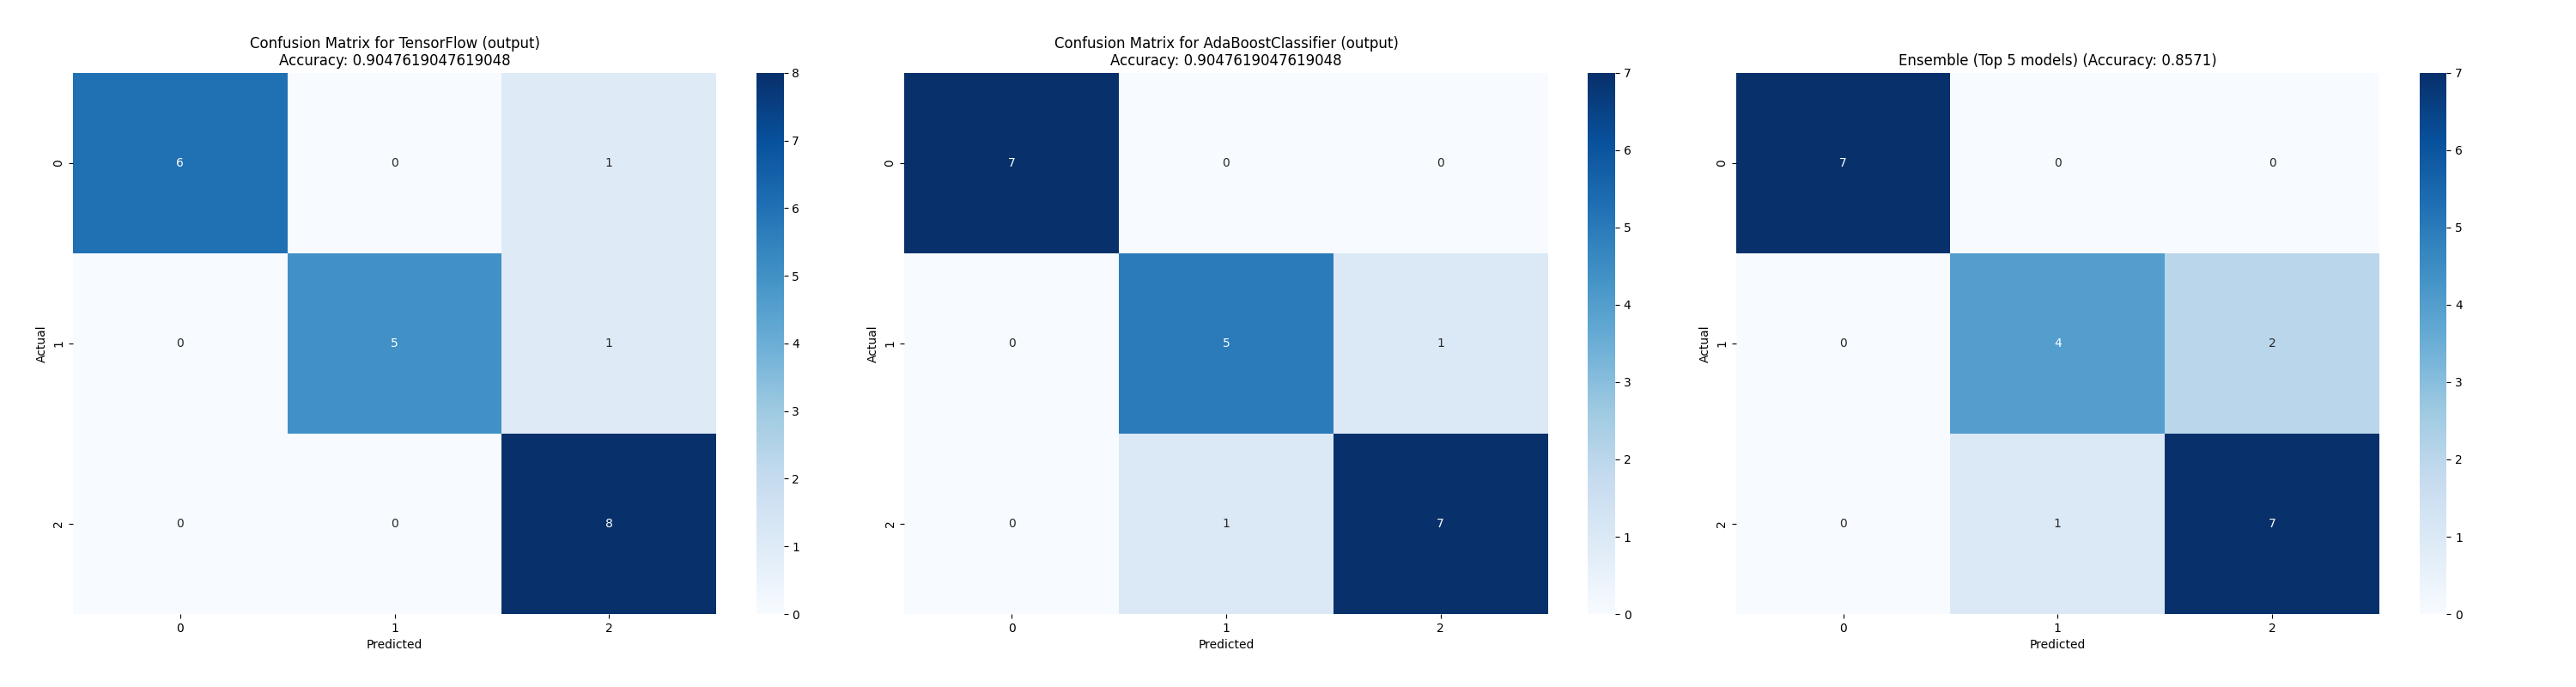
\includegraphics[width=0.95\linewidth]{class_all_section/top_2_and_ensemble_confusion_matrices_SFST_Benefit.png}
    \caption{Effect of EL on SFST Benefit using Classification and All Features}
    \label{fig_class_all:EL_SFST}
\end{figure}

This figure demonstrates why ensemble learning can reduce performance. 
In this figure, the leftmost image represents the best model, the middle image shows the second-best and the rightmost image illustrates the ensemble learning approach using the top five models. 
Since the top models have few errors that differ from model to model, when combined, these errors become more impactful. 
This example highlights the downside of ensemble learning when using small datasets. 
Overall, these results demonstrate that \ac{ML} can be used to classify wetlands using the \ac{WESP-AC} features. 
Our next section explores feature reduction techniques to reduce the input vector.

\subsubsection{Feature Reduction}\label{sec:class_all_featred}
Feature reduction involves techniques to decrease the size of the input vector while maintaining or improving model performance.
In this section, we explore the three feature reduction techniques outlined in Section \ref{sec:PA}.
Using accuracy as the primary metric, we compared the performance of algorithms for each \ac{EF} trained with reduced feature sets.
The best-performing algorithm for each function was selected based on the accuracy metrics from Table \ref{tab_class_all:model_accuracies_best}.
Each algorithm was then trained with the three reduction techniques, using a varying number of features, ranging from just two to the entire feature set.
We analyzed and compared our results through both graphical and numerical representations.
We used a training:validation split of 80:20, rather than 90:10, when training our reduced models.


Figures \ref{fig_class_all:pr_featred_graph} to \ref{fig_class_all:sfst_ben_featred_graph} in the annex illustrate the results for each \ac{EF} with the three reduction techniques.
In these figures, each \ac{EF} is presented with its corresponding accuracy across different feature counts, offering deeper insights into the impact of feature reduction on model performance.
Figures \ref{class_all_tab:featred_nr_big} and \ref{class_all_tab:featred_sfst_big} provide a closer look at the impact of feature reduction techniques on \ac{SR} Benefit and \ac{NR} Benefit, respectively.
In Figure \ref{class_all_tab:featred_nr_big}, the relationship between feature count and accuracy is highlighted, showing that as the number of features increases, accuracy improves up to a point.
It also illustrates the differences between the \ac{SKB} and \ac{VT} reduction techniques.
\ac{SKB}, using the F-classifier, achieved maximum accuracy with around 45 features, while \ac{VT} required approximately 70 features to reach a similar level.
\ac{VT} consistently performed the worst and only converged after using over 100 features with some \ac{EF}s.
This effect can be observed in figure \ref{class_all_tab:featred_sfst_big}.

\begin{figure}[h]
    \centering
    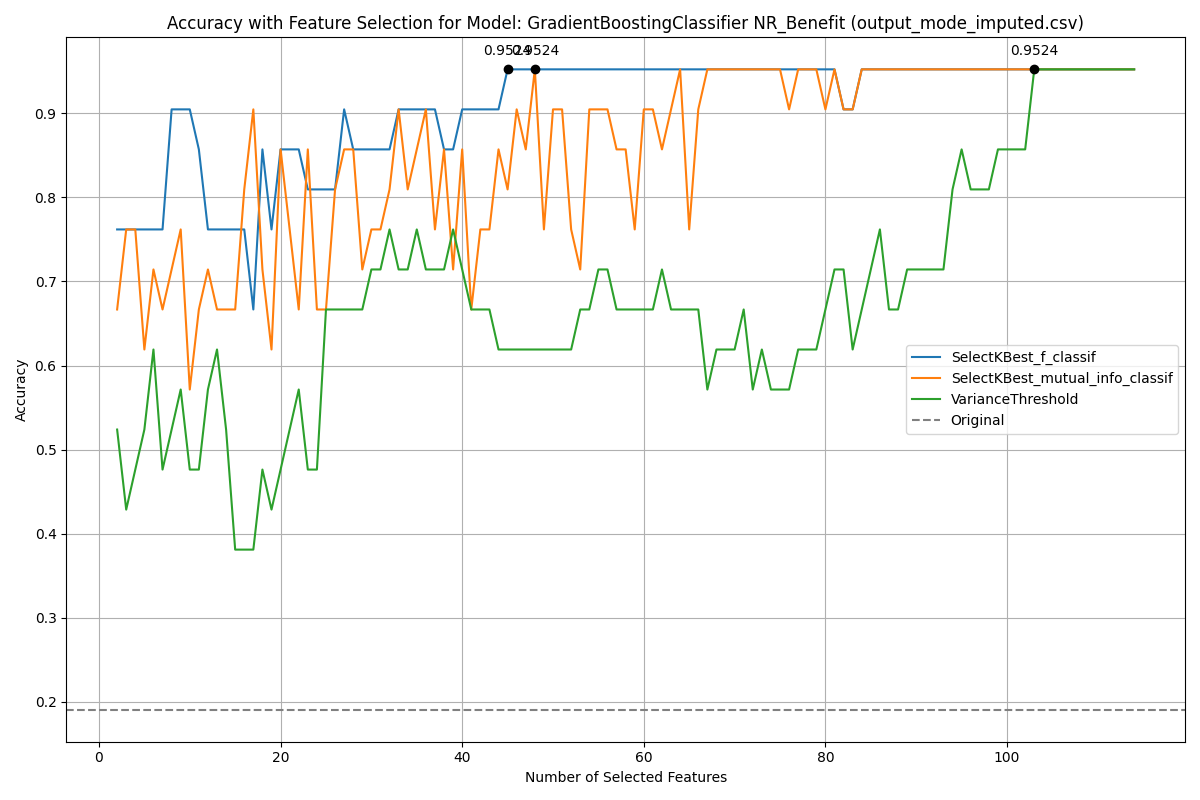
\includegraphics[width=0.85\linewidth]{class_all_section/feature_selection_accuracy_plot_output_mode_imputedcsv_GradientBoostingClassifier_NR_Benefit.png}
    \caption{NR Benefit Feature Reduction D4}
    \label{class_all_tab:featred_nr_big}
\end{figure}

\begin{figure}[h]
    \centering
    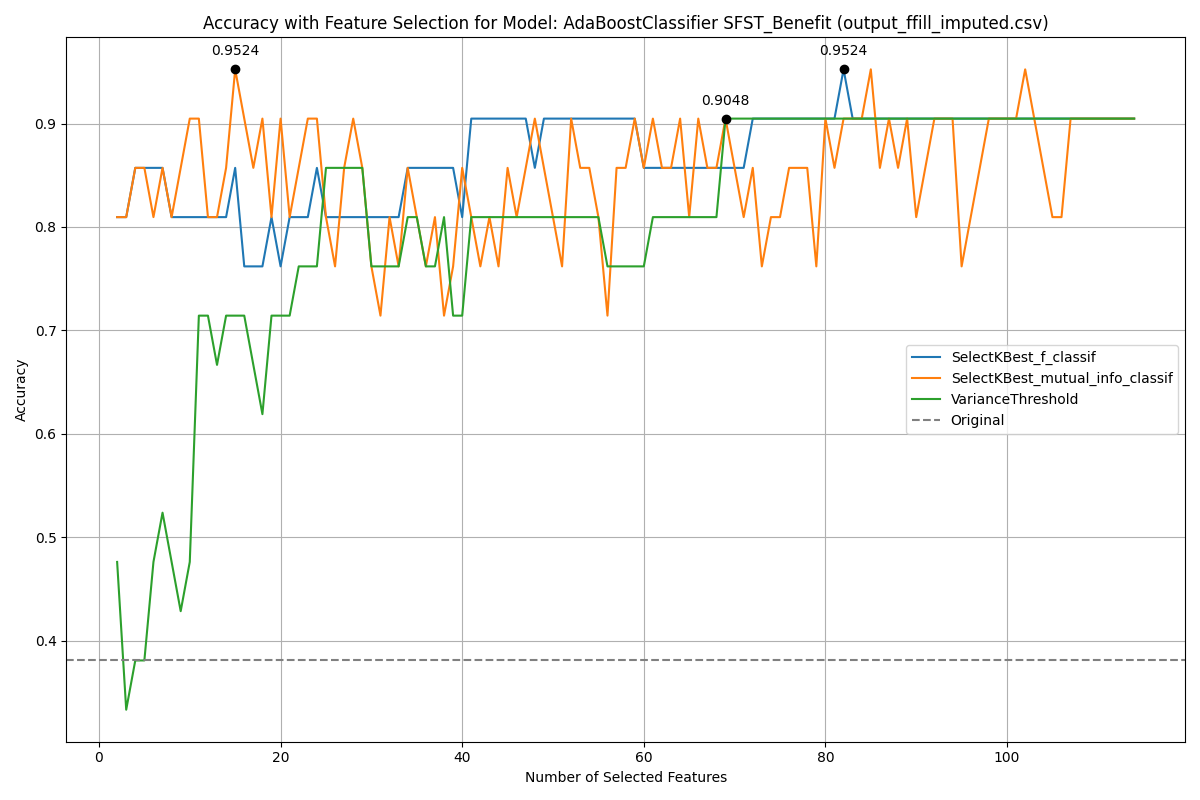
\includegraphics[width=0.85\linewidth]{class_all_section/feature_selection_accuracy_plot_output_ffill_imputedcsv_AdaBoostClassifier_SFST_Benefit.png}
    \caption{SFST Benefit Feature Reduction D4}
    \label{class_all_tab:featred_sfst_big}
\end{figure}

These results clearly demonstrate that \ac{SKB} significantly outperforms \ac{VT} in terms of both accuracy and efficiency.
Furthermore, the \ac{SKB} method enables a considerable reduction in the number of input features without compromising accuracy.
Nonethless, our feature reduction techniques have achieved interesting results.
Our findings are further validated in Table \ref{tab_class_all:featred_small}, which presents the two best overall models with significantly reduced feature sets.

\begin{longtable}{|p{3cm}|p{3cm}|p{2cm}|p{2cm}|p{2cm}|}
\hline
\textbf{Function} & \textbf{Accuracy} &  \textbf{ Features} & \textbf{2nd Accuracy} &  \textbf{2nd Features}\\ \hline
\endfirsthead
\hline
\textbf{Function} & \textbf{Accuracy} &  \textbf{ Features} & \textbf{2nd Accuracy} &  \textbf{2nd Features}\\ \hline
\endhead

PR & 85.71\% & F43, F45 & 90.45\% &  F21, F23, F24, F28, F29, F31, F43, F44, F45 \\ \hline
NR & 80.85\% & F43, F44, F45 & 76.19\% &  F43, F44 \\ \hline
SR & 71.42\% & OF22, F35, F43, F45, F49 & 61.90\% & F43, F44 \\ \hline
WS & 85.71\% & F43, F44 & 85.71\% & F31, F43 \\ \hline
SFST & 95.24\% & F1, F43 & 95.24\% & F1, F24, F43 \\ \hline
PR Benefit & 85.71\% & OF22, F41 & 90.47\% & OF22, F41, F48, F50 \\ \hline
NR Benefit & 90.48\% & OF9, OF10, OF19, OF21, F41 & 80.95 \% & OF10, OF20, F41 \\ \hline
SR Benefit & 95.24\% & OF19, F41 & 100.0\% & OF19, OF21, F41\\ \hline
WS Benefit & 80.95\% & OF17, OF23 & 95.24\% & OF17, OF24, F51\\ \hline
SFST Benefit & 57.14\% & OF22, OF28 & 57.14\% & OF18, OF22, OF28 \\ \hline
\caption{Maximum Proportionate Accuracy}
\label{tab_class_spec:featred_small}
\end{longtable}


In this table, when using a limited set of features, all \acp{EF} achieved an accuracy above 80\%, with most achieving over 90\%.
Most impressively, \ac{WS} achieved 90.45\% while \ac{SFST} achieved 95.24\% using only two features.
\ac{SR}, \ac{NR} and \ac{PR} achieved respective accuracies of 80.95\%, 80.95\% and 85.71\%.
These slightly lower accuracies compared to \ac{WS} and \ac{SFST} suggest that these \ac{EF}s may different training procedures to fully capture their complexity.
Nevertheless, the results remain impressive given the reduction in input features.
For instance, using only F43 and F44, we achieved accuracies of 80.95\% and 85.71\% for \ac{NR} and \ac{PR}, respectively.
\ac{SR} required slightly more features, utilizing F30, F31, F43, F44 and F45 to achieve 80.95\%.
\ac{WS} and \ac{SFST} performed exceptionally well, achieving accuracies of 90.45\% and 95.24\% with only two features.
\ac{WS} used F43 and F46, while \ac{SFST} relied on F43 and F44.
A clear pattern emerges, showing that features F43 to F44 are crucial in the classification of wetlands.
F43, in particular, appears to be the most influential, as it is included in all \acp{EF}.

For the Benefit ratings, the achieved accuracies were generally higher than the function ratings.
The accuracy ranged from 90.45\% to 100.00\% for the Benefit ratings, though they typically required slightly more features than the function scores.
It's noteworthy that the function ratings (e.g., \ac{NR}, \ac{PR}) did not achieve higher scores with an increased number of features.
The reduced feature accuracy was rarely higher than by using all features.
In the rare cases where accuracy was higher, it required a significant amount of features.
Regarding the classification of benefits, \ac{SR} Benefit achieved the best performance, with 100\% accuracy using four features (OF19, OF21, F21, F43) and 95.24\% using only OF19 and F41.
\ac{WS} Benefit also performed well, achieving 95.24\% accuracy with only OF17 and OF23.
The results for \ac{WS} Benefit are particularly interesting since our model relied solely on \ac{OF} features.
This approach could allow researchers to assess the \ac{WS} Benefit of wetlands without needing to visit the site.

\ac{NR} Benefit struggled to achieve high accuracy with fewer features.
For example, it reached only 76.19\% accuracy with three features (OF10, F43, F44) but achieved 90.45\% with eight features.
This indicates that some functions may require significantly more features due to their inherent complexity.
Similarly, \ac{PR} Benefit achieved 90.45\% with six features and 85.71\% using only F41 and F43.
Finally, \ac{SFST} Benefit achieved 90.45\% with ten features and 80.95\% using F43 and F44.
These results highlight the differences between function and Benefit ratings.
Both types of ratings performed well with a limited number of features, but the Benefit ratings required slightly more features to achieve higher accuracies.
This could be explained by the fact that the benefit of a wetland may be highly complex in nature.
Overall, features F41 to F43 seem to be critical for both function and Benefit ratings.
Additionally, the benefit ratings seem to be more influenced by \ac{OF} features than the function ratings.
This can be explained by the fact that an \ac{EF} function is mostly related to on-site activities such as vegetation, soil and water.
On the contrary, the benefit is more influenced by human activities, which can be gathered without visiting the site.
Both Provincial and Federal classes appear to play a role in predicting certain \acp{EF}, likely because these features represent multiple features.
Overall, the extra features did not seem to benefit our models with the exception of a few \ac{EF}.

\paragraph{Ensemble Learning}
To further improve the performance of our feature reduction approach, we implemented ensemble learning.
This technique is designed to average out errors and enhance performance without the need for retraining or complex algorithms.
Our ensemble model for each \ac{EF} was based on the top five models from the feature reduction process, using no more than ten features per model.

Table \ref{tab_class_all:featred_ensemble} shows the performance of each function before and after applying ensemble learning.

\begin{longtable}{|p{2cm}|p{2cm}|p{2cm}|p{2cm}|p{4cm}|}
\hline
\textbf{Function} & \textbf{Best Acc.} & \textbf{2nd Best Acc.} & \textbf{Ensemble Learning Acc.} & \textbf{Features Used} \\ \hline
PR & 90.48\% & 85.71\% & 85.71\% & F1, F14, F28, F29, F43, F44, F45, FedClass, ProvClass \\ \hline
NR & 80.95\% & 80.95\% & 76.19\% & F43, F44, F45, F46 \\ \hline
SR & 80.95\% & 80.95\% & 80.95\% & F1, F14, F24, F28, F29, F30, F31, F3e, F41, F43, F44, F45, F46, FedClass, OF22, ProvClass \\ \hline
WS & 90.48\% & 90.48\% & 90.48\% & F43, F44, F45, F46 \\ \hline
SFST & 95.24\% & 95.24\% & 95.24\% & F43, F44, F45, F46 \\ \hline
PR Benefit & 90.48\% & 85.71\% & 85.71\% & F14, F24, F41, F43, F44, F46, F47 \\ \hline
NR Benefit & 90.48\% & 90.48\% & 85.71\% & F1, F14, F31, F3d, F41, F43, F44, F46, MossCover, OF10, OF19, OF9 \\ \hline
SR Benefit & 100.00\% & 100.00\% & 95.24\% & F14, F28, F29, F41, F43, F44, OF19, OF21 \\ \hline
WS Benefit & 95.24\% & 95.24\% & 95.24\% & F50, F52, F54, OF17, OF23, OF7 \\ \hline
SFST Benefit & 90.48\% & 85.71\% & 85.71\% & F1, F14, F23, F31, F43, F44, F45, F46, F5, Moss Cover, ProvClass \\ \hline
\caption{Ensemble Learning Accuracy}
\label{tab_class_all:featred_ensemble}
\end{longtable}

In this table we present the accuracy of the best and second model, the ensemble learning accuracy and the features used for ensemble learning.

The top two models in this table are not necessarily the same as those in Table \ref{tab_class_all:featred_small}.
The five models chosen for ensemble learning were selected purely based on the highest accuracy with fewer than ten features, aiming to minimize bias.
This table confirms our earlier observation that ensemble learning can sometimes reduce accuracy.
Indeed, seven out of ten \acp{EF} experienced an approximate 5\% drop in accuracy, while the others remained unchanged.
Additionally, the number of features used was significantly increased with ensemble learning.
However, ensemble learning could still be beneficial if more training data was available.
Ensemble learning typically requires larger datasets than those we used.
Given the smaller size of our dataset, our validation data was limited to approximately 40 sites, meaning a single error could reduce the overall accuracy by 2.5\%.
This also indicates that the ensemble learning approach can be significantly impacted by a single misclassification.
As a result, ensemble learning did not enhance our algorithms as expected.
Nonetheless, even without ensemble learning, our feature reduction techniques yielded strong performance.


\subsection{Specific Features}\label{sec:class_spec}
This section utilizes our D2 datasets, which consist solely of features specific to each \ac{EF}.
This significantly reduces the input vector from over 100 features to a range of six to 33.
As in the previous section, we compared our results across various data filling methods; however, only the best results are presented.

First, we present the training results and the ensemble learning approach using all D2 features in Section \ref{sec:class_specific_results}.
Our ensemble learning algorithm combines the top five best-performing algorithms, with predictions averaged to improve overall accuracy.

Section \ref{sec:class_specific_featred} details our feature reduction approach, leveraging the results from Section \ref{sec:class_specific_results}.
In this section, we evaluate the performance of our approach for each \ac{EF} based on prediction accuracy.
Our goal, as in the previous section, is to achieve strong performance with the fewest possible features.
We also investigate the impact of applying ensemble learning to the reduced feature models, aiming to enhance accuracy while maintaining a streamlined feature set.



\subsubsection{Training Results}\label{sec:class_specific_results}
First, we performed a grid search of our algorithms, hyperparameters and data filling methods on our D2 dataset.
Table \ref{tab_class_specific:model_accuracies_best} provides an overview of the best-performing algorithms for each \ac{EF}.

\begin{table}[H]
\centering
\begin{tabular}{|c|c|p{4cm}|c|}
\hline
\textbf{Function} & \textbf{Model} & \textbf{Data} & \textbf{Accuracy} \\
\hline
PR & Ridge & All Data & 95.24\% \\
\hline
NR    & SGD & Mean & 90.48\% \\
\hline
SR    & TensorFlow & Median & 100.00\% \\
\hline
WS    & GradientBoosting & All Data & 100.00\% \\
\hline
SFST  & GradientBoosting & All data & 95.24\% \\
\hline
PR Ben. & KNeighbors & All Data & 95.24\% \\
\hline
NR Ben. & SVC & All Data & 100.00\% \\
\hline
SR Ben.& Ridge, GradientBoosting & All Data & 100.0\% \\
\hline
WS Ben. & RandomForest & BFill, Custom, Interpolated, Iterative, Mean, Median, Mode & 95.24\% \\
\hline
SFST Ben. &  RandomForest & Custom, Mean & 71.42\% \\
\hline
\end{tabular}
\caption{Best Model Accuracies}
\label{tab_class_specific:model_accuracies_best}
\end{table}

In this table, each \ac{EF} is shown with the accuracy of the best-performing model and data filling method.
A slight increase in performance can be observed when comparing these results with the results from using D4, found in Table \ref{tab_class_all:model_accuracies_best}.
In fact, the accuracy has increased for five \acp{EF}, remained unchanged for four and was reduced for one \ac{EF}.
Most impressively, using only specific features, we achieved an accuracy of 100\% on five \acp{EF}.
Notably, \ac{SR} increased from 90.48\% to 100.00\% and \ac{NR} from 80.95\% to 90.48\%.
However, \ac{SFST} Benefit was considerably reduced from 95.24\% in the previous section to 71.42\%.
We thoroughly verified these results and determined that a feature present in D4 but not in D2 is crucial for this \ac{EF}.
Comparing the specific features for \ac{SFST} Benefit and the results from feature reduction using all features in Table \ref{tab_class_all:featred_small} highlights this gap.
\ac{SFST} Benefit appears to be mostly dependent on \ac{OF} questions, while using all features demonstrated that \ac{F} features are among the most important.
Questions remain as to why our models using specific features did not perform well for \ac{SFST} Benefit.
The data may be highly uncorrelated when using specific features, which could hinder the model's ability to learn.
Nonetheless, we achieved very good performance on all other \acp{EF} using only specific features.

To further improve the performance of our algorithms, we proposed using ensemble learning to combine multiple models.
Overall, ensemble learning did not consistently enhance the performance of our algorithms, as shown in Table \ref{tab_class_specific:class_ensemble}.

\begin{table}[H]
\centering
\begin{tabular}{|c|c|c|}
\hline
\textbf{Function} & \textbf{Accuracy} & \textbf{Ensemble Accuracy} \\
\hline
PR      & 95.24\% & 95.24\% \\
\hline
NR      & 90.46\% & 85.71\%\\
\hline
SR      & 100.00\% & 100.00\%\\
\hline
WS      & 100.00\% & 100.00\%\\
\hline
SFST    & 95.24\% & 95.24\%\\
\hline
PR Ben. & 95.24\% & 100.00\%\\
\hline
NR Ben. & 100.00\% & 100.00\%\\
\hline
SR Ben. & 100.0\% & 100.0\%\\
\hline
WS Ben. & 95.24\% & 95.24\%\\
\hline
SFST Ben. & 71.42\% & 76.19\%\\
\hline
\end{tabular}
\caption{Ensemble Model Accuracies}
\label{tab_class_specific:class_ensemble}
\end{table}

\ac{SFST} Benefit was slightly improved through ensemble learning, increasing from 71.42\% to 76.19\%.
Similarly, \ac{PR} Benefit increased from 95.24\% to 100.00\%.
Figures \ref{fig_class_specific:EL_PR} and \ref{fig_class_specific:EL_SFST_ben} show \ac{PR} Benefit and \ac{SFST} Benefit using the top two models and ensemble learning, respectively.

\begin{figure}
    \centering
    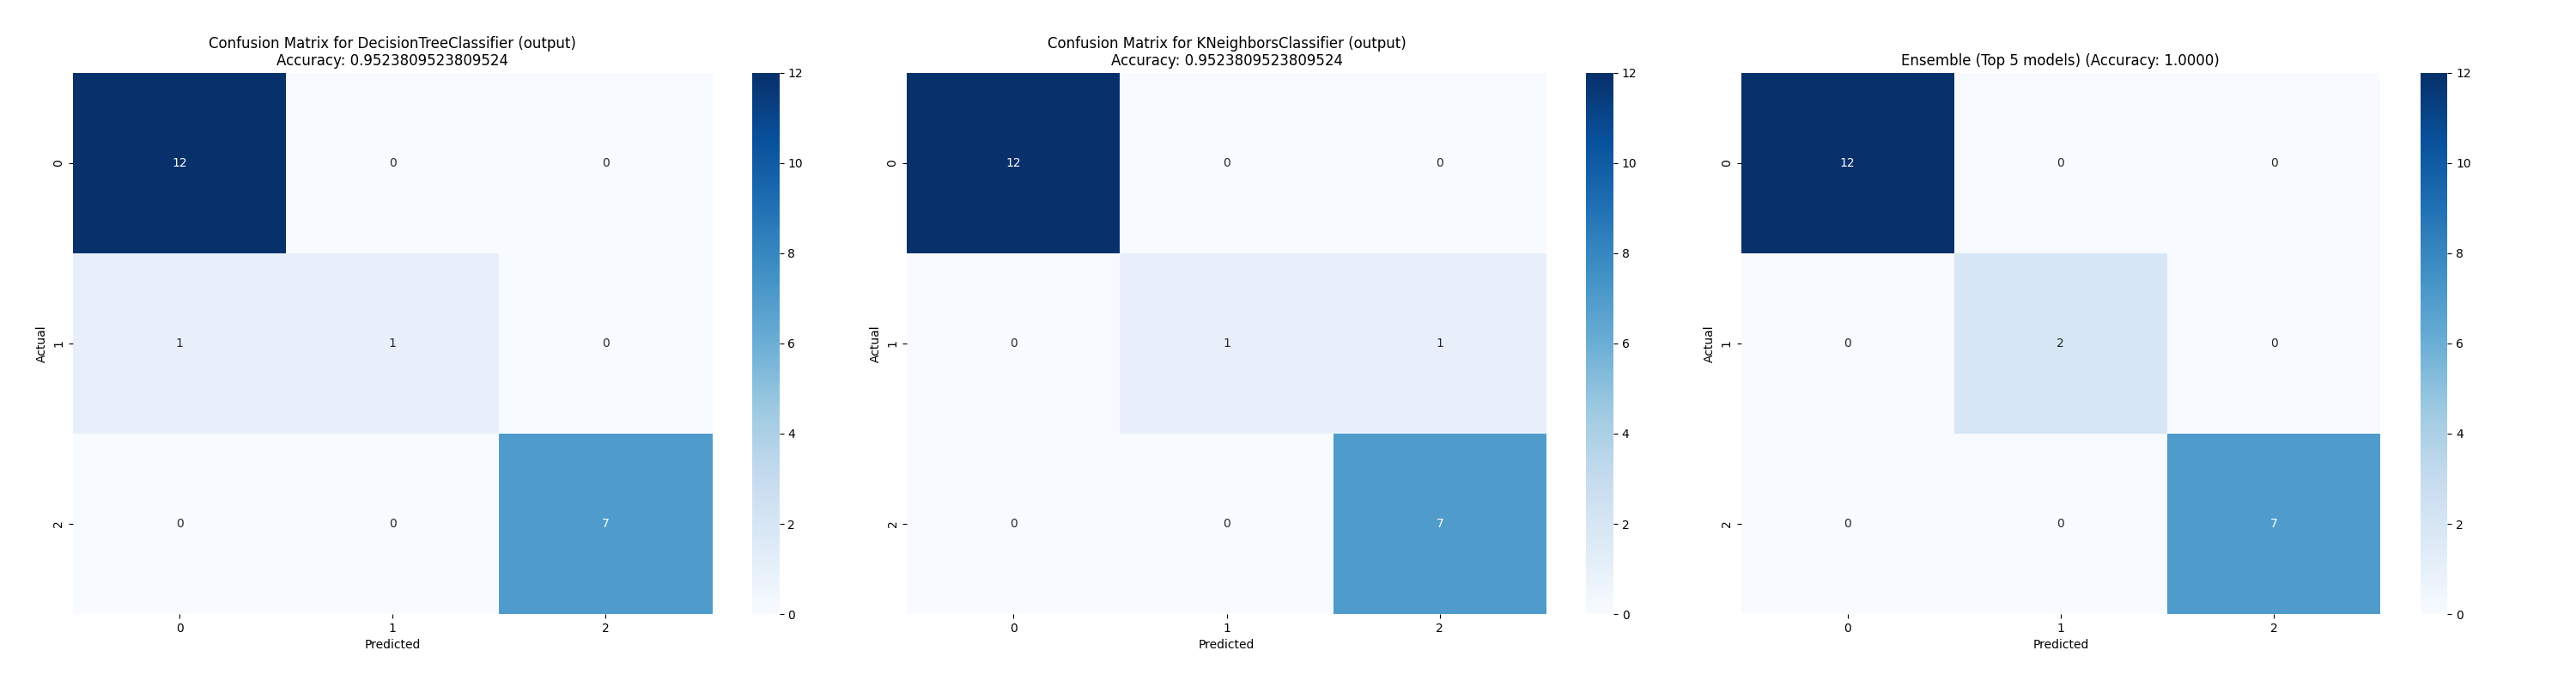
\includegraphics[width=0.95\linewidth]{class_specific_section/top_2_and_ensemble_confusion_matrices_PR_Benefit.png}
    \caption{Effect of EL on PR Benefit using Classification and Specific Features}
    \label{fig_class_specific:EL_PR}
\end{figure}

\begin{figure}
    \centering
    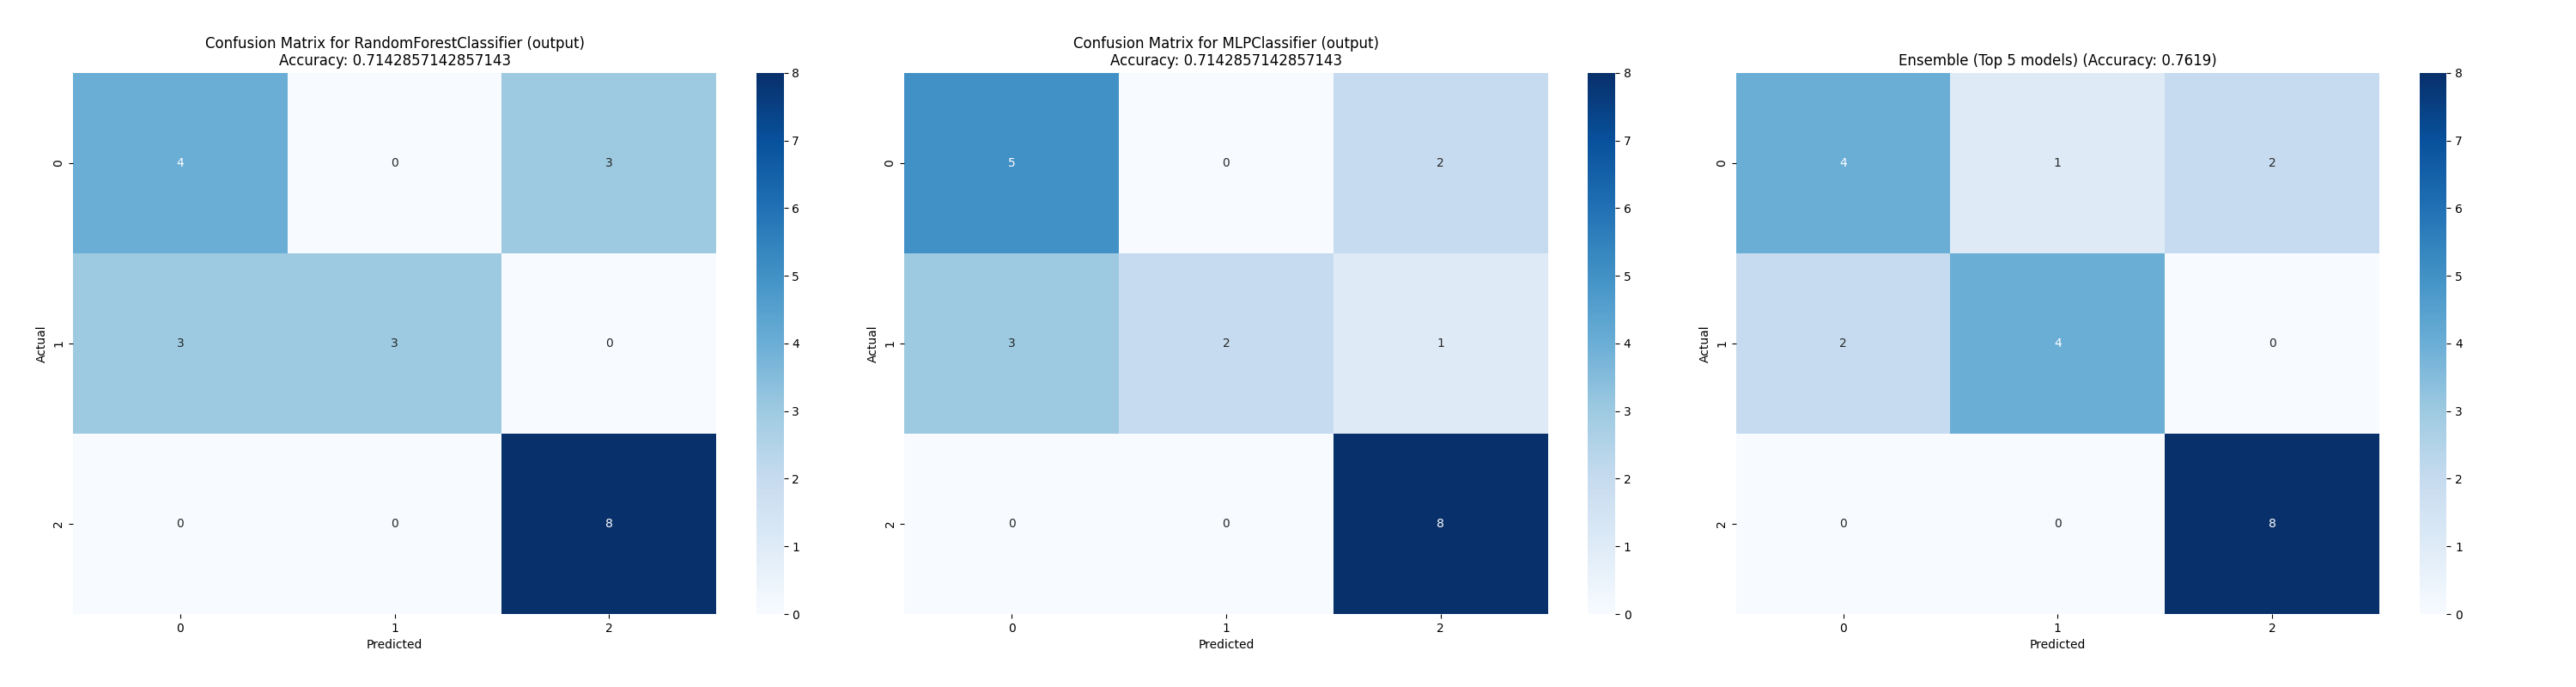
\includegraphics[width=0.95\linewidth]{class_specific_section/top_2_and_ensemble_confusion_matrices_SFST_Benefit.png}
    \caption{Effect of EL on SFST Benefit using Classification and Specific Features}
    \label{fig_class_specific:EL_SFST_ben}
\end{figure}

In these figures, we see how ensemble learning can enhance results by averaging bad predictions into their correct classes.

\subsubsection{Feature Reduction}\label{sec:class_specific_featred}
As with D4, we applied feature reduction techniques to minimize the input feature vector of our D2 dataset.
In this section, we explore the three feature reduction techniques outlined earlier in Section \ref{sec:PA}.
Using accuracy as the primary metric, we compared the algorithms for each \ac{EF} trained with reduced features.
The best-performing algorithm for each function was selected based on the training accuracy from Table \ref{tab_class_specific:model_accuracies_best}.
Each algorithm was trained with the three reduction techniques, utilizing features ranging from two to all features specific to the \ac{EF}.

Table \ref{tab_class_spec:featred_small} presents the two best overall models for each \ac{EF} with reduced features.

\begin{longtable}{|p{3cm}|p{3cm}|p{2cm}|p{2cm}|p{2cm}|}
\hline
\textbf{Function} & \textbf{Accuracy} &  \textbf{ Features} & \textbf{2nd Accuracy} &  \textbf{2nd Features}\\ \hline
\endfirsthead
\hline
\textbf{Function} & \textbf{Accuracy} &  \textbf{ Features} & \textbf{2nd Accuracy} &  \textbf{2nd Features}\\ \hline
\endhead

PR & 85.71\% & F43, F45 & 90.45\% &  F21, F23, F24, F28, F29, F31, F43, F44, F45 \\ \hline
NR & 80.85\% & F43, F44, F45 & 76.19\% &  F43, F44 \\ \hline
SR & 71.42\% & OF22, F35, F43, F45, F49 & 61.90\% & F43, F44 \\ \hline
WS & 85.71\% & F43, F44 & 85.71\% & F31, F43 \\ \hline
SFST & 95.24\% & F1, F43 & 95.24\% & F1, F24, F43 \\ \hline
PR Benefit & 85.71\% & OF22, F41 & 90.47\% & OF22, F41, F48, F50 \\ \hline
NR Benefit & 90.48\% & OF9, OF10, OF19, OF21, F41 & 80.95 \% & OF10, OF20, F41 \\ \hline
SR Benefit & 95.24\% & OF19, F41 & 100.0\% & OF19, OF21, F41\\ \hline
WS Benefit & 80.95\% & OF17, OF23 & 95.24\% & OF17, OF24, F51\\ \hline
SFST Benefit & 57.14\% & OF22, OF28 & 57.14\% & OF18, OF22, OF28 \\ \hline
\caption{Maximum Proportionate Accuracy}
\label{tab_class_spec:featred_small}
\end{longtable}


At first glance, this dataset underperformed compared to D4, with accuracies ranging from 71.42\% to 95.24\%.
When using D2, all \acp{EF} achieved lower accuracies than those achieved using the reduced feature set from the D4 dataset.
\ac{SFST} Benefit was the most significantly impacted, with its accuracy dropping from 80.95\% using two features to 57.14\%.
Overall, it seems that using all available features and then applying feature reduction techniques yields better results than using only specific features from the outset.
This discrepancy could be due to certain features, absent in D2, that capture complex interactions or provide unique insights not available in the specific feature set.
Figures \ref{fig_class_spec:pr_featred_graph} to \ref{fig_class_spec:sfst_ben_featred_graph} in the annex demonstrate the effect of the various feature reduction techniques.
Figure \ref{class_spec_tab:featred_pr} highlights the impact of feature reduction on \ac{WS}.

\begin{figure}[h]
    \centering
    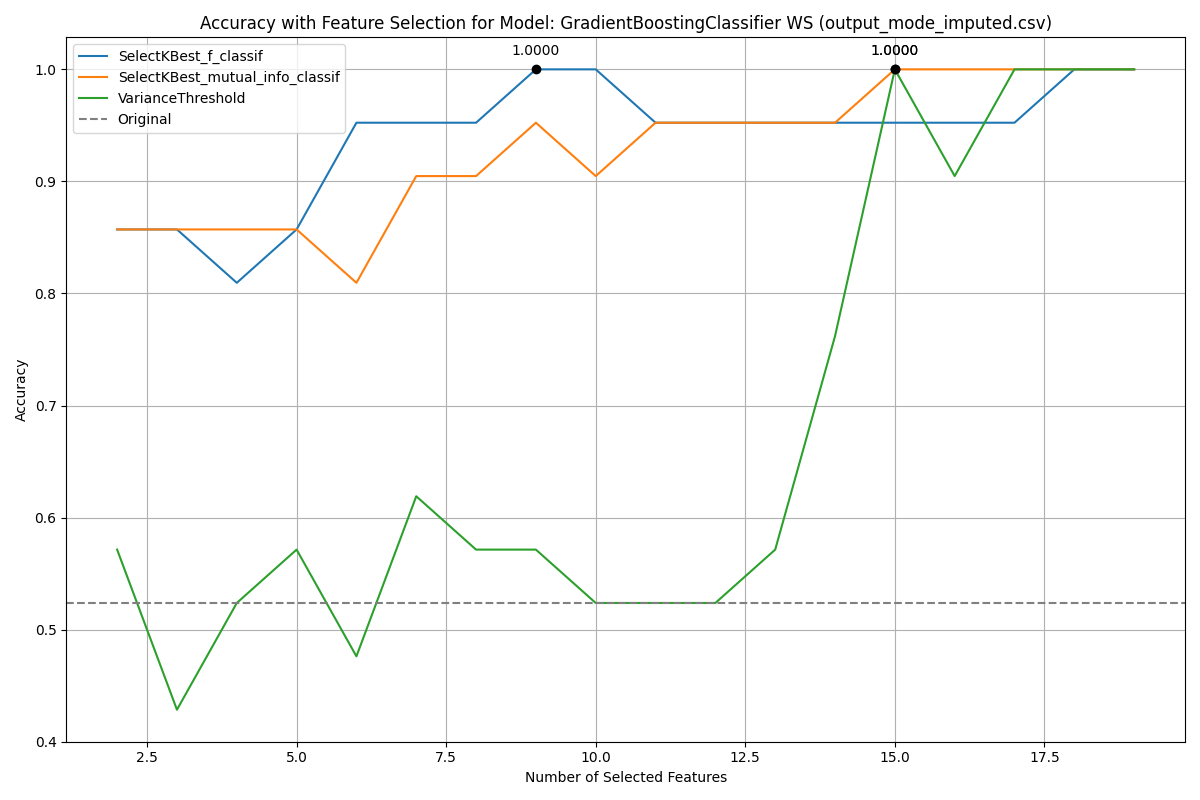
\includegraphics[width=0.85\linewidth]{class_specific_section/images_class_ensemble_reduction/feature_selection_accuracy_plot_output_mode_imputedcsv_GradientBoostingClassifier_WS.png}
    \caption{WS Feature Reduction D4}
    \label{class_spec_tab:featred_pr}
\end{figure}

In this figure, the earlier-mentioned difference between \ac{SKB} and \ac{VT} is clearly visible once again.
\ac{SKB} significantly outperformed \ac{VT}, converging more quickly and efficiently.
In fact, \ac{SKB} with F-classifier achieved 100.00\% accuracy using nine features, while \ac{VT} required 15.
This figure underscores the importance of carefully analyzing results to better understand the behavior of different reduction techniques.

\paragraph{Ensemble Learning}
To further enhance the performance of our feature reduction approach, we proposed using ensemble learning.
This technique is designed to average out errors and improve performance without retraining or the need for complex algorithms.
Our ensemble model for each \ac{EF} is based on the top five models derived from feature reduction, with no more than 10 features per model.

Table \ref{tab_class_spec:featred_ensemble} shows the performance for each function before and after applying ensemble learning.

\begin{longtable}{|p{2cm}|p{2cm}|p{2cm}|p{2cm}|p{4cm}|}
\hline
\textbf{Function} & \textbf{Best Acc.} & \textbf{2nd Best Acc.} & \textbf{Ensemble Learning Acc.} & \textbf{Features Used} \\ \hline
PR & 90.48\% & 85.71\% & 85.71\% & F1, F14, F28, F29, F43, F44, F45, FedClass, ProvClass \\ \hline
NR & 80.95\% & 80.95\% & 76.19\% & F43, F44, F45, F46 \\ \hline
SR & 80.95\% & 80.95\% & 80.95\% & F1, F14, F24, F28, F29, F30, F31, F3e, F41, F43, F44, F45, F46, FedClass, OF22, ProvClass \\ \hline
WS & 90.48\% & 90.48\% & 90.48\% & F43, F44, F45, F46 \\ \hline
SFST & 95.24\% & 95.24\% & 95.24\% & F43, F44, F45, F46 \\ \hline
PR Benefit & 90.48\% & 85.71\% & 85.71\% & F14, F24, F41, F43, F44, F46, F47 \\ \hline
NR Benefit & 90.48\% & 90.48\% & 85.71\% & F1, F14, F31, F3d, F41, F43, F44, F46, MossCover, OF10, OF19, OF9 \\ \hline
SR Benefit & 100.00\% & 100.00\% & 95.24\% & F14, F28, F29, F41, F43, F44, OF19, OF21 \\ \hline
WS Benefit & 95.24\% & 95.24\% & 95.24\% & F50, F52, F54, OF17, OF23, OF7 \\ \hline
SFST Benefit & 90.48\% & 85.71\% & 85.71\% & F1, F14, F23, F31, F43, F44, F45, F46, F5, Moss Cover, ProvClass \\ \hline
\caption{Ensemble Learning Accuracy}
\label{tab_class_all:featred_ensemble}
\end{longtable}


In this table, the first column lists the \ac{EF}, while the second and third columns display the best and second-best accuracy from Section \ref{sec:class_specific_featred} using a maximum of 10 features.
The fourth column represents the accuracy of the ensemble learning model and the last column lists the features of all five models used for ensemble learning.
As seen in previous sections, ensemble learning did not lead to an increase in the performance of our models.

\subsection{Dataset Comparison}
To facilitate a clear comparison of the results, we present the best-performing models for each \ac{EF} using both all features and specific features.
The models that yielded the most notable outcomes are summarized in Table \ref{tab_combined:featred_accuracy}.

\begin{longtable}{|p{3cm}|p{2cm}|p{3cm}|p{2cm}|p{3cm}|}
\hline
\textbf{Function} & \textbf{Acc. All} & \textbf{Features All} & \textbf{Acc. Specific} & \textbf{Features Specific} \\ \hline
\endfirsthead
\hline
\textbf{Function} & \textbf{Acc. All} & \textbf{Features All} & \textbf{Acc. Specific} & \textbf{Features Specific} \\ \hline
\endhead

PR & 85.71\% & F43, F45 & 85.71\% & F43, F45 \\ \hline
NR & 80.95\% & F43, F44 & 80.85\% & F43, F44, F45 \\ \hline
SR & 80.95\% & Hydrogeo., F24, F29, F43, F44, F45 & 71.42\% & OF22, F35, F43, F45, F49 \\ \hline
WS & 90.45\% & F43, F46 & 85.71\% & F43, F44 \\ \hline
SFST & 95.24\% & F43, F44 & 95.24\% & F1, F43 \\ \hline
PR Benefit & 90.45\% & F14, F24, F41, F43, F46, F47 & 85.71\% & OF22, F41 \\ \hline
NR Benefit & 90.45\% & MossCover, OF9, OF10, OF19, F1, F14, F41, F43 & 90.48\% & OF9, OF10, OF19, OF21, F41 \\ \hline
SR Benefit & 100.00\% & OF19, OF21, F41, F43 & 95.24\% & OF19, F41 \\ \hline
WS Benefit & 95.24\% & OF17, OF23 & 80.95\% & OF17, OF23 \\ \hline
SFST Benefit & 90.45\% & ProvClass, MossCover, F1, F5, F23, F31, F43, F44, F45, F46 & 57.14\% & OF22, OF28 \\ \hline
\caption{Comparison of Best Accuracy and Features from Two Tables}
\label{tab_combined:featred_accuracy}
\end{longtable}

Table \ref{tab_combined:featred_accuracy} illustrates that classification using all features generally outperforms using specific features.
The accuracy for several \acp{EF}, such as \ac{SR} and \ac{SFST} Benefit, decreased significantly when specific features were employed.
This reduction in accuracy suggests that some critical features may be absent in the D2 dataset.
For example, \ac{SFST} Benefit's accuracy dropped from 90.45\% to 57.14\%, indicating the importance of certain features available only in the D4 dataset.

Conversely, some \acp{EF}, such as \ac{PR} and \ac{WS}, maintained consistent accuracy across both datasets, highlighting the robustness of the selected features in these cases.
The results for \ac{WS} Benefit are particularly noteworthy, as the model achieved a high accuracy of 95.24\% using only \ac{OF} features.
This finding is significant because it suggests that \ac{WS} Benefit can potentially be analyzed without requiring field data, which could significantly simplify the analysis process.

However, other \acp{EF}, such as \ac{NR} Benefit, required a larger number of features to achieve satisfactory accuracy.
This complexity could be due to the intricate nature of these \acp{EF}, which necessitate more comprehensive data for accurate classification.
Overall, while feature reduction techniques can simplify the model and reduce the required data, they may also result in a loss of accuracy, particularly for more complex \acp{EF}.

The application of ensemble learning produced mixed results. While some \acp{EF} benefited from the approach, others experienced reduced accuracy.
Future research should focus on identifying the optimal balance between feature reduction and model accuracy, potentially by exploring additional feature selection techniques or expanding the dataset to include more diverse wetland types.
Moreover, the exploration of more advanced ensemble learning methods or hybrid models could further improve classification accuracy, especially for the more complex \acp{EF}.




\section{Regression}\label{sec:regression}
Regression is a common type of algorithm used in \ac{ML} with a key difference from classification.
Classification predicts a class, such as lower, moderate our higher, while regression predicts a continuous value.
In our case, the continuous value would be the score for the function or benefit of an \ac{EF}.
The classification results from \ref{sec:class} have shown great promise and is interesting for the project.
However, the algorithms trained for classification used the normalized scores, for both the function and benefit.
In turn, the algorithms are specific to regions, such as for NB and depend on the calibration wetlands.
If different calibration wetlands are used or the region modified, the algorithms could underperform significantly.
For this reason, we propose using regression to predict the non-normalized and normalized scores of the various \ac{EF}.
We propose using the non-normalize score such that it does our approach does not depend on calibration sites or region.
However, we also compare using pre-normalized scores to compare the results.
The data was collected, modified and generated using simple pre-processing techniques as seen from section \ref{sec:data}.
We present our results using both D4 and D2 datasets, respectively using all features and specific features.
We use the Mean Squared Error (MSE) as metric, which averages the squares of the errors and is defined in equation \ref{eq:mse}.
\begin{equation}
\text{MSE} = \frac{1}{n} \sum_{i=1}^n (y_i - \hat{y}_i)^2
\label{eq:mse}
\end{equation}

\subsection{All Features}
Similar to our classification technique, we perform a grid search of various regression algorithms, hyperparameters and data filling methods.
We trained our algorithms and techniques for \ac{PR}, \ac{NR}, \ac{SR}, \ac{WS} and \ac{SFST}, for both the Function and Benefit.
More information about the training procedure can be found within the GITHUB, under regression.
The algorithms used for regression are shown in table \ref{tab:all_algorithms}.
Similar to classification, we first propose comparing the regression algorithms using all features for the \ac{EF}.
We compare our training results, feature reduction techniques and class grouping.
Class grouping consists of classifying the regression predictions such that we can compare our regression and classification.
We perform the same tests using our D2 datasets which consists of specific features only.

\subsubsection{Training Results}
First, we show the training results using the top accuracy over any algorithm and data filling method in table \ref{reg_all_tab:mse_summary}.
This table shows the MSE for the \ac{NNorm}, \ac{Norm} and \ac{PNorm} of the best models.
Using this figure, we can see a significantly increase in MSE when comparing \ac{NNorm} and Norm.
In fact, the MSE is often doubled when normalizing the prediction from using \ac{NNorm}.
This is expected since normalizing predictions scales the errors into a bigger scale.
When comparing \ac{NNorm} and \ac{PNorm}, \ac{NNorm} achieved better results for most \ac{EF}s.
When looking at \ac{EF} Benefits, \ac{NNorm} performed better on \ac{PR} and \ac{WS} while \ac{PNorm} performed better on \ac{SR}, \ac{NR} and \ac{WS}. 
\ac{NNorm} achieved an MSE of 1.19 for \ac{WS} Benefit while \ac{PNorm} achieved a lower MSE of 0.63.
On the contrary, \ac{PNorm} achieved an MSE of 0.49 for \ac{PR} Benefit while \ac{NNorm} achieved 0.22.
This difference in results demonstrates the purpose of comparing both \ac{NNorm} and \ac{PNorm} data. 

\begin{table}[H]
\centering
\begin{tabular}{|c|c|c|c|}
\hline
\textbf{Feature} & \textbf{\ac{NNorm} MSE} & \textbf{\ac{Norm} MSE} & \textbf{\ac{PNorm} MSE} \\
\hline
NR & 0.17 & 0.48 & 0.31 \\
\hline
PR & 0.12 & 0.19 & 0.21 \\
\hline
SR & 0.37 & 0.62 & 0.46 \\
\hline
SFST & 0.20 & 0.33 & 0.26 \\
\hline
WS & 0.25 & 0.49 & 0.60 \\
\hline
NR Benefit & 0.39 & 0.45 & 0.28 \\
\hline
PR Benefit & 0.22 & 0.23 & 0.49 \\
\hline
SR Benefit & 0.17 & 0.22 & 0.07 \\
\hline
SFST Benefit & 0.51 & 0.98 & 0.71 \\
\hline
WS Benefit & 1.19 & 1.21 & 0.63 \\
\hline
\end{tabular}
\caption{Summary of Best MSE for Non-Normalized, Normalized and Pre-Normalized Data}
\label{reg_all_tab:mse_summary}
\end{table}


In the annex, tables \ref{reg_all_tab:norm_mse} and \ref{reg_all_tab:pre_norm_mse} respectively show the full results for the \ac{NNorm}, \ac{Norm} and \ac{PNorm} data.
In terms of algorithm, the AdaBoost regressor has achieved an overall better performance.
The MLP and SGD regressor were also found to be effective at predicting the scores.
In terms of data filling method, each \ac{EF} had their best performing method but overall each performed similarly.
The results presented in this section demonstrated interesting results.
It showed that both \ac{NNorm} and \ac{PNorm} data can be used for regression while \ac{Norm} should not be prioritized.


We also implemented ensemble learning in the goal to increase our performance.
Table \ref{reg_all_tab:ensemble} presents the results with and without ensemble learning for all three normalization.
In this table, we can see that our results were not significantly impacted by ensemble learning.
The MSE for \ac{NR} Benefit using \ac{NNorm} was slightly reduced from 0.39 to 0.27 while \ac{WS} Benefit was reduced to 0.86 from 1.19.
This small increase in performance could be beneficial for our class grouping.


\begin{table}[H]
\centering
\begin{tabular}{|c||c|c|c||c|c|c|}
\hline
\multirow{2}{*}{\textbf{Feature}} & \multicolumn{3}{c||}{\textbf{Training}} & \multicolumn{3}{c|}{\textbf{Ensemble Learning}} \\
\cline{2-7}
 & \textbf{Non-Norm} & \textbf{Norm} & \textbf{Pre-Norm} & \textbf{Non-Norm} & \textbf{Norm} & \textbf{Pre-Norm} \\
\hline
PR & 0.12 & 0.19 & 0.21 & 0.12 & 0.19 & 0.22 \\
\hline
NR & 0.17 & 0.48 & 0.31 & 0.17 & 0.48 & 0.28 \\
\hline
SR & 0.37 & 0.62 & 0.46 & 0.39 & 0.65 & 0.50\\
\hline
WS & 0.25 & 0.49 & 0.60 & 0.25 & 0.49 & 0.61 \\
\hline
SFST & 0.20 & 0.33 & 0.26 & 0.21 & 0.36 & 0.27\\
\hline
NR Benefit & 0.39 & 0.45 & 0.28 & 0.27 & 0.64 & 0.36 \\
\hline
PR Benefit & 0.22 & 0.23 & 0.49 & 0.31 & 0.32 & 0.31 \\
\hline
SR Benefit & 0.17 & 0.22 & 0.07 & 0.13 & 0.17 & 0.06 \\
\hline
WS Benefit & 1.19 & 1.21 & 0.63 & 0.86 & 0.87 & 0.68 \\
\hline
SFST Benefit & 0.51 & 0.98 & 0.71 & 0.38 & 0.72 & 0.60 \\
\hline
\end{tabular}
\caption{Ensemble Learning Effect on All Features Training}
\label{reg_all_tab:ensemble}
\end{table}

In the annex, figures \ref{reg_all_fig:pr_ensemble} to \ref{reg_all_fig:sfst_ben_ensemble} show graphs with the algorithms and ensemble learning.
In these figures, we present all three normalization techniques with each their top three models and their ensemble approach.
When looking at the overall clusters of normalization for each \ac{EF}, we can observe the difference between \ac{Norm} or \ac{PNorm} and \ac{NNorm} data.
Normalized data, either post or pre-normalized, were more spread out while non-normalized data was often in small clusters.
This demonstrates the benefit of using normalized data since it provides a more usable range.
However, it also showcases the issue with using pre-normalized data.
When using pre-normalized data, our model is bounded by the normalization unless the model is retrained.
Using our models to predict non-normalize scores while normalizing the predictions offers the benefits without the issues.
However, normalizing non-normalized data increases the MSE significantly due to the scaling.

When looking at the \ac{WS} Benefit figure \ref{reg_all_fig:ws_ben_ensemble}, it demonstrates the powerfullness of ensemble learning.
More specifically, looking at the \ac{NNorm} results we can observe that one model always over estimates while two underestimate.
However, with the ensemble learning these results are averaged out and a better prediction is achieved.
These figures, such as figure \ref{reg_all_fig:sfst_ensemble}, demonstrates how well our models performed.
In fact, in this figure most sites were predicted correctly with only one missclassification.
However, this figure demonstrates how well our models were able to group clusters.


Table \ref{reg_all_tab:summary_class_grouping} show the class grouping while tables \ref{reg_all_tab:grouping_non_norm_accuracy}, \ref{reg_all_tab:grouping_norm_accuracy} and \ref{reg_all_tab:grouping_pre_norm_accuracy} show the detailed results in the annex.


\begin{table}[H]
\centering
\begin{tabular}{|c||c|c||c|c||c|c|}
\hline
\multirow{2}{*}{\textbf{Feature}} & \multicolumn{2}{c||}{\textbf{Non-Norm}} & \multicolumn{2}{c||}{\textbf{Norm}} & \multicolumn{2}{c|}{\textbf{Pre-Norm}} \\
\cline{2-7}
 & \textbf{Overall} & \textbf{Ensemble} & \textbf{Overall} & \textbf{Ensemble} & \textbf{Overall} & \textbf{Ensemble} \\
\hline
PR & 100.00\% & 95.24\% & 90.48\% & 90.48\% & 100.00\% & 95.24\% \\
\hline
NR & 90.48\% & 90.48\% & 85.71\% & 85.71\% & 85.71\% & 85.71\% \\
\hline
SR & 100.00\% & 100.00\% & 100.00\% & 95.24\% & 100.00\% & 100.00\%\\
\hline
WS & 100.00\% & 100.00\% & 100.00\% & 95.24\% & 100.00\% & 100.00\% \\
\hline
SFST & 85.71\% & 85.71\% & 100.00\% & 95.24\% & 100.00\% & 95.24\% \\
\hline

PR Benefit & 90.48\% & 90.48\% & 95.24\% & 90.48\% & 90.48\% & 90.48\% \\
\hline
NR Benefit & 95.24\% & 95.24\% & 100.00\% & 95.24\% & 100.00\% & 100.00\% \\
\hline
SR Benefit & 95.24\% & 95.24\% & 95.24\% & 95.24\% & 95.24\% & 95.24\% \\
\hline
WS Benefit & 100.00\% & 100.00\% & 100.00\% & 100.00\% & 100.00\% & 100.00\% \\
\hline
SFST Benefit & 90.48\% & 90.48\% & 95.24\% & 90.48\% & 95.24\% & 95.24\% \\
\hline
\end{tabular}
\caption{Summary of Overall and Ensemble Accuracy for Non-Normalized, Normalized and Pre-Normalized Data}
\label{reg_all_tab:summary_class_grouping}
\end{table}

In table \ref{reg_all_tab:summary_class_grouping}, we present the class grouping accuracies for all three normalization.
For non-normalized, values were not normalized but the same boundaries for the classes were used as the normalized data.
All three methods achieved similar results with \ac{Norm} and \ac{PNorm} achieving slightly better results on most \ac{EF}s.
However, \ac{NNorm} performed better on \ac{NR} than either normalized data and achieved 90.48\% compared to 85.71\% for normalized.
Over all three normalization techniques, we achieved six 100\%, three 95.24\% and one 90.48\%.
These results are highly promising and demonstrated that regression can be used for predicting the scores.
Not only can they accurately predict the scores, they are able to use those scores to classify the sites.
When compared against our classification models, our regression models significantly outperforms them.
In fact, using all features we achieved an average accuracy of 93.811\% for classification and 97.62\% for regression.  
This difference is important especially since regression offers the possibility of directly predict the scores. 
Similar to classification, \ac{NR} had difficulties converging to a good model compared to the other \ac{EF}s.
Further exploration into this would be highly beneficial in next iterations of this project.

\subsubsection{Feature Reduction}
Similar to classification, our primary goal is to achieve similar results with considerably less features.
Table \ref{reg_all_tab:featred_res} show our most promising results.

\begin{table}[H]
\centering
\begin{tabular}{|c|c|c|p{4cm}|c|p{4cm}|}
\hline
\textbf{Function} & \textbf{\ac{NNorm}} & \textbf{Norm} & \textbf{Features} & \textbf{\ac{PNorm}} & \textbf{Features} \\
\hline
PR & 0.3721 & 0.5917 & F43, F44, F45 & 0.5237 & F43, F44, F45, FedClass \\
\hline
SR & 0.6319 & 1.0629 & F24, F28, F29, F31, F43 & 0.8303 & F24, F28, F29, F44 \\
\hline
NR & 0.2786 & 0.5506 & F24, F43, F44, F45 & 0.7361 & F24, F43, F44, F45 \\
\hline
WS & 0.2627 & 0.5250 & F22, F24, F31, F43 & 0.4642 & F22, F31, F43 \\
\hline
SFST & 0.2953 & 0.4967 & F30, F43, F44, F45, F46 & 0.5688 & F43, F44\\
\hline
\hline
PR Benefit & 1.2611 & 1.3809 & F14, F41, F43, OF19 & 1.3627 & F14, F41, F43, OF19 \\
\hline
SR Benefit & 0.6983 & 0.6315 & F41, OF19, OF20, OF21 & 2.0620 & F41, OF19, OF21 \\
\hline
NR Benefit & 3.0280 & 3.5086 & F14, F41, OF10, OF19, OF9 & 3.4702 & F14, OF10, OF19, OF9 \\
\hline
WS Benefit & 0.7507 & 0.7629 & F51, F65, OF17, OF23, OF24 & 0.9022 &  Hydrogeo., OF17, OF23, OF24 \\
\hline
SFST Benefit & 1.1648 & 2.2533 & F1, F43, F44, F46 & 2.3641 & F43, F44 \\
\hline
\end{tabular}
\caption{Best MSE with Corresponding Features}
\label{reg_all_tab:featred_res}
\end{table}


In this table, we present each function with the best \ac{NNorm} and \ac{PNorm} models.
We choose the models for each based on the lowest MSE with a maximum of five features.
We present both their MSE and features used with the addition of the MSE for the normalized values of \ac{NNorm}, named \ac{Norm}.
Overall, \ac{Norm} achieved a higher MSE than \ac{NNorm} with certain \ac{EF} more than quadrupling their MSE.
Certain \ac{EF}s achieved a lower MSE when normalizing the \ac{NNorm} data.
\ac{SR} Benefit had its MSE reduced from 0.6983 to 0.6315 using the same \ac{NNorm} model with normalized predictions.
It even achieved a lower MSE than by using the \ac{PNorm} dataset.
\ac{NNorm} obtained the overall best MSE which could be caused by the range of values being lower.
By using a smaller range, the models can easily learn to predict the values into a smaller cluster, thus reducing the MSE.
Using \ac{NNorm} data could easily provide a solution to pinpoint the exact score.
However, since our goal is to classify these sites into our three classes, we must normalize them accordingly.
In terms of normalization, \ac{PNorm} has a clear advantage over the \ac{Norm} data.
It achieved a better MSE on most \ac{EF} and, more importantly, was consistent across all \ac{EF}s.
In this table, we can also observe a recurring issue with \ac{NR} Benefit not converging with either \ac{NNorm}, \ac{Norm} or \ac{PNorm}.
In fact, compared to other \ac{EF} functions using \ac{NNorm}, it achieved 3.0280 compared to the second highest at 0.2611.
For \ac{PNorm}, \ac{NR} achieved an MSE of 3.4702 compared to the second highest at 2.3641.
Further exploration into this issue would benefit our project in future iterations.
Other than \ac{NR} Benefit, other \ac{EF}s achieved good scores using either \ac{NNorm} and \ac{PNorm}.
Similar to classification, the \ac{EF} Functions converged more efficiently than the Benefits.
In terms of input features, the \ac{WESP-AC} features are mostly used with the exception of the hydrogeomorphic class in \ac{PR} Benefit for \ac{PNorm}.
These results demonstrate that using the extra data may not be viable solution.
More information can be found in the supplementary data which has a section dedicated on using only extra features.
This experiment further confirmed our suspicion that the extra features were not beneficial currently.
Adding more wetland sites or different extra features could possibly yield interesting results.


In terms of reduction technique, both \ac{SKB} significantly outperformed \ac{VT} for all \ac{EF}s.
Figure \ref{reg_all_fig:featred_Ex} show the effect of the various feature reduction techniques on \ac{WS}.

\begin{figure}
    \centering
    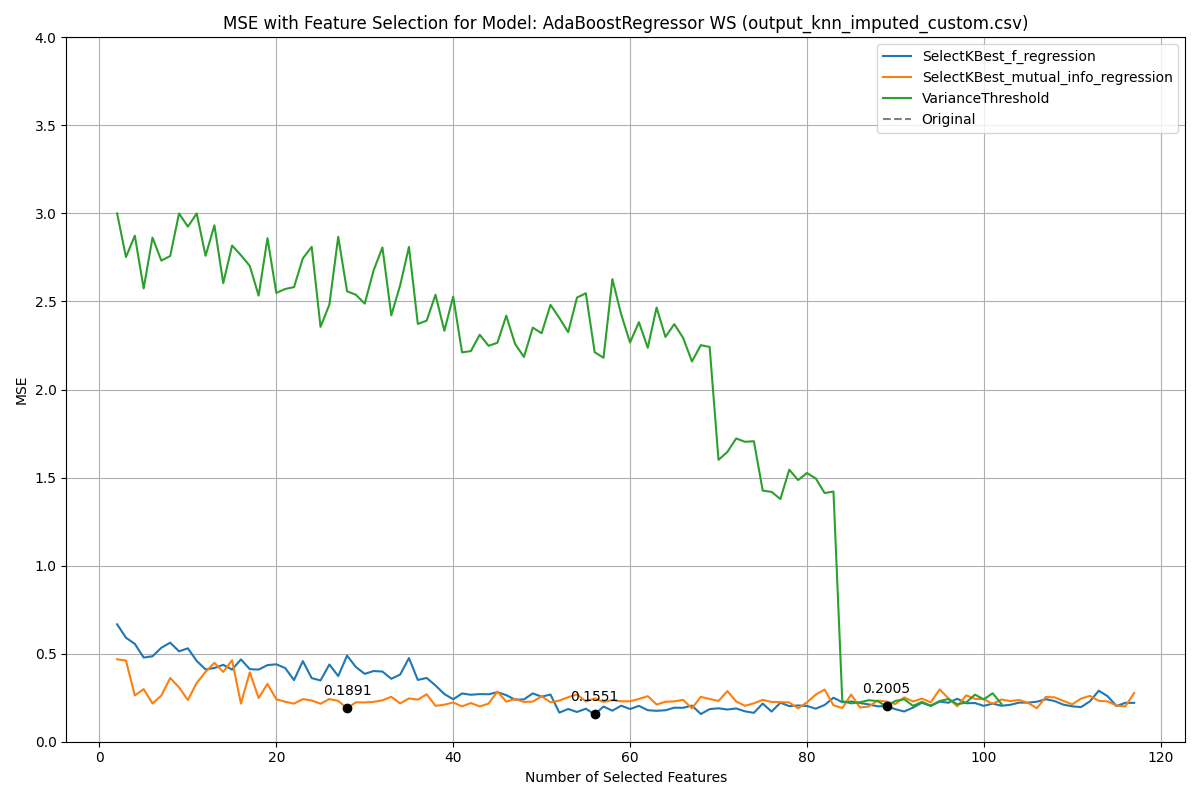
\includegraphics[width=1\linewidth]{reg_section_all/feature_selection_WS_non_norm.png}
    \caption{WS \ac{NNorm} Feature Reduction}
    \label{reg_all_fig:featred_Ex}
\end{figure}
In this figure, we can observe that both \ac{SKB} quickly found the most important features while \ac{VT} did not.
This pattern is repeated for all \ac{EFs} using any \ac{NNorm}, \ac{Norm} or \ac{PNorm}.


Using the top five models, Table \ref{reg_all_tab:summary_mse_features} show our models with ensemble learning.
\begin{table}
\centering
\begin{tabular}{|c||c|p{2.5cm}||c|p{2.5cm}||c|p{2.5cm}|}
\hline
\multirow{2}{*}{\textbf{Feature}} & \multicolumn{2}{c||}{\textbf{\ac{NNorm}}} & \multicolumn{2}{c||}{\textbf{Norm}} & \multicolumn{2}{c|}{\textbf{\ac{PNorm}}} \\
\cline{2-7}
 & \textbf{MSE} & \textbf{Features} & \textbf{MSE} & \textbf{Features} & \textbf{MSE} & \textbf{Features} \\
\hline
PR & 0.3807 & F43, F44, F45 & 0.6054 & F43, F44, F45 & 0.4887 & F43, F44, F45, FedClass \\
\hline
SR & 0.7661 & F24, F28, F29, F31, F43, F44 & 1.2888 & F24, F28, F29, F31, F43, F44 & 0.8795 & F24, F28, F29, F44 \\
\hline
NR & 0.2617 & F24, F43, F44, F45, ProvClass & 0.5116 & F24, F43, F44, F45, ProvClass & 0.7226 & F23, F24, F43, F44, F45, ProvClass \\
\hline
WS & 0.2692 & F22, F24, F28, F31, F43 & 0.5371 & F22, F24, F28, F31, F43 & 0.4695 & F22, F24, F31, F43 \\
\hline
SFST & 0.2988 & F30, F43, F44, F45, F46 & 0.5026 & F30, F43, F44, F45, F46 & 0.4920 & F30, F43, F44, F45, F46 \\
\hline
PR Benefit & 1.2746 & F14, F41, F43, OF19 & 1.3957 & F14, F41, F43, OF19 & 1.3258 & F14, F41, F43, F46, OF19 \\
\hline
SR Benefit & 0.4994 & F41, OF19, OF20, OF21 & 0.4863 & F41, OF19, OF20, OF21 & 2.1352 & F14, F41, OF19, OF20, OF21 \\
\hline
NR Benefit & 3.0567 & F14, F41, OF10, OF19, OF9 & 3.5417 & F14, F41, OF10, OF19, OF9 & 3.7400 & F14, OF10, OF19, OF9 \\
\hline
WS Benefit & 0.7557 & F51, F65, OF17, OF23, OF24 & 0.7679 & F51, F65, OF17, OF23, OF24 & 0.8649 & F51, Hydrogeo., OF17, OF23, OF24 \\
\hline
SFST Benefit & 1.1563 & F1, F23, F43, F44, F45, F46 & 2.2367 & F1, F23, F43, F44, F45, F46 & 2.3455 & F1, F23, F43, F44, F46 \\
\hline
\end{tabular}
\caption{Ensemble Learning MSE and Features Used for Non-Normalized, Normalized and Pre-Normalized Data}
\label{reg_all_tab:summary_mse_features}
\end{table}



In this table, we present each \ac{NNorm}, \ac{Norm} and \ac{PNorm} with the MSE achieved and features used for ensemble learning.
Overall, ensemble learning did not increase our performance significantly.
Using \ac{NNorm}, \ac{SR} Benefit was reduced to 0.4994 using ensemble learning compared to 0.6983 using the top model.
Similarly, \ac{PNorm} did not have a significant advantage using the ensemble learning approach.
Furthermore, ensemble learning increased the number of features used to achieve similar or worse results.
For these reason, we assume ensemble learning to not be effective for regression for this project at this time.
Further data in our training sequence could make ensemble learning beneficial.



Figure \ref{reg_all_fig:ws_featred_big} show a graph the predictions of one of our best results, \ac{SR}.

\begin{figure}
    \centering
    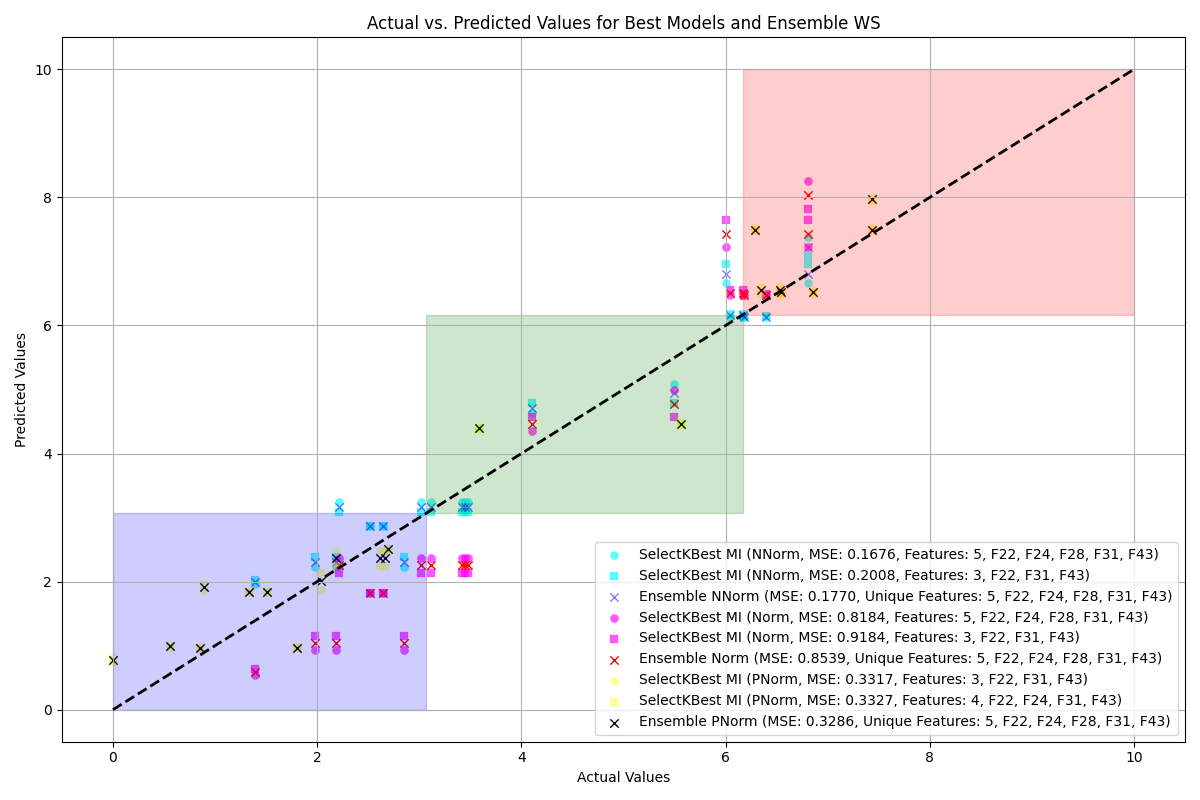
\includegraphics[width=1\linewidth]{reg_section_all/featred_ensemble_learning/actual_vs_predicted_best_feature_selection_and_ensemble_WS_10.png}
    \caption{SR \ac{NNorm} Feature Reduction}
    \label{reg_all_fig:ws_featred_big}
\end{figure}
In this figure, the top two models and our ensemble learning for our three datasets (\ac{NNorm}, \ac{Norm}, \ac{PNorm}) are presented.
In this figure, the classes are presented with blue, green and red squares for lower, moderate and higher ratings.
We can observe how the normalization has an important effect on the results when comparing \ac{NNorm} against \ac{Norm} and \ac{PNorm}.
\ac{NNorm} seems to mostly be concentrated in the moderate class while \ac{Norm} and \ac{PNorm} are more evenly spread out.
It also demonstrates our initial hypothesis on the reason why \ac{NNorm} achieves a lower MSE than\ac{Norm}and \ac{PNorm}.
\ac{NNorm} can cluster the prediction closely together since the range is smaller.
Nonetheless, both \ac{Norm} and \ac{PNorm} have achieved good results with most sites being in the correct class.
Figures \ref{reg_all_fig:pr_featred} to \ref{reg_all_fig:sfst_ben_featred} in the annex show the graphs for all \ac{EF}s.
These figure also demonstrate the difference in results with some \ac{EF}s performing very well, such as \ac{WS} while others, such as \ac{SFST} Benefit, did not.
However, most of our \ac{EF}s achieved impressive results and were able to converge.

To confirm our results, we propose class grouping to compare the results with classification.
We use the lower and higher boundaries presented in section \ref{sec:data} to classify the results.
We present an overview of all three data normalization (\ac{NNorm}, \ac{Norm}, \ac{PNorm}) in table \ref{reg_all_tab:summary_grouping}.
We compared the class grouping using the same boundaries for all three data normalization.
Meaning the non-normalized results use the same classes as the normalized results.
This was done in order to compare the results against each other.

\begin{table}[H]
\centering
\begin{tabular}{|c||c|c||c|c||c|c|}
\hline
\multirow{2}{*}{\textbf{Function}} & \multicolumn{2}{c||}{\textbf{\ac{NNorm}}} & \multicolumn{2}{c||}{\textbf{Norm}} & \multicolumn{2}{c|}{\textbf{\ac{PNorm}}} \\
\cline{2-7}
 & \textbf{Overall} & \textbf{Ensemble} & \textbf{Overall} & \textbf{Ensemble} & \textbf{Overall} & \textbf{Ensemble} \\
\hline
PR & 88.10\% & 90.48\% & 76.19\% & 76.19\% & 78.57\% & 76.19\% \\
\hline
SR & 80.95\% & 88.10\% & 85.71\% & 85.71\% & 85.71\% & 83.33\% \\
\hline
NR & 85.71\% & 85.71\% & 85.71\% & 71.43\% & 88.10\% & 76.19\% \\
\hline
WS & 85.71\% & 73.81\% & 90.48\% & 90.48\% & 90.48\% & 90.48\% \\
\hline
SFST & 90.48\% & 90.48\% & 88.10\% & 88.10\% & 88.10\% & 88.10\% \\
\hline

PR Benefit & 80.95\% & 80.95\% & 85.71\% & 90.48\% & 90.48\% & 90.48\% \\
\hline
SR Benefit & 95.24\% & 92.86\% & 92.86\% & 92.86\% & 95.24\% & 90.48\% \\
\hline
NR Benefit & 90.48\% & 92.86\% & 78.57\% & 83.33\% & 92.86\% & 92.86\% \\
\hline
WS Benefit & 78.57\% & 78.57\% & 80.95\% & 80.95\% & 80.95\% & 83.33\% \\
\hline
SFST Benefit & 83.33\% & 83.33\% & 80.95\% & 80.95\% & 83.33\% & 83.33\% \\
\hline
\end{tabular}
\caption{Summary of Overall and Ensemble Accuracy for Non-Normalized, Normalized and Pre-Normalized Data for Class Grouping}
\label{reg_all_tab:summary_grouping}
\end{table}



When looking at the summary in table \ref{reg_all_tab:summary_grouping}, \ac{PNorm} seems to be the most promising normalization method.
In fact, \ac{NNorm} achieved an accuracy of 87.38\%, \ac{Norm} achieved 84.99\% and \ac{PNorm} achieved 87.62\%.
\ac{NNorm} achieving similar classification results as \ac{PNorm} is unexpected.
Initially we assumed \ac{NNorm} would perform the worst since it was not normalized with the classification bounds.
Nonetheless, it achieved very impressive results with a classification range from 85.71\% to 97.62\%.
\ac{PNorm} achieved a larger range from 78.57\% to a maximum of 95.24\%.
More impressive is the possibility of \ac{NNorm} to classify \ac{NR} with an accuracy of 90.48\% compared to 78.57\% using \ac{PNorm}.
When looking at the global accuracy, meaning the highest for each \ac{EF}, we achieved an overall accuracy of 89.53\%.


Table \ref{reg_all_tab:best} shows the best model for each \ac{EF} with the MSE, overall accuracy and features used.

\begin{table}[H]
\centering
\begin{tabular}{|c|p{3cm}|c|c|c|c|c|}
\hline
\textbf{Function} & \textbf{Model/Data} & \textbf{MSE} & \textbf{Accuracy} & \textbf{Features} & \textbf{Figures}  \\
\hline
 PR & \ac{NNorm}, Ensemble & 0.3807 & 90.48\% & F43, F44, F45 & \ref{reg_all_fig:pr_featred} \\
\hline
 SR & \ac{PNorm}, AdaBoost, KNN & 0.8303 & 88.10\% & F24, F28, F29, F44 & \ref{reg_all_fig:sr_featred} \\
\hline
 NR & \ac{PNorm}, AdaBoost, KNN & 0.7361 & 85.71\% & F24, F43, F44, F45 & \ref{reg_all_fig:nr_featred} \\
\hline
 WS & \ac{PNorm}, AdaBoost, Custom & 0.4642 & 90.48\% & F22, F31, F43 & \ref{reg_all_fig:ws_featred}\\
\hline
 SFST &  \ac{PNorm}, AdaBoost, Custom & 0.5688 & 88.10\% &  F43, F44 & \ref{reg_all_fig:sfst_featred}\\
\hline
 PR Benefit & \ac{PNorm}, MLP, FFill & 1.3627 & 90.48\% & F14, F41, F43, OF19 & \ref{reg_all_fig:pr_ben_featred}\\
\hline
SR Benefit & \ac{PNorm}, AdaBoost, FFill & 2.0620 & 95.24\% &  F41, OF19, OF21& \ref{reg_all_fig:sr_ben_featred}\\
\hline
 NR Benefit & \ac{PNorm}, MLP, KNN & 3.4702 & 92.86\% & F14, OF9, OF10, OF19 & \ref{reg_all_fig:nr_ben_featred}\\
\hline
 WS Benefit & \ac{PNorm}, AdaBoost, Mean & 0.9022 & 80.95\% & Hydrogeo., OF17, OF23, OF24  & \ref{reg_all_fig:ws_ben_featred}\\
\hline
 SFST Benefit & \ac{PNorm}, AdaBoost, Iterative & 2.3641 & 83.33\% & F43, F44 & \ref{reg_all_fig:sfst_ben_featred} \\
\hline
\end{tabular}
\caption{Best Model Results for All Features}
\label{reg_all_tab:best}
\end{table}

In this table, we can see that \ac{PNorm} was the most efficient data normalization technique while AdaBoost was the best algorithm.






\subsection{Specific Features}
\subsubsection{Training Results}

Table \ref{reg_spec_tab:mse_summary} shows a summary of our training results.
In order, this table shows \ac{NNorm}, \ac{Norm} and \ac{PNorm} for all \ac{EF}s functions and benefits.
With the exception of \ac{SFST} Benefit, all \ac{EF}s performed well and achieved good performance.
In fact, we achieved MSE ranging from 0.01 to 0.16 when excluding \ac{SFST} Benefit, which achieved 1.66.
When comparing the data normalization, \ac{NNorm} achieved the overall best performance, closely followed by \ac{PNorm}.
\ac{Norm} achieved a higher MSE than \ac{NNorm} and \ac{PNorm} for most \ac{EF}s, with a few exceptions.
Certain \ac{EF}s achieved a better MSE using \ac{NNorm}, while others performed better using \ac{PNorm}.
\ac{PR} Benefit excelled using any normalization and achieved an MSE of 0.01 across all normalization techniques.
Overall, the Benefit scores for \ac{NR}, \ac{SR} and \ac{PR} achieved a better MSE than their function counterparts.
When compared against Table \ref{reg_all_tab:mse_summary}, which uses all features, we achieved significantly better results.

When comparing all \ac{EF}s, we achieved an average MSE of 0.359, 0.520 and 0.402 for all features, while specific features achieved 0.295, 0.614 and 0.960 for \ac{NNorm}, \ac{Norm} and \ac{PNorm}, respectively.
However, due to \ac{SFST} Benefit achieving an abnormally high MSE, we verified the results using the median.
In terms of median, we achieved 0.22, 0.45 and 0.31 using all features, while we achieved 0.10, 0.19 and 0.24 using specific features.
When removing \ac{SFST} Benefit, we achieved averages of 0.312, 0.469 and 0.367 using all features, while specific features achieved 0.142, 0.211 and 0.137.
These results demonstrate two things: first, they show how a single outlier can skew the perception of our results.
At first glance, using the averages, all features performed better than specific features.
However, when removing the outlier, the specific features significantly outperformed all features.
These results also show that \ac{SFST} Benefit is missing important features in the specific dataset to infer its score.
Our specific features achieved lower results for both classification and regression for \ac{SFST} Benefit.
This highlights our reasoning for using all features rather than only specific features.
The \ac{WESP-AC} may only require specific features to calculate the score, while \ac{ML} may require different ones.
Nonetheless, our results using only specific features are highly promising, with most \ac{EF}s achieving low MSE.

\begin{table}[H]
\centering
\begin{tabular}{|c|c|c|c|}
\hline
\textbf{Feature} & \textbf{Non-Normalized MSE} & \textbf{Normalized MSE} & \textbf{Pre-Normalized MSE} \\
\hline
NR & 0.15 & 0.43 & 0.24 \\
\hline
PR & 0.11 & 0.18 & 0.24 \\
\hline
SR & 0.08 & 0.13 & 0.27 \\
\hline
SFST & 0.16 & 0.26 & 0.20 \\
\hline
WS & 0.10 & 0.19 & 0.08 \\
\hline
NR Benefit & 0.08 & 0.09 & 0.07 \\
\hline
PR Benefit & 0.01 & 0.01 & 0.01 \\
\hline
SR Benefit & 0.07 & 0.09 & 0.01 \\
\hline
SFST Benefit & 1.66 & 3.22 & 4.37 \\
\hline
WS Benefit & 0.53 & 0.54 & 0.11 \\
\hline
\end{tabular}
\caption{Summary of Best MSE for Non-Normalized, Normalized and Pre-Normalized Data}
\label{reg_spec_tab:mse_summary}
\end{table}

In the annex, figure \ref{reg_spec_tab:norm_mse} shows the full results for \ac{NNorm} and \ac{Norm}, while figure \ref{reg_spec_tab:pre_norm_mse} shows \ac{PNorm}.
In these tables, we show which model and data filling method the results were achieved with.
The AdaBoost regressor achieved the overall best results and was used for most \ac{EF}s.
Most filling methods performed similarly, with no clear benefit of using a specific one.
However, our custom filling was the most popular, with seven appearances, while mean, iterative, or KNN appeared three times each.
We assume our custom method, which used -1, enabled our models to know the value was missing.
Using methods that infer missing values may confuse the model by using wrong values, while using -1 may enable the model to infer it by itself.
In future iterations of our work, it could be interesting to use different custom methods.
It would also be interesting to use different filling methods for different features.
Features that are only missing sporadically could use methods such as iterative, while mostly missing features could use our custom approach.

We also implemented ensemble learning using the specific features dataset.
Table \ref{reg_spec_tab:ensemble} shows the results of ensemble learning.
In this table, each normalization method is presented with and without ensemble learning.
Similar to previous sections, ensemble learning did not seem to benefit the models.
In fact, in most instances, the MSE was increased when using ensemble learning.
\ac{Norm} benefited from ensemble learning the most, with some \ac{EF}s achieving lower MSE with ensemble learning.
However, the reduction in MSE is not significant since it is only by a few units.

\begin{table}[H]
\centering
\begin{tabular}{|c||c|c|c||c|c|c|}
\hline
\multirow{2}{*}{\textbf{Feature}} & \multicolumn{3}{c||}{\textbf{Specific}} & \multicolumn{3}{c|}{\textbf{Ensemble}} \\
\cline{2-7}
 & \textbf{Non-Norm} & \textbf{Norm} & \textbf{Pre-Norm} & \textbf{Non-Norm} & \textbf{Norm} & \textbf{Pre-Norm} \\
\hline
PR &  0.11 & 0.18 & 0.24 & 0.10 & 0.16 & 0.24 \\
\hline
NR &  0.15 & 0.43 & 0.24 & 0.14 & 0.40 & 0.22 \\
\hline
SR &  0.08 & 0.13 & 0.27 & 0.07 & 0.11 & 0.18 \\
\hline
WS & 0.10 & 0.19 & 0.08 & 0.06 & 0.11 & 0.13 \\
\hline
SFST &  0.16 & 0.26 & 0.20 & 0.17 & 0.29 & 0.20 \\
\hline
PR Benefit & 0.01 & 0.01 & 0.01 & 0.23 & 0.01 & 0.0 \\
\hline
NR Benefit &  0.08 & 0.09 & 0.07 & 0.11 & 0.12 & 0.04 \\
\hline
SR Benefit &  0.07 & 0.09 & 0.01 & 0.12 & 0.09 & 0.02 \\
\hline
WS Benefit &  0.53 & 0.54 & 0.11 & 0.54 & 0.55 & 0.09 \\
\hline
SFST Benefit & 1.66 & 3.22 & 4.37 & 1.90 & 3.61 & 4.40 \\
\hline
\end{tabular}
\caption{Ensemble Learning for Specific Features}
\label{reg_spec_tab:ensemble}
\end{table}

In the annex, figures \ref{reg_spec_fig:pr_ensemble} to \ref{reg_spec_fig:sfst_ben_ensemble} show the predictions with the classes.
When looking at the overall behavior of these figures, we can see that all three normalizations performed well.
\ac{PNorm} achieved better results than \ac{Norm} as expected, with \ac{PNorm} being closer to the actual values.
\ac{NNorm} achieved better results than \ac{PNorm} for functions, while it achieved slightly lower results for benefits.
Figure \ref{reg_spec_fig:ws_ensemble_big} below shows the ensemble learning graph for \ac{WS}.
In this figure, we can see how well our algorithms performed using any normalization.

\begin{figure}[h]
    \centering
    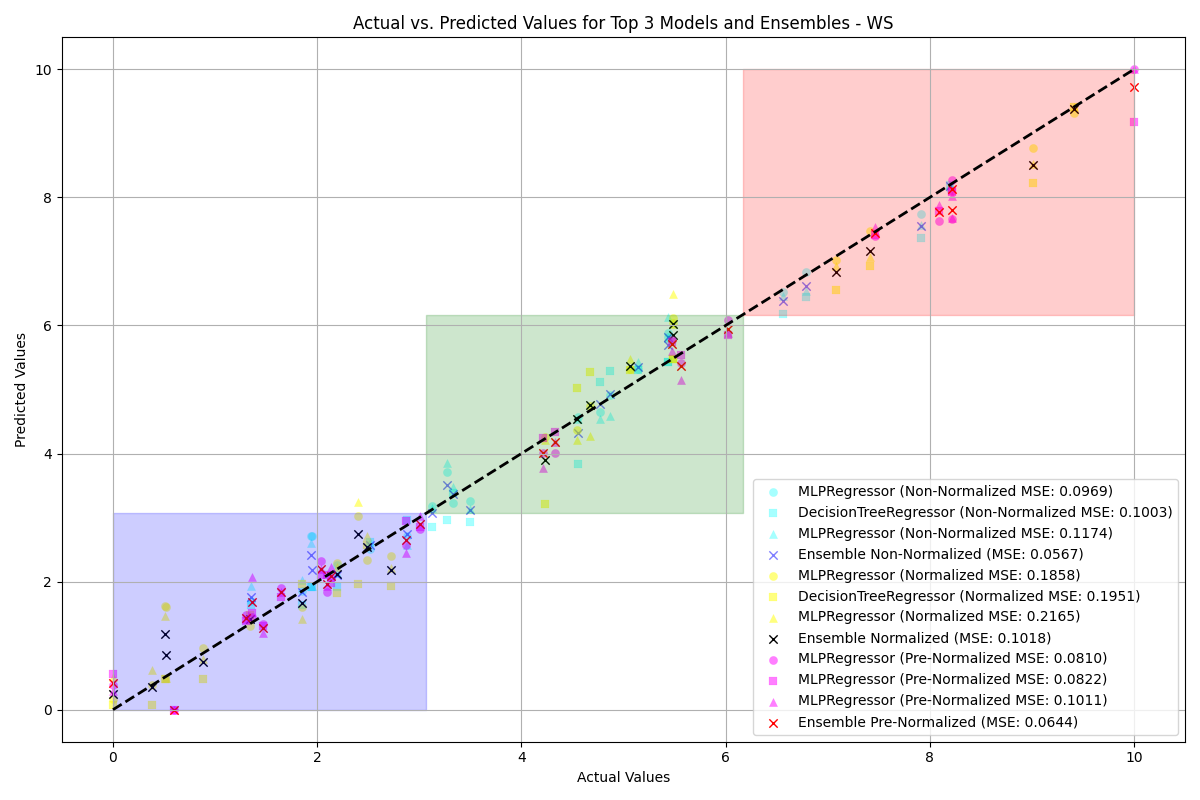
\includegraphics[width=0.95\linewidth]{reg_section_specific/ensemble_learning/actual_vs_predicted_top_3_models_and_ensembles_WS.png}
    \caption{WS Graphs Specific Features}
    \label{reg_spec_fig:ws_ensemble_big}
\end{figure}

Most sites, using\ac{Norm}or \ac{PNorm}, were within an MSE score of one or less.
This figure also demonstrates how good our regression predictions can be for class grouping.
Table \ref{reg_spec_tab:summary_class_grouping} shows the class grouping, while tables \ref{reg_spec_tab:non_norm_accuracy}, \ref{reg_spec_tab:norm_accuracy} and \ref{reg_spec_tab:pre_norm_accuracy} show the detailed results.

\begin{table}[H]
\centering
\begin{tabular}{|c||c|c||c|c||c|c|}
\hline
\multirow{2}{*}{\textbf{Function}} & \multicolumn{2}{c||}{\textbf{\ac{NNorm}}} & \multicolumn{2}{c||}{\textbf{Norm}} & \multicolumn{2}{c|}{\textbf{\ac{PNorm}}} \\
\cline{2-7}
 & \textbf{Overall} & \textbf{Ensemble} & \textbf{Overall} & \textbf{Ensemble} & \textbf{Overall} & \textbf{Ensemble} \\
\hline
PR & 90.48\% & 92.86\% & 78.57\% & 76.19\% & 90.48\% & 90.48\% \\
\hline
SR & 85.71\% & 85.71\% & 80.95\% & 76.19\% & 92.86\% & 92.86\% \\
\hline
NR & 88.10\% & 85.71\% & 80.95\% & 71.43\% & 100.00\% & 95.24\% \\
\hline
WS & 90.48\% & 90.48\% & 97.62\% & 97.62\% & 95.24\% & 90.48\% \\
\hline
SFST & 90.48\% & 90.48\% & 88.10\% & 88.10\% & 97.62\% & 97.62\% \\
\hline
PR Benefit & 92.86\% & 90.48\% & 92.86\% & 92.86\% & 88.10\% & 88.10\% \\
\hline
SR Benefit & 92.86\% & 85.71\% & 90.48\% & 83.33\% & 100.00\% & 100.00\% \\
\hline
NR Benefit & 92.86\% & 92.86\% & 92.86\% & 92.86\% & 88.10\% & 88.10\% \\
\hline
WS Benefit & 78.57\% & 78.57\% & 80.95\% & 85.71\% & 92.86\% & 90.48\% \\
\hline
SFST Benefit & 71.43\% & 66.67\% & 52.38\% & 52.38\% & 50.00\% & 52.38\% \\
\hline
\end{tabular}
\caption{Summary of Overall and Ensemble Accuracy for Non-Normalized (\ac{NNorm}), Normalized (Norm) and Pre-Normalized (\ac{PNorm}) Data for Class Grouping}
\label{reg_spec_tab:summary_class_grouping}
\end{table}

The overall results in Table \ref{reg_spec_tab:summary_class_grouping} show promising results.
\ac{NNorm} performed very well when considering it does not normalize the data and the boundaries were generated using the normalization sites.
In fact, it achieved better results on most \ac{EF}s than the \ac{Norm} data.
\ac{PNorm} achieved the best results for seven of the ten \ac{EF}s, with the remaining three being close.
In fact, \ac{NNorm}, \ac{Norm} and \ac{PNorm} respectively achieved an average overall accuracy of 87.083\%, 83.472\% and 89.426\%.
Impressively, \ac{NNorm} achieved a classification accuracy of 71.43\% on \ac{SFST} Benefit compared to the second best of 52.38\%.
When excluding \ac{SFST} Benefit, our data normalization techniques achieved 89.155\%, 87.038\% and 93.925\% for \ac{NNorm}, \ac{Norm} and \ac{PNorm}.
These results are similar to using classification directly on the specific features.
However, with regression, we are able to directly predict the score, which is highly beneficial.

\subsubsection{Feature Reduction}

Using the best performing model for each normalization technique, we performed feature reduction.
We used the same three techniques as in the previous sections.
Table \ref{reg_spec_tab:featred_res} shows the best models with a maximum of five features.

\begin{table}[H]
\centering
\begin{tabular}{|c|c|c|p{2.5cm}|c|p{2.5cm}|}
\hline
\textbf{\ac{EF}} & \textbf{\ac{NNorm}} & \textbf{Norm} & \textbf{Features} & \textbf{\ac{PNorm}} & \textbf{Features} \\
\hline
PR & 0.2463 & 0.3916 & F24, F28, F43, F44, F45 & 1.0651 & F28, F43, F44, F45 \\
\hline
SR & 0.5499 & 0.9251 & F28, F29, F31, F43, F44 & 1.3284 & F28, F31, F44 \\
\hline
NR & 0.2879 & 0.7066 & F1, F24, F43, F44, F45 & 0.0850 & F43, F44 \\
\hline
WS & 0.0838 & 0.1665 & F22, F28, F31, F43 & 0.8815 & F22, F28, F31, F43, F44 \\
\hline
SFST & 0.2208 & 0.3715 & F1, F14, F24, F43 & 0.6496 & F1, F43 \\
\hline
PR Benefit & 0.7844 & 0.8554 & F41, OF19, OF20, OF21, OF24 & 0.3265 & F41, OF19, OF20, OF21, OF22 \\
\hline
NR Benefit & 2.6496 & 3.0701 & F41, OF10, OF19, OF9 & 0.8918 & F41, OF10, OF19, OF21, OF9 \\
\hline
SR Benefit & 2.5425 & 2.3806 & F41, OF19 & 0.1807 &  F41, OF19, OF21 \\
\hline
WS Benefit & 0.6022 & 0.6119 & F51, OF17, OF18, OF23, OF24 & 2.1603 & F51, OF17, OF23, OF24, OF8 \\
\hline
SFST Benefit & 2.2402 & 4.3334 & OF22, OF25, OF28 & 9.8386 & F50, OF22, OF25, OF28 \\
\hline
\end{tabular}
\caption{Best MSE with Corresponding Features}
\label{reg_spec_tab:featred_res}
\end{table}

In this table, we show each \ac{EF} with both the \ac{NNorm} and \ac{Norm} MSE with their respective features, while \ac{PNorm} shows the same.
In comparison with using all specific features on \ac{FS}, our reduced features achieved slightly higher MSEs.
Our Benefit scores performed poorly using reduced features.
Using \ac{NNorm}, \ac{PR} Benefit increased from 0.01 to 0.7844, while \ac{NR} Benefit increased to 2.6496 from 0.08.
Compared to feature reduction using all features, reduced specific features often achieved a higher MSE.
In rare cases the MSE was decreased such as with \ac{WS} using \ac{NNorm}, D2 achieved an MSE of 0.0838 using four features, while using D4 it achieved 0.2692 with four features.
This could be caused by the model having too much data, which hinders its ability to learn.
Nonetheless, our overall results demonstrate that using specific features can be beneficial over using all features.

Our ensemble learning results did not increase our performance and often increased the MSE.
In the annex, we show our ensemble learning results in figures \ref{reg_spec_fig:pr_featred} to \ref{reg_spec_fig:sfst_ben_featred}.
They show our validation predictions for the top two models and the ensemble approach for all three normalizations.
A glaring issue is the normalized non-normalized predictions, which seem to have a larger error margin.
This makes sense since they are the \ac{NNorm} predictions scaled, which means the errors are also scaled.
Nonetheless, we achieved good grouping, such as in figure \ref{reg_spec_fig:nr_featred_big}, where three distinct clusters can be seen for\ac{Norm}and \ac{PNorm}.
A cluster near the lower-moderate boundary, near the moderate-higher boundary and in the higher class can be seen.
This demonstrates that our approach can cluster regression predictions into classes well.

\begin{figure}
    \centering
    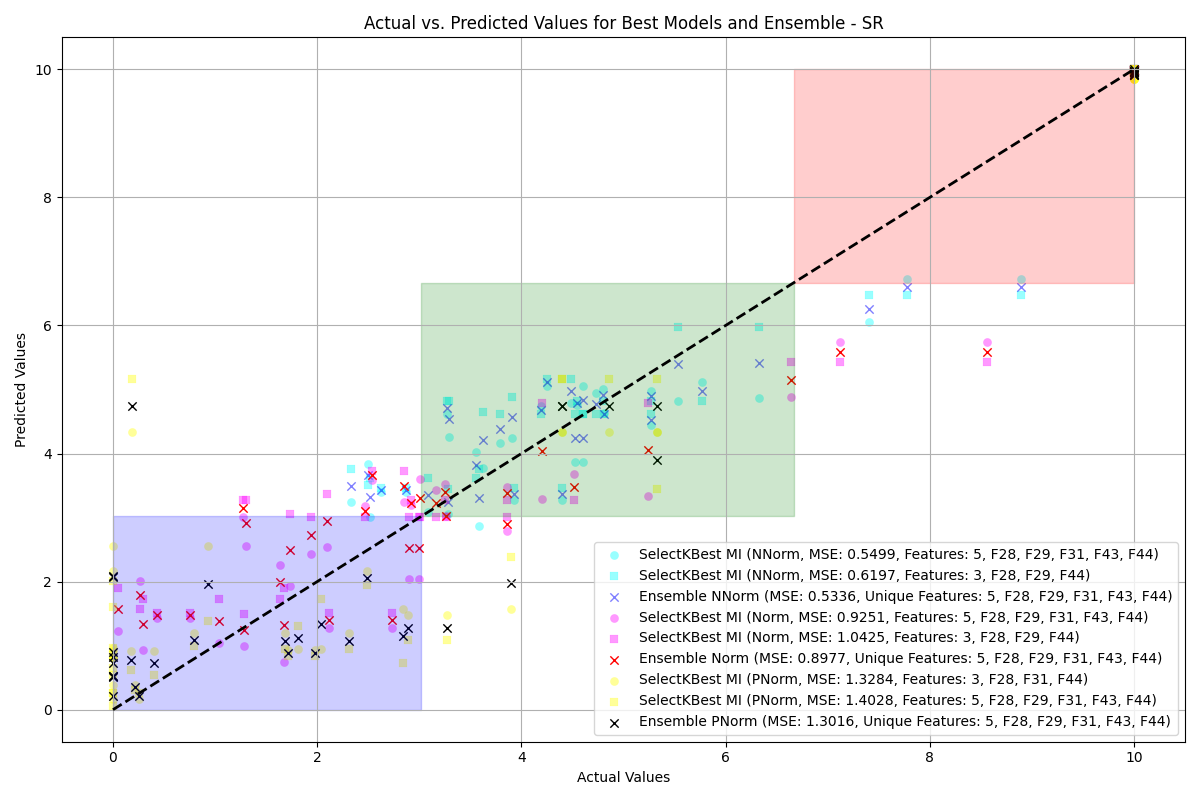
\includegraphics[width=1\linewidth]{reg_section_specific/featred_ensemble_learning/actual_vs_predicted_best_feature_selection_and_ensemble_SR_10.png}
    \caption{NR Graphs Specific Features}
    \label{reg_spec_fig:nr_featred_big}
\end{figure}

These results are confirmed in table \ref{reg_spec_tab:summary_grouping}, which shows a summary of our class grouping.

\begin{table}[H]
\centering
\begin{tabular}{|c||c|c||c|c||c|c|}
\hline
\multirow{2}{*}{\textbf{Function}} & \multicolumn{2}{c||}{\textbf{\ac{NNorm}}} & \multicolumn{2}{c||}{\textbf{Norm}} & \multicolumn{2}{c|}{\textbf{\ac{PNorm}}} \\
\cline{2-7}
 & \textbf{Overall} & \textbf{Ensemble} & \textbf{Overall} & \textbf{Ensemble} & \textbf{Overall} & \textbf{Ensemble} \\
\hline
WS & 90.48\% & 90.48\% & 97.62\% & 97.62\% & 95.24\% & 90.48\% \\
\hline
PR & 90.48\% & 92.86\% & 78.57\% & 76.19\% & 90.48\% & 90.48\% \\
\hline
NR & 88.10\% & 85.71\% & 80.95\% & 71.43\% & 100.00\% & 95.24\% \\
\hline
SR & 85.71\% & 85.71\% & 80.95\% & 76.19\% & 92.86\% & 92.86\% \\
\hline
SFST & 90.48\% & 90.48\% & 88.10\% & 88.10\% & 97.62\% & 97.62\% \\
\hline
PR Benefit & 92.86\% & 90.48\% & 92.86\% & 92.86\% & 88.10\% & 88.10\% \\
\hline
SR Benefit & 92.86\% & 85.71\% & 90.48\% & 83.33\% & 100.00\% & 100.00\% \\
\hline
NR Benefit & 92.86\% & 92.86\% & 92.86\% & 92.86\% & 88.10\% & 88.10\% \\
\hline
WS Benefit & 78.57\% & 78.57\% & 80.95\% & 85.71\% & 92.86\% & 90.48\% \\
\hline
SFST Benefit & 71.43\% & 66.67\% & 52.38\% & 54.76\% & 50.00\% & 52.38\% \\
\hline
\end{tabular}
\caption{Summary of Overall and Ensemble Accuracy for Non-Normalized (\ac{NNorm}), Normalized (Norm) and Pre-Normalized (\ac{PNorm}) Data for Class Grouping}
\label{reg_spec_tab:summary_grouping}
\end{table}

In this table, we show the overall classification accuracy for each normalization for both the top approach and ensemble.
\ac{PNorm} achieved the overall best accuracy of 89.39\%, while \ac{NNorm} and \ac{Norm} achieved 87.38\% and 83.33\%, respectively.
Compared to using all specific features, we slightly decreased the performance.
Using all features, we achieved 89.426\%, 87.083\% and 83.472\%, while we achieved 89.39\%, 87.38\% and 83.33\% for \ac{PNorm}, \ac{NNorm} and Norm, respectively.
To handle the \ac{SFST} Benefit outlier problem, we compared the averages without it.
\ac{PNorm} achieved the best at 92.41\%, while \ac{NNorm} and \ac{Norm} achieved 89.16\% and 87.37\%, respectively.
These results were comparable to using all features, which achieved 93.925\%, 89.155\% and 87.138\%.
However, due to the significant decrease in features used, using reduced specific features achieved impressive results.
We achieved similar results on all \ac{EF}s while using a portion of the specific features.

Tables \ref{reg_spec_tab:featred_non_norm_accuracy}, \ref{reg_spec_tab:featred_post_norm_accuracy} and \ref{reg_spec_tab:featred_norm_accuracy} show detailed results.
In these tables, we show the lower, moderate and higher accuracies of \ac{NNorm}, \ac{Norm} and \ac{PNorm}, respectively.
These tables provide us with information such as a lack of sites in the validation dataset.
Having an equal number of sites for each rating would be beneficial.

Table \ref{reg_spec_tab:best} shows the best results for the Specific Features dataset.

\begin{table}[H]
\centering
\begin{tabular}{|c|p{3cm}|c|c|p{3cm}|c|}
\hline
\textbf{Function} & \textbf{Model/Data} & \textbf{MSE} & \textbf{Accuracy} & \textbf{Features} & \textbf{Figures}  \\
\hline
 PR & \ac{PNorm}, AdaBoost, Iterative & 1.0651 & 90.48\% & F28, F43, F44, F5 &\ref{reg_spec_fig:pr_featred} \\
\hline
 SR & \ac{PNorm}, MLP, Custom & 1.3284 & 92.86\% & F28, F31, F44 & \ref{reg_spec_fig:sr_featred} \\
\hline
 NR & \ac{PNorm}, AdaBoost, Iterative & 0.0850 & 100.00\% & F43, F44 & \ref{reg_spec_fig:nr_featred} \\
\hline
 WS & Norm, MLP, Mode & 0.1665 & 97.62\% & F22, F28, F31, F43 & \ref{reg_spec_fig:ws_featred}\\
\hline
 SFST & \ac{PNorm}, AdaBoost, Mean & 0.6496 & 97.62\% & F1, F43 & \ref{reg_spec_fig:sfst_featred}\\
\hline
 PR Benefit & \ac{PNorm}, MLP, Median & 0.3265 & 92.86\% & F41, OF19, OF20, OF21, OF22 & \ref{reg_spec_fig:pr_ben_featred}\\
\hline
SR Benefit & \ac{PNorm}, DecisionTree, Median & 0.1807 & 100.00\% & F41, OF19, OF21 & \ref{reg_spec_fig:sr_ben_featred}\\
\hline
 NR Benefit & \ac{PNorm}, MLP, Custom & 0.8918 & 92.86\% & F41, OF9, OF10, OF19, OF21 & \ref{reg_spec_fig:nr_ben_featred}\\
\hline
 WS Benefit & \ac{PNorm}, DecisionTree, Mean & 2.1603 & 92.86\% & F51, OF8, OF17, OF23, OF24 & \ref{reg_spec_fig:ws_ben_featred}\\
\hline
 SFST Benefit & \ac{NNorm}, RANSAC, Interpolated & 2.2402 & 71.43\% & OF22, OF25, OF28 & \ref{reg_spec_fig:sfst_ben_featred} \\
\hline
\end{tabular}
\caption{Best Models Using Specific Features}
\label{reg_spec_tab:best}
\end{table}

In this table, we present which model for each \ac{EF} achieved the best MSE and accuracy with reduced features.
Excluding \ac{SFST} Benefit, we achieved a range of accuracies from 90.48\% to 100.00\% using two to five features.
This number of features is a considerable improvement from using all or even just specific features.
\ac{NR}, which usually requires 33 features, was reduced to using only two features to achieve 100.00\% accuracy.
Similarly, \ac{SR} Benefit achieved an accuracy of 100.00\% using only three features.
These results are highly impressive since we only used \~200 sites for training.
However, more training would be required since 100.00\% should not be taken as a perfect model.
Furthermore, using \ac{PNorm} limits our models to use only sites that can be normalized using the same calibration sites.
Our \ac{NNorm} data also achieved good results with slightly lower accuracy with a similar number of features.
These results demonstrate that we can use normalized, non-normalized and pre-normalized results.
Each method has its benefits and can be used for specific situations depending on the requirements.


\subsection{Dataset Comparison}
To more easily compare the differences in results, we present the best-performing models for each \ac{EF} for both classification and regression. The models that achieved the most interesting results are shown in Tables \ref{reg_spec_tab:best} and \ref{reg_all_tab:best}.

\begin{longtable}{|p{3cm}|p{2cm}|p{2cm}|p{2cm}|p{2cm}|p{3cm}|}
\hline
\textbf{Function} & \textbf{MSE All} & \textbf{Acc. All} & \textbf{MSE Specific} & \textbf{Acc. Specific} & \textbf{Features} \\ \hline
\endfirsthead
\hline
\textbf{Function} & \textbf{MSE All} & \textbf{Acc. All} & \textbf{MSE Specific} & \textbf{Acc. Specific} & \textbf{Features} \\ \hline
\endhead

PR & 0.3807 & 90.48\% & 1.0651 & 90.48\% & F28, F43, F44, F45 \\ \hline
SR & 0.8303 & 88.10\% & 1.3284 & 92.86\% & F28, F31, F44 \\ \hline
NR & 0.7361 & 85.71\% & 0.0850 & 100.00\% & F43, F44 \\ \hline
WS & 0.4642 & 90.48\% & 0.1665 & 97.62\% & F22, F28, F31, F43 \\ \hline
SFST & 0.5688 & 88.10\% & 0.6496 & 97.62\% & F1, F43 \\ \hline
PR Benefit & 1.3627 & 90.48\% & 0.3265 & 92.86\% & F41, OF19, OF20, OF21, OF22 \\ \hline
SR Benefit & 2.0620 & 95.24\% & 0.1807 & 100.00\% & F41, OF19, OF21 \\ \hline
NR Benefit & 3.4702 & 92.86\% & 0.8918 & 92.86\% & F41, OF9, OF10, OF19, OF21 \\ \hline
WS Benefit & 0.9022 & 80.95\% & 2.1603 & 92.86\% & F51, OF8, OF17, OF23, OF24 \\ \hline
SFST Benefit & 2.3641 & 83.33\% & 2.2402 & 71.43\% & OF22, OF25, OF28 \\ \hline
\caption{Comparison of Best Model Results Using All and Specific Features}
\label{tab_combined:featred_comparison}
\end{longtable}

Table \ref{tab_combined:featred_comparison} highlights the performance differences between models using all features versus specific features. Notably, the accuracy and MSE for several \acp{EF}, such as \ac{SR} and \ac{SFST} Benefit, show significant variation when using different feature sets. For instance, the \ac{NR} function saw a substantial improvement in accuracy and a lower MSE when using specific features, whereas the \ac{PR} Benefit and \ac{SR} Benefit functions achieved better results with specific features compared to all features.

The performance drop in models using all features for some functions suggests that additional or irrelevant features might have introduced noise, making it harder for the models to learn effectively. On the other hand, the specific feature sets appear to better capture the essential characteristics needed for accurate predictions in certain cases.

This analysis underscores the importance of carefully selecting features based on the specific requirements of each \ac{EF}. In future work, a more detailed investigation into the feature selection process could help to further refine the models and achieve even better results.

Furthermore, the use of different models and data filling methods, as indicated in the table, suggests that certain combinations are more effective for particular \acp{EF}. For instance, the use of AdaBoost with \ac{PNorm} data consistently yielded strong performance across several functions. 

Overall, while the use of all features can sometimes lead to better outcomes, specific features often provide more precise and reliable predictions, particularly when dealing with complex ecological functions.


\clearpage


\section{Detailed Analysis of \ac{EF}s using \ac{ML}}
In this section, we discuss our findings for different \ac{EF}s separately. Table \ref{tab:combined_summary} presents the best results for both classification and regression using all and specific features. 

\begin{longtable}{|p{2cm}|p{1.5cm}|p{1.5cm}|p{3.5cm}|p{1.5cm}|p{3.5cm}|}
\hline
\textbf{Function} & \textbf{Type} & \multicolumn{2}{c|}{\textbf{All Features}} & \multicolumn{2}{c|}{\textbf{Specific Features}} \\
\cline{3-6}
 & & \textbf{Acc.} & \textbf{Features} & \textbf{Acc.} & \textbf{Features} \\
\hline
\endfirsthead

\hline
\textbf{Function} & \textbf{Type} & \multicolumn{2}{c|}{\textbf{All Features}} & \multicolumn{2}{c|}{\textbf{Specific Features}} \\
\cline{3-6}
 & & \textbf{Acc.} & \textbf{Features} & \textbf{Acc.} & \textbf{Features} \\
\hline
\endhead

PR & Class. & 85.71\% & F43, F45 & 85.71\% & F43, F45 \\
\cline{2-6}
 & Reg. & \textbf{90.48\%} & \textbf{F43, F44,} F45 & 90.48\% & F28, F43, F44, F5 \\
\hline
SR & Class. & 80.95\% & Hydrogeo., F24, F29, F43, F44, F45 & 71.42\% & OF22, F35, F43, F45, F49 \\
\cline{2-6}
 & Reg. & 88.10\% & F24, F28, F29, F44 & \textbf{92.86\%} & \textbf{F28, F31, F44} \\
\hline
NR & Class. & 80.95\% & F43, F44 & 80.95\% & F43, F44, F45 \\
\cline{2-6}
 & Reg. & 85.71\% & F24, F43, F44, F45 & \textbf{100.00\%} & \textbf{F43, F44} \\
\hline
WS & Class. & 90.45\% & F43, F46 & 85.71\% & F43, F44 \\
\cline{2-6}
 & Reg. & 90.48\% & F22, F31, F43 & \textbf{97.62\%} &\textbf{ F22, F28, F31, F43} \\
\hline
SFST & Class. & 95.24\% & F43, F44 & 95.24\% & F1, F43 \\
\cline{2-6}
 & Reg. & 88.10\% & F43, F44 &\textbf{ 97.62\%} & \textbf{F1, F43} \\
\hline
PR Benefit & Class. & 90.45\% & F14, F24, F41, F43, F46, F47 & 85.71\% & OF22, F41 \\
\cline{2-6}
 & Reg. & 90.48\% & F14, F41, F43, OF19 & \textbf{92.86\%} & \textbf{F41, OF19, OF20, OF21, OF22 }\\
\hline
SR Benefit & Class. & 100.00\% & OF19, OF21, F41, F43 & 95.24\% & OF19, F41 \\
\cline{2-6}
 & Reg. & 95.24\% & F41, OF19, OF21 & \textbf{100.00\%} & \textbf{F41, OF19, OF21} \\
\hline
NR Benefit & Class. & 90.45\% & MossCover, OF9, OF10, OF19, F1, F14, F41, F43 & 90.48\% & OF9, OF10, OF19, OF21, F41 \\
\cline{2-6}
 & Reg. & \textbf{92.86\%} & \textbf{F14, OF9, OF10, OF19} & 92.86\% & F41, OF9, OF10, OF19, OF21 \\
\hline
WS Benefit & Class. & \textbf{95.24\%} & \textbf{OF17, OF23} & 95.24\% & OF17, OF24, F51 \\
\cline{2-6}
 & Reg. & 80.95\% & Hydrogeo., OF17, OF23, OF24 & 92.86\% & F51, OF8, OF17, OF23, OF24 \\
\hline
SFST Benefit & Class. & 80.95\% &  F43, F44 & 57.14\% & OF22, OF28 \\
\cline{2-6}
 & Reg. & \textbf{83.33\%} & \textbf{F43, F44 }& 71.43\% & OF22, OF25, OF28 \\
\hline
\caption{Combined Summary of Accuracy and Features for Classification and Regression, Including Benefits}
\label{tab:combined_summary}
\end{longtable}

In this table, the most pertinent model for each \ac{EF} is highlighted in bold.
We shoe the classification results for each \ac{EF} for classification and regression with both D2 and D4.

\subsection{PR}
Phosphorus retention is critical for the health and biodiversity of our planet.
It reflects the ability of a wetland to retain phosphorus for long periods.
Agricultural activities can increase the quantity of phosphorus in surrounding areas, negatively impacting wetlands.
Monitoring the phosphorus retention capacity of a wetland provides valuable insights into land management practices.

PR is one of the most demanding \ac{EF}s, requiring 22 features from the \ac{WESP-AC} for the \ac{FS} and 11 for \ac{FS}.
Reducing the number of features needed to evaluate a site could significantly aid researchers.
When analyzing Table \ref{tab:combined_summary}, \ac{PR} shows promising results for \ac{FS}.
Both all features and specific features datasets achieved similar accuracy scores.

In classification, both datasets used F43 and F45, achieving an accuracy of 85.71\%.
For regression, F43, F44 and F45 were utilized to achieve 90.48\%, with specific features requiring the addition of F28.
These features (F43, F44, F45) respectively define the channel connection and outflow duration, outflow confinement and through-flow resistance.
These WESP-AC features impact \ac{PR} by indicating a wetland's ability to retain or drain water.
F28, which measures surface water annual fluctuation, can indicate changes in water level, offering insights into \ac{PR}.
These four features have a significant influence on the results of \ac{PR} \ac{FS}.

Phosphorus retention offers substantial benefits to human populations by maintaining the quality of receiving waters.
PR Benefit evaluates how beneficial a wetland's phosphorus retention is for humans.
A site might be effective at phosphorus retention but not necessarily beneficial to humans and vice versa.

PR Benefit employs 11 features, sharing only one feature with PR: OF22.
This distinction highlights the different focuses of \ac{FS} and \ac{BS}.
The overview table shows that \ac{PR} \ac{BS} required more features than \ac{FS}.
The best-performing model required five features, while \ac{FS} only needed three.

Regression using specific features yielded the best model with an accuracy of 92.86\%, using F41, OF19, OF20, OF21 and OF22.
F41 determines whether surface water enters the wetland, which is linked to F42 and F43 since it determines if F42 is skipped.
OF19, OF20 and OF21 assess water quality, degraded water downstream and upstream, while OF22 determines the wetland's size relative to the catchment area.
These features significantly influence \ac{BS} as they reflect water quality, which is crucial for human benefit.

Interestingly, using all features, an accuracy of 90.48\% was achieved with F14, F41, F43 and OF19.
F14 and F43 were not originally used to calculate the score in the \ac{WESP-AC}.
F43, representing channel connection and outflow duration, is understandably important for \ac{BS}.
F14, defining the Sphagnum moss extent in the wetland, is notable as phosphorus improves nitrogen uptake and retention in Sphagnum moss peat \cite{williams1999nitrogen}.
A larger extent of Sphagnum moss indicates better phosphorus retention, offering more human benefits.

This feature demonstrates the advantage of using all features rather than just specific ones.
Using all features, we can uncover hidden relationships between features and scores.
Overall, we achieved strong results for both \ac{FS} and \ac{BS} in classification and regression.

\subsection{NR}
Nitrate Removal \& Retention is also vital for planetary health.
Wetlands can remove nitrate by converting it into nitrogen gas with minimal nitrous oxide, a harmful greenhouse gas.
This process, known as denitrification, is crucial for mitigating climate change.
In the \ac{WESP-AC}, \ac{NR} \ac{FS} uses 33 features, while \ac{BS} employs 14.

Similar to \ac{PR}, \ac{NR} is challenging to predict.
For \ac{FS}, regression proved more effective than classification.
Notably, an accuracy of 100.00\% was achieved using F43 and F44 with regression on specific features.
Interestingly, using all features, the accuracy dropped to 85.71\%, suggesting that too many features can confuse the model.

In classification, models performed similarly, achieving 80.95\% with F43 and F44 using all features, while specific features also included F45.
F43 and F44 play a crucial role in \ac{NR}, similar to \ac{PR}, as they define water retention, filling and draining.
F24, representing the area without surface water, influences nitrate retention, as areas with less surface water are less effective at retaining and removing nitrate.

Nitrate removal is also highly beneficial to humans by maintaining water quality.
\ac{BS} requires 14 features, with only one feature shared with \ac{FS}—OF22.
Both classification and regression models performed well across datasets.
With specific features, regression achieved 92.86\% accuracy using F41, OF9, OF10, OF19 and OF20.
Similar to \ac{PR} \ac{BS}, F41 affects results by determining the wetland's water capacity.

OF9, OF10, OF19 and OF20 are part of the WESP-AC \ac{BS} calculation, assessing proximity to population centers, distance to domestic wells, water quality and degraded upstream water.
These features significantly affect human outcomes related to nitrate removal and retention.
The WESP-AC provides more details on how these features impact human health.

Using all features, models performed similarly, achieving slightly better results.
Regression with all features reached 92.86\% accuracy using F14, OF9, OF10 and OF19.
F14’s inclusion is interesting, indicating its significance in \ac{BS}, particularly since Sphagnum moss retains significant nitrate \cite{williams1999nitrogen}.
These results are further supported by the classification results using all features in Table \ref{tab:combined_summary}.

Moss cover, one of the extra features collected outside the WESP-AC, emerged as an important feature.
We demonstrate that \ac{NR} and \ac{PR} are quite similar when calculating their respective \ac{BS}, which makes sense given their shared focus on nutrient retention and removal.

Future models combining data and predicting both scores together to reduce features would be interesting.
Our regression models for both \ac{FS} and \ac{BS} performed better than classification, achieving higher accuracy with fewer features while providing direct score predictions.

\subsection{SR}
Sediment Retention \& Stabilization (\ac{SR}) measures a wetland's effectiveness in intercepting and filtering inorganic sediments, enabling their deposition.
It also reduces wave and current energy, helps prevent erosion and stabilizes underlying sediments and soil.
This \ac{EF} \ac{FS} includes 19 features in the \ac{WESP-AC}: three OF, 15 F and one S question.

Predicting \ac{FS} for \ac{SR} proved more challenging than for other \ac{FS}s.
Classification with specific features achieved only 71.42\%, while all features reached 80.95\%.
However, regression with specific features yielded an accuracy of 92.86\%, using F28, F31 and F44.
Similar to \ac{PR} and \ac{NR}, F44 plays a significant role due to its definition of where major water runoff occurs.
F28 and F31 represent the annual water fluctuation and the percentage of ponded water, respectively.
These factors directly affect sediment retention, as more water can retain more sediment and a wetland with more ponded water is more effective at retaining and stabilizing sediments.

Using all features, F24 and F29 are included with F28 and F44.
F29 defines the predominant depth of the wetland while F24 represents the area without surface water, both clearly affecting a wetland's ability to retain sediments.
Overall, \ac{SR} \ac{FS} performs very well with regression, while the classification algorithms struggled.

For \ac{SR} \ac{BS}, the score shares only OF24 with \ac{FS}, similar to \ac{PR} and \ac{NR}.
Regression with specific features achieved the top accuracy of 100.00\%, using F41, OF19 and OF21.
These features—tributary channels, water quality and degraded water downstream—are also present in \ac{PR} and \ac{NR} for \ac{BS} calculation.
These three features, along with OF20, seem to provide enough information to determine the overall benefit of \ac{PR}, \ac{NR} and \ac{SR} in a wetland.

Using D4 with classification also achieved 100.00\% but with the addition of F43.
F43, representing channel connection and outflow duration, is frequently used in predicting the benefit of an \ac{EF}.
It appears in all classification models using all features, except for \ac{WS} \ac{BS}.
Nevertheless, OF19 and F41 seem to be the most important features for \ac{SR} \ac{BS}.
Regarding \ac{FS} and \ac{BS}, both \ac{EF}s used different features, sharing only F43 in common.

\subsection{WS}
Water Storage \& Delay (\ac{WS}) evaluates a wetland's effectiveness in storing water or delaying surface water movement, either for long or short periods.
Water storage enhances a wetland's ability to perform its \ac{SR}, \ac{NR} and \ac{PR} functions while also slowing erosion.
It also helps control flooding by retaining water during heavy rain seasons.

\ac{WS} \ac{FS} uses 13 features, while its \ac{BS} employs only six features, the fewest among all \ac{EF}s.
For \ac{FS}, we achieved our best accuracy of 97.62\% using specific features with regression, employing F22, F28, F31 and F43.
These features represent the percentage of the area seasonally flooded, the annual fluctuation range, the percentage of ponded water and channel connection \& outflow duration.
As with other \ac{EF}s, F43 plays an important role in determining a wetland's water storage capacity.
Similarly, F22, F28 and F31 are directly related to showing how often and how much the wetland is flooded, ponded or dry.

In classification, we achieved 90.45\% using D4 with F43 and F46, while specific features achieved 85.71\% with F43.
Both F43 and F44 were expected since they are used to calculate the scores.
F46, however, was not used in the \ac{WESP-AC} and represents whether a wetland supports fish.
This feature indirectly indicates whether a wetland retains water year-round or just seasonally.
A wetland with fish likely retains water long enough to support their habitat.
This provides enough information, combined with F43, to classify sites into three classes.

For \ac{BS}, our top results were achieved using all features with classification, the only \ac{EF} where the best results were obtained this way.
Using all features, we reached 95.24\% accuracy with OF17 and OF23, while specific features achieved 95.24\% with OF17, OF24 and F51.
Using only OF17 and OF23 is promising, as it suggests that we could accurately classify wetlands without the need for on-site visits, given that these are both OF features.
OF17 indicates flood damage from non-tidal waters and OF23 represents the unvegetated surface in the contributing area.
OF17 affects \ac{WS} because flood damage suggests nearby human habitation and a higher storage capacity is beneficial for flood reduction.
This feature provides substantial information, indicating how close humans live to a wetland.
OF23 is also important because vegetation is crucial for water storage and erosion prevention.
More vegetation means the wetland has greater \ac{WS} capabilities.

For regression, we achieved 80.95\% using the hydrogeomorphic class, OF17, OF23 and OF24 with all features, while specific features achieved 92.86\% using F51, OF8, OF17, OF23 and OF24.
The model with specific features remains highly promising, even though it required two more features and achieved slightly lower results.
Nonetheless, this model would provide the direct score rather than just the class.
Furthermore, it only uses F51, while the others are all OF, significantly reducing on-site time.
F51, which represents the type of cover in a 30m radius (impervious or not), could be assessed remotely using satellite images, eliminating the need for on-site visits.
This means we could predict \ac{BS} using five OF features with an accuracy of 92.86\%.
Overall, the regression results for both \ac{FS} and \ac{BS} are highly promising, achieving very good accuracies with few features, particularly for \ac{BS}, which uses only OF features.

\subsection{SFST}
Stream Flow Support (\ac{SFST}) evaluates a wetland's effectiveness in contributing water to streams, particularly to drier parts of the area.
\ac{SFST} \ac{FS} uses 14 features, while \ac{BS} employs only six features.
Interestingly, \ac{FS} and \ac{BS} share no common features, highlighting the distinct focuses of the function and benefit evaluations.

For \ac{FS}, our best results were achieved using regression with specific features.
We achieved 97.62\% accuracy using only F1 and F43, while using all features, we reached 88.10\% with F43 and F44.
Similarly, classification using all features employed F43 and F44, while specific features used F1 and F43.
As noted earlier, F43 and F44 are crucial for \ac{SFST}, as they represent channel connection and outflow duration \& outflow confinement.
Interestingly, F44 is frequently used in \ac{SFST} but is not present in the specific features.
F1 describes the overall vegetation, water and soil, providing a quick assessment of the \ac{SFST} function.
Overall, we achieved impressive results in both classification and regression with either dataset, making \ac{SFST} the \ac{EF} with the overall best performance.

In terms of \ac{BS}, we encountered some interesting results regarding the datasets used.
When using specific features, neither our classification nor regression models performed well.
Classification achieved 57.14\% accuracy with OF22 and OF28, while regression reached 71.43\% with OF22, OF25 and OF28.
However, using all features, models performed better, with regression achieving 83.33\% accuracy using F43 and F44.
Neither of these features is used in the WESP-AC; only F42 is utilized.
However, F43 and F44 represent channel connection \& outflow duration and outflow confinement, which may influence the benefit of \ac{SFST}.
Classification with all features also used F43 and F44, achieving an accuracy of 80.95\%.

The fact that \ac{SFST} \ac{BS} uses only six features may cause issues during training, as too many sites may be similar.
Similar sites with different ratings can make it difficult for models to differentiate between them.
Overall, \ac{FS} performed very well, while we encountered difficulties in predicting \ac{BS}.


\section{CausalML}
CausalML is a Python library that combines \ac{CI} and \ac{ML}.
\ac{CI} is the process of determining whether a cause-and-effect relationship exists between variables.
Unlike correlation, which only indicates that two variables are related, causal inference seeks to understand whether changes in one variable directly cause changes in another.
We aim to use \ac{CI} to determine which features are more or less important to certain \ac{EF}s.
Researchers could greatly benefit from understanding the relationship between changes in features and their effects on the \ac{EF}.
CausalML provides tools for treatment effect estimation, propensity score modeling, uplift modeling and instrumental variables, integrating well with popular \ac{ML} libraries like scikit-learn.

We propose training similar algorithms as in the classification and regression sections to determine the importance of features.
We train the algorithms using the regression D1 dataset, which includes all features, for each \ac{EF}.
We compare each algorithm individually and globally using two methods to average the results.
The first is the average importance across all methods, while the second is a custom point system.
The average importance consists of adding all feature importance values and averaging them across the number of algorithms.
In our point system, each feature is given a point based on its importance rank for each algorithm.
A feature receives the maximum number of points for being the most important in a given algorithm, while it receives the minimum for being the least important.

\subsection{Results}
We present the results in tables and graphs for better visualization.
Tables \ref{tab:important_features_PR} to \ref{tab:important_features_SFST_Benefit} present the results for \ac{NR}, \ac{PR}, \ac{SR}, \ac{WS}, \ac{SFST} and their benefits respectively.
Figures \ref{fig:pr_causalml} to \ref{fig:sfst_ben_causalml} present the graphical results for these functions.

Table \ref{tab:important_features_combined} shows the most and least important features for each function.

\begin{table}[H]
\centering
\begin{tabular}{|l|l|l|l|l|}
\hline
\textbf{Function} & \textbf{Top 4 (Avg.)} & \textbf{Bottom 4  (Avg.)} & \textbf{Top 4 (Points)} & \textbf{Bottom 4 (Points)} \\
\hline
PR & \begin{tabular}[c]{@{}l@{}}'F43': 0.977784\\ 'F22': 0.075298\\ 'F49': 0.044496\\ 'F45': 0.042024\\ \end{tabular} & \begin{tabular}[c]{@{}l@{}}'F5': -0.154281\\ 'OF27': -0.046845\\ 'F6': -0.021769\\ 'OF24': -0.011727\\ \end{tabular} & \begin{tabular}[c]{@{}l@{}}'F43': 1402 points\\ 'OF22': 1231 points\\ 'F22': 1223 points\\ 'F25': 1221 points\\ \end{tabular} & \begin{tabular}[c]{@{}l@{}}'F68': 464 points\\ 'F6': 448 points\\ 'F9': 436 points\\ 'OF24': 412 points\\ \end{tabular} \\
\hline
NR & \begin{tabular}[c]{@{}l@{}}'F43': 0.612435\\ 'F45': 0.117268\\ 'F44': 0.081121\\ 'F5': 0.053705\\ \end{tabular} & \begin{tabular}[c]{@{}l@{}}'OF33': -0.006181\\ 'OF6': -0.005082\\ 'F33': -0.004765\\ 'F8': -0.004219\\ \end{tabular} & \begin{tabular}[c]{@{}l@{}}'F43': 1343 points\\ 'F45': 1220 points\\ 'F44': 1151 points\\ 'F3f': 1137 points\\ \end{tabular} & \begin{tabular}[c]{@{}l@{}}'F32': 377 points\\ 'F67': 360 points\\ 'F33': 358 points\\ 'F39': 352 points\\ \end{tabular} \\
\hline
WS & \begin{tabular}[c]{@{}l@{}}'F43': 0.951765\\ 'F5': 0.097695\\ 'F22': 0.091916\\ 'F52': 0.048698\\ \end{tabular} & \begin{tabular}[c]{@{}l@{}}'F12': -0.026529\\ 'F18': -0.020177\\ 'F62': -0.009468\\ 'OF20': -0.008094\\ \end{tabular} & \begin{tabular}[c]{@{}l@{}}'F43': 1346 points\\ 'F22': 1265 points\\ 'OF22': 1214 points\\ 'F25': 1178 points\\ \end{tabular} & \begin{tabular}[c]{@{}l@{}}'F68': 451 points\\ 'F18': 439 points\\ 'OF8': 398 points\\ 'F62': 387 points\\ \end{tabular} \\
\hline
SR & \begin{tabular}[c]{@{}l@{}}'F43': 0.563853\\ 'F45': 0.320945\\ 'F24': 0.140763\\ 'OF21': 0.114374\\ \end{tabular} & \begin{tabular}[c]{@{}l@{}}'F58': -0.013924\\ 'OF38': -0.021798\\ 'F3c': -0.026023\\ 'OF31': -0.028798\\ \end{tabular} & \begin{tabular}[c]{@{}l@{}}'F43': 1365 points\\ 'F45': 1260 points\\ 'F31': 1135 points\\ 'F24': 1130 points\\ \end{tabular} & \begin{tabular}[c]{@{}l@{}}'F21': 426 points\\ 'S2': 384 points\\ 'OF34': 377 points\\ 'OF2': 255 points\\ \end{tabular} \\
\hline
SFST & \begin{tabular}[c]{@{}l@{}}'F43': 1.039090\\ 'F5': 0.497852\\ 'OF27': 0.122599\\ 'F45': 0.035529\\ \end{tabular} & \begin{tabular}[c]{@{}l@{}}'F4': -0.014221\\ 'OF9': -0.019349\\ 'F36': -0.023610\\ 'F35': -0.027724\\ \end{tabular} & \begin{tabular}[c]{@{}l@{}}'F43': 1305 points\\ 'F1': 1149 points\\ 'F34': 1093 points\\ 'F47': 1076 points\\ \end{tabular} & \begin{tabular}[c]{@{}l@{}}'OF8': 399 points\\ 'F58': 378 points\\ 'F49': 330 points\\ 'F3g': 300 points\\ \end{tabular} \\
\hline
PR Benefit & \begin{tabular}[c]{@{}l@{}}'F41': 0.558198\\ 'OF19': 0.331069\\ 'OF21': 0.124913\\ 'F5': 0.023782\\ \end{tabular} & \begin{tabular}[c]{@{}l@{}}'OF20': -0.008562\\ 'F48': -0.004729\\ 'OF16': -0.003171\\ 'OF7': -0.003062\\ \end{tabular} & \begin{tabular}[c]{@{}l@{}}'F41': 1351 points\\ 'OF19': 1285 points\\ 'OF21': 1119 points\\ 'OF24': 1037 points\\ \end{tabular} & \begin{tabular}[c]{@{}l@{}}'F20': 424 points\\ 'F13': 472 points\\ 'F33': 478 points\\ 'OF25': 478 points\\ \end{tabular} \\
\hline
NR Benefit & \begin{tabular}[c]{@{}l@{}}'OF10': 0.417809\\ 'OF19': 0.312239\\ 'OF21': 0.205786\\ 'F41': 0.075133\\ \end{tabular} & \begin{tabular}[c]{@{}l@{}}'OF27': -0.065078\\ 'F3g': -0.014606\\ 'OF25': -0.008854\\ 'OF6': -0.007846\\ \end{tabular} & \begin{tabular}[c]{@{}l@{}}'OF10': 1342 points\\ 'OF19': 1236 points\\ 'F41': 1198 points\\ 'OF21': 1189 points\\ \end{tabular} & \begin{tabular}[c]{@{}l@{}}'F36': 356 points\\ 'OF5': 358 points\\ 'OF3': 372 points\\ 'F25': 433 points\\ \end{tabular} \\
\hline
SR Benefit & \begin{tabular}[c]{@{}l@{}}'OF19': 0.497638\\ 'F41': 0.294398\\ 'OF21': 0.268613\\ 'F12': 0.045374\\ \end{tabular} & \begin{tabular}[c]{@{}l@{}}'OF18': -0.002347\\ 'F20': -0.001792\\ 'OF5': -0.001777\\ 'OF22': -0.001403\\ \end{tabular} & \begin{tabular}[c]{@{}l@{}}'OF19': 1294 points\\ 'F41': 1231 points\\ 'OF21': 1143 points\\ 'F1': 1056 points\\ \end{tabular} & \begin{tabular}[c]{@{}l@{}}'F20': 269 points\\ 'F68': 354 points\\ 'S2': 407 points\\ 'S1': 430 points\\ \end{tabular} \\
\hline
WS Benefit & \begin{tabular}[c]{@{}l@{}}'OF17': 0.671066\\ 'F53': 0.620027\\ 'OF20': 0.235132\\ 'OF21': 0.218170\\ \end{tabular} & \begin{tabular}[c]{@{}l@{}}'F5': -0.651739\\ 'F3d': -0.161077\\ 'F3c': -0.145086\\ 'F33': -0.103096\\ \end{tabular} & \begin{tabular}[c]{@{}l@{}}'OF17': 1307 points\\ 'F52': 1237 points\\ 'OF23': 1212 points\\ 'F51': 1189 points\\ \end{tabular} & \begin{tabular}[c]{@{}l@{}}'F5': 323 points\\ 'F33': 369 points\\ 'F67': 376 points\\ 'F64': 381 points\\ \end{tabular} \\
\hline
SFST Benefit & \begin{tabular}[c]{@{}l@{}}'F43': 0.755861\\ 'F45': 0.141279\\ 'F5': 0.083083\\ 'OF28': 0.061002\\ \end{tabular} & \begin{tabular}[c]{@{}l@{}}'F3a': -0.025738\\ 'OF13': -0.020652\\ 'F3d': -0.015819\\ 'F3e': -0.012449\\ \end{tabular} & \begin{tabular}[c]{@{}l@{}}'F43': 1158 points\\ 'OF18': 1122 points\\ 'F1': 1100 points\\ 'OF28': 1080 points\\ \end{tabular} & \begin{tabular}[c]{@{}l@{}}'F20': 362 points\\ 'F22': 366 points\\ 'S2': 416 points\\ 'F62': 425 points\\ \end{tabular} \\
\hline
\end{tabular}
\caption{Most and Least Important Features for Various Models}
\label{tab:important_features_combined}
\end{table}

\subsection{Discussion}
CausalML is a Python library that implements \ac{CI} and \ac{ML}.
It is often used to determine the effectiveness of a treatment for a specific cause-effect relationship.
However, by setting each feature as a treatment, we can determine how important a specific feature is to each \ac{EF}.
Tables \ref{tab:important_features_PR} to \ref{tab:important_features_SFST_Benefit} and Figures \ref{fig:pr_causalml} to \ref{fig:sfst_ben_causalml} present the numerical and graphical results, respectively.
Table \ref{tab:important_features_combined} shows the most and least important features for each function.
We also present the average importance and a voting system in the tables.
The voting system consists of providing points to each feature proportionate to how important they are when using an algorithm.
This voting system was implemented to prevent a specific algorithm from disproportionately influencing the average importance.
The figures present both of these metrics combined for each \ac{EF}.
They demonstrate the importance of using both methods, as some average importance values are very small but have high point totals.
Similar to our previous results using \ac{ML}, F43 appears to be highly important for most \ac{EF}s.




\section{Tetrad}
Tetrad is \ac{CI} modeling software that is widely used to discover causal relationships between variables.
We employed this software to try to determine causal relationships between features for specific \ac{EF}s.
Our goal was to utilize the features and non-normalized scores to determine these relationships.
However, after testing various algorithms, parameters and more, we discovered that no model was able to fit the data.
An example of the graphical results can be seen in Figure \ref{fig:tetrad}.

\begin{figure}[b]
    \centering
    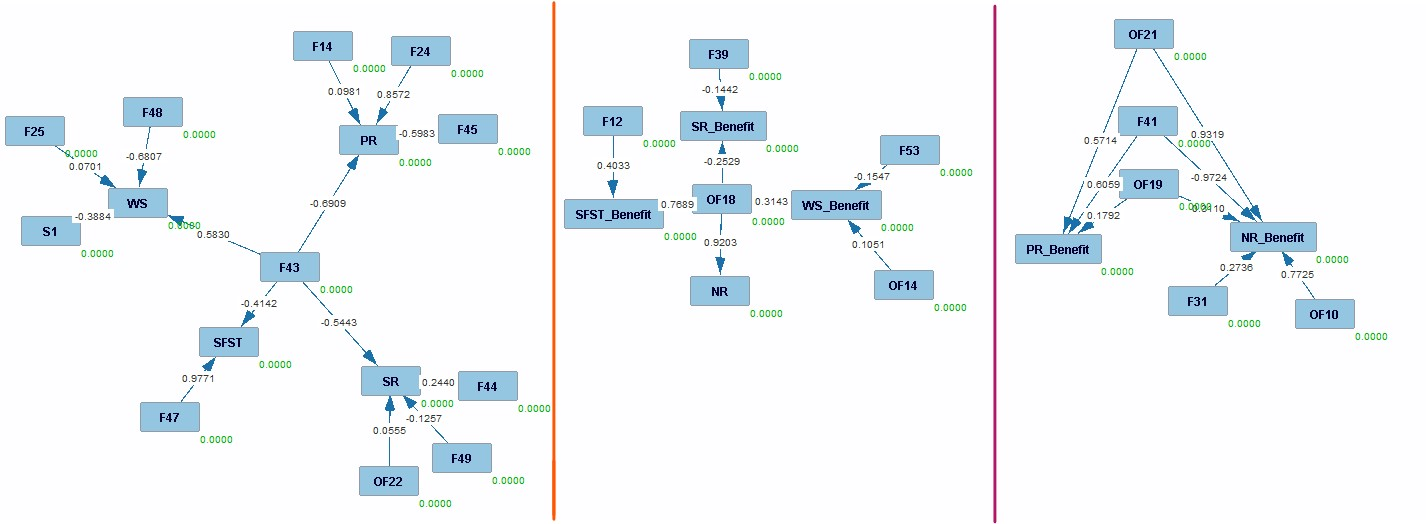
\includegraphics[width=0.95\linewidth]{tetrad/ex1.jpg}
    \caption{NR - Example of Tetrad Output}
    \label{fig:tetrad}
\end{figure}

After multiple iterations of Tetrad yielding no results, we turned our efforts towards \ac{ML}.
Further exploration with \ac{CI} or Tetrad specialists could be beneficial for this aspect of the project.




\section{Future Directions}
\subsection{Data}

This project presents several opportunities for future improvement, particularly in the area of data management and utilization. 
A more detailed analysis of the existing dataset could greatly enhance both our models and our understanding of the underlying processes.
By thoroughly analyzing the input variables and output possibilities, we can gain deeper insights into the behavior of certain results and model performance.

Expanding the dataset by incorporating new data or employing data augmentation techniques to increase the number of sites could significantly benefit our models.
Introducing data from different provinces or countries would enhance the generalizability and robustness of the models, making them more reliable across diverse regions.
Since visiting sites for data collection can be resource-intensive, leveraging calibration sites during training could provide a practical and efficient alternative.

Exploring different normalization techniques alongside model training could also yield promising results.
Currently, the normalization process is based on minimum and maximum values, which sometimes causes new sites to fall outside the expected bounds. Implementing alternative normalization methods, such as Z-score normalization or percentile-based scaling, could ensure that new sites remain within appropriate bounds, thereby improving model accuracy and applicability.

Incorporating additional features could further refine our models by reducing the number of input variables required.
Features such as provincial and federal classifications have already shown potential in improving the prediction of ecosystem function (\ac{EF}) scores and ratings.
Additionally, integrating historical data could enable long-term tracking of wetland performance, providing valuable insights into temporal changes and trends.

Future work could also explore the integration of remote sensing data to complement field data.
This could reduce the need for on-site visits and provide a more comprehensive view of wetland conditions over time.
Moreover, developing a dynamic dataset that updates in real-time as new data becomes available would allow for continuous model improvement and more accurate predictions.

\subsection{Machine Learning}

There are multiple avenues for advancing the machine learning algorithms used in this project, particularly in classification and regression tasks.
One promising direction is the implementation of more sophisticated neural network models.
Currently, we employ a simple neural network with a limited number of layers, which leaves considerable room for enhancement.
Incorporating deeper architectures, experimenting with different types of layers (such as convolutional, recurrent, or attention mechanisms) could be interesting.
Furthermore, exploring various methods of layer concatenation and architectural design could significantly boost model performance.

In future work, it would be beneficial to explore different ensemble learning techniques, such as a voting system.
Techniques such as bagging, boosting, or stacking could be investigated to determine their efficacy in predicting \ac{EF} scores.
Additionally, implementing transfer learning, where a pre-trained model on a large dataset is fine-tuned on our specific data, could accelerate the training process and improve model accuracy, especially since the available data is limited.

Hyperparameter optimization techniques, other than grid search, such as random search or Bayesian optimization, could be employed to fine-tune model parameters.
This could potentially lead to further improvements in performance. Furthermore, incorporating advanced algorithms like Gradient Boosting Machines (GBM) or Extreme Gradient Boosting (XGBoost) could be explored as alternatives or complements to neural networks.

\subsection{Causal Inference}

While much of our work has focused on machine learning, there are several potential improvements for causal inference (\ac{CI}) that could be explored. First, incorporating additional algorithms and expanding the dataset used in CausalML could improve the quality and reliability of our results.
A thorough, in-depth analysis of these results could further enhance our understanding and interpretation of the causal relationships at play.

For the Tetrad software, our initial attempts did not yield conclusive results.
Engaging with Tetrad experts to review our methodology and findings could be highly beneficial.
Expert consultation could help us validate our approach, refine our methods, and potentially unlock new insights that were previously inaccessible.

Future work could also involve integrating causal inference with machine learning models to create hybrid models that leverage the strengths of both approaches.
For example, causal inference could be used to identify the most influential features, which could then be used to inform feature selection in machine learning models.
Additionally, exploring other causal inference frameworks and tools, such as DoWhy or Pyro, could provide alternative perspectives and methodologies that may yield better results.

Moreover, developing a more comprehensive causal model that accounts for potential confounders and interactions between variables could enhance the robustness of our findings.
Finally, validating the causal relationships identified through field experiments or observational studies could provide empirical support for the model predictions and strengthen the overall conclusions of the study.


\section{Conclusion}
This report presented a detailed analysis of various ecosystem functions (\acp{EF}) using a combination of classification and regression models, integrated with causal inference techniques and ensemble learning methods.
Our objective was to evaluate the effectiveness of different feature sets in predicting \ac{EF} scores, to assess the potential of specific features versus all available features and to explore the causal relationships between features and their effects on the \acp{EF} using advanced tools like CausalML and Tetrad.
Our study began by outlining the importance of ecosystem functions, which are critical to understanding the health and sustainability of natural environments.
The accurate prediction and assessment of these functions are vital for environmental management, conservation efforts and policy-making.
We employed various machine learning techniques to predict the scores of different \acp{EF}, including Phosphorus Retention (\ac{PR}), Nitrate Removal \& Retention (\ac{NR}), Sediment Retention \& Stabilization (\ac{SR}), Water Storage \& Delay (\ac{WS}) and Stream Flow Support (\ac{SFST}).
These \acp{EF} were analyzed not only in terms of their direct functions but also their benefits (\ac{BS}) to human populations.

\subsection{Classification Analysis}
We began with the classification of \acp{EF}, where we compared the performance of models trained on all features versus those trained on a reduced set of specific features.
The classification models aimed to categorize sites based on their \ac{EF} scores into predefined classes, enabling us to determine how well the models could generalize across different datasets.
Our results demonstrated that while classification using all features generally outperformed the models trained on specific features, certain \acp{EF}, such as \ac{PR} and \ac{WS}, showed robust performance even with a reduced feature set.
This indicates that for these functions, key features carry significant predictive power, allowing for more efficient modeling with fewer data points.
However, for other \acp{EF} like \ac{SR} and \ac{SFST}, the reduction in features led to a noticeable drop in classification accuracy, highlighting the importance of maintaining a comprehensive set of features for complex functions.
The results also revealed that ensemble learning techniques did not universally enhance model performance, with some \acp{EF} benefiting from ensemble methods while others experienced reduced accuracy.

\subsection{Regression Analysis}
Following the classification analysis, we delved into regression models to predict the exact \ac{EF} scores.
Regression provided a more nuanced understanding of the relationships between features and \ac{EF} outcomes, allowing us to generate continuous predictions rather than categorical classifications.
The regression models, similar to the classification models, were tested on both the full set of features and the reduced specific features dataset.
Our findings indicated that regression models generally performed better when utilizing all features, particularly for complex \acp{EF} such as \ac{SR} and \ac{SFST}, where the comprehensive dataset allowed for more accurate predictions.
Interestingly, for certain \acp{EF} like \ac{PR} and \ac{NR}, the models trained on specific features performed comparably to those trained on all features, suggesting that the most influential features for these functions were included in the reduced dataset.
Additionally, our analysis showed that regression models often outperformed classification models in terms of predictive accuracy, making them more suitable for detailed \ac{EF} assessments.


\subsection{Phosphorus Retention (\ac{PR})}
Phosphorus Retention is a crucial \ac{EF} as it plays a significant role in maintaining the ecological balance by preventing excess phosphorus from entering water bodies, which can lead to eutrophication.
Our analysis showed that \ac{PR} performed well with both classification and regression models, especially when using specific features.
Key features such as F43 (Channel Connection and Outflow Duration), F44 (Outflow Confinement) and F45 (Through Flow Resistance) consistently appeared as important predictors, demonstrating their significance in phosphorus retention.
These features, which are related to the wetland's hydrological connectivity and water retention capacity, directly influence the ability of a wetland to retain phosphorus over time.
Interestingly, when focusing on \ac{PR} Benefit, which evaluates the human benefits of phosphorus retention, additional features such as OF19 (Water Quality Downstream) and OF22 (Wetland Size Relative to Catchment) became crucial.
This distinction between function and benefit underscores the complexity of environmental modeling, where the ecological role of a feature might differ from its perceived human value.
Regression models, particularly those using specific features, provided high accuracy, suggesting that \ac{PR} can be effectively predicted with a carefully selected subset of features, enabling more efficient environmental assessments.

\subsection{Nitrate Removal \& Retention (\ac{NR})}
Nitrate Removal \& Retention is another vital \ac{EF}, particularly in its role in reducing nitrogen pollution through the process of denitrification.
Our study revealed that \ac{NR} is more challenging to predict than \ac{PR}, requiring a broader set of features to achieve high accuracy.
However, similar to \ac{PR}, features related to water retention and connectivity, such as F43, F44 and F45, were consistently important across models.
The regression models showed that \ac{NR} could be predicted with high accuracy when using these key features, especially with specific feature sets.
For \ac{NR} Benefit, which considers the impact on human populations, the most significant features included those related to water quality and proximity to human activities, such as OF9 (Distance to Domestic Wells) and OF10 (Nearest Population Center).
This indicates that human-related factors play a significant role in determining the benefit of nitrate retention, highlighting the need for models that integrate both environmental and human dimensions.
The successful prediction of \ac{NR} Benefit using regression models with a reduced feature set demonstrates the potential for efficient monitoring and management practices.

\subsection{Sediment Retention \& Stabilization (\ac{SR})}
Sediment Retention \& Stabilization is crucial for preventing soil erosion, maintaining water quality and supporting aquatic habitats.
Our analysis found that \ac{SR} was particularly challenging to predict, especially with classification models using specific features, which often resulted in lower accuracy compared to other \acp{EF}.
Key features such as F28 (Annual Water Fluctuation), F31 (Percentage of Ponded Water) and F44 were vital in predicting \ac{SR}, indicating that the ability of wetlands to stabilize sediments is closely tied to their hydrological characteristics.
The regression models provided better predictions for \ac{SR}, especially when using all available features, which suggests that sediment retention is a complex process influenced by multiple factors.
For \ac{SR} Benefit, features related to water quality and hydrological connectivity, such as OF19 and F41 (Tributary Channels), were essential, reflecting the importance of both environmental and human-related factors in determining the benefits of sediment retention.
The mixed results for \ac{SR} highlight the complexity of this function and suggest that future models may need to incorporate more comprehensive datasets or advanced modeling techniques to improve accuracy.

\subsection{Water Storage \& Delay (\ac{WS})}
Water Storage \& Delay is a fundamental \ac{EF} that helps to mitigate flooding, sustain base flows during dry periods and support other \acp{EF} like sediment retention and nutrient removal.
Our findings indicated that \ac{WS} was one of the most predictable \acp{EF}, with regression models achieving high accuracy, particularly when using specific features.
Key features for \ac{WS} included F22 (Percentage of Area Seasonally Flooded), F28 and F43, all of which are directly related to the wetland’s capacity to store and manage water.
These results suggest that \ac{WS} is strongly influenced by the physical and hydrological properties of the wetland, making it a relatively straightforward function to model.
Interestingly, the \ac{WS} Benefit could be accurately predicted using only a few \ac{OF} features, such as OF17 (Flood Damage from Non-Tidal Waters) and OF23 (Unvegetated Surface in the Contributing Area).
This suggests that for \ac{WS}, it may be possible to conduct effective assessments with minimal field data, relying instead on observable or remotely sensed information.
The ability to predict \ac{WS} Benefit with high accuracy using limited features highlights the potential for simplifying environmental assessments, particularly in large-scale or remote regions where field data collection is challenging.

\subsection{Stream Flow Support (\ac{SFST})}
Stream Flow Support is essential for maintaining base flows in streams, especially during dry periods and for supporting aquatic life.
Our analysis showed that \ac{SFST} was one of the most challenging \acp{EF} to predict, particularly its benefit to human populations.
The \ac{SFST} function itself was best predicted using features like F1 (Overall Vegetation, Water and Soil) and F43, which are indicative of the wetland’s ability to contribute water to streams.
However, the \ac{SFST} Benefit was difficult to model accurately, especially when using specific features, with significant drops in accuracy observed.
This suggests that the factors influencing \ac{SFST} Benefit are more complex and perhaps less directly observable than those influencing the \ac{SFST} function.
The disparity in model performance between the \ac{SFST} function and its benefit highlights the need for further research into the drivers of stream flow support, particularly in understanding how human activities and land-use changes affect this critical function.

\subsection{Causal Inference with CausalML}
To further enhance our understanding of feature importance and the underlying relationships between features and \acp{EF}, we employed CausalML, a Python library that integrates causal inference with machine learning.
This approach allowed us to move beyond correlation and explore causality, identifying which features have a direct impact on \ac{EF} outcomes.
Through CausalML, we were able to rank the features based on their importance, using both average importance scores and a custom point system.
The results reinforced our earlier findings, with features such as F43 consistently emerging as crucial across multiple \acp{EF}.
The causal analysis provided valuable insights into the mechanics of each \ac{EF}, highlighting the features that drive the most significant changes in \ac{EF} scores.
This understanding is crucial for environmental management, as it allows for more targeted interventions and resource allocation.

\subsection{Challenges with Tetrad}
In an attempt to explore the causal relationships further, we utilized Tetrad, a software tool designed for discovering causal relationships between variables.
Despite multiple iterations and adjustments to the models, Tetrad did not yield any significant results that could be integrated into our analysis.
The lack of fitting models led us to reconsider our approach and focus more on the insights provided by CausalML.
Future work in this area could benefit from collaboration with specialists in causal inference to fully leverage Tetrad's capabilities.

\subsection{Overall Conclusion}
In conclusion, this report has provided a comprehensive analysis of ecosystem functions using advanced machine learning techniques and causal inference tools.
Our findings underscore the importance of selecting the right set of features for accurate predictions, particularly when dealing with complex environmental functions like \ac{SR} and \ac{SFST}.
While feature reduction can streamline models and reduce data requirements, it is not without risks, as the exclusion of important variables can significantly impact model performance.
The integration of causal inference techniques like CausalML offers a promising avenue for better understanding the dynamics at play within these ecosystems, providing a more informed basis for environmental decision-making.
Moving forward, future research should continue to explore the balance between model complexity and accuracy, the potential of ensemble methods and the application of causal inference in environmental science.
By doing so, we can improve our ability to model, understand and ultimately protect the vital ecosystem functions that sustain our planet.










\bibliography{references.bib}
\bibliographystyle{IEEEtran}

\clearpage
\section{Annexes}
\subsection{Datasets}
\begin{table}[h]
    \centering
    \begin{tabular}{|m{3cm}|c|m{11cm}|}
        \hline
        \textbf{Feature Name} & \textbf{Type} & \textbf{Description} \\
        \hline
        Provincial Class & Class (6) & This classification divides wetlands into six distinct types based on their ecological characteristics. It aids in the management and conservation of wetland resources. \\
        \hline
        Provincial Class & Class (10) & This extended classification categorizes wetlands into ten types, providing a more detailed understanding of wetland diversity for conservation strategies. \\
        \hline
        Water Regime & Class (4) & This indicator classifies water regimes into four types, describing the hydrological conditions of a wetland. It is essential for wetland management. \\
        \hline
        Vegetation Type & Class (7) & This classification identifies seven types of specific vegetation present in wetlands. It helps in assessing the ecological status of wetland areas. \\
        \hline
        Veg. Cover & Class (5) & This classification indicates the percentage cover of specific vegetation types, divided into five classes. It provides insights into vegetation distribution. \\
        \hline
        Woody Canopy & Class (4) & This classification describes the percentage cover of high woody canopy (over 5 meters), divided into four classes. It is useful for understanding forest structure in wetlands. \\
        \hline
        \% Moss Cover & Class (5) & This classification specifies the percentage cover of moss in wetlands, divided into five classes. It is important for ecological assessments. \\
        \hline
        Phragmites  & Class (3) & This feature indicates the presence of Phragmites (an invasive plant species) in a wetland, classified as yes or no. It is crucial for invasive species management. \\
        \hline
        Soil Type & Class (3) & This classification identifies the soil types in wetlands, divided into three classes. It helps in understanding soil characteristics and their impact on wetland ecology. \\
        \hline
        Surface Water & Class (7) & This classification indicates the percentage of surface water present in a wetland, divided into seven classes. It is important for hydrological studies. \\
        \hline
        Depth Sat. & Class (4) & This feature measures the depth of water saturation in soil, divided into four classes. It helps in understanding soil moisture conditions. \\
        \hline
        Depth Moss & Float & This feature measures the average depth of living moss in centimeters. It provides insights into the health and growth of moss in wetlands. \\
        \hline
        Organic Depth & Float & This feature measures the average depth of organic material in soil in centimeters. It is crucial for understanding soil composition and fertility. \\
        \hline
        Hydrogeomorphic & Class (11) & This classification divides wetlands into eleven hydrogeomorphic classes, based on their geomorphology and hydrology. It is essential for wetland characterization and management. \\
        \hline
    \end{tabular}
    \caption{Feature Descriptions for Various Wetland Attributes}
    \label{tab:data_xtra_features}
\end{table}


\subsection{Features}


\clearpage
\subsection{Machine Learning Algorithms}\label{sec:algorithms}
\begin{longtable}{|>{\raggedright}p{2cm}|>{\raggedright}p{3cm}|>{\raggedright\arraybackslash}p{8cm}|}
\hline
\textbf{Algorithm} & \textbf{Type} & \textbf{Parameters} \\
\hline
Ridge & Class./Reg. & 
\begin{itemize}
    \item \texttt{alpha}: [0.1, 0.5, 1.0]
    \item \texttt{solver}: ['auto', 'svd', 'cholesky', 'lsqr', 'sparse\_cg', 'sag', 'saga', 'lbfgs']
\end{itemize} \\
\hline
Decision Tree & Class./Reg. & 
\begin{itemize}
    \item \texttt{criterion}: ['gini', 'entropy', 'log\_loss'] (Class.), ['squared\_error', 'friedman\_mse', 'absolute\_error', 'poisson'] (Reg.)
    \item \texttt{splitter}: ['best', 'random']
    \item \texttt{min\_samples\_split}: [2, 3, 4, 5]
    \item \texttt{max\_features}: [None, 'sqrt', 'log2']
\end{itemize} \\
\hline
Random Forest & Class./Reg. & 
\begin{itemize}
    \item \texttt{n\_estimators}: [50, 100, 200]
    \item \texttt{criterion}: ['gini', 'entropy', 'log\_loss'] (Class.), ['squared\_error', 'friedman\_mse', 'absolute\_error', 'poisson'] (Reg.)
    \item \texttt{min\_samples\_split}: [2, 5]
    \item \texttt{max\_features}: ['sqrt', 'log2']
\end{itemize} \\
\hline
Gradient Boosting & Class./Reg. & 
\begin{itemize}
    \item \texttt{loss}: ['log\_loss', 'deviance', 'exponential'] (Class.), ['squared\_error', 'absolute\_error', 'huber', 'quantile'] (Reg.)
    \item \texttt{learning\_rate}: [0.001, 0.01, 0.1]
    \item \texttt{n\_estimators}: [50, 100, 200]
    \item \texttt{warm\_start}: [True, False]
\end{itemize} \\
\hline
AdaBoost & Class./Reg. & 
\begin{itemize}
    \item \texttt{n\_estimators}: [50, 100, 200]
    \item \texttt{learning\_rate}: [0.001, 0.01, 0.1, 1.0]
    \item \texttt{algorithm}: ['SAMME', 'SAMME.R'] (Class.), \texttt{loss}: ['linear', 'square', 'exponential'] (Reg.)
\end{itemize} \\
\hline
K-Neighbors & Class./Reg. & 
\begin{itemize}
    \item \texttt{n\_neighbors}: [5, 10, 15, 20]
    \item \texttt{weights}: ['uniform', 'distance']
    \item \texttt{algorithm}: ['auto', 'ball\_tree', 'kd\_tree', 'brute']
    \item \texttt{leaf\_size}: [30, 50, 70]
    \item \texttt{metric}: ['euclidean', 'manhattan', 'minkowski']
\end{itemize} \\
\hline
MLP (Neural Network) & Class./Reg. & 
\begin{itemize}
    \item \texttt{hidden\_layer\_sizes}: [(50, 50, 50), (100, 100, 100), (100, 100, 100, 100)]
    \item \texttt{activation}: ['identity', 'logistic', 'tanh', 'relu']
    \item \texttt{solver}: ['lbfgs', 'sgd', 'adam']
    \item \texttt{learning\_rate}: ['constant', 'invscaling', 'adaptive']
\end{itemize} \\
\hline
Logistic Regression & Classifier & 
\begin{itemize}
    \item \texttt{penalty}: ['l1', 'l2', 'elasticnet', 'none']
    \item \texttt{C}: [0.1, 0.5, 1.0, 5.0, 10.0]
    \item \texttt{solver}: ['newton-cg', 'lbfgs', 'liblinear', 'sag', 'saga']
    \item \texttt{max\_iter}: [100, 200, 300]
\end{itemize} \\
\hline
SGD & Class./Reg. & 
\begin{itemize}
    \item \texttt{loss}: ['hinge', 'log', 'modified\_huber', 'squared\_hinge', 'perceptron'] (Class.), ['squared\_error', 'huber', 'epsilon\_insensitive', 'squared\_epsilon\_insensitive'] (Reg.)
    \item \texttt{penalty}: ['l2', 'l1', 'elasticnet']
    \item \texttt{learning\_rate}: ['constant', 'optimal', 'invscaling', 'adaptive']
    \item \texttt{warm\_start}: [True, False]
\end{itemize} \\
\hline
Support Vector Machines (SVM) & Class./Reg. & 
\begin{itemize}
    \item \texttt{C}: [0.1, 1.0, 10.0]
    \item \texttt{kernel}: ['linear', 'poly', 'rbf', 'sigmoid']
    \item \texttt{degree}: [1, 3, 5]
    \item \texttt{gamma}: ['scale', 'auto']
\end{itemize} \\
\hline
Gaussian Naive Bayes & Classifier & 
\begin{itemize}
    \item \texttt{var\_smoothing}: [1e-9, 1e-8, 1e-7]
\end{itemize} \\
\hline
Linear Discriminant Analysis & Classifier & 
\begin{itemize}
    \item \texttt{solver}: ['svd', 'lsqr', 'eigen']
    \item \texttt{shrinkage}: [None, 'auto', 0.1, 0.5, 1.0]
\end{itemize} \\
\hline
ElasticNet & Regressor & 
\begin{itemize}
    \item \texttt{l1\_ratio}: [0.25, 0.5, 0.75]
    \item \texttt{fit\_intercept}: [True, False]
    \item \texttt{precompute}: [True, False]
    \item \texttt{copy\_X}: [True, False]
    \item \texttt{warm\_start}: [True, False]
    \item \texttt{positive}: [True, False]
    \item \texttt{selection}: ['cyclic', 'random']
\end{itemize} \\
\hline
Bayesian Ridge & Regressor & 
\begin{itemize}
    \item \texttt{alpha\_1}: [1e-7, 1e-6, 1e-5]
    \item \texttt{alpha\_2}: [1e-7, 1e-6, 1e-5]
    \item \texttt{lambda\_1}: [1e-7, 1e-6, 1e-5]
    \item \texttt{lambda\_2}: [1e-7, 1e-6, 1e-5]
\end{itemize} \\
\hline
Kernel Ridge & Regressor & 
\begin{itemize}
    \item \texttt{alpha}: [0.00001, 0.0001, 0.001, 0.01]
    \item \texttt{kernel}: ['linear', 'poly', 'rbf', 'sigmoid', 'precomputed']
    \item \texttt{degree}: [1, 2, 3, 5, 10]
    \item \texttt{coef0}: [0.0, 0.5, 1.0]
\end{itemize} \\
\hline
Linear Regression & Regressor & 
\begin{itemize}
    \item \texttt{fit\_intercept}: [True, False]
    \item \texttt{copy\_X}: [True, False]
    \item \texttt{positive}: [True, False]
\end{itemize} \\
\hline
RANSAC Regressor & Regressor & 
\begin{itemize}
    \item \texttt{min\_samples}: [None, 1, 2, 5, 10]
    \item \texttt{max\_trials}: [1, 10, 50, 100, 150]
    \item \texttt{loss}: ['absolute\_error', 'squared\_error']
\end{itemize} \\
\hline
Theil-Sen Regressor & Regressor & 
\begin{itemize}
    \item \texttt{max\_subpopulation}: [1, 10, 100, 500]
    \item \texttt{n\_subsamples}: [None, 1, 5, 10, 25]
\end{itemize} \\
\hline

\caption{Machine Learning Algorithms}
\label{tab:all_algorithms}
\end{longtable}

\subsection{Classification}\label{sec:class_annex}
\subsubsection{All Features}
\begin{figure}[H]
    \centering
    \begin{minipage}[b]{0.45\textwidth}
            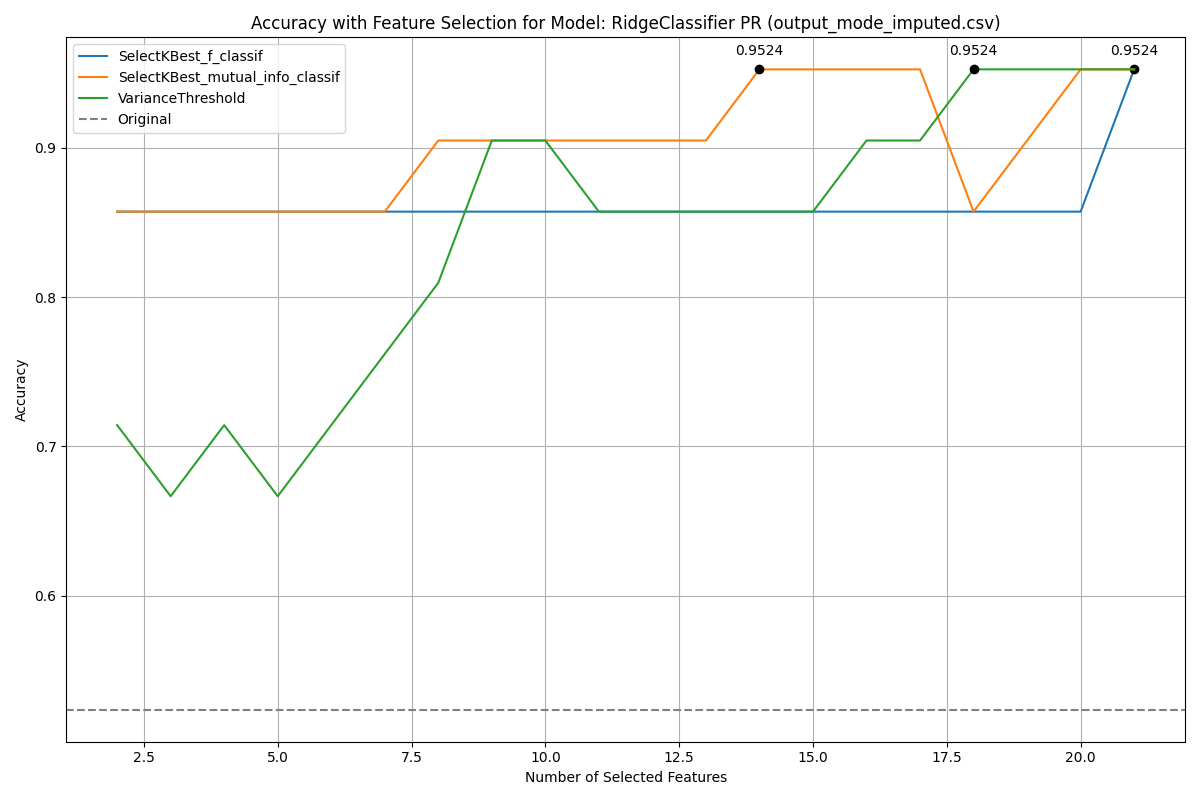
\includegraphics[width=\textwidth]{class_specific_section/images_class_ensemble_reduction/feature_selection_accuracy_plot_output_mode_imputedcsv_RidgeClassifier_PR.png}
        \caption{PR}
        \label{fig_class_spec:pr_featred_graph}
    \end{minipage}
    \hfill
    \begin{minipage}[b]{0.45\textwidth}
        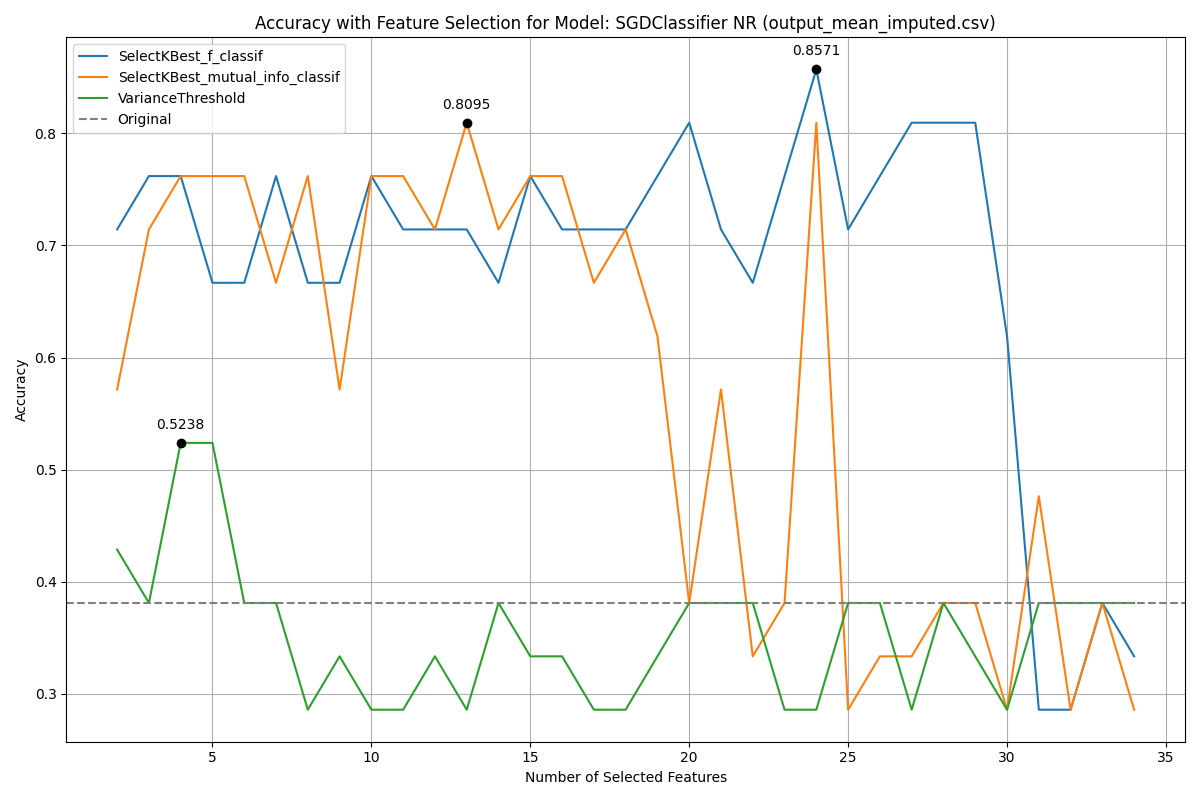
\includegraphics[width=\textwidth]{class_specific_section/images_class_ensemble_reduction/feature_selection_accuracy_plot_output_mean_imputedcsv_SGDClassifier_NR.png}
        \caption{NR}
        \label{fig_class_spec:nr_featred_graph}
    \end{minipage}
\end{figure}

\begin{figure}[H]
    \centering
    \begin{minipage}[b]{0.45\textwidth}
        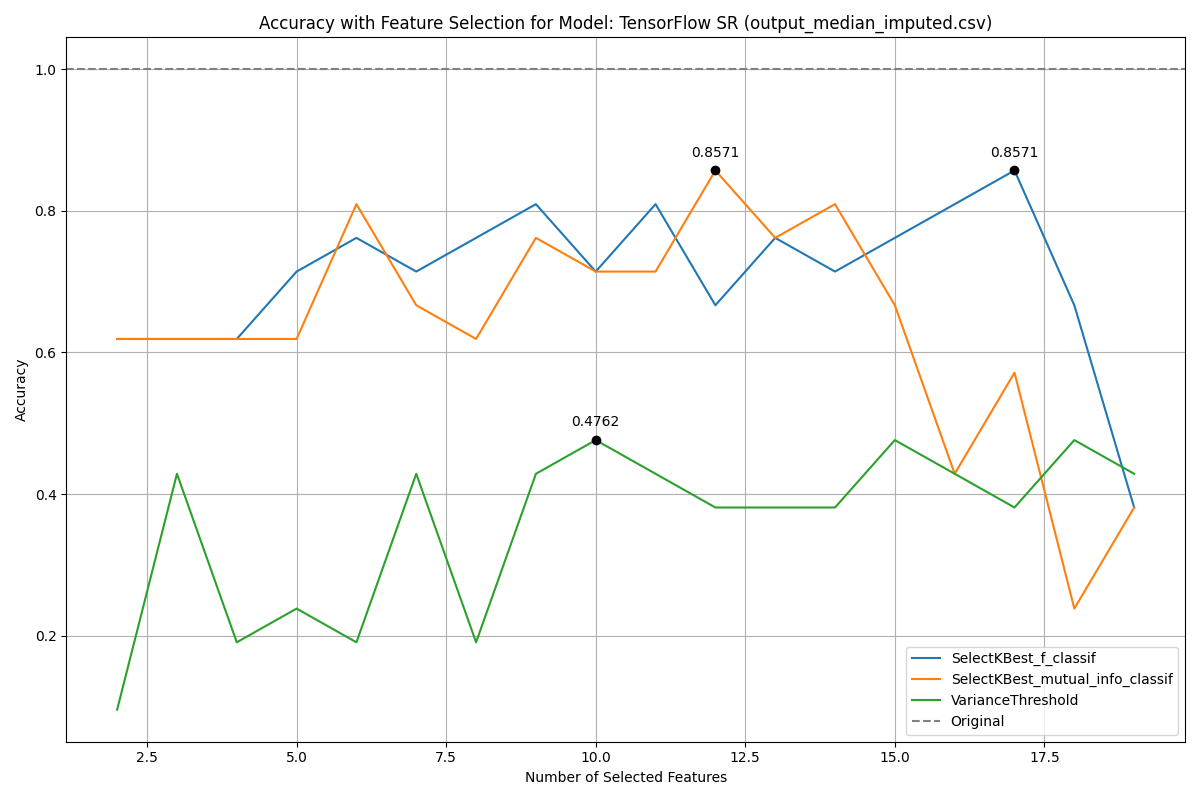
\includegraphics[width=\textwidth]{class_specific_section/images_class_ensemble_reduction/feature_selection_accuracy_plot_output_median_imputedcsv_TensorFlow_SR.png}
        \caption{SR}
        \label{fig_class_spec:sr_featred_graph}
    \end{minipage}
    \hfill
    \begin{minipage}[b]{0.45\textwidth}
        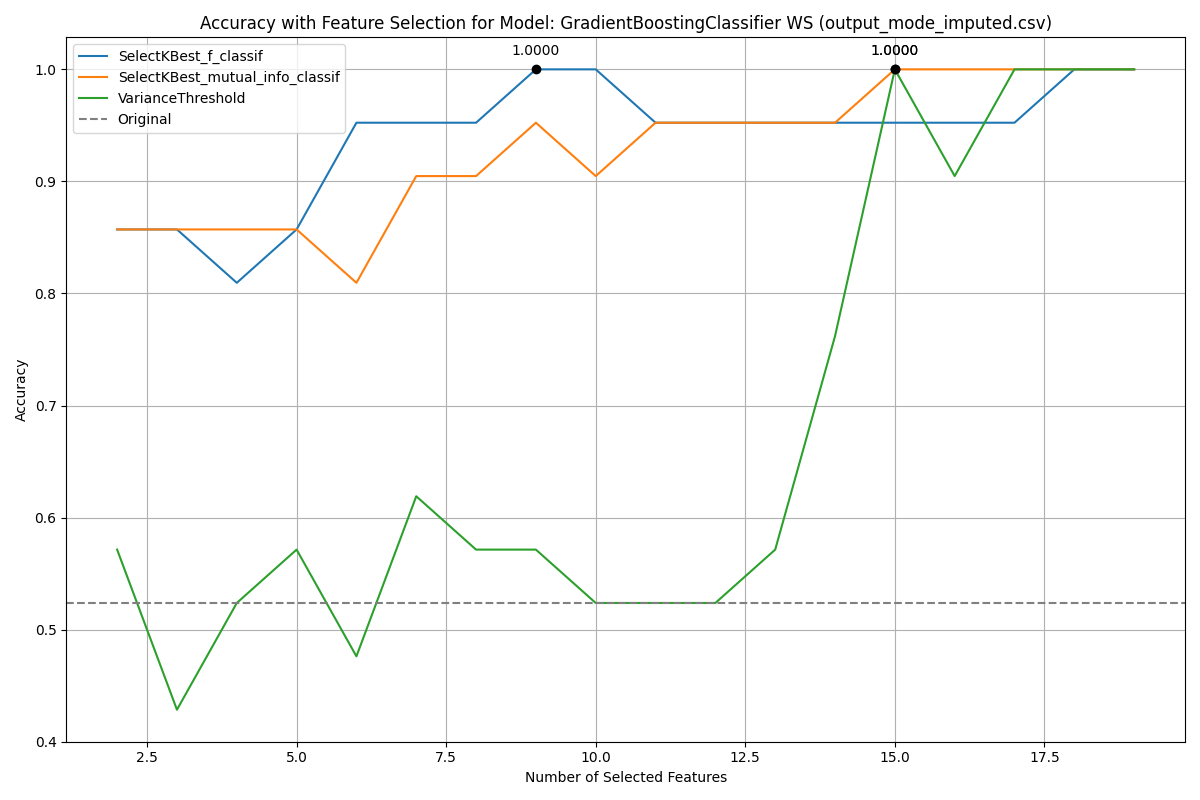
\includegraphics[width=\textwidth]{class_specific_section/images_class_ensemble_reduction/feature_selection_accuracy_plot_output_mode_imputedcsv_GradientBoostingClassifier_WS.png}
        \caption{WS}
        \label{fig_class_spec:ws_featred_graph}
    \end{minipage}
\end{figure}

\begin{figure}[H]
    \centering
    \begin{minipage}[b]{0.45\textwidth}
        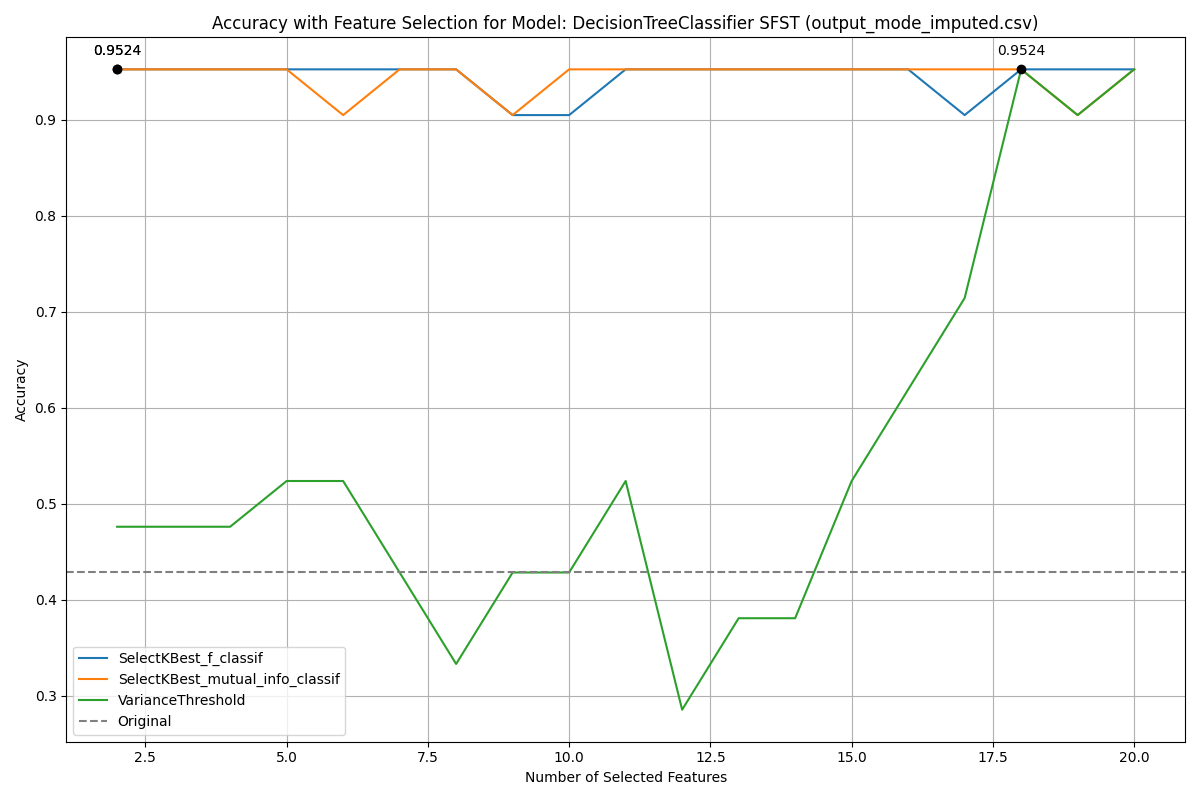
\includegraphics[width=\textwidth]{class_specific_section/images_class_ensemble_reduction/feature_selection_accuracy_plot_output_mode_imputedcsv_DecisionTreeClassifier_SFST.png}
        \caption{SFST}
        \label{fig_class_spec:sfst_featred_graph}
    \end{minipage}
    \hfill
    \begin{minipage}[b]{0.45\textwidth}
        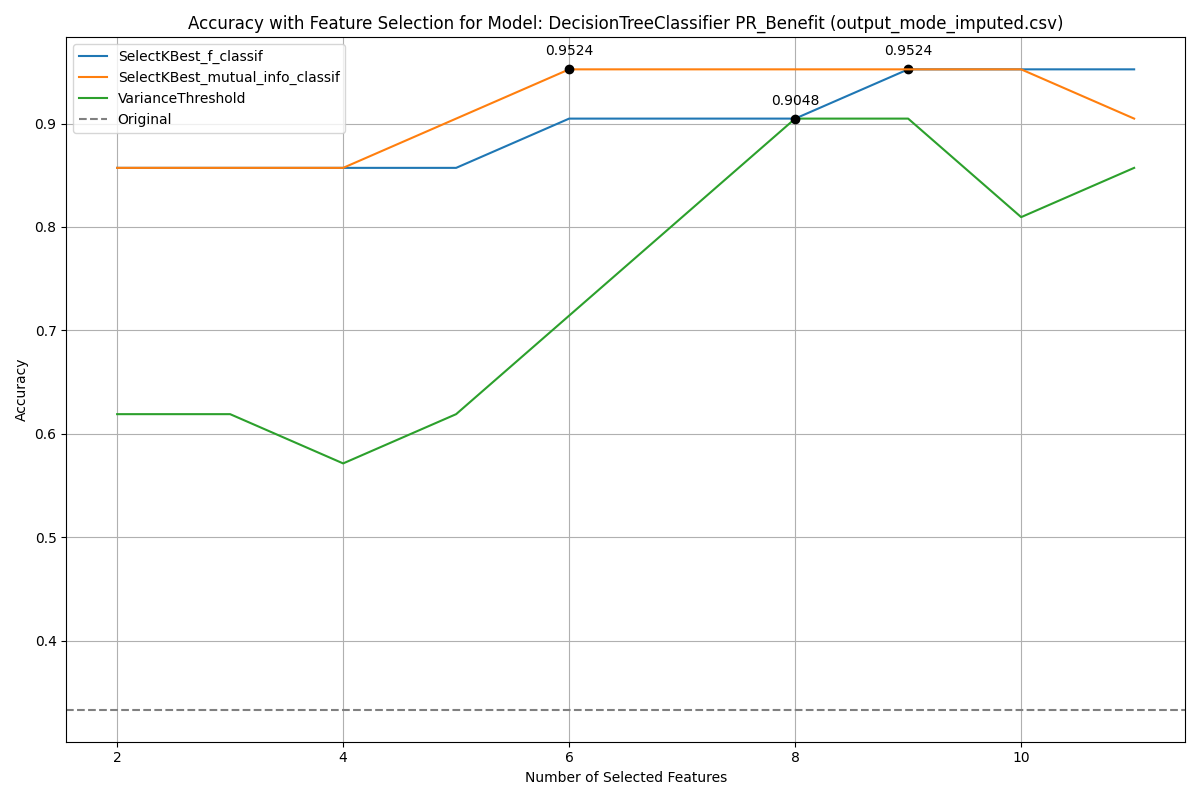
\includegraphics[width=\textwidth]{class_specific_section/images_class_ensemble_reduction/feature_selection_accuracy_plot_output_mode_imputedcsv_DecisionTreeClassifier_PR_Benefit.png}
        \caption{PR Benefit}
        \label{fig_class_spec:pr_ben_featred_graph}
    \end{minipage}
\end{figure}

\begin{figure}[H]
    \centering
    \begin{minipage}[b]{0.45\textwidth}
        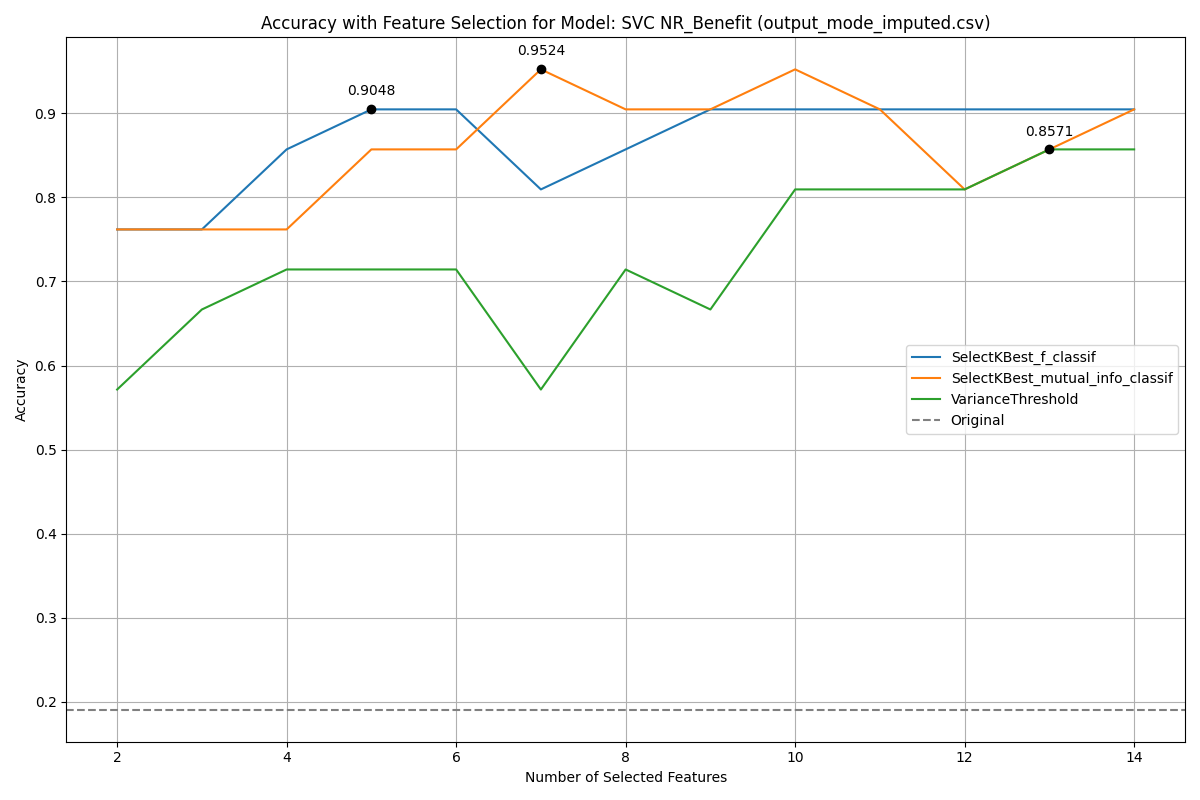
\includegraphics[width=\textwidth]{class_specific_section/images_class_ensemble_reduction/feature_selection_accuracy_plot_output_mode_imputedcsv_SVC_NR_Benefit.png}
        \caption{NR Benefit}
        \label{fig_class_spec:nr_ben_featred_graph}
    \end{minipage}
    \hfill
    \begin{minipage}[b]{0.45\textwidth}
        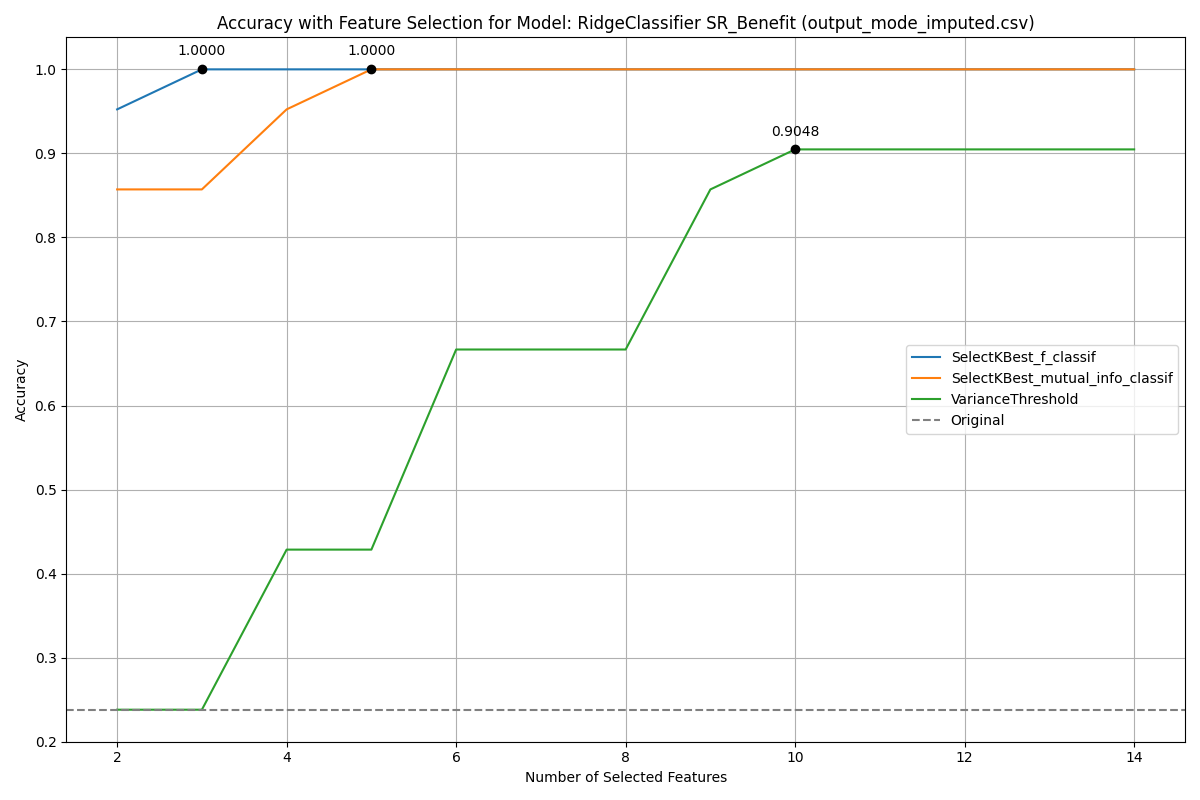
\includegraphics[width=\textwidth]{class_specific_section/images_class_ensemble_reduction/feature_selection_accuracy_plot_output_mode_imputedcsv_RidgeClassifier_SR_Benefit.png}
        \caption{SR Benefit}
        \label{fig_class_spec:sr_ben_featred_graph}
    \end{minipage}
\end{figure}

\begin{figure}[H]
    \centering
    \begin{minipage}[b]{0.45\textwidth}
        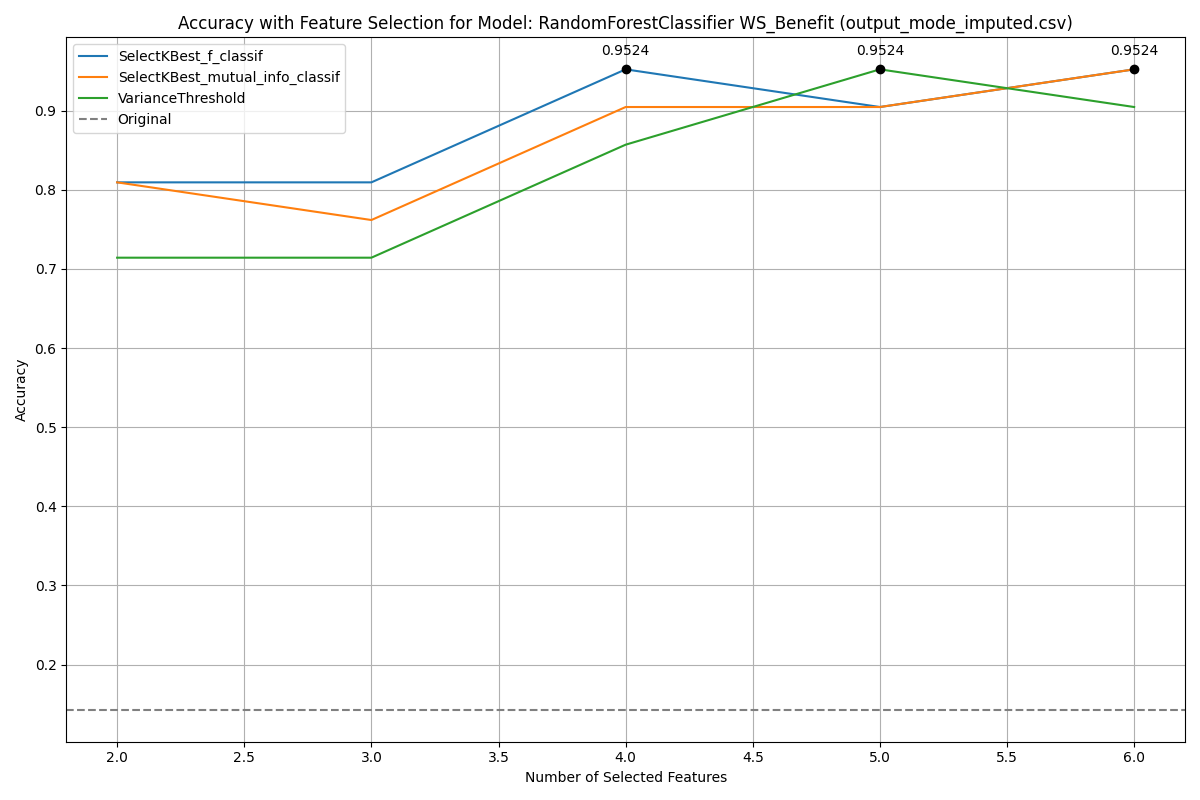
\includegraphics[width=\textwidth]{class_specific_section/images_class_ensemble_reduction/feature_selection_accuracy_plot_output_mode_imputedcsv_RandomForestClassifier_WS_Benefit.png}
        \caption{WS Benefit}
        \label{fig_class_spec:ws_ben_featred_graph}
    \end{minipage}
    \hfill
    \begin{minipage}[b]{0.45\textwidth}
        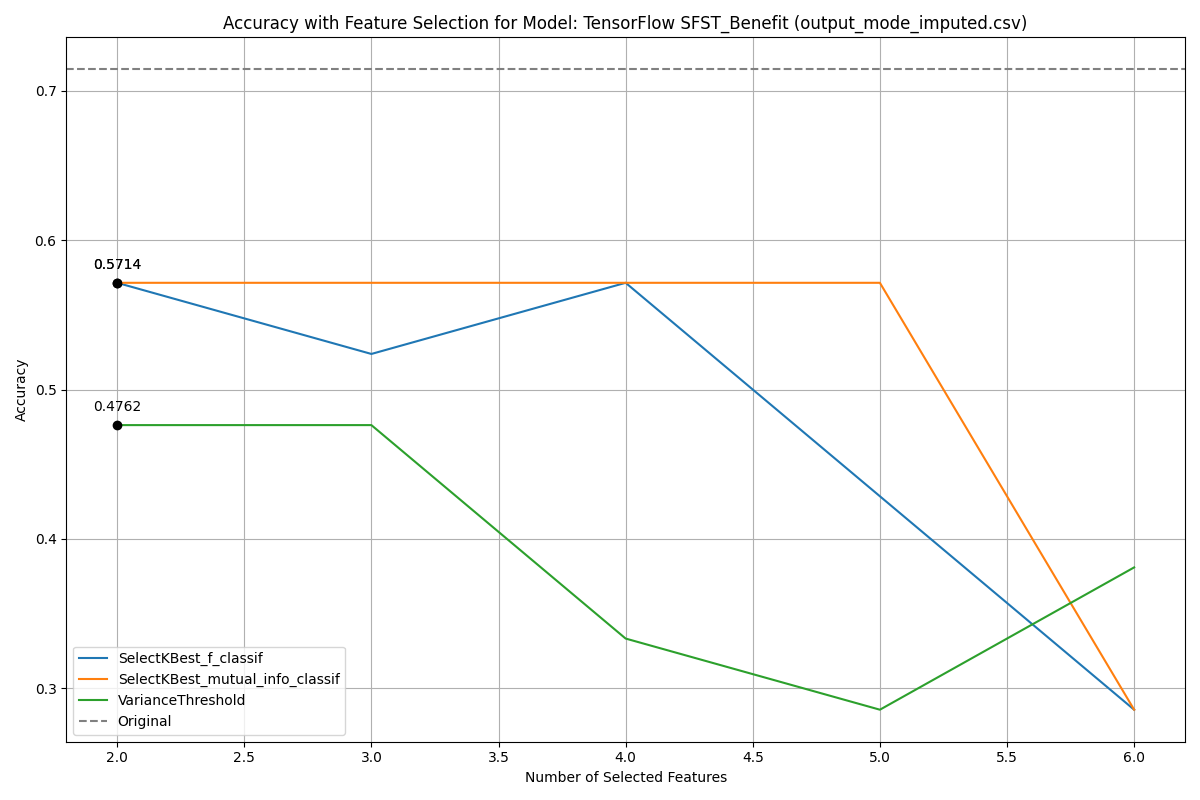
\includegraphics[width=\textwidth]{class_specific_section/images_class_ensemble_reduction/feature_selection_accuracy_plot_output_mode_imputedcsv_TensorFlow_SFST_Benefit.png}
        \caption{SFST Benefit}
        \label{fig_class_spec:sfst_ben_featred_graph}
    \end{minipage}
\end{figure}


\subsubsection{Specific Features}
\begin{figure}[H]
    \centering
    \begin{minipage}[b]{0.45\textwidth}
            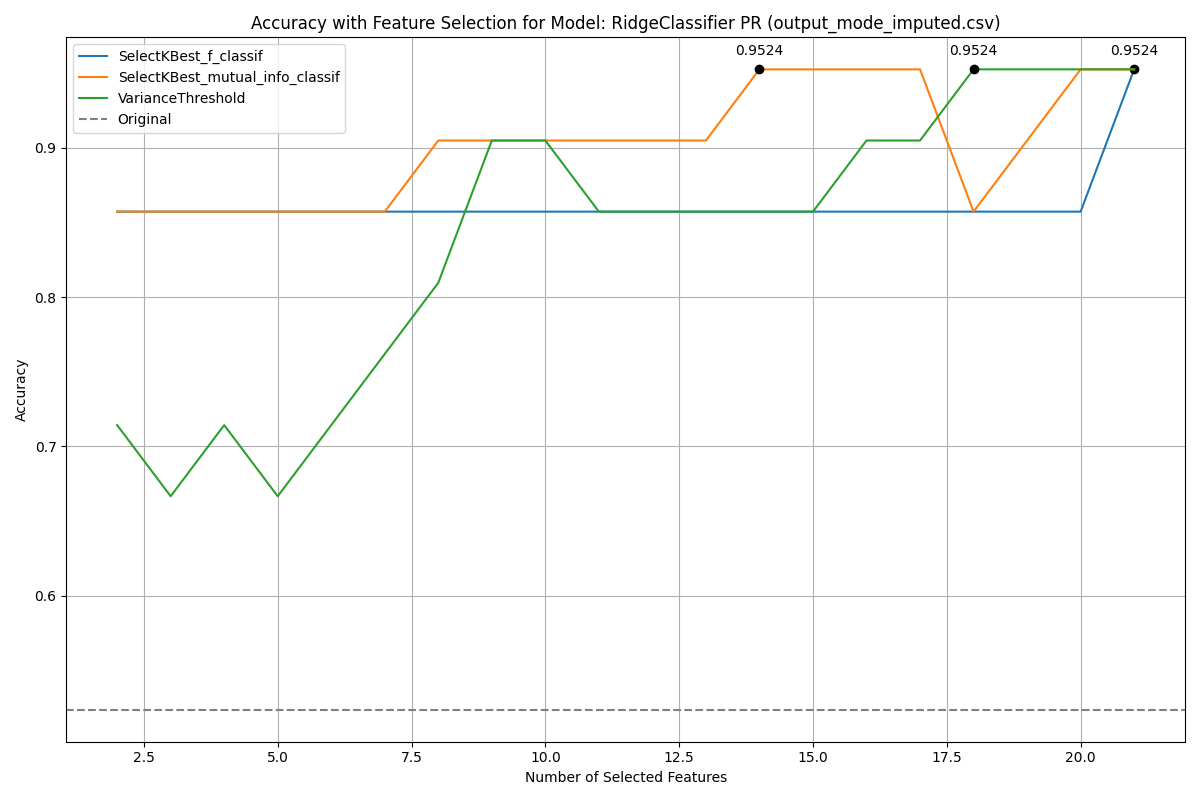
\includegraphics[width=\textwidth]{class_specific_section/images_class_ensemble_reduction/feature_selection_accuracy_plot_output_mode_imputedcsv_RidgeClassifier_PR.png}
        \caption{PR}
        \label{fig_class_spec:pr_featred_graph}
    \end{minipage}
    \hfill
    \begin{minipage}[b]{0.45\textwidth}
        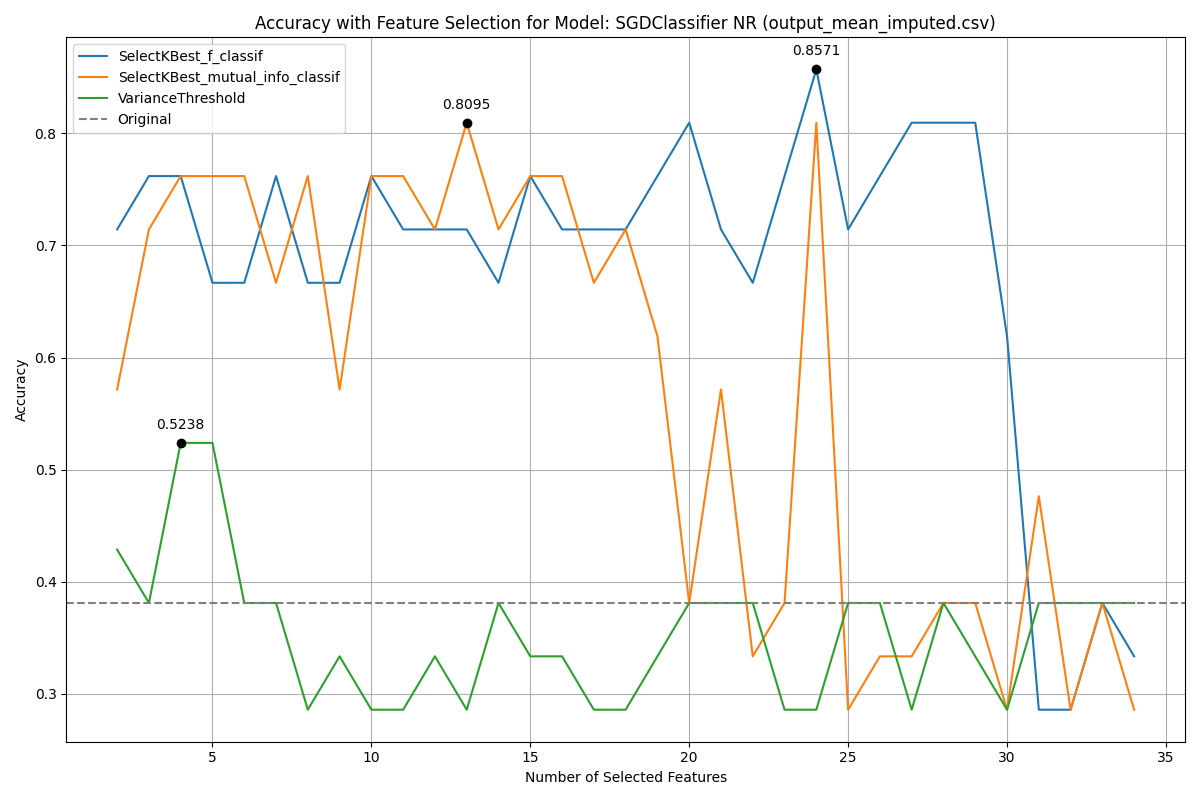
\includegraphics[width=\textwidth]{class_specific_section/images_class_ensemble_reduction/feature_selection_accuracy_plot_output_mean_imputedcsv_SGDClassifier_NR.png}
        \caption{NR}
        \label{fig_class_spec:nr_featred_graph}
    \end{minipage}
\end{figure}

\begin{figure}[H]
    \centering
    \begin{minipage}[b]{0.45\textwidth}
        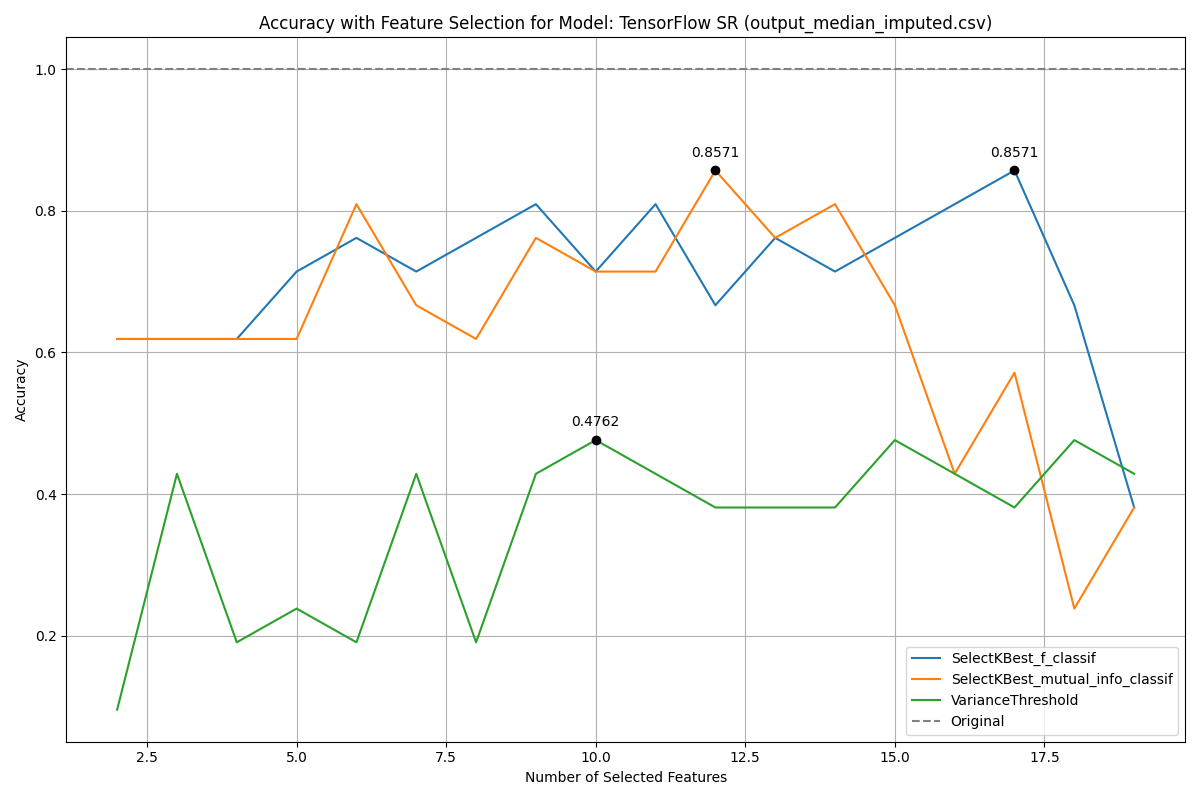
\includegraphics[width=\textwidth]{class_specific_section/images_class_ensemble_reduction/feature_selection_accuracy_plot_output_median_imputedcsv_TensorFlow_SR.png}
        \caption{SR}
        \label{fig_class_spec:sr_featred_graph}
    \end{minipage}
    \hfill
    \begin{minipage}[b]{0.45\textwidth}
        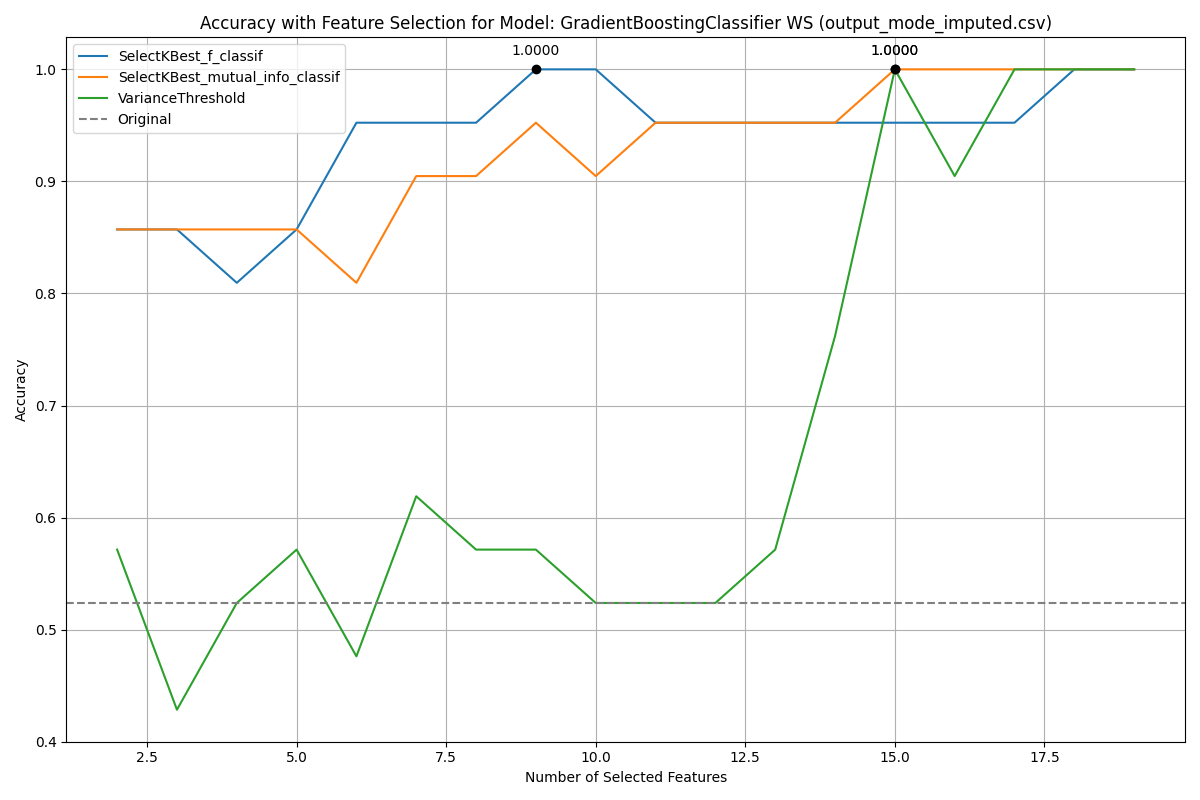
\includegraphics[width=\textwidth]{class_specific_section/images_class_ensemble_reduction/feature_selection_accuracy_plot_output_mode_imputedcsv_GradientBoostingClassifier_WS.png}
        \caption{WS}
        \label{fig_class_spec:ws_featred_graph}
    \end{minipage}
\end{figure}

\begin{figure}[H]
    \centering
    \begin{minipage}[b]{0.45\textwidth}
        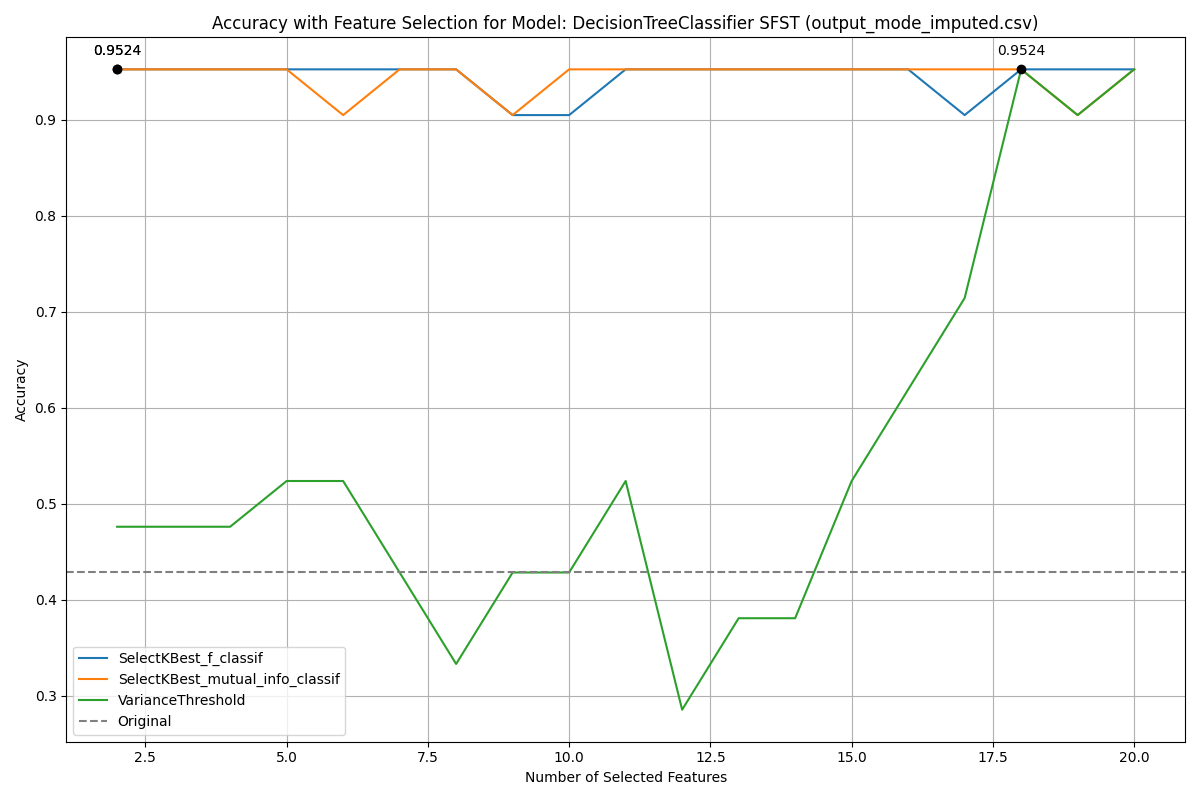
\includegraphics[width=\textwidth]{class_specific_section/images_class_ensemble_reduction/feature_selection_accuracy_plot_output_mode_imputedcsv_DecisionTreeClassifier_SFST.png}
        \caption{SFST}
        \label{fig_class_spec:sfst_featred_graph}
    \end{minipage}
    \hfill
    \begin{minipage}[b]{0.45\textwidth}
        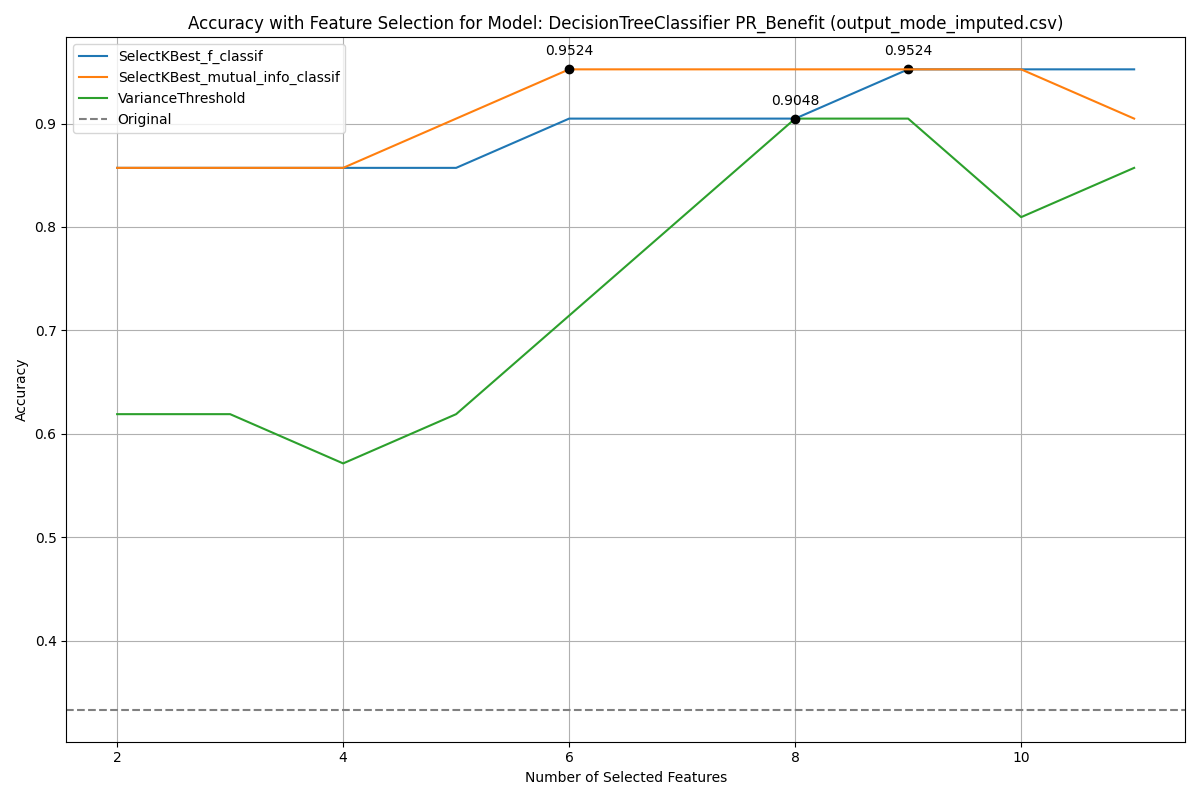
\includegraphics[width=\textwidth]{class_specific_section/images_class_ensemble_reduction/feature_selection_accuracy_plot_output_mode_imputedcsv_DecisionTreeClassifier_PR_Benefit.png}
        \caption{PR Benefit}
        \label{fig_class_spec:pr_ben_featred_graph}
    \end{minipage}
\end{figure}

\begin{figure}[H]
    \centering
    \begin{minipage}[b]{0.45\textwidth}
        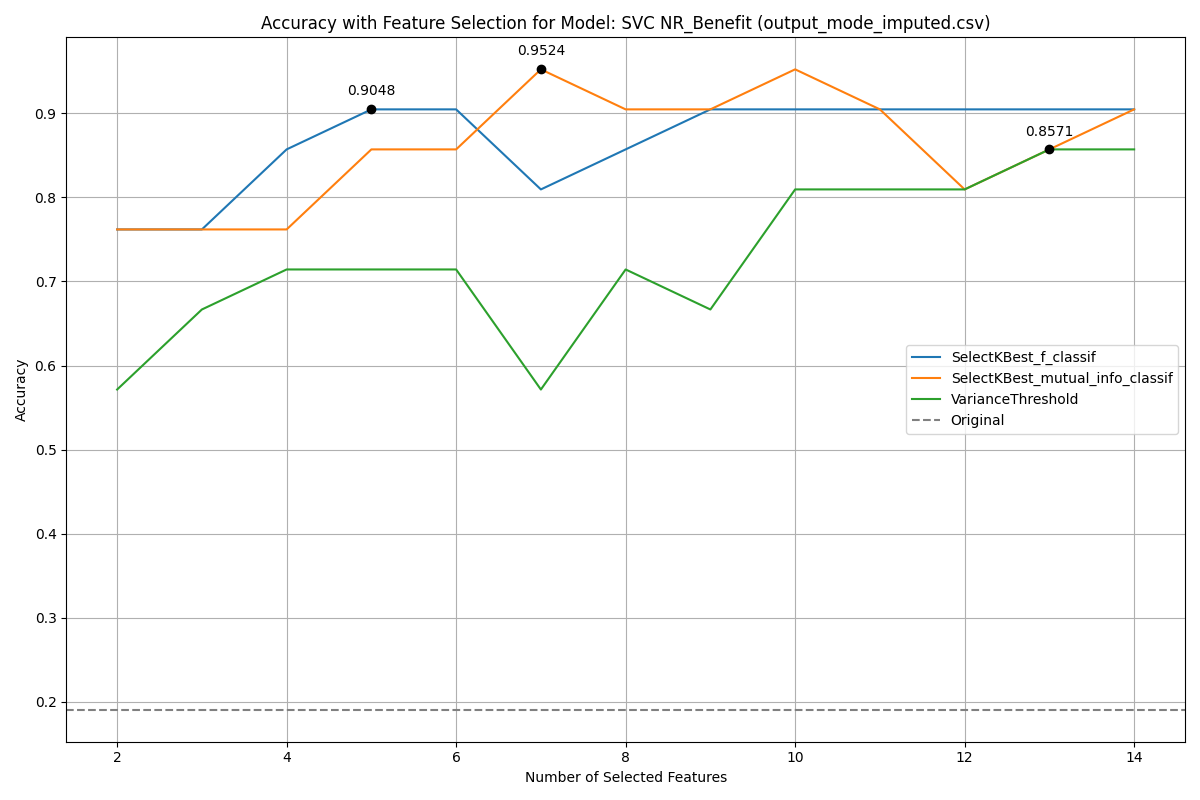
\includegraphics[width=\textwidth]{class_specific_section/images_class_ensemble_reduction/feature_selection_accuracy_plot_output_mode_imputedcsv_SVC_NR_Benefit.png}
        \caption{NR Benefit}
        \label{fig_class_spec:nr_ben_featred_graph}
    \end{minipage}
    \hfill
    \begin{minipage}[b]{0.45\textwidth}
        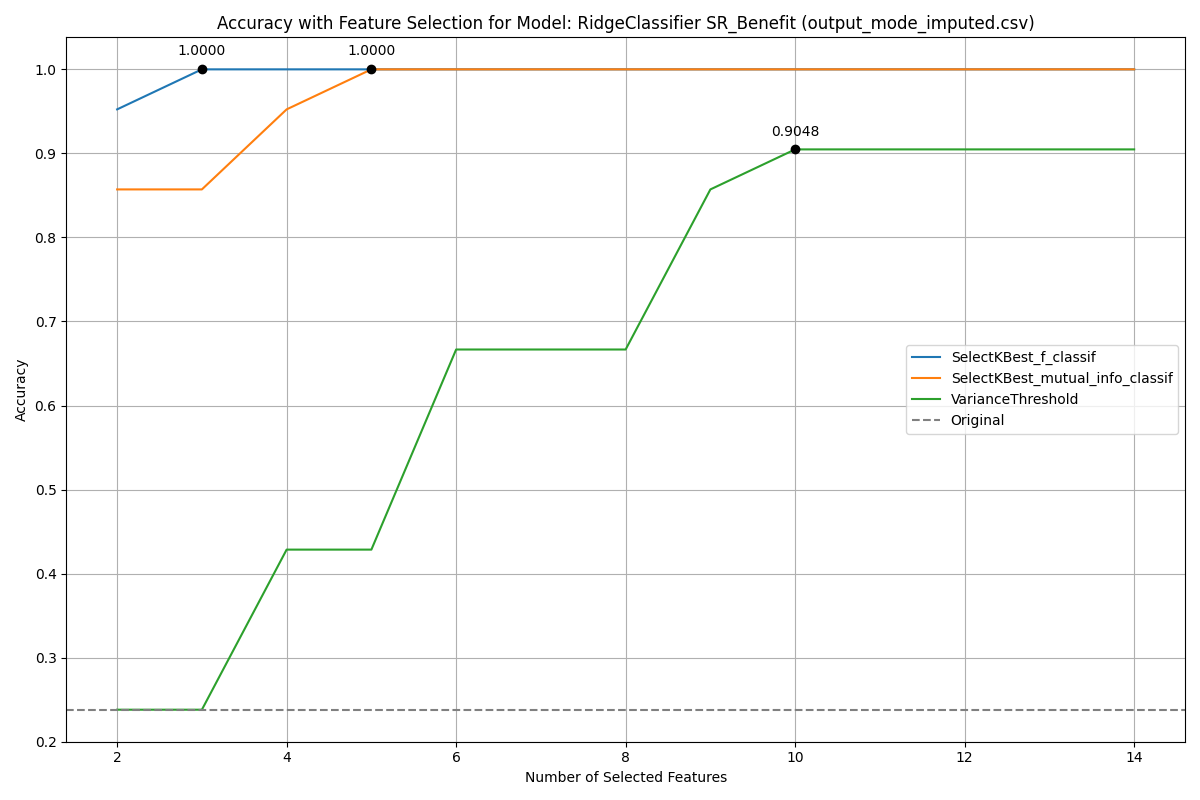
\includegraphics[width=\textwidth]{class_specific_section/images_class_ensemble_reduction/feature_selection_accuracy_plot_output_mode_imputedcsv_RidgeClassifier_SR_Benefit.png}
        \caption{SR Benefit}
        \label{fig_class_spec:sr_ben_featred_graph}
    \end{minipage}
\end{figure}

\begin{figure}[H]
    \centering
    \begin{minipage}[b]{0.45\textwidth}
        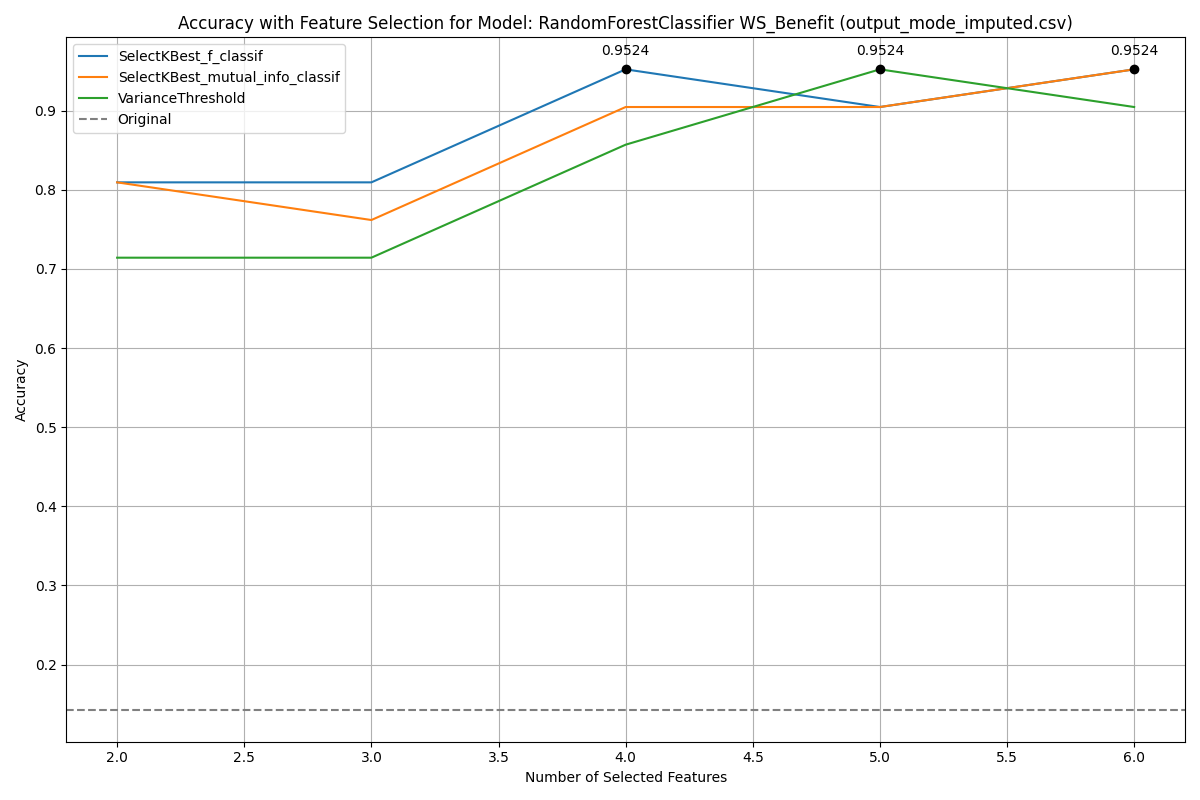
\includegraphics[width=\textwidth]{class_specific_section/images_class_ensemble_reduction/feature_selection_accuracy_plot_output_mode_imputedcsv_RandomForestClassifier_WS_Benefit.png}
        \caption{WS Benefit}
        \label{fig_class_spec:ws_ben_featred_graph}
    \end{minipage}
    \hfill
    \begin{minipage}[b]{0.45\textwidth}
        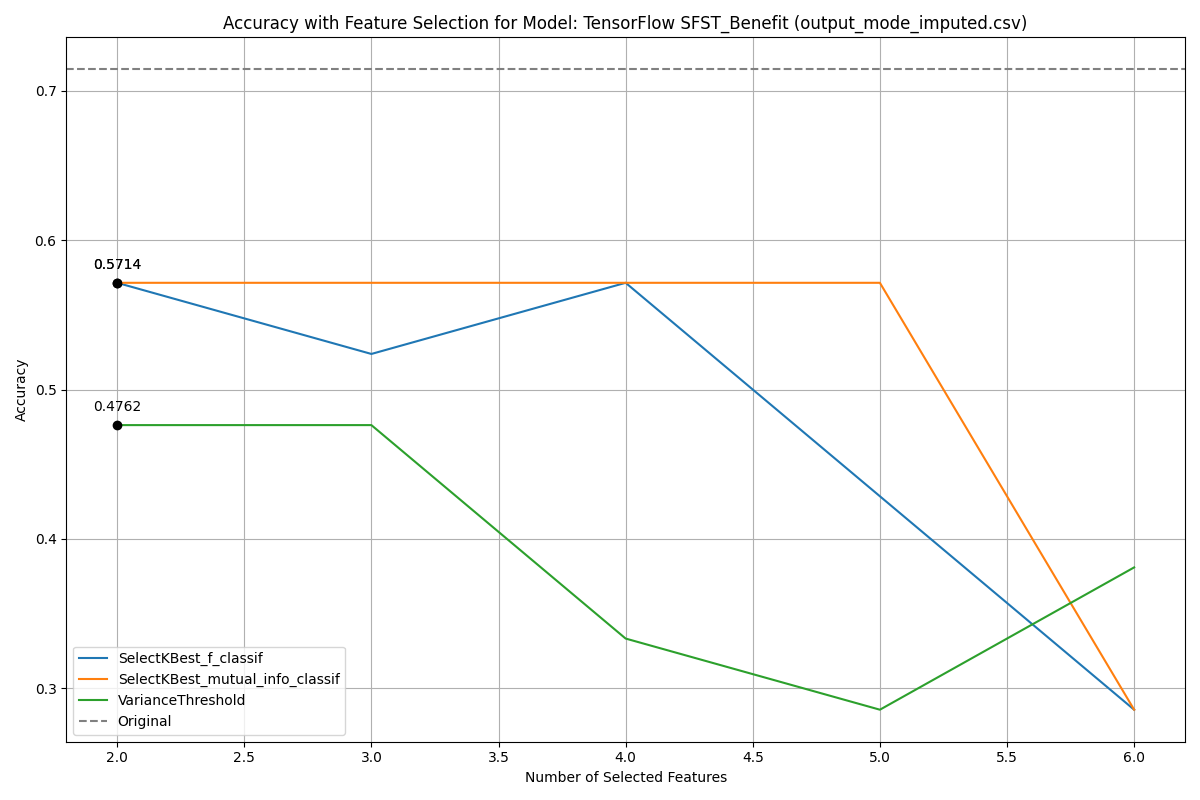
\includegraphics[width=\textwidth]{class_specific_section/images_class_ensemble_reduction/feature_selection_accuracy_plot_output_mode_imputedcsv_TensorFlow_SFST_Benefit.png}
        \caption{SFST Benefit}
        \label{fig_class_spec:sfst_ben_featred_graph}
    \end{minipage}
\end{figure}





\subsection{Regression Models}\label{sec:reg}
\subsubsection{All Features}
\begin{table}[H]
\centering
\begin{tabular}{|c|c|c|c|c|}
\hline
\textbf{Feature} & \textbf{NNorm MSE} & \textbf{Norm MSE} & \textbf{Model} & \textbf{Dataset} \\
\hline
NR & 0.17 & 0.48 & AdaBoostRegressor & Interpolated \\
\hline
PR & 0.12 & 0.19 & AdaBoostRegressor & custom \\
\hline
SR & 0.37 & 0.62 & AdaBoostRegressor & bfill \\
\hline
SFST & 0.20 & 0.33 & AdaBoostRegressor & ffill \\
\hline
WS & 0.25 & 0.49 & AdaBoostRegressor & knn \\
\hline
NR Benefit & 0.39 & 0.45 & MLPRegressor & ffill \\
\hline
PR Benefit & 0.22 & 0.23 & SGDRegressor & iterative \\
\hline
SR Benefit & 0.17 & 0.22 & AdaBoostRegressor & bfill \\
\hline
SFST Benefit & 0.51 & 0.98 & AdaBoostRegressor & custom \\
\hline
WS Benefit & 1.19 & 1.21 & AdaBoostRegressor & bfill \\
\hline
\end{tabular}
\caption{Best MSE for Non-Normalized and Normalized Data with Algorithm and Dataset}
\label{reg_all_tab:norm_mse}
\end{table}


\begin{table}[H]
\centering
\begin{tabular}{|c|c|c|c|}
\hline
\textbf{Feature} & \textbf{PNorm MSE} & \textbf{Model} & \textbf{Dataset}  \\
\hline
NR & 0.31& AdaBoostRegressor & knn  \\
\hline
PR  & 0.21 & AdaBoostRegressor & iterative\\
\hline
SR & 0.46 & AdaBoostRegressor & knn \\
\hline
SFST & 0.26& AdaBoostRegressor & custom  \\
\hline
WS & 0.60 & AdaBoostRegressor & custom \\
\hline
NR Benefit & 0.28& MLPRegressor & knn  \\
\hline
PR Benefit  & 0.49 \& MLPRegressor & ffill \\
\hline
SR Benefit & 0.07& SGDRegressor & mode  \\
\hline
SFST Benefit & 0.71& AdaBoostRegressor & iterative  \\
\hline
WS Benefit & 0.63& AdaBoostRegressor & mean  \\
\hline
\end{tabular}
\caption{Best MSE for Pre-Normalized Data}
\label{reg_all_tab:pre_norm_mse}
\end{table}

\begin{figure}[H]
    \centering
    \begin{minipage}{0.45\textwidth}
        \centering
        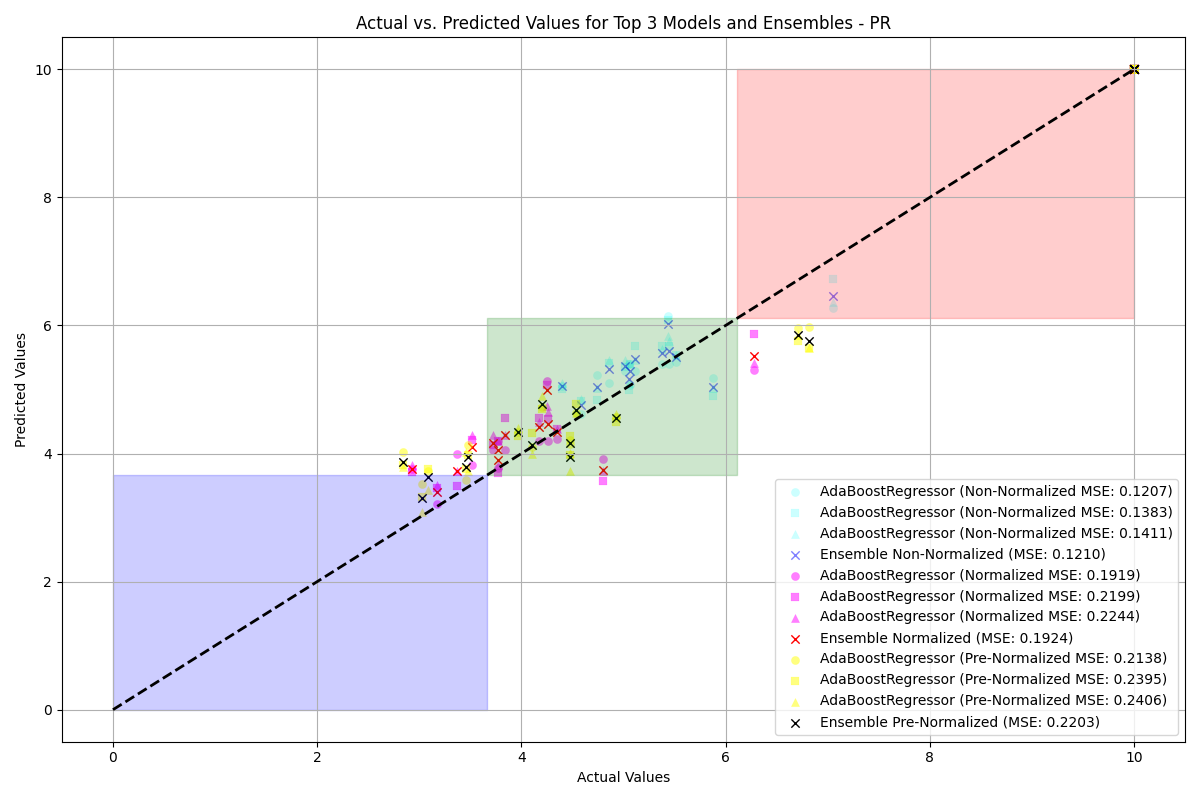
\includegraphics[width=\linewidth]{reg_section_all/ensemble_learning/actual_vs_predicted_top_3_models_and_ensembles_PR.png}
        \caption{PR}
        \label{reg_all_fig:pr_ensemble}
    \end{minipage}\hfill
    \begin{minipage}{0.45\textwidth}
        \centering
        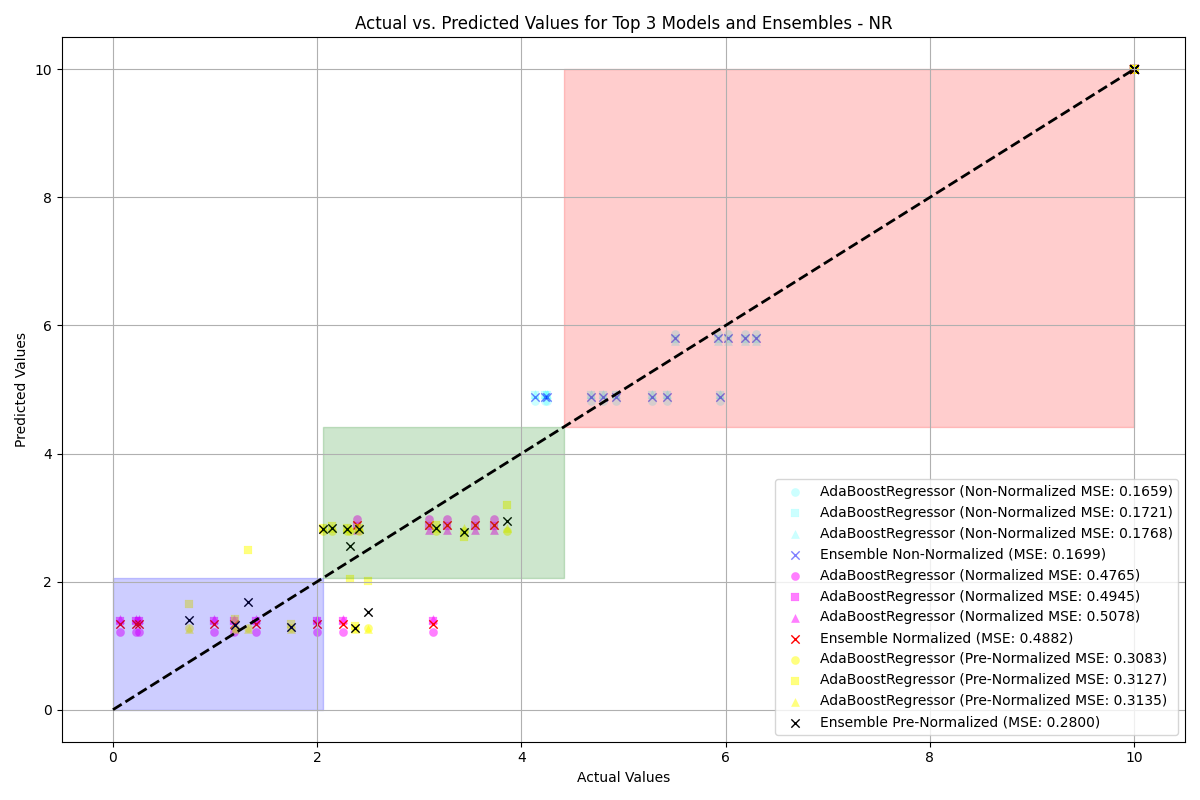
\includegraphics[width=\linewidth]{reg_section_all/ensemble_learning/actual_vs_predicted_top_3_models_and_ensembles_NR.png}
        \caption{NR}
        \label{reg_all_fig:nr_ensemble}
    \end{minipage}
\end{figure}

\begin{figure}[H]
    \centering
    \begin{minipage}{0.45\textwidth}
        \centering
        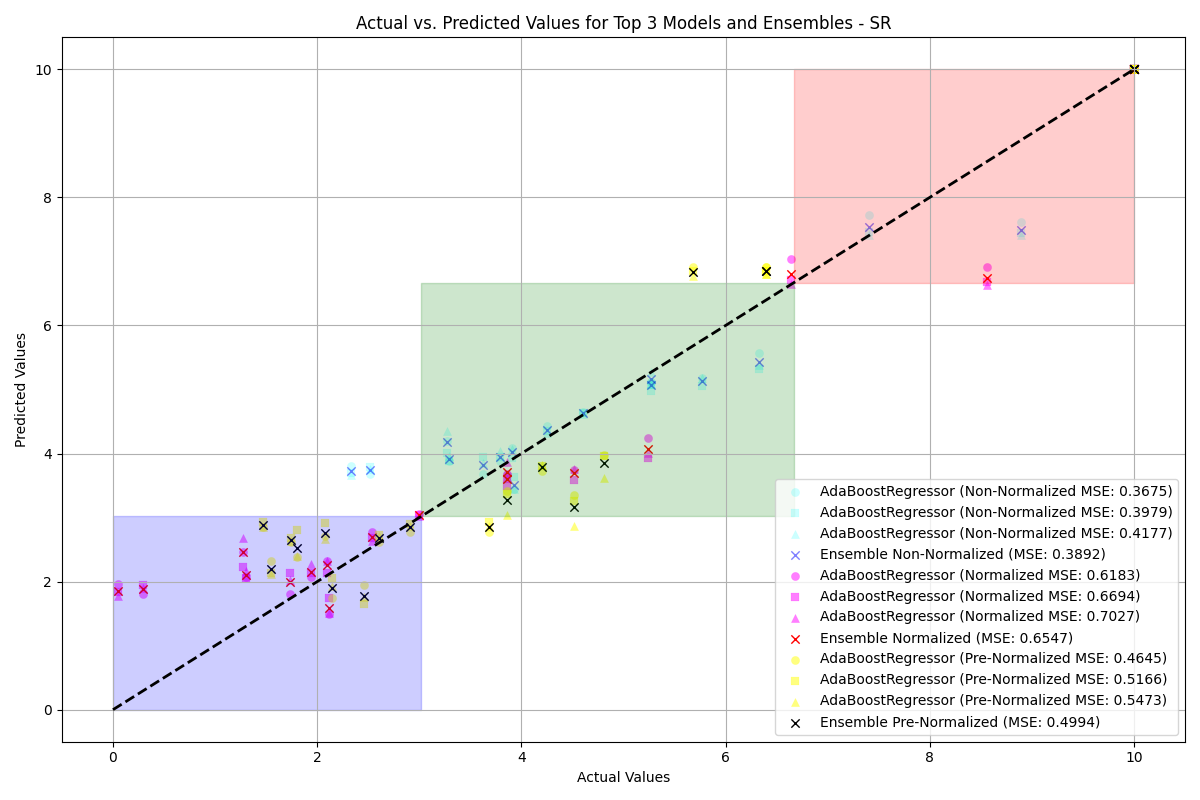
\includegraphics[width=\linewidth]{reg_section_all/ensemble_learning/actual_vs_predicted_top_3_models_and_ensembles_SR.png}
        \caption{SR}
        \label{reg_all_fig:sr_ensemble}
    \end{minipage}\hfill
    \begin{minipage}{0.45\textwidth}
        \centering
        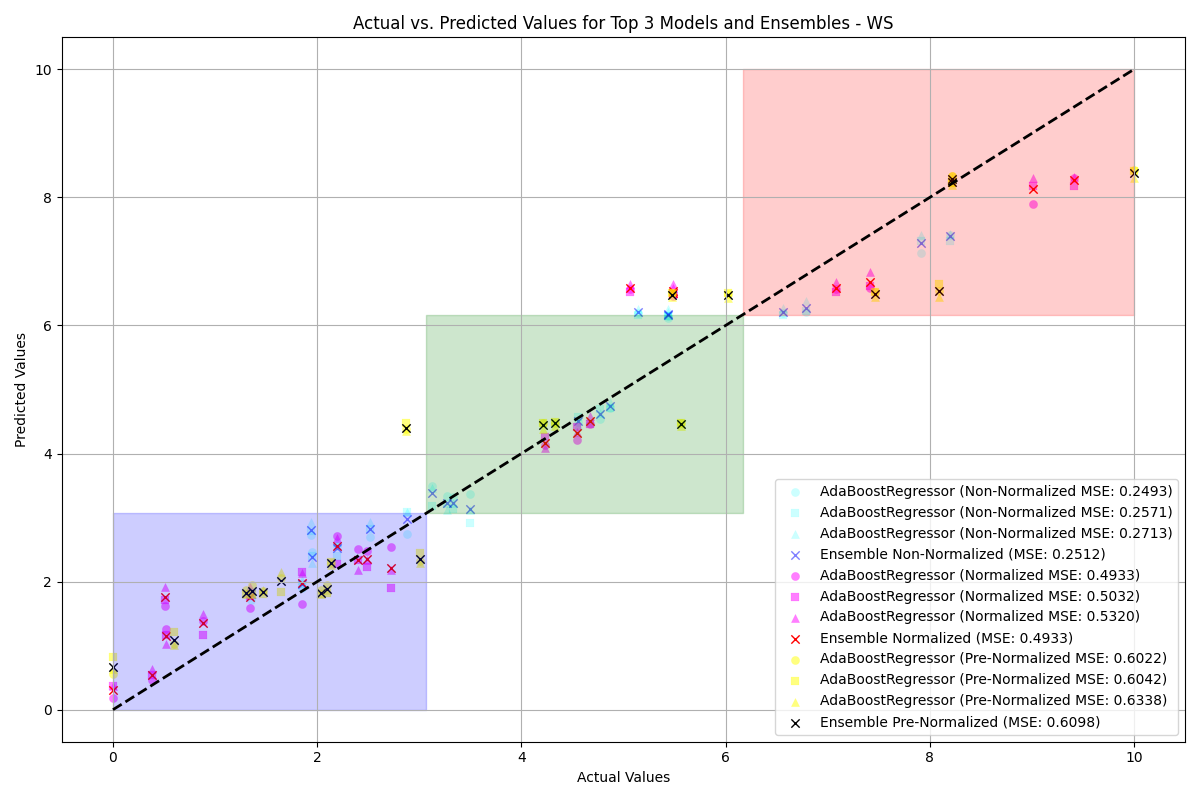
\includegraphics[width=\linewidth]{reg_section_all/ensemble_learning/actual_vs_predicted_top_3_models_and_ensembles_WS.png}
        \caption{WS}
        \label{reg_all_fig:ws_ensemble}
    \end{minipage}
\end{figure}

\begin{figure}[H]
    \centering
    \begin{minipage}{0.45\textwidth}
        \centering
        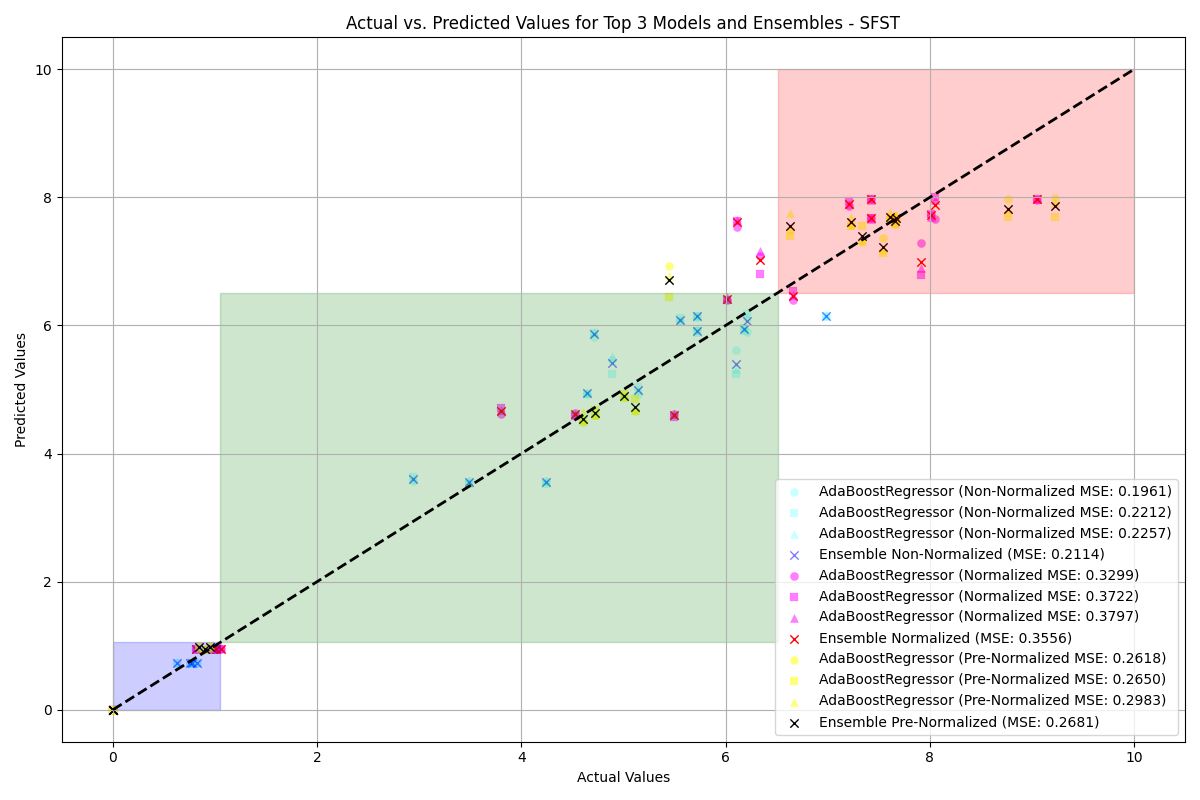
\includegraphics[width=\linewidth]{reg_section_all/ensemble_learning/actual_vs_predicted_top_3_models_and_ensembles_SFST.png}
        \caption{SFST}
        \label{reg_all_fig:sfst_ensemble}
    \end{minipage}\hfill
    \begin{minipage}{0.45\textwidth}
        \centering
        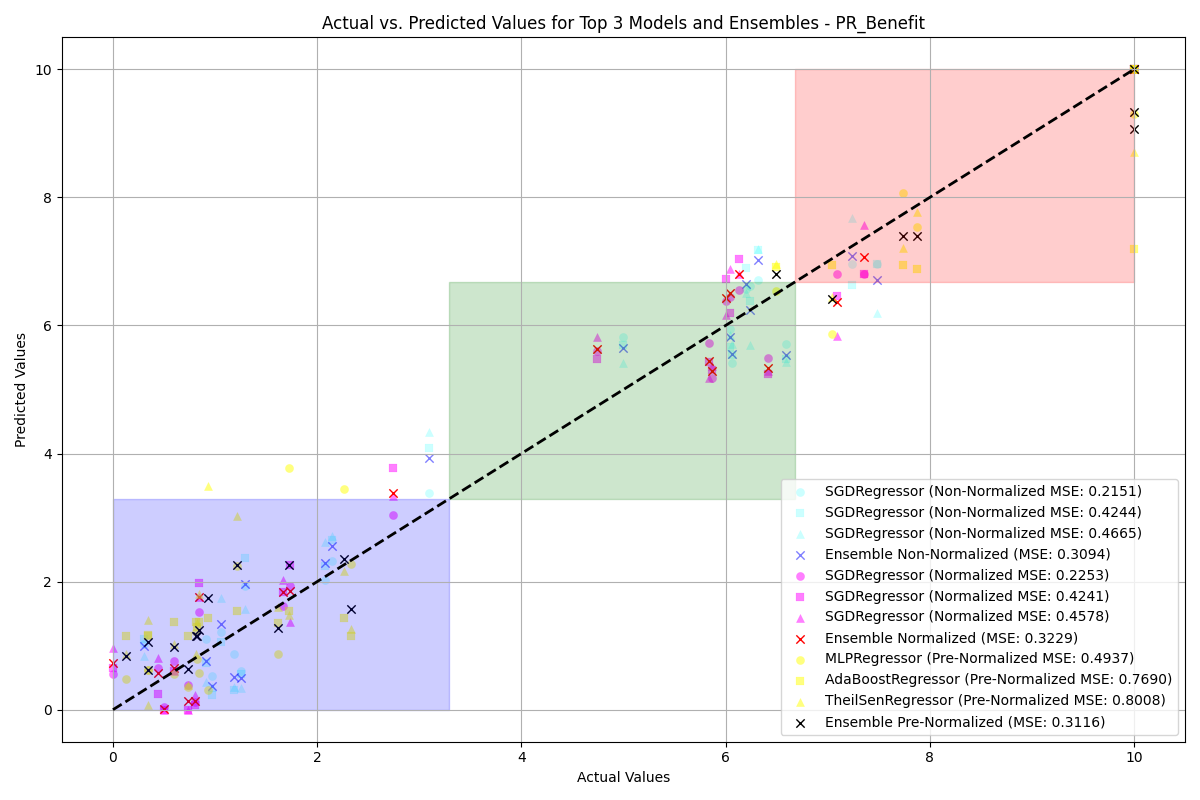
\includegraphics[width=\linewidth]{reg_section_all/ensemble_learning/actual_vs_predicted_top_3_models_and_ensembles_PR_Benefit.png}
        \caption{PR Benefit}
        \label{reg_all_fig:pr_ben_ensemble}
    \end{minipage}
\end{figure}

\begin{figure}[H]
    \centering
    \begin{minipage}{0.45\textwidth}
        \centering
        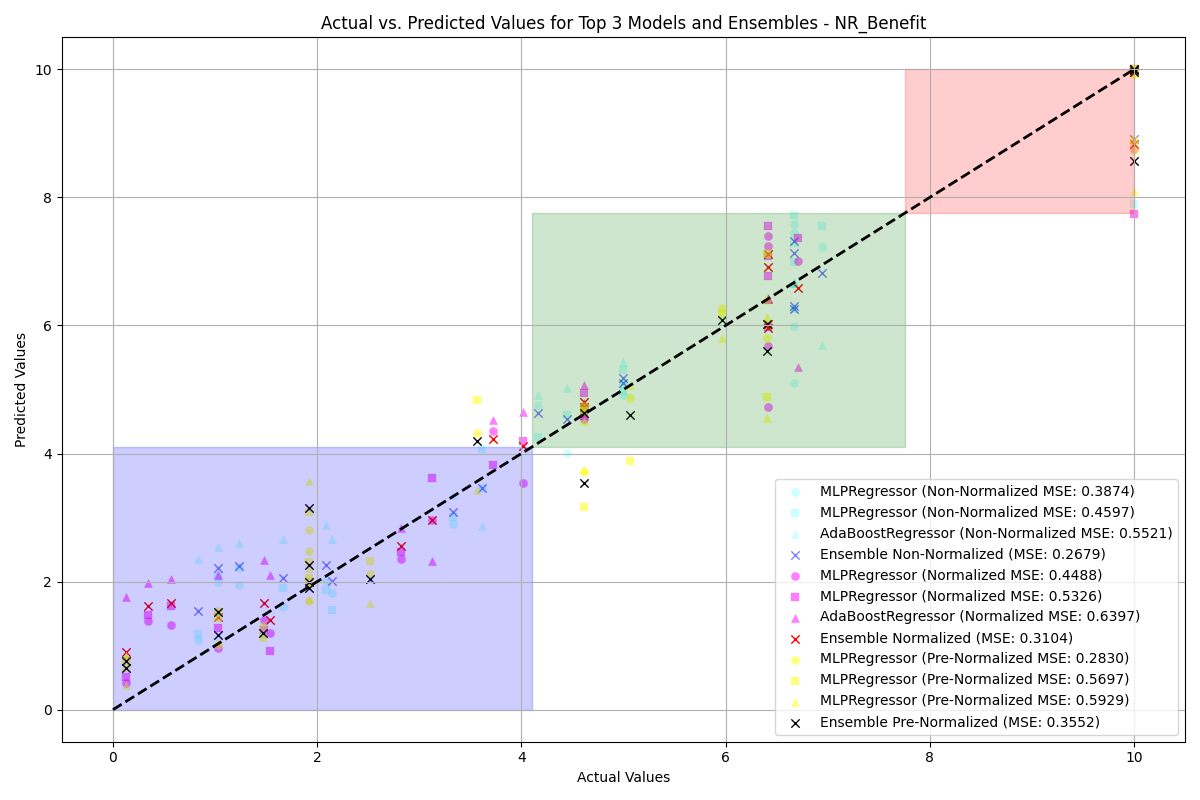
\includegraphics[width=\linewidth]{reg_section_all/ensemble_learning/actual_vs_predicted_top_3_models_and_ensembles_NR_Benefit.png}
        \caption{NR Benefit}
        \label{reg_all_fig:nr_ben_ensemble}
    \end{minipage}\hfill
    \begin{minipage}{0.45\textwidth}
        \centering
        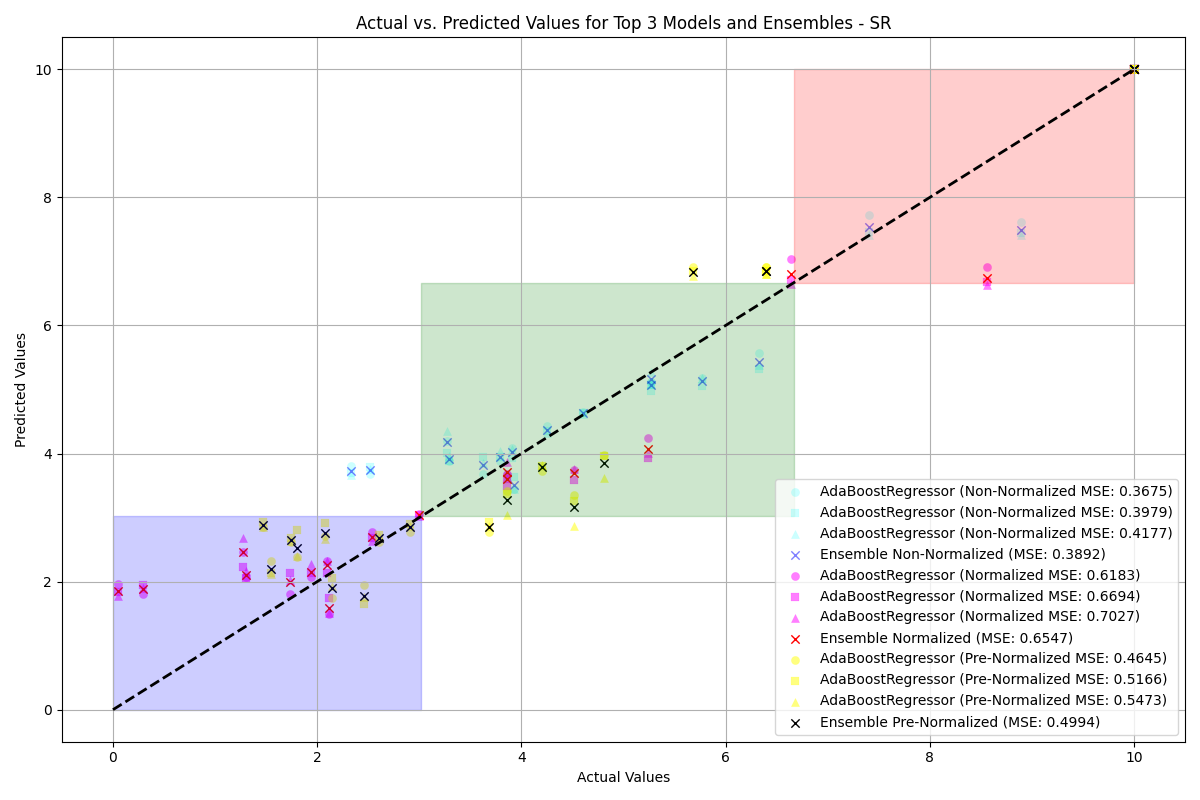
\includegraphics[width=\linewidth]{reg_section_all/ensemble_learning/actual_vs_predicted_top_3_models_and_ensembles_SR.png}
        \caption{SR Benefit}
        \label{reg_all_fig:sr_ben_ensemble}
    \end{minipage}
\end{figure}

\begin{figure}[H]
    \centering
    \begin{minipage}{0.45\textwidth}
        \centering
        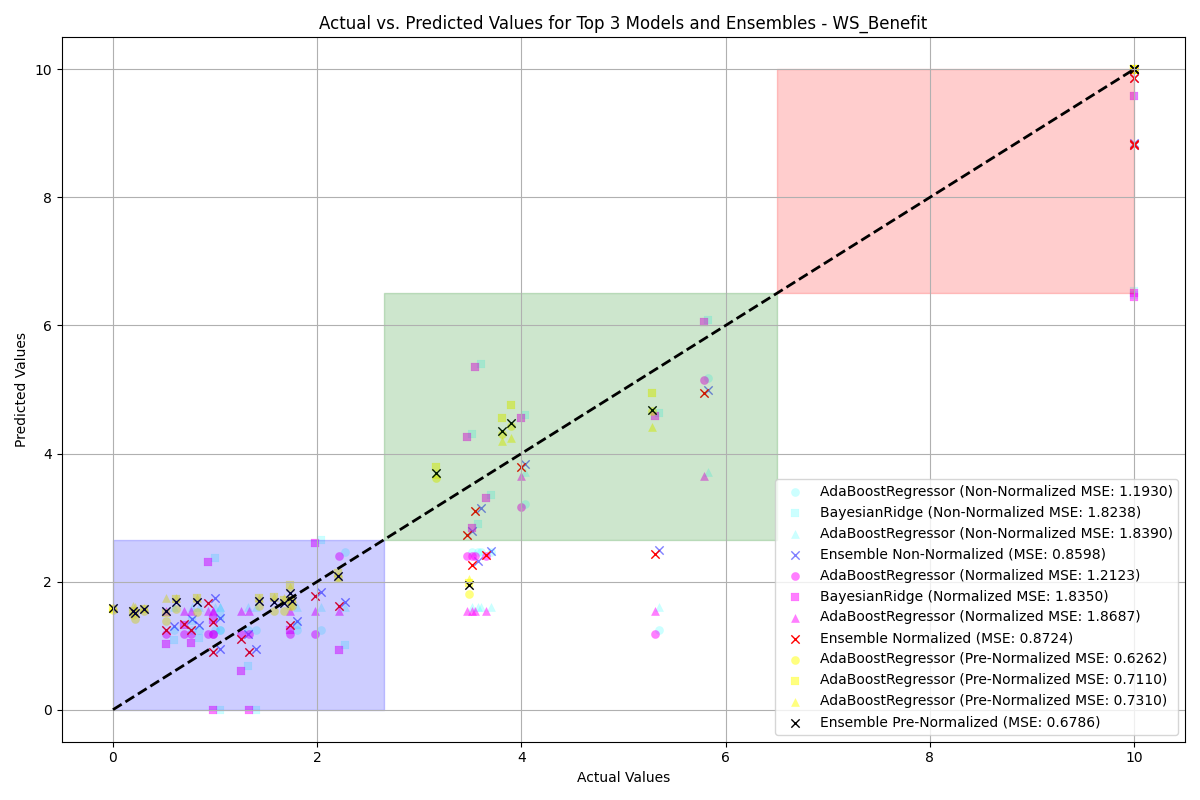
\includegraphics[width=\linewidth]{reg_section_all/ensemble_learning/actual_vs_predicted_top_3_models_and_ensembles_WS_Benefit.png}
        \caption{WS Benefit}
        \label{reg_all_fig:ws_ben_ensemble}
    \end{minipage}\hfill
    \begin{minipage}{0.45\textwidth}
        \centering
        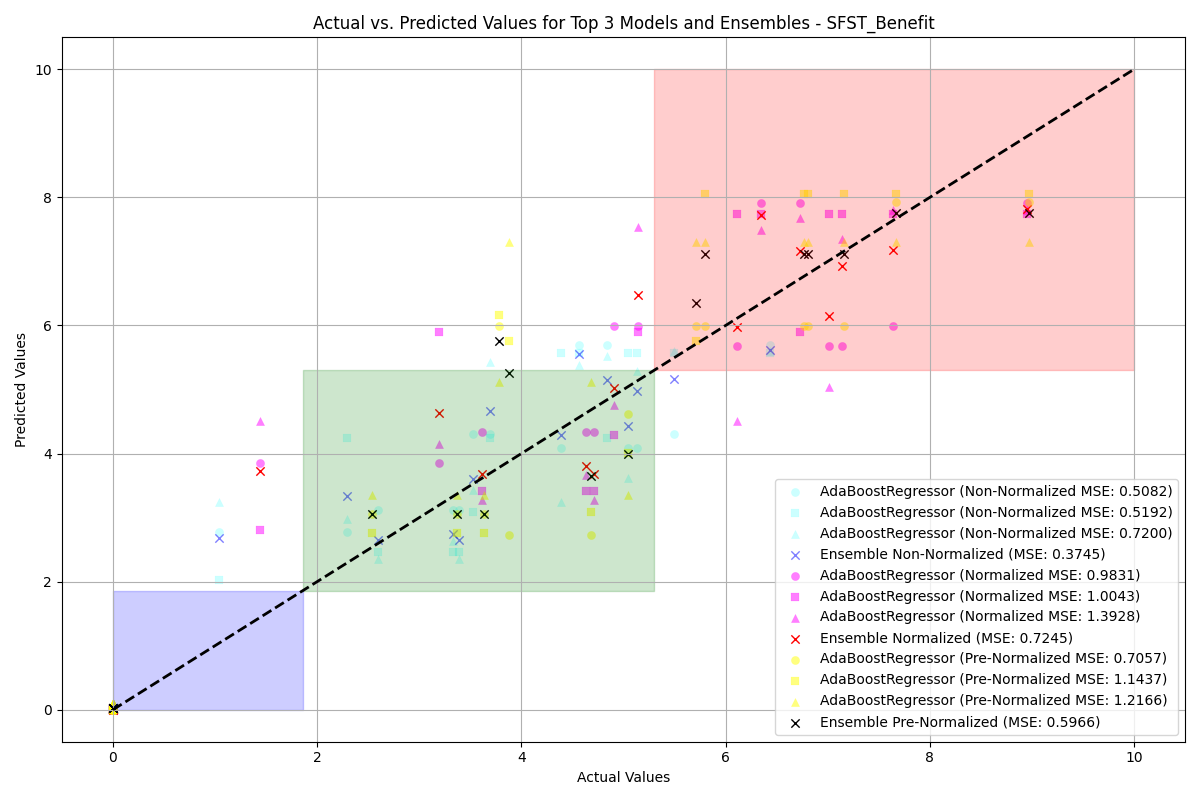
\includegraphics[width=\linewidth]{reg_section_all/ensemble_learning/actual_vs_predicted_top_3_models_and_ensembles_SFST_Benefit.png}
        \caption{SFST Benefit}
        \label{reg_all_fig:sfst_ben_ensemble}
    \end{minipage}
\end{figure}

\begin{longtable}{|p{2cm}|p{2cm}|p{2cm}|p{2cm}|p{2cm}|p{4cm}|}
\hline
\textbf{Model} & \textbf{Lower Acc.} & \textbf{Moderate Acc.} & \textbf{Higher Acc.} & \textbf{Overall Acc.} & \textbf{Top Features} \\ \hline
\endfirsthead
\hline
\textbf{Model} & \textbf{Lower Acc.} & \textbf{Moderate Acc.} & \textbf{Higher Acc.} & \textbf{Overall Acc.} & \textbf{Top Features} \\ \hline
\endhead

WS & 80.81\% & 64.20\% & 70.37\% & 74.07\% & Provincial\_Class, Hydrogeomorphic\_Class, OF22, F22, F28, F31, F43, F44, F45 \\ \hline
PR & 13.89\% & 77.78\% & 87.50\% & 69.31\% & Provincial\_Class, Federal\_Class, F43, F44, F45 \\ \hline
NR & 32.80\% & 65.08\% & 76.19\% & 58.02\% & Provincial\_Class, F24, F43, F44, F45 \\ \hline
SR & 62.22\% & 60.00\% & 62.35\% & 61.73\% & F28, F29, F31, F44, F45 \\ \hline
SFST & 56.17\% & 60.85\% & 76.39\% & 65.43\% & F1, F43 \\ \hline
WS Benefit & 68.35\% & 46.56\% & 44.44\% & 57.67\% & Hydrogeomorphic\_Class, OF17, OF18, OF23, OF24, F51 \\ \hline
PR Benefit & 80.00\% & 44.97\% & 29.63\% & 58.73\% & Regime, Moss\_Cover, Living\_Moss\_Depth, OF19, OF20, OF21, OF22, OF24, F41 \\ \hline
NR Benefit & 70.74\% & 80.42\% & 49.07\% & 69.84\% & Living\_Moss\_Depth, OF9, OF10, OF19, OF20, OF21, OF22, OF23, F41 \\ \hline
SR Benefit & 93.70\% & 53.91\% & 0.00\% & 67.72\% & Provincial\_Class, Federal\_Class, Regime, Vegetation\_Type, Living\_Moss\_Depth, Organic\_Depth, Hydrogeomorphic\_Class, OF18, OF24, F41 \\ \hline
SFST Benefit & 59.72\% & 32.10\% & 48.15\% & 47.97\% & Provincial\_Class, Federal\_Class, Moss\_Cover, Surface\_Water\_Present, Hydrogeomorphic\_Class, OF18, OF22, OF25, OF28 \\ \hline
\caption{Classification Accuracies and Top Features for Various Models}
\label{tab:grouping_1d}
\end{longtable}

\begin{longtable}{|p{1.5cm}|p{2.0cm}|p{2.0cm}|p{2.0cm}|p{2.0cm}|p{4cm}|}
\hline
\textbf{Model} & \textbf{Lower Acc.} & \textbf{Moderate Acc.} & \textbf{Higher Acc.} & \textbf{Overall Acc.} & \textbf{Top Features} \\ \hline
\endfirsthead
\hline
\textbf{Model} & \textbf{Lower Acc.} & \textbf{Moderate Acc.} & \textbf{Higher Acc.} & \textbf{Overall Acc.} & \textbf{Top Features} \\ \hline
\endhead

WS & 100.00\% & 50.00\% & 100.00\% & 85.71\% & F22, F31, F43, F44, F46, F5, OF18, OF27 \\ \hline
PR & 0.00\% & 100.00\% & 100.00\% & 76.19\% & F43, F44, F45, F5, OF18, OF27 \\ \hline
NR & 0.00\% & 71.43\% & 42.86\% & 80.95\% & F43, F44, F45, F5, OF18, OF27, OF34, S4 \\ \hline
SR & 30.00\% & 80.00\% & 50.00\% & 90.48\% & F24, F28, F31, F43, F44, F45, F5, OF18, OF27 \\ \hline
SFST & 100.00\% & 42.86\% & 100.00\% & 80.95\% & F43, F44, F45, F46, OF18, OF27 \\ \hline
WS Benefit & 54.55\% & 71.43\% & 66.67\% & 90.48\% & F5, OF17, OF18, OF23, OF27, OF34, S4 \\ \hline
PR Benefit & 100.00\% & 85.71\% & 25.00\% & 80.95\% & F14, F3\_c, F41, F44, OF18, OF19, OF27 \\ \hline
NR Benefit & 100.00\% & 85.71\% & 50.00\% & 85.71\% & F41, F5, OF10, OF18, OF19, OF22, OF27, OF9 \\ \hline
SR Benefit & 100.00\% & 0.00\% & 0.00\% & 85.71\% & F12, F41, OF18, OF22, OF27, OF30 \\ \hline
SFST Benefit & 37.50\% & 100.00\% & 42.86\% & 80.95\% & F12, F43, F44, F45, F5, OF18, OF27, OF30 \\ \hline
\caption{Ensemble Model Accuracies}
\label{tab:grouping_2d}
\end{longtable}

\begin{longtable}{|p{1.5cm}|p{2.0cm}|p{2.0cm}|p{2.0cm}|p{2.0cm}|p{4cm}|}
\hline
\textbf{Model} & \textbf{Lower Acc.} & \textbf{Moderate Acc.} & \textbf{Higher Acc.} & \textbf{Overall Acc.} & \textbf{Top Features} \\ \hline
\endfirsthead
\hline
\textbf{Model} & \textbf{Lower Acc.} & \textbf{Moderate Acc.} & \textbf{Higher Acc.} & \textbf{Overall Acc.} & \textbf{Top Features} \\ \hline
\endhead

WS & 100.00\% & 50.00\% & 75.00\% & 85.71\% & F22, F31, F43, F44, F46, F5, OF18, OF27 \\ \hline
PR & 0.00\% & 100.00\% & 100.00\% & 76.19\% & F43, F44, F45, F5, OF18, OF27 \\ \hline
NR & 0.00\% & 85.71\% & 42.86\% & 61.90\% & F43, F44, F45, F5, OF18, OF27, OF34, S4 \\ \hline
SR & 30.00\% & 80.00\% & 33.33\% & 85.71\% & F24, F28, F31, F43, F44, F45, F5, OF18, OF27 \\ \hline
SFST & 100.00\% & 42.86\% & 100.00\% & 80.95\% & F43, F44, F45, F46, OF18, OF27 \\ \hline
WS Benefit & 36.36\% & 71.43\% & 66.67\% & 80.95\% & F5, OF17, OF18, OF23, OF27, OF34, S4 \\ \hline
PR Benefit & 100.00\% & 85.71\% & 25.00\% & 80.95\% & F14, F3\_c, F41, F44, OF18, OF19, OF27 \\ \hline
NR Benefit & 100.00\% & 85.71\% & 50.00\% & 76.19\% & F41, F5, OF10, OF18, OF19, OF22, OF27, OF9 \\ \hline
SR Benefit & 100.00\% & 0.00\% & 0.00\% & 47.62\% & F12, F41, OF18, OF22, OF27, OF30 \\ \hline
SFST Benefit & 37.50\% & 100.00\% & 42.86\% & 57.14\% & F12, F43, F44, F45, F5, OF18, OF27, OF30 \\ \hline

\caption{Voting System Accuracies}
\label{tab:grouping_3d}
\end{longtable}

\begin{figure}[H]
    \centering
    \begin{minipage}{0.45\textwidth}
        \centering
        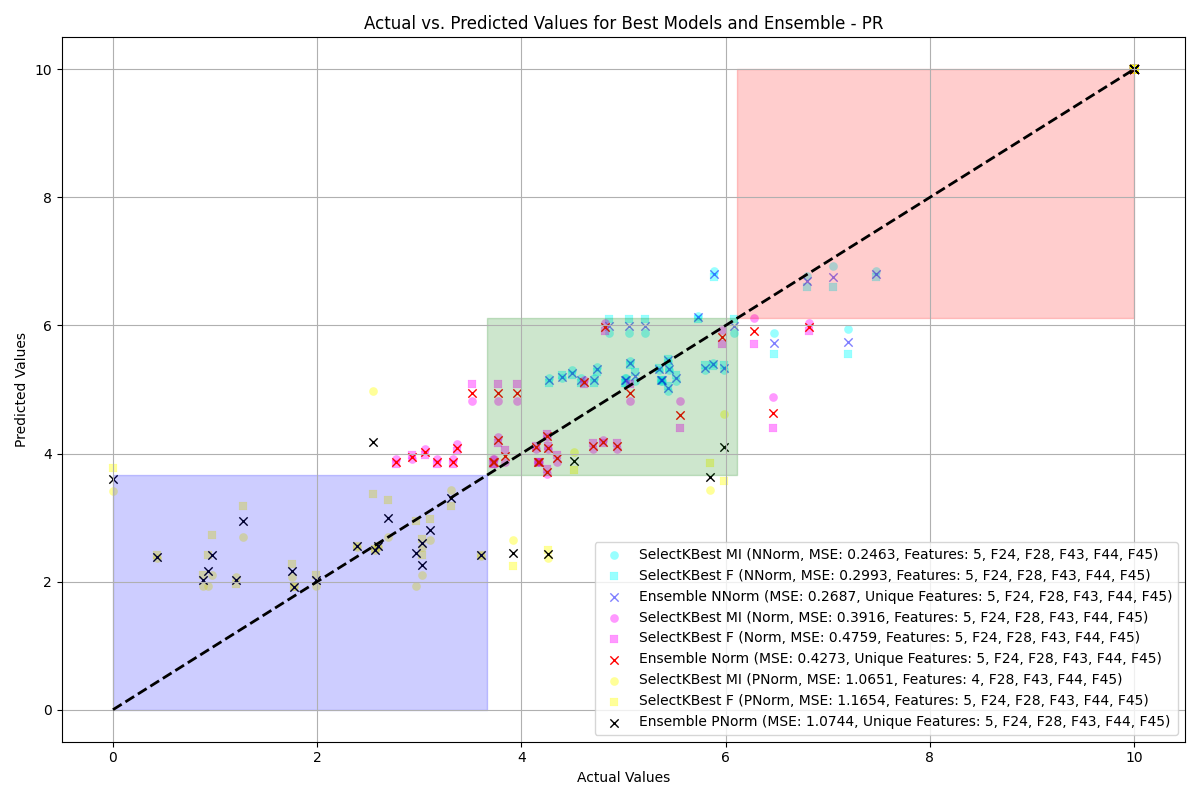
\includegraphics[width=\linewidth]{reg_section_specific/featred_ensemble_learning/actual_vs_predicted_best_feature_selection_and_ensemble_PR_10.png}
        \caption{PR}
        \label{reg_spec_fig:pr_featred}
    \end{minipage}\hfill
    \begin{minipage}{0.45\textwidth}
        \centering
        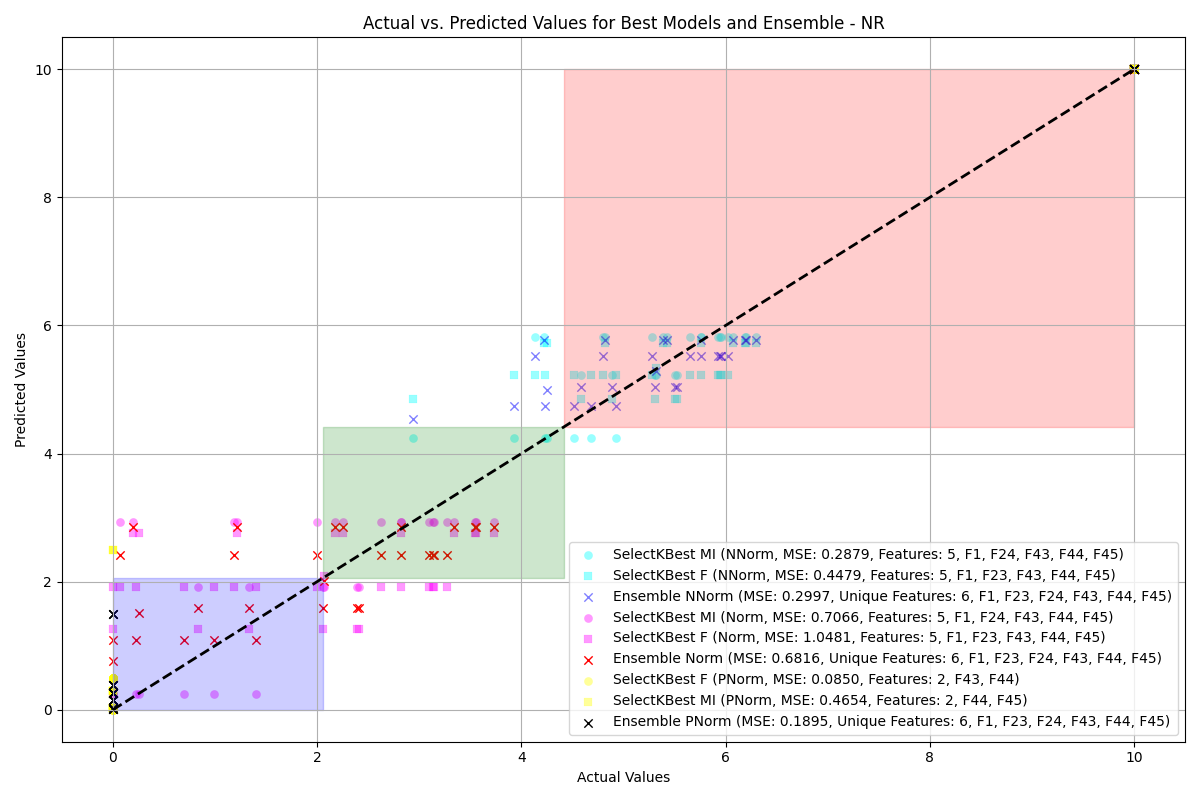
\includegraphics[width=\linewidth]{reg_section_specific/featred_ensemble_learning/actual_vs_predicted_best_feature_selection_and_ensemble_NR_10.png}
        \caption{NR}
        \label{reg_spec_fig:nr_featred}
    \end{minipage}
\end{figure}

\begin{figure}[H]
    \centering
    \begin{minipage}{0.45\textwidth}
        \centering
        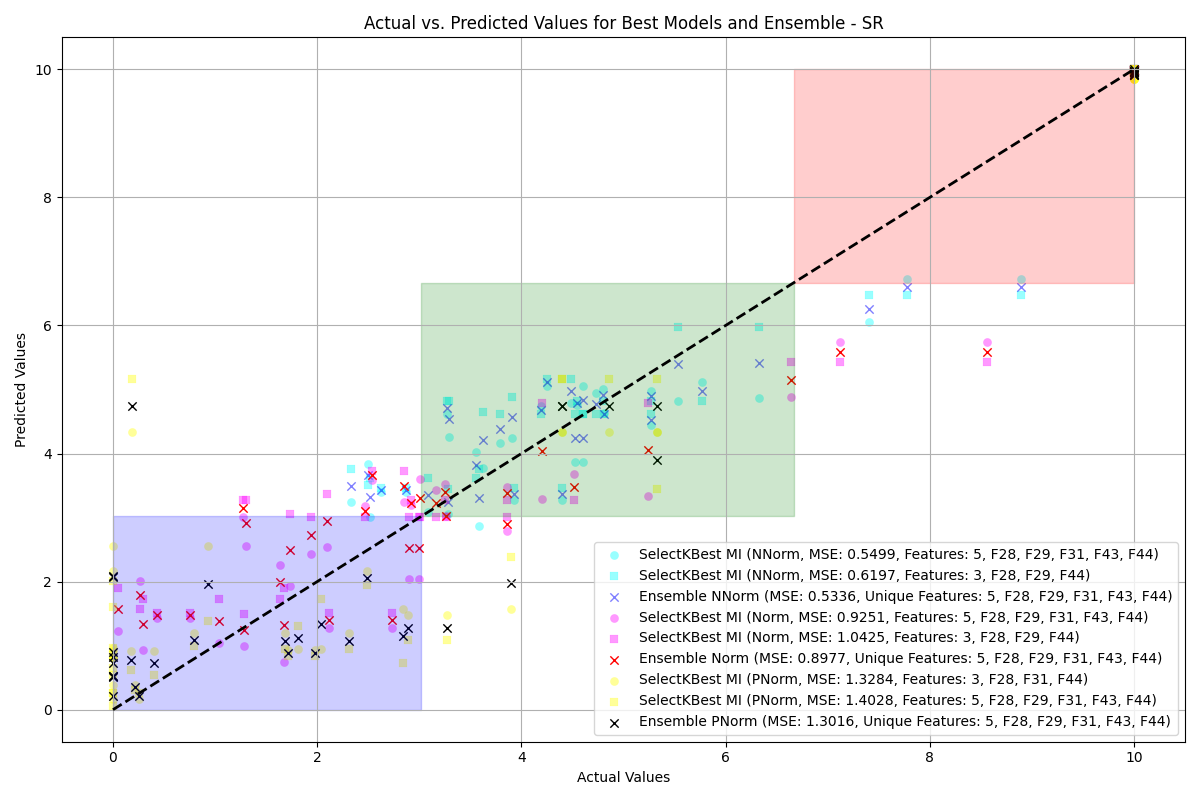
\includegraphics[width=\linewidth]{reg_section_specific/featred_ensemble_learning/actual_vs_predicted_best_feature_selection_and_ensemble_SR_10.png}
        \caption{SR}
        \label{reg_spec_fig:sr_featred}
    \end{minipage}\hfill
    \begin{minipage}{0.45\textwidth}
        \centering
        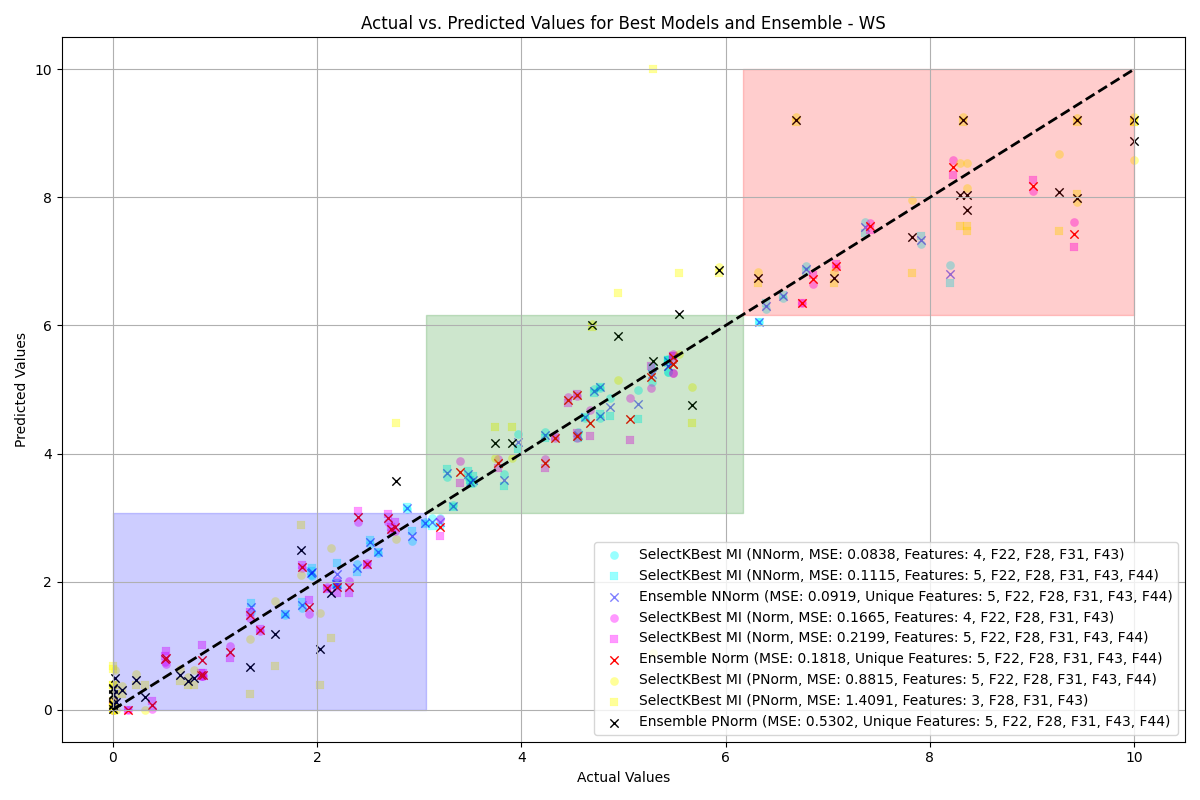
\includegraphics[width=\linewidth]{reg_section_specific/featred_ensemble_learning/actual_vs_predicted_best_feature_selection_and_ensemble_WS_10.png}
        \caption{WS}
        \label{reg_spec_fig:ws_featred}
    \end{minipage}
\end{figure}

\begin{figure}[H]
    \centering
    \begin{minipage}{0.45\textwidth}
        \centering
        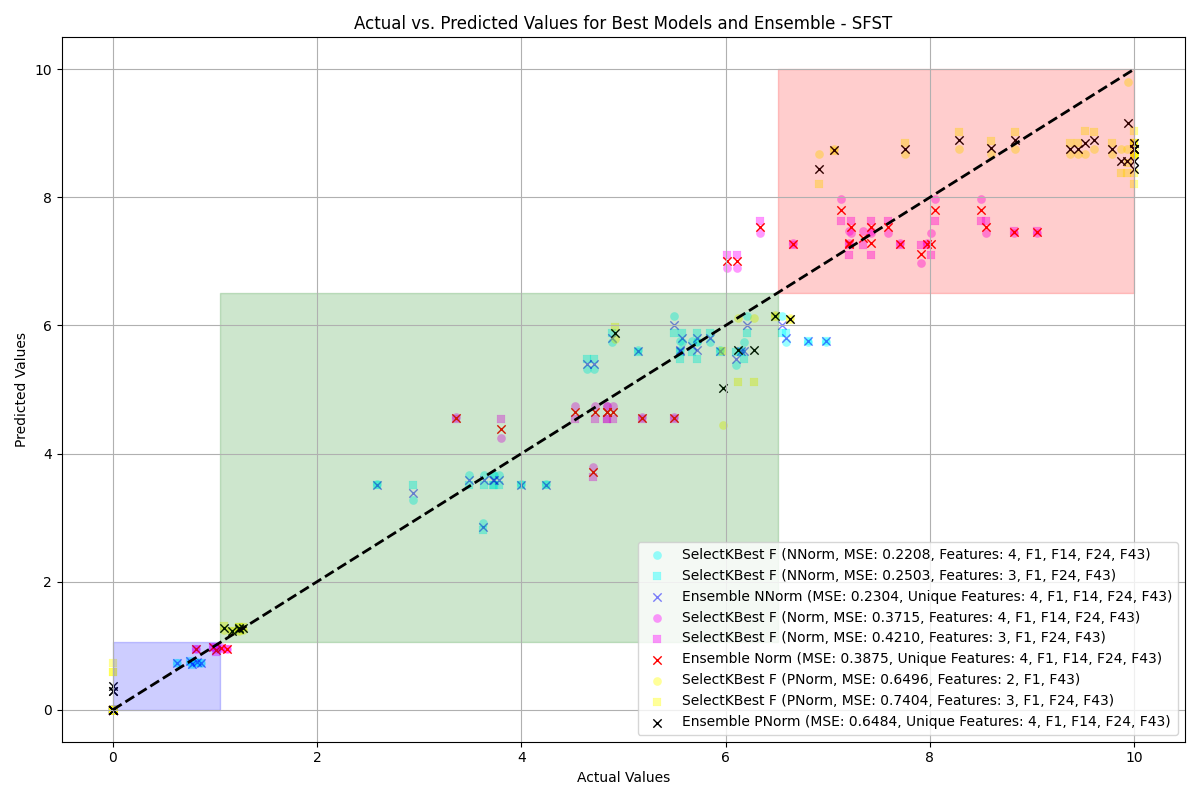
\includegraphics[width=\linewidth]{reg_section_specific/featred_ensemble_learning/actual_vs_predicted_best_feature_selection_and_ensemble_SFST_10.png}
        \caption{SFST}
        \label{reg_spec_fig:sfst_featred}
    \end{minipage}\hfill
    \begin{minipage}{0.45\textwidth}
        \centering
        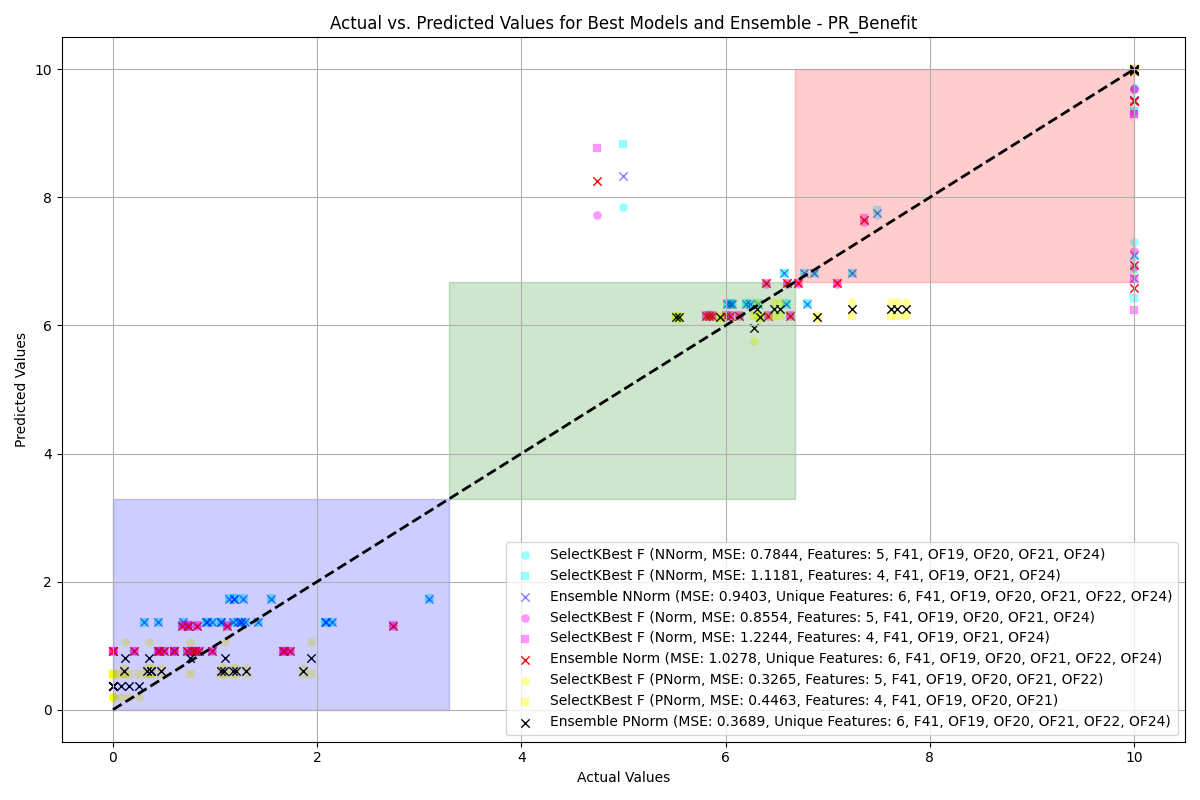
\includegraphics[width=\linewidth]{reg_section_specific/featred_ensemble_learning/actual_vs_predicted_best_feature_selection_and_ensemble_PR_Benefit_10.png}
        \caption{PR Benefit}
        \label{reg_spec_fig:pr_ben_featred}
    \end{minipage}
\end{figure}

\begin{figure}[H]
    \centering
    \begin{minipage}{0.45\textwidth}
        \centering
        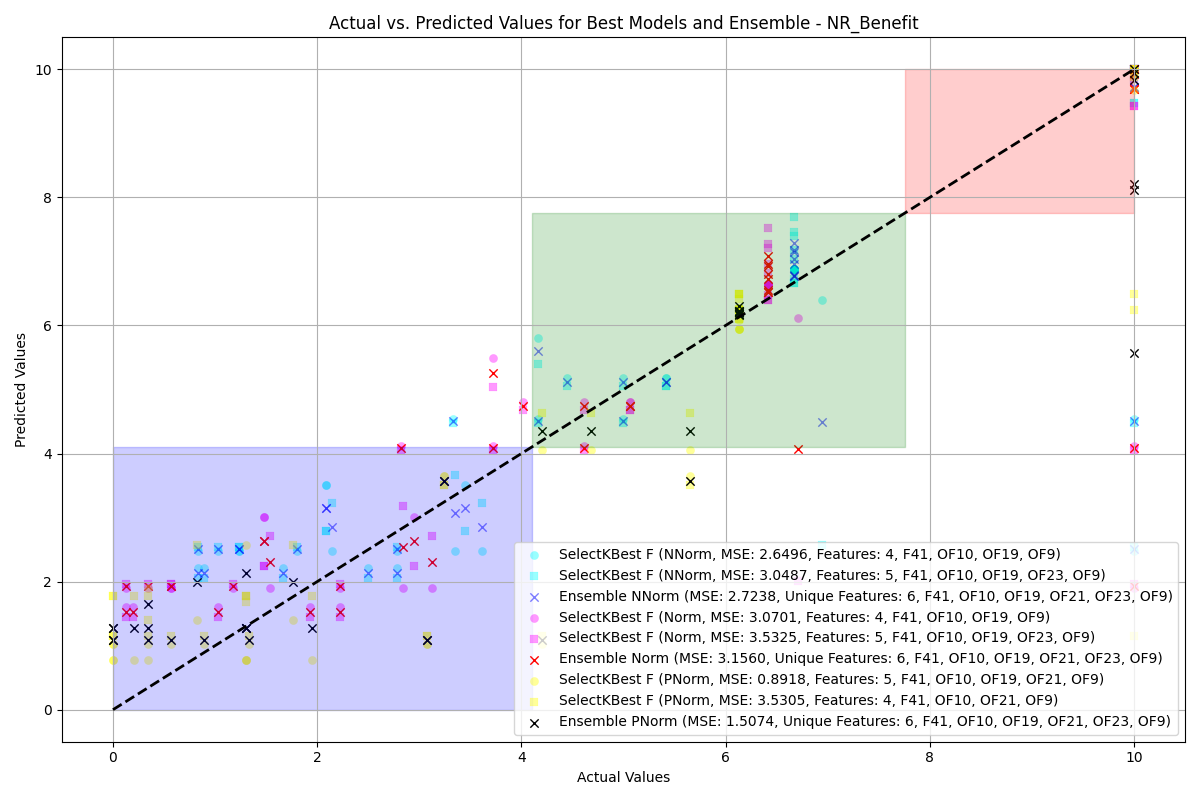
\includegraphics[width=\linewidth]{reg_section_specific/featred_ensemble_learning/actual_vs_predicted_best_feature_selection_and_ensemble_NR_Benefit_10.png}
        \caption{NR Benefit}
        \label{reg_spec_fig:nr_ben_featred}
    \end{minipage}\hfill
    \begin{minipage}{0.45\textwidth}
        \centering
        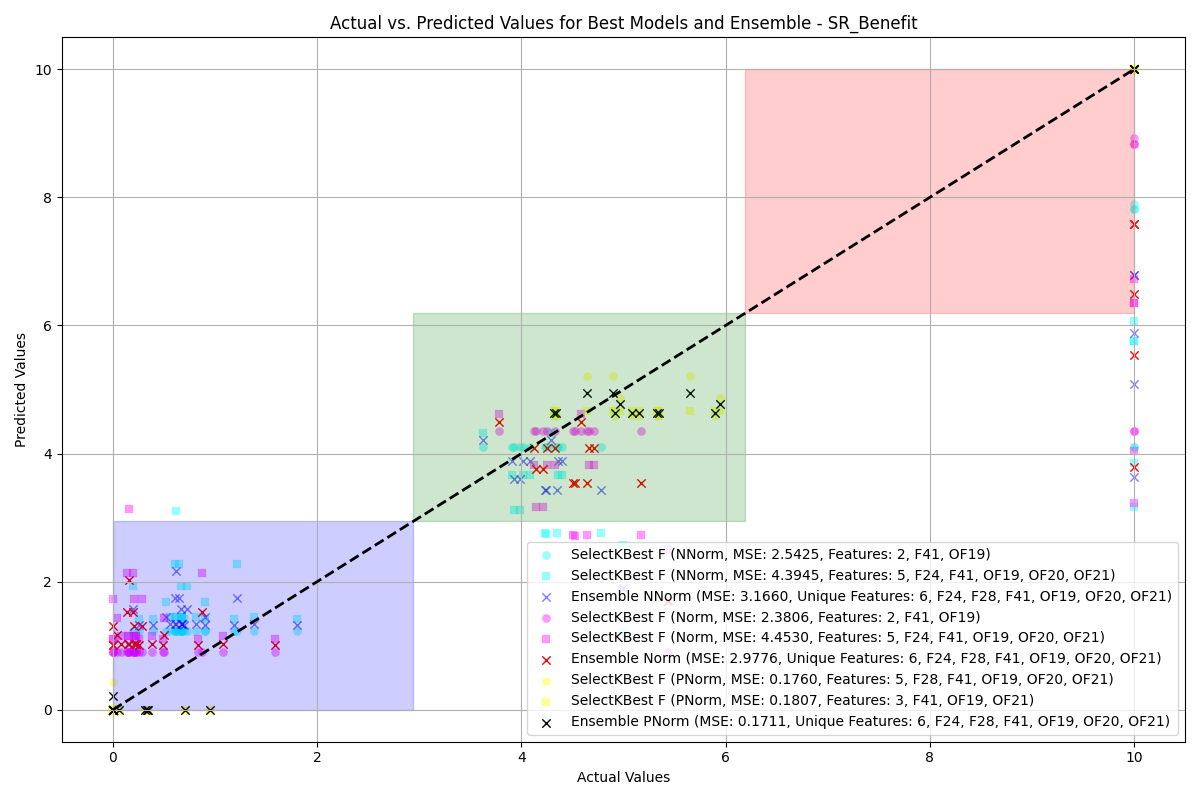
\includegraphics[width=\linewidth]{reg_section_specific/featred_ensemble_learning/actual_vs_predicted_best_feature_selection_and_ensemble_SR_Benefit_10.png}
        \caption{SR Benefit}
        \label{reg_spec_fig:sr_ben_featred}
    \end{minipage}
\end{figure}

\begin{figure}[H]
    \centering
    \begin{minipage}{0.45\textwidth}
        \centering
        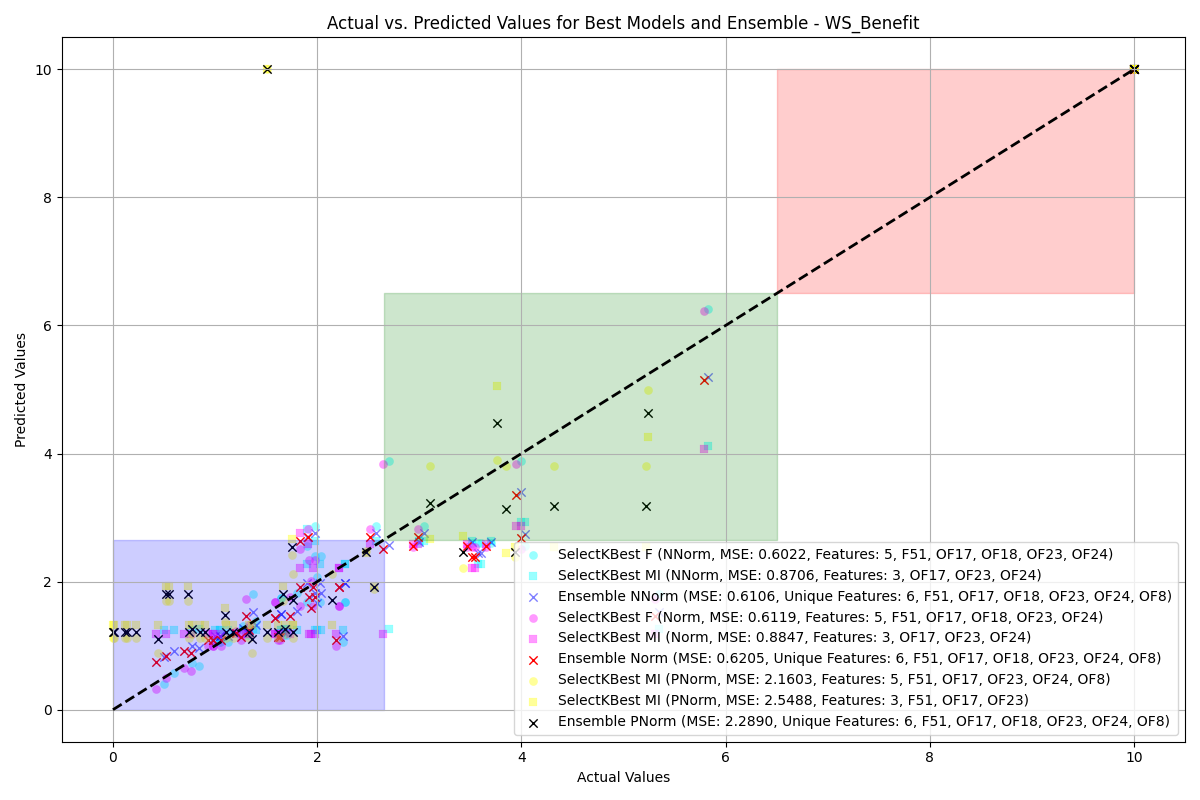
\includegraphics[width=\linewidth]{reg_section_specific/featred_ensemble_learning/actual_vs_predicted_best_feature_selection_and_ensemble_WS_Benefit_10.png}
        \caption{WS Benefit}
        \label{reg_spec_fig:ws_ben_featred}
    \end{minipage}\hfill
    \begin{minipage}{0.45\textwidth}
        \centering
        \includegraphics[width=\linewidth]{reg_section_specific/featred_ensemble_learning/actual_vs_predicted_best_feature_selection_and_ensemble_SFST_Benefit_10.png}
        \caption{SFST Benefit}
        \label{reg_spec_fig:sfst_ben_featred}
    \end{minipage}
\end{figure}

\begin{table}[H]
\centering
\begin{tabular}{|c|c|c|c|c|c|c|}
\hline
\multirow{2}{*}{\textbf{Function}} & \multicolumn{3}{c|}{\textbf{Top Model}} & \multicolumn{3}{c|}{\textbf{Ensemble}} \\
\cline{2-7}
 & \textbf{Lower} & \textbf{Moderate} & \textbf{Higher} & \textbf{Lower} & \textbf{Moderate} & \textbf{Higher} \\
\hline
WS & 100.00\% & 50.00\% & 100.00\% & 100.00\% & 50.00\% & 100.00\% \\
\hline
PR & 0.00\% & 100.00\% & 87.50\% & 0.00\% & 100.00\% & 87.50\% \\
\hline
NR & 57.14\% & 71.43\% & 100.00\% & 28.57\% & 85.71\% & 100.00\% \\
\hline
SR & 90.00\% & 80.00\% & 83.33\% & 90.00\% & 100.00\% & 83.33\% \\
\hline
SFST & 100.00\% & 42.86\% & 100.00\% & 100.00\% & 42.86\% & 100.00\% \\
\hline
WS\_Benefit & 100.00\% & 28.57\% & 100.00\% & 100.00\% & 28.57\% & 100.00\% \\
\hline
PR\_Benefit & 100.00\% & 42.86\% & 50.00\% & 100.00\% & 85.71\% & 50.00\% \\
\hline
NR\_Benefit & 80.00\% & 100.00\% & 75.00\% & 100.00\% & 100.00\% & 75.00\% \\
\hline
SR\_Benefit & 20.00\% & 88.89\% & 0.00\% & 20.00\% & 88.89\% & 0.00\% \\
\hline
SFST\_Benefit & 87.50\% & 50.00\% & 100.00\% & 87.50\% & 50.00\% & 100.00\% \\
\hline
\end{tabular}
\caption{Comparison of Top Model and Ensemble Accuracy for Non-Normalized Data}
\label{reg_all_tab:featred_non_norm_accuracy}
\end{table}

\begin{table}[H]
\centering
\begin{tabular}{|c|c|c|c|c|c|c|}
\hline
\multirow{2}{*}{\textbf{Function}} & \multicolumn{3}{c|}{\textbf{Top Model}} & \multicolumn{3}{c|}{\textbf{Ensemble}} \\
\cline{2-7}
 & \textbf{Lower} & \textbf{Moderate} & \textbf{Higher} & \textbf{Lower} & \textbf{Moderate} & \textbf{Higher} \\
\hline
WS & 100.00\% & 80.00\% & 100.00\% & 100.00\% & 60.00\% & 100.00\% \\
\hline
PR & N/A & 100.00\% & 100.00\% & N/A & 100.00\% & 87.50\% \\
\hline
NR & N/A & 0.00\% & 100.00\% & N/A & 0.00\% & 100.00\% \\
\hline
SR & 0.00\% & 100.00\% & 71.43\% & 0.00\% & 100.00\% & 100.00\% \\
\hline
SFST & 100.00\% & 100.00\% & 0.00\% & 100.00\% & 100.00\% & 0.00\% \\
\hline
WS\_Benefit & 100.00\% & 28.57\% & 100.00\% & 81.82\% & 42.86\% & 100.00\% \\
\hline
PR\_Benefit & 100.00\% & 85.71\% & 50.00\% & 100.00\% & 57.14\% & 50.00\% \\
\hline
NR\_Benefit & 75.00\% & 77.78\% & 75.00\% & 100.00\% & 77.78\% & 75.00\% \\
\hline
SR\_Benefit & 100.00\% & 88.89\% & 0.00\% & 100.00\% & 88.89\% & 0.00\% \\
\hline
SFST\_Benefit & 87.50\% & 100.00\% & 0.00\% & 87.50\% & 100.00\% & 0.00\% \\
\hline
\end{tabular}
\caption{Comparison of Top Model and Ensemble Accuracy for Pre-Normalized Data}
\label{reg_all_tab:featred_norm_accuracy}
\end{table}



\subsubsection{Specific Features}
\begin{table}[H]
\centering
\begin{tabular}{|c|c|c|c|c|}
\hline
\textbf{Feature} & \textbf{NNorm MSE} & \textbf{Norm MSE} & \textbf{Model} & \textbf{Dataset} \\
\hline
NR & 0.17 & 0.48 & AdaBoostRegressor & Interpolated \\
\hline
PR & 0.12 & 0.19 & AdaBoostRegressor & custom \\
\hline
SR & 0.37 & 0.62 & AdaBoostRegressor & bfill \\
\hline
SFST & 0.20 & 0.33 & AdaBoostRegressor & ffill \\
\hline
WS & 0.25 & 0.49 & AdaBoostRegressor & knn \\
\hline
NR Benefit & 0.39 & 0.45 & MLPRegressor & ffill \\
\hline
PR Benefit & 0.22 & 0.23 & SGDRegressor & iterative \\
\hline
SR Benefit & 0.17 & 0.22 & AdaBoostRegressor & bfill \\
\hline
SFST Benefit & 0.51 & 0.98 & AdaBoostRegressor & custom \\
\hline
WS Benefit & 1.19 & 1.21 & AdaBoostRegressor & bfill \\
\hline
\end{tabular}
\caption{Best MSE for Non-Normalized and Normalized Data with Algorithm and Dataset}
\label{reg_all_tab:norm_mse}
\end{table}


\begin{table}[H]
\centering
\begin{tabular}{|c|c|c|c|}
\hline
\textbf{Feature} & \textbf{PNorm MSE} & \textbf{Model} & \textbf{Dataset}  \\
\hline
NR & 0.31& AdaBoostRegressor & knn  \\
\hline
PR  & 0.21 & AdaBoostRegressor & iterative\\
\hline
SR & 0.46 & AdaBoostRegressor & knn \\
\hline
SFST & 0.26& AdaBoostRegressor & custom  \\
\hline
WS & 0.60 & AdaBoostRegressor & custom \\
\hline
NR Benefit & 0.28& MLPRegressor & knn  \\
\hline
PR Benefit  & 0.49 \& MLPRegressor & ffill \\
\hline
SR Benefit & 0.07& SGDRegressor & mode  \\
\hline
SFST Benefit & 0.71& AdaBoostRegressor & iterative  \\
\hline
WS Benefit & 0.63& AdaBoostRegressor & mean  \\
\hline
\end{tabular}
\caption{Best MSE for Pre-Normalized Data}
\label{reg_all_tab:pre_norm_mse}
\end{table}

\begin{figure}[H]
    \centering
    \begin{minipage}{0.45\textwidth}
        \centering
        \includegraphics[width=\linewidth]{reg_section_all/ensemble_learning/actual_vs_predicted_top_3_models_and_ensembles_PR.png}
        \caption{PR}
        \label{reg_all_fig:pr_ensemble}
    \end{minipage}\hfill
    \begin{minipage}{0.45\textwidth}
        \centering
        \includegraphics[width=\linewidth]{reg_section_all/ensemble_learning/actual_vs_predicted_top_3_models_and_ensembles_NR.png}
        \caption{NR}
        \label{reg_all_fig:nr_ensemble}
    \end{minipage}
\end{figure}

\begin{figure}[H]
    \centering
    \begin{minipage}{0.45\textwidth}
        \centering
        \includegraphics[width=\linewidth]{reg_section_all/ensemble_learning/actual_vs_predicted_top_3_models_and_ensembles_SR.png}
        \caption{SR}
        \label{reg_all_fig:sr_ensemble}
    \end{minipage}\hfill
    \begin{minipage}{0.45\textwidth}
        \centering
        \includegraphics[width=\linewidth]{reg_section_all/ensemble_learning/actual_vs_predicted_top_3_models_and_ensembles_WS.png}
        \caption{WS}
        \label{reg_all_fig:ws_ensemble}
    \end{minipage}
\end{figure}

\begin{figure}[H]
    \centering
    \begin{minipage}{0.45\textwidth}
        \centering
        \includegraphics[width=\linewidth]{reg_section_all/ensemble_learning/actual_vs_predicted_top_3_models_and_ensembles_SFST.png}
        \caption{SFST}
        \label{reg_all_fig:sfst_ensemble}
    \end{minipage}\hfill
    \begin{minipage}{0.45\textwidth}
        \centering
        \includegraphics[width=\linewidth]{reg_section_all/ensemble_learning/actual_vs_predicted_top_3_models_and_ensembles_PR_Benefit.png}
        \caption{PR Benefit}
        \label{reg_all_fig:pr_ben_ensemble}
    \end{minipage}
\end{figure}

\begin{figure}[H]
    \centering
    \begin{minipage}{0.45\textwidth}
        \centering
        \includegraphics[width=\linewidth]{reg_section_all/ensemble_learning/actual_vs_predicted_top_3_models_and_ensembles_NR_Benefit.png}
        \caption{NR Benefit}
        \label{reg_all_fig:nr_ben_ensemble}
    \end{minipage}\hfill
    \begin{minipage}{0.45\textwidth}
        \centering
        \includegraphics[width=\linewidth]{reg_section_all/ensemble_learning/actual_vs_predicted_top_3_models_and_ensembles_SR.png}
        \caption{SR Benefit}
        \label{reg_all_fig:sr_ben_ensemble}
    \end{minipage}
\end{figure}

\begin{figure}[H]
    \centering
    \begin{minipage}{0.45\textwidth}
        \centering
        \includegraphics[width=\linewidth]{reg_section_all/ensemble_learning/actual_vs_predicted_top_3_models_and_ensembles_WS_Benefit.png}
        \caption{WS Benefit}
        \label{reg_all_fig:ws_ben_ensemble}
    \end{minipage}\hfill
    \begin{minipage}{0.45\textwidth}
        \centering
        \includegraphics[width=\linewidth]{reg_section_all/ensemble_learning/actual_vs_predicted_top_3_models_and_ensembles_SFST_Benefit.png}
        \caption{SFST Benefit}
        \label{reg_all_fig:sfst_ben_ensemble}
    \end{minipage}
\end{figure}

\begin{longtable}{|p{2cm}|p{2cm}|p{2cm}|p{2cm}|p{2cm}|p{4cm}|}
\hline
\textbf{Model} & \textbf{Lower Acc.} & \textbf{Moderate Acc.} & \textbf{Higher Acc.} & \textbf{Overall Acc.} & \textbf{Top Features} \\ \hline
\endfirsthead
\hline
\textbf{Model} & \textbf{Lower Acc.} & \textbf{Moderate Acc.} & \textbf{Higher Acc.} & \textbf{Overall Acc.} & \textbf{Top Features} \\ \hline
\endhead

WS & 80.81\% & 64.20\% & 70.37\% & 74.07\% & Provincial\_Class, Hydrogeomorphic\_Class, OF22, F22, F28, F31, F43, F44, F45 \\ \hline
PR & 13.89\% & 77.78\% & 87.50\% & 69.31\% & Provincial\_Class, Federal\_Class, F43, F44, F45 \\ \hline
NR & 32.80\% & 65.08\% & 76.19\% & 58.02\% & Provincial\_Class, F24, F43, F44, F45 \\ \hline
SR & 62.22\% & 60.00\% & 62.35\% & 61.73\% & F28, F29, F31, F44, F45 \\ \hline
SFST & 56.17\% & 60.85\% & 76.39\% & 65.43\% & F1, F43 \\ \hline
WS Benefit & 68.35\% & 46.56\% & 44.44\% & 57.67\% & Hydrogeomorphic\_Class, OF17, OF18, OF23, OF24, F51 \\ \hline
PR Benefit & 80.00\% & 44.97\% & 29.63\% & 58.73\% & Regime, Moss\_Cover, Living\_Moss\_Depth, OF19, OF20, OF21, OF22, OF24, F41 \\ \hline
NR Benefit & 70.74\% & 80.42\% & 49.07\% & 69.84\% & Living\_Moss\_Depth, OF9, OF10, OF19, OF20, OF21, OF22, OF23, F41 \\ \hline
SR Benefit & 93.70\% & 53.91\% & 0.00\% & 67.72\% & Provincial\_Class, Federal\_Class, Regime, Vegetation\_Type, Living\_Moss\_Depth, Organic\_Depth, Hydrogeomorphic\_Class, OF18, OF24, F41 \\ \hline
SFST Benefit & 59.72\% & 32.10\% & 48.15\% & 47.97\% & Provincial\_Class, Federal\_Class, Moss\_Cover, Surface\_Water\_Present, Hydrogeomorphic\_Class, OF18, OF22, OF25, OF28 \\ \hline
\caption{Classification Accuracies and Top Features for Various Models}
\label{tab:grouping_1d}
\end{longtable}

\begin{longtable}{|p{1.5cm}|p{2.0cm}|p{2.0cm}|p{2.0cm}|p{2.0cm}|p{4cm}|}
\hline
\textbf{Model} & \textbf{Lower Acc.} & \textbf{Moderate Acc.} & \textbf{Higher Acc.} & \textbf{Overall Acc.} & \textbf{Top Features} \\ \hline
\endfirsthead
\hline
\textbf{Model} & \textbf{Lower Acc.} & \textbf{Moderate Acc.} & \textbf{Higher Acc.} & \textbf{Overall Acc.} & \textbf{Top Features} \\ \hline
\endhead

WS & 100.00\% & 50.00\% & 100.00\% & 85.71\% & F22, F31, F43, F44, F46, F5, OF18, OF27 \\ \hline
PR & 0.00\% & 100.00\% & 100.00\% & 76.19\% & F43, F44, F45, F5, OF18, OF27 \\ \hline
NR & 0.00\% & 71.43\% & 42.86\% & 80.95\% & F43, F44, F45, F5, OF18, OF27, OF34, S4 \\ \hline
SR & 30.00\% & 80.00\% & 50.00\% & 90.48\% & F24, F28, F31, F43, F44, F45, F5, OF18, OF27 \\ \hline
SFST & 100.00\% & 42.86\% & 100.00\% & 80.95\% & F43, F44, F45, F46, OF18, OF27 \\ \hline
WS Benefit & 54.55\% & 71.43\% & 66.67\% & 90.48\% & F5, OF17, OF18, OF23, OF27, OF34, S4 \\ \hline
PR Benefit & 100.00\% & 85.71\% & 25.00\% & 80.95\% & F14, F3\_c, F41, F44, OF18, OF19, OF27 \\ \hline
NR Benefit & 100.00\% & 85.71\% & 50.00\% & 85.71\% & F41, F5, OF10, OF18, OF19, OF22, OF27, OF9 \\ \hline
SR Benefit & 100.00\% & 0.00\% & 0.00\% & 85.71\% & F12, F41, OF18, OF22, OF27, OF30 \\ \hline
SFST Benefit & 37.50\% & 100.00\% & 42.86\% & 80.95\% & F12, F43, F44, F45, F5, OF18, OF27, OF30 \\ \hline
\caption{Ensemble Model Accuracies}
\label{tab:grouping_2d}
\end{longtable}

\begin{longtable}{|p{1.5cm}|p{2.0cm}|p{2.0cm}|p{2.0cm}|p{2.0cm}|p{4cm}|}
\hline
\textbf{Model} & \textbf{Lower Acc.} & \textbf{Moderate Acc.} & \textbf{Higher Acc.} & \textbf{Overall Acc.} & \textbf{Top Features} \\ \hline
\endfirsthead
\hline
\textbf{Model} & \textbf{Lower Acc.} & \textbf{Moderate Acc.} & \textbf{Higher Acc.} & \textbf{Overall Acc.} & \textbf{Top Features} \\ \hline
\endhead

WS & 100.00\% & 50.00\% & 75.00\% & 85.71\% & F22, F31, F43, F44, F46, F5, OF18, OF27 \\ \hline
PR & 0.00\% & 100.00\% & 100.00\% & 76.19\% & F43, F44, F45, F5, OF18, OF27 \\ \hline
NR & 0.00\% & 85.71\% & 42.86\% & 61.90\% & F43, F44, F45, F5, OF18, OF27, OF34, S4 \\ \hline
SR & 30.00\% & 80.00\% & 33.33\% & 85.71\% & F24, F28, F31, F43, F44, F45, F5, OF18, OF27 \\ \hline
SFST & 100.00\% & 42.86\% & 100.00\% & 80.95\% & F43, F44, F45, F46, OF18, OF27 \\ \hline
WS Benefit & 36.36\% & 71.43\% & 66.67\% & 80.95\% & F5, OF17, OF18, OF23, OF27, OF34, S4 \\ \hline
PR Benefit & 100.00\% & 85.71\% & 25.00\% & 80.95\% & F14, F3\_c, F41, F44, OF18, OF19, OF27 \\ \hline
NR Benefit & 100.00\% & 85.71\% & 50.00\% & 76.19\% & F41, F5, OF10, OF18, OF19, OF22, OF27, OF9 \\ \hline
SR Benefit & 100.00\% & 0.00\% & 0.00\% & 47.62\% & F12, F41, OF18, OF22, OF27, OF30 \\ \hline
SFST Benefit & 37.50\% & 100.00\% & 42.86\% & 57.14\% & F12, F43, F44, F45, F5, OF18, OF27, OF30 \\ \hline

\caption{Voting System Accuracies}
\label{tab:grouping_3d}
\end{longtable}

\begin{figure}[H]
    \centering
    \begin{minipage}{0.45\textwidth}
        \centering
        \includegraphics[width=\linewidth]{reg_section_specific/featred_ensemble_learning/actual_vs_predicted_best_feature_selection_and_ensemble_PR_10.png}
        \caption{PR}
        \label{reg_spec_fig:pr_featred}
    \end{minipage}\hfill
    \begin{minipage}{0.45\textwidth}
        \centering
        \includegraphics[width=\linewidth]{reg_section_specific/featred_ensemble_learning/actual_vs_predicted_best_feature_selection_and_ensemble_NR_10.png}
        \caption{NR}
        \label{reg_spec_fig:nr_featred}
    \end{minipage}
\end{figure}

\begin{figure}[H]
    \centering
    \begin{minipage}{0.45\textwidth}
        \centering
        \includegraphics[width=\linewidth]{reg_section_specific/featred_ensemble_learning/actual_vs_predicted_best_feature_selection_and_ensemble_SR_10.png}
        \caption{SR}
        \label{reg_spec_fig:sr_featred}
    \end{minipage}\hfill
    \begin{minipage}{0.45\textwidth}
        \centering
        \includegraphics[width=\linewidth]{reg_section_specific/featred_ensemble_learning/actual_vs_predicted_best_feature_selection_and_ensemble_WS_10.png}
        \caption{WS}
        \label{reg_spec_fig:ws_featred}
    \end{minipage}
\end{figure}

\begin{figure}[H]
    \centering
    \begin{minipage}{0.45\textwidth}
        \centering
        \includegraphics[width=\linewidth]{reg_section_specific/featred_ensemble_learning/actual_vs_predicted_best_feature_selection_and_ensemble_SFST_10.png}
        \caption{SFST}
        \label{reg_spec_fig:sfst_featred}
    \end{minipage}\hfill
    \begin{minipage}{0.45\textwidth}
        \centering
        \includegraphics[width=\linewidth]{reg_section_specific/featred_ensemble_learning/actual_vs_predicted_best_feature_selection_and_ensemble_PR_Benefit_10.png}
        \caption{PR Benefit}
        \label{reg_spec_fig:pr_ben_featred}
    \end{minipage}
\end{figure}

\begin{figure}[H]
    \centering
    \begin{minipage}{0.45\textwidth}
        \centering
        \includegraphics[width=\linewidth]{reg_section_specific/featred_ensemble_learning/actual_vs_predicted_best_feature_selection_and_ensemble_NR_Benefit_10.png}
        \caption{NR Benefit}
        \label{reg_spec_fig:nr_ben_featred}
    \end{minipage}\hfill
    \begin{minipage}{0.45\textwidth}
        \centering
        \includegraphics[width=\linewidth]{reg_section_specific/featred_ensemble_learning/actual_vs_predicted_best_feature_selection_and_ensemble_SR_Benefit_10.png}
        \caption{SR Benefit}
        \label{reg_spec_fig:sr_ben_featred}
    \end{minipage}
\end{figure}

\begin{figure}[H]
    \centering
    \begin{minipage}{0.45\textwidth}
        \centering
        \includegraphics[width=\linewidth]{reg_section_specific/featred_ensemble_learning/actual_vs_predicted_best_feature_selection_and_ensemble_WS_Benefit_10.png}
        \caption{WS Benefit}
        \label{reg_spec_fig:ws_ben_featred}
    \end{minipage}\hfill
    \begin{minipage}{0.45\textwidth}
        \centering
        \includegraphics[width=\linewidth]{reg_section_specific/featred_ensemble_learning/actual_vs_predicted_best_feature_selection_and_ensemble_SFST_Benefit_10.png}
        \caption{SFST Benefit}
        \label{reg_spec_fig:sfst_ben_featred}
    \end{minipage}
\end{figure}

\begin{table}[H]
\centering
\begin{tabular}{|c|c|c|c|c|c|c|}
\hline
\multirow{2}{*}{\textbf{Function}} & \multicolumn{3}{c|}{\textbf{Top Model}} & \multicolumn{3}{c|}{\textbf{Ensemble}} \\
\cline{2-7}
 & \textbf{Lower} & \textbf{Moderate} & \textbf{Higher} & \textbf{Lower} & \textbf{Moderate} & \textbf{Higher} \\
\hline
WS & 100.00\% & 50.00\% & 100.00\% & 100.00\% & 50.00\% & 100.00\% \\
\hline
PR & 0.00\% & 100.00\% & 87.50\% & 0.00\% & 100.00\% & 87.50\% \\
\hline
NR & 57.14\% & 71.43\% & 100.00\% & 28.57\% & 85.71\% & 100.00\% \\
\hline
SR & 90.00\% & 80.00\% & 83.33\% & 90.00\% & 100.00\% & 83.33\% \\
\hline
SFST & 100.00\% & 42.86\% & 100.00\% & 100.00\% & 42.86\% & 100.00\% \\
\hline
WS\_Benefit & 100.00\% & 28.57\% & 100.00\% & 100.00\% & 28.57\% & 100.00\% \\
\hline
PR\_Benefit & 100.00\% & 42.86\% & 50.00\% & 100.00\% & 85.71\% & 50.00\% \\
\hline
NR\_Benefit & 80.00\% & 100.00\% & 75.00\% & 100.00\% & 100.00\% & 75.00\% \\
\hline
SR\_Benefit & 20.00\% & 88.89\% & 0.00\% & 20.00\% & 88.89\% & 0.00\% \\
\hline
SFST\_Benefit & 87.50\% & 50.00\% & 100.00\% & 87.50\% & 50.00\% & 100.00\% \\
\hline
\end{tabular}
\caption{Comparison of Top Model and Ensemble Accuracy for Non-Normalized Data}
\label{reg_all_tab:featred_non_norm_accuracy}
\end{table}

\begin{table}[H]
\centering
\begin{tabular}{|c|c|c|c|c|c|c|}
\hline
\multirow{2}{*}{\textbf{Function}} & \multicolumn{3}{c|}{\textbf{Top Model}} & \multicolumn{3}{c|}{\textbf{Ensemble}} \\
\cline{2-7}
 & \textbf{Lower} & \textbf{Moderate} & \textbf{Higher} & \textbf{Lower} & \textbf{Moderate} & \textbf{Higher} \\
\hline
WS & 100.00\% & 80.00\% & 100.00\% & 100.00\% & 60.00\% & 100.00\% \\
\hline
PR & N/A & 100.00\% & 100.00\% & N/A & 100.00\% & 87.50\% \\
\hline
NR & N/A & 0.00\% & 100.00\% & N/A & 0.00\% & 100.00\% \\
\hline
SR & 0.00\% & 100.00\% & 71.43\% & 0.00\% & 100.00\% & 100.00\% \\
\hline
SFST & 100.00\% & 100.00\% & 0.00\% & 100.00\% & 100.00\% & 0.00\% \\
\hline
WS\_Benefit & 100.00\% & 28.57\% & 100.00\% & 81.82\% & 42.86\% & 100.00\% \\
\hline
PR\_Benefit & 100.00\% & 85.71\% & 50.00\% & 100.00\% & 57.14\% & 50.00\% \\
\hline
NR\_Benefit & 75.00\% & 77.78\% & 75.00\% & 100.00\% & 77.78\% & 75.00\% \\
\hline
SR\_Benefit & 100.00\% & 88.89\% & 0.00\% & 100.00\% & 88.89\% & 0.00\% \\
\hline
SFST\_Benefit & 87.50\% & 100.00\% & 0.00\% & 87.50\% & 100.00\% & 0.00\% \\
\hline
\end{tabular}
\caption{Comparison of Top Model and Ensemble Accuracy for Pre-Normalized Data}
\label{reg_all_tab:featred_norm_accuracy}
\end{table}




\subsection{CausalML}

\begin{figure}
    \centering
    \includegraphics[width=0.95\linewidth]{./causalml_section/graphs/feature_importance_points_plot_PR.png}
    \caption{PR}
    \label{fig:pr_causalml}
\end{figure}

\begin{figure}
    \centering
    \includegraphics[width=0.95\linewidth]{./causalml_section/graphs/feature_importance_points_plot_NR.png}
    \caption{NR}
    \label{fig:nr_causalml}
\end{figure}

\begin{figure}
    \centering
    \includegraphics[width=0.95\linewidth]{./causalml_section/graphs/feature_importance_points_plot_SR.png}
    \caption{SR}
    \label{fig:sr_causalml}
\end{figure}

\begin{figure}
    \centering
    \includegraphics[width=0.95\linewidth]{./causalml_section/graphs/feature_importance_points_plot_WS.png}
    \caption{WS}
    \label{fig:ws_causalml}
\end{figure}

\begin{figure}
    \centering
    \includegraphics[width=0.95\linewidth]{./causalml_section/graphs/feature_importance_points_plot_SFST.png}
    \caption{SFST}
    \label{fig:sfst_causalml}
\end{figure}



\begin{figure}
    \centering
    \includegraphics[width=0.95\linewidth]{./causalml_section/graphs/feature_importance_points_plot_PR_Benefit.png}
    \caption{PR Benefit}
    \label{fig:pr_ben_causalml}
\end{figure}

\begin{figure}
    \centering
    \includegraphics[width=0.95\linewidth]{./causalml_section/graphs/feature_importance_points_plot_NR_Benefit.png}
    \caption{NR Benefit}
    \label{fig:nr_ben_causalml}
\end{figure}

\begin{figure}
    \centering
    \includegraphics[width=0.95\linewidth]{./causalml_section/graphs/feature_importance_points_plot_SR_Benefit.png}
    \caption{SR Benefit}
    \label{fig:sr_ben_causalml}
\end{figure}

\begin{figure}
    \centering
    \includegraphics[width=0.95\linewidth]{./causalml_section/graphs/feature_importance_points_plot_WS_Benefit.png}
    \caption{WS Benefit}
    \label{fig:ws_ben_causalml}
\end{figure}

\begin{figure}
    \centering
    \includegraphics[width=0.95\linewidth]{./causalml_section/graphs/feature_importance_points_plot_SFST_Benefit.png}
    \caption{SFST Benefit}
    \label{fig:sfst_ben_causalml}
\end{figure}



\begin{table}
\centering
\begin{tabular}{|l|l|l|}
\hline
\textbf{Model} & \textbf{Top 2 Important Features} & \textbf{Bottom 2 Important Features} \\
\hline
Ridge & 
\begin{tabular}[c]{@{}l@{}}
'F43': 0.536779\\
'F45': 0.192897\\
\end{tabular} & 
\begin{tabular}[c]{@{}l@{}}
'OF8': -0.012789\\
'OF13': -0.009090\\
\end{tabular} \\
\hline
DecisionTreeRegressor & 
\begin{tabular}[c]{@{}l@{}}
'F43': 1.515596\\
'F29': 0.037213\\
\end{tabular} & 
\begin{tabular}[c]{@{}l@{}}
'F65': -0.022642\\
'F24': -0.017126\\
\end{tabular} \\
\hline
GradientBoostingRegressor & 
\begin{tabular}[c]{@{}l@{}}
'F43': 1.346256\\
'OF26': 0.021221\\
\end{tabular} & 
\begin{tabular}[c]{@{}l@{}}
'F3d': -0.003275\\
'F13': -0.000601\\
\end{tabular} \\
\hline
RandomForestRegressor & 
\begin{tabular}[c]{@{}l@{}}
'F43': 1.182576\\
'OF26': 0.042053\\
\end{tabular} & 
\begin{tabular}[c]{@{}l@{}}
'F13': -0.001210\\
'F3f': -0.000922\\
\end{tabular} \\
\hline
AdaBoostRegressor & 
\begin{tabular}[c]{@{}l@{}}
'F43': 1.431664\\
'OF26': 0.020958\\
\end{tabular} & 
\begin{tabular}[c]{@{}l@{}}
'F15': -0.001777\\
'F49': -0.001246\\
\end{tabular} \\
\hline
KNeighborsRegressor & 
\begin{tabular}[c]{@{}l@{}}
'F5': 0.708910\\
'F3d': 0.003255\\
\end{tabular} & 
\begin{tabular}[c]{@{}l@{}}
'OF27': -0.055648\\
'F41': 0.000000\\
\end{tabular} \\
\hline
MLPRegressor & 
\begin{tabular}[c]{@{}l@{}}
'OF27': 1.309096\\
'F14': 0.515494\\
\end{tabular} & 
\begin{tabular}[c]{@{}l@{}}
'F5': -2.923432\\
'F25': -0.309051\\
\end{tabular} \\
\hline
ElasticNet & 
\begin{tabular}[c]{@{}l@{}}
'F43': 0.441983\\
'F45': 0.245119\\
\end{tabular} & 
\begin{tabular}[c]{@{}l@{}}
'OF2': 0.000000\\
'F39': 0.000000\\
\end{tabular} \\
\hline
SVR & 
\begin{tabular}[c]{@{}l@{}}
'F5': 0.048764\\
'OF27': 0.010900\\
\end{tabular} & 
\begin{tabular}[c]{@{}l@{}}
'OF18': -0.000016\\
'F3g': -0.000009\\
\end{tabular} \\
\hline
BayesianRidge & 
\begin{tabular}[c]{@{}l@{}}
'F43': 0.383303\\
'F45': 0.171036\\
\end{tabular} & 
\begin{tabular}[c]{@{}l@{}}
'OF8': -0.004480\\
'OF38': -0.003056\\
\end{tabular} \\
\hline
KernelRidge & 
\begin{tabular}[c]{@{}l@{}}
'F43': 0.542174\\
'F45': 0.191382\\
\end{tabular} & 
\begin{tabular}[c]{@{}l@{}}
'OF8': -0.013750\\
'OF13': -0.008700\\
\end{tabular} \\
\hline
LinearRegression & 
\begin{tabular}[c]{@{}l@{}}
'F43': 0.590500\\
'F7': 0.202867\\
\end{tabular} & 
\begin{tabular}[c]{@{}l@{}}
'OF8': -0.012748\\
'OF6': -0.011382\\
\end{tabular} \\
\hline
RANSACRegressor & 
\begin{tabular}[c]{@{}l@{}}
'OF21': 9.560983\\
'OF20': 7.545941\\
\end{tabular} & 
\begin{tabular}[c]{@{}l@{}}
'F52': -0.194904\\
'OF16': -0.166460\\
\end{tabular} \\
\hline
TheilSenRegressor & 
\begin{tabular}[c]{@{}l@{}}
'F43': 0.393848\\
'F45': 0.244852\\
\end{tabular} & 
\begin{tabular}[c]{@{}l@{}}
'OF28': -0.006563\\
'OF8': -0.006284\\
\end{tabular} \\
\hline
\textbf{Average Importance} & \begin{tabular}[c]{@{}l@{}}'Feature OF21': 0.702052\\
'Feature F43': 0.625989\\
'Feature OF20': 0.544127\\
'Feature F45': 0.135707\\
\end{tabular} & \begin{tabular}[c]{@{}l@{}}'Feature F25': -0.009865\\
'Feature OF16': -0.011711\\
'Feature OF6': -0.011840\\
'Feature F5': -0.138349\\
\end{tabular} \\ \hline\textbf{Voting System} & \begin{tabular}[c]{@{}l@{}}'Feature F43': 1321 points\\
'Feature F1': 1186 points\\
'Feature F14': 1171 points\\
'Feature F7': 1150 points\\
\end{tabular} & \begin{tabular}[c]{@{}l@{}}'Feature OF28': 421 points\\
'Feature OF13': 408 points\\
'Feature F39': 381 points\\
'Feature OF2': 377 points\\
\end{tabular} \\ \hline
\end{tabular}
\caption{Features for PR Models}
\label{tab:important_features_PR}
\end{table}






\begin{table}[h!]
\centering
\begin{tabular}{|l|l|l|}
\hline
\textbf{Model} & \textbf{Top 2 Important Features} & \textbf{Bottom 2 Important Features} \\
\hline
Ridge & 
\begin{tabular}[c]{@{}l@{}}
'F43': 0.390725\\
'F44': 0.165844\\
\end{tabular} & 
\begin{tabular}[c]{@{}l@{}}
'OF6': -0.020725\\
'OF33': -0.013250\\
\end{tabular} \\
\hline
DecisionTreeRegressor & 
\begin{tabular}[c]{@{}l@{}}
'F43': 1.774561\\
'F24': 0.057620\\
\end{tabular} & 
\begin{tabular}[c]{@{}l@{}}
'F3e': -0.008175\\
'F49': -0.005408\\
\end{tabular} \\
\hline
GradientBoostingRegressor & 
\begin{tabular}[c]{@{}l@{}}
'F43': 1.620630\\
'F24': 0.022750\\
\end{tabular} & 
\begin{tabular}[c]{@{}l@{}}
'F3c': -0.000362\\
'F12': -0.000226\\
\end{tabular} \\
\hline
RandomForestRegressor & 
\begin{tabular}[c]{@{}l@{}}
'F43': 0.817959\\
'F12': 0.218402\\
\end{tabular} & 
\begin{tabular}[c]{@{}l@{}}
'F47': -0.011895\\
'F21': -0.009079\\
\end{tabular} \\
\hline
AdaBoostRegressor & 
\begin{tabular}[c]{@{}l@{}}
'F43': 1.720332\\
'F24': 0.038324\\
\end{tabular} & 
\begin{tabular}[c]{@{}l@{}}
'F50': -0.000827\\
'F12': -0.000806\\
\end{tabular} \\
\hline
KNeighborsRegressor & 
\begin{tabular}[c]{@{}l@{}}
'F5': 0.533441\\
'OF27': 0.061891\\
\end{tabular} & 
\begin{tabular}[c]{@{}l@{}}
'OF13': -0.000245\\
'OF9': -0.000204\\
\end{tabular} \\
\hline
MLPRegressor & 
\begin{tabular}[c]{@{}l@{}}
'F5': 0.153295\\
'F45': 0.111910\\
\end{tabular} & 
\begin{tabular}[c]{@{}l@{}}
'F2': -0.017481\\
'F14': -0.014245\\
\end{tabular} \\
\hline
ElasticNet & 
\begin{tabular}[c]{@{}l@{}}
'F43': 0.506674\\
'F45': 0.266837\\
\end{tabular} & 
\begin{tabular}[c]{@{}l@{}}
'OF2': 0.000000\\
'F38': 0.000000\\
\end{tabular} \\
\hline
SVR & 
\begin{tabular}[c]{@{}l@{}}
'F5': 0.025143\\
'OF27': 0.006574\\
\end{tabular} & 
\begin{tabular}[c]{@{}l@{}}
'OF5': -0.000005\\
'F3g': -0.000004\\
\end{tabular} \\
\hline
BayesianRidge & 
\begin{tabular}[c]{@{}l@{}}
'F43': 0.428843\\
'F45': 0.148416\\
\end{tabular} & 
\begin{tabular}[c]{@{}l@{}}
'OF6': -0.007226\\
'OF34': -0.006675\\
\end{tabular} \\
\hline
KernelRidge & 
\begin{tabular}[c]{@{}l@{}}
'F43': 0.406266\\
'F44': 0.176189\\
\end{tabular} & 
\begin{tabular}[c]{@{}l@{}}
'OF6': -0.021310\\
'OF8': -0.014864\\
\end{tabular} \\
\hline
LinearRegression & 
\begin{tabular}[c]{@{}l@{}}
'F43': 0.346340\\
'F44': 0.199381\\
\end{tabular} & 
\begin{tabular}[c]{@{}l@{}}
'OF6': -0.027631\\
'OF33': -0.018511\\
\end{tabular} \\
\hline
RANSACRegressor & 
\begin{tabular}[c]{@{}l@{}}
'F45': 0.448435\\
'F44': 0.221599\\
\end{tabular} & 
\begin{tabular}[c]{@{}l@{}}
'F33': -0.038320\\
'F8': -0.023706\\
\end{tabular} \\
\hline
TheilSenRegressor & 
\begin{tabular}[c]{@{}l@{}}
'F43': 0.316211\\
'F44': 0.201227\\
\end{tabular} & 
\begin{tabular}[c]{@{}l@{}}
'OF6': -0.027462\\
'OF33': -0.015219\\
\end{tabular} \\
\hline
\textbf{Average Importance} & \begin{tabular}[c]{@{}l@{}}'Feature F43': 0.612435\\
'Feature F45': 0.117268\\
'Feature F44': 0.081121\\
'Feature F5': 0.053705\\
\end{tabular} & \begin{tabular}[c]{@{}l@{}}'Feature F8': -0.004219\\
'Feature F33': -0.004765\\
'Feature OF6': -0.005082\\
'Feature OF33': -0.006181\\
\end{tabular} \\ \hline\textbf{Voting System} & \begin{tabular}[c]{@{}l@{}}'Feature F43': 1343 points\\
'Feature F45': 1220 points\\
'Feature F44': 1151 points\\
'Feature F3f': 1137 points\\
\end{tabular} & \begin{tabular}[c]{@{}l@{}}'Feature F32': 377 points\\
'Feature F67': 360 points\\
'Feature F33': 358 points\\
'Feature F39': 352 points\\
\end{tabular} \\ \hline
\end{tabular}
\caption{Features for NR Models}
\label{tab:important_features_NR}
\end{table}
\begin{table}[h!]
\centering
\begin{tabular}{|l|l|l|}
\hline
\textbf{Model} & \textbf{Top 2 Important Features} & \textbf{Bottom 2 Important Features} \\
\hline
Ridge & 
\begin{tabular}[c]{@{}l@{}}
'F43': 1.147478\\
'F45': 0.091115\\
\end{tabular} & 
\begin{tabular}[c]{@{}l@{}}
'OF24': -0.025517\\
'F24': -0.016204\\
\end{tabular} \\
\hline
DecisionTreeRegressor & 
\begin{tabular}[c]{@{}l@{}}
'F43': 1.754513\\
'F22': 0.147253\\
\end{tabular} & 
\begin{tabular}[c]{@{}l@{}}
'F20': -0.014787\\
'F29': -0.009592\\
\end{tabular} \\
\hline
GradientBoostingRegressor & 
\begin{tabular}[c]{@{}l@{}}
'F43': 1.511286\\
'F22': 0.110634\\
\end{tabular} & 
\begin{tabular}[c]{@{}l@{}}
'F20': -0.003293\\
'F46': -0.001353\\
\end{tabular} \\
\hline
RandomForestRegressor & 
\begin{tabular}[c]{@{}l@{}}
'F43': 1.575029\\
'F22': 0.124296\\
\end{tabular} & 
\begin{tabular}[c]{@{}l@{}}
'F20': -0.006019\\
'F2': -0.002894\\
\end{tabular} \\
\hline
AdaBoostRegressor & 
\begin{tabular}[c]{@{}l@{}}
'F43': 1.391152\\
'F22': 0.044818\\
\end{tabular} & 
\begin{tabular}[c]{@{}l@{}}
'OF6': -0.003275\\
'F51': -0.002221\\
\end{tabular} \\
\hline
KNeighborsRegressor & 
\begin{tabular}[c]{@{}l@{}}
'F5': 0.559163\\
'OF27': 0.011390\\
\end{tabular} & 
\begin{tabular}[c]{@{}l@{}}
'OF13': -0.001688\\
'OF9': -0.001394\\
\end{tabular} \\
\hline
MLPRegressor & 
\begin{tabular}[c]{@{}l@{}}
'F5': 0.805548\\
'OF27': 0.188689\\
\end{tabular} & 
\begin{tabular}[c]{@{}l@{}}
'F45': -0.084892\\
'F3e': -0.080038\\
\end{tabular} \\
\hline
ElasticNet & 
\begin{tabular}[c]{@{}l@{}}
'F43': 0.898375\\
'F25': 0.020736\\
\end{tabular} & 
\begin{tabular}[c]{@{}l@{}}
'OF27': -0.003515\\
'OF18': -0.000012\\
\end{tabular} \\
\hline
SVR & 
\begin{tabular}[c]{@{}l@{}}
'F5': 0.036869\\
'F43': 0.000169\\
\end{tabular} & 
\begin{tabular}[c]{@{}l@{}}
'OF27': -0.001506\\
'OF18': -0.000024\\
\end{tabular} \\
\hline
BayesianRidge & 
\begin{tabular}[c]{@{}l@{}}
'F43': 0.726329\\
'F3b': 0.036111\\
\end{tabular} & 
\begin{tabular}[c]{@{}l@{}}
'F68': -0.006553\\
'F6': -0.005987\\
\end{tabular} \\
\hline
KernelRidge & 
\begin{tabular}[c]{@{}l@{}}
'F43': 1.163232\\
'F52': 0.098785\\
\end{tabular} & 
\begin{tabular}[c]{@{}l@{}}
'OF24': -0.025737\\
'F24': -0.017471\\
\end{tabular} \\
\hline
LinearRegression & 
\begin{tabular}[c]{@{}l@{}}
'F43': 1.185014\\
'F52': 0.186445\\
\end{tabular} & 
\begin{tabular}[c]{@{}l@{}}
'OF24': -0.041529\\
'F24': -0.022150\\
\end{tabular} \\
\hline
RANSACRegressor & 
\begin{tabular}[c]{@{}l@{}}
'F43': 0.787310\\
'F22': 0.434157\\
\end{tabular} & 
\begin{tabular}[c]{@{}l@{}}
'F12': -0.331444\\
'F18': -0.283120\\
\end{tabular} \\
\hline
TheilSenRegressor & 
\begin{tabular}[c]{@{}l@{}}
'F43': 1.195570\\
'F52': 0.204452\\
\end{tabular} & 
\begin{tabular}[c]{@{}l@{}}
'OF24': -0.036281\\
'OF21': -0.026817\\
\end{tabular} \\
\hline
\textbf{Average Importance} & \begin{tabular}[c]{@{}l@{}}'Feature F43': 0.951765\\
'Feature F5': 0.097695\\
'Feature F22': 0.091916\\
'Feature F52': 0.048698\\
\end{tabular} & \begin{tabular}[c]{@{}l@{}}'Feature OF20': -0.008094\\
'Feature F62': -0.009468\\
'Feature F18': -0.020177\\
'Feature F12': -0.026529\\
\end{tabular} \\ \hline\textbf{Voting System} & \begin{tabular}[c]{@{}l@{}}'Feature F43': 1346 points\\
'Feature F22': 1265 points\\
'Feature OF22': 1214 points\\
'Feature F25': 1178 points\\
\end{tabular} & \begin{tabular}[c]{@{}l@{}}'Feature F68': 451 points\\
'Feature F18': 439 points\\
'Feature OF8': 398 points\\
'Feature F62': 387 points\\
\end{tabular} \\ \hline
\end{tabular}
\caption{Features for WS Models}
\label{tab:important_features_WS}
\end{table}

\begin{table}[h!]
\centering
\begin{tabular}{|l|l|l|}
\hline
\textbf{Model} & \textbf{Top 2 Important Features} & \textbf{Bottom 2 Important Features} \\
\hline
Ridge & 
\begin{tabular}[c]{@{}l@{}}
'F43': 1.145591\\
'F1': 0.032092\\
\end{tabular} & 
\begin{tabular}[c]{@{}l@{}}
'F49': -0.007396\\
'F15': -0.004882\\
\end{tabular} \\
\hline
DecisionTreeRegressor & 
\begin{tabular}[c]{@{}l@{}}
'F43': 1.956398\\
'F48': 0.016230\\
\end{tabular} & 
\begin{tabular}[c]{@{}l@{}}
'OF3': -0.012433\\
'F47': -0.006130\\
\end{tabular} \\
\hline
GradientBoostingRegressor & 
\begin{tabular}[c]{@{}l@{}}
'F43': 1.658540\\
'F21': 0.016892\\
\end{tabular} & 
\begin{tabular}[c]{@{}l@{}}
'OF18': -0.003418\\
'F2': -0.001442\\
\end{tabular} \\
\hline
RandomForestRegressor & 
\begin{tabular}[c]{@{}l@{}}
'F43': 1.507879\\
'F44': 0.017893\\
\end{tabular} & 
\begin{tabular}[c]{@{}l@{}}
'F65': -0.002316\\
'OF15': -0.001130\\
\end{tabular} \\
\hline
AdaBoostRegressor & 
\begin{tabular}[c]{@{}l@{}}
'F43': 1.680548\\
'F21': 0.008374\\
\end{tabular} & 
\begin{tabular}[c]{@{}l@{}}
'OF18': -0.005203\\
'F8': -0.003271\\
\end{tabular} \\
\hline
KNeighborsRegressor & 
\begin{tabular}[c]{@{}l@{}}
'F5': 0.650557\\
'OF27': 0.009803\\
\end{tabular} & 
\begin{tabular}[c]{@{}l@{}}
'OF13': -0.001657\\
'OF9': -0.001100\\
\end{tabular} \\
\hline
MLPRegressor & 
\begin{tabular}[c]{@{}l@{}}
'F5': 6.260377\\
'OF27': 1.699317\\
\end{tabular} & 
\begin{tabular}[c]{@{}l@{}}
'F35': -0.410244\\
'F36': -0.313736\\
\end{tabular} \\
\hline
ElasticNet & 
\begin{tabular}[c]{@{}l@{}}
'F43': 0.809538\\
'F45': 0.102403\\
\end{tabular} & 
\begin{tabular}[c]{@{}l@{}}
'OF18': -0.000019\\
'OF2': 0.000000\\
\end{tabular} \\
\hline
SVR & 
\begin{tabular}[c]{@{}l@{}}
'F5': 0.026701\\
'F43': 0.000142\\
\end{tabular} & 
\begin{tabular}[c]{@{}l@{}}
'OF18': -0.000016\\
'OF5': -0.000004\\
\end{tabular} \\
\hline
BayesianRidge & 
\begin{tabular}[c]{@{}l@{}}
'F43': 0.811364\\
'F34': 0.018542\\
\end{tabular} & 
\begin{tabular}[c]{@{}l@{}}
'F15': -0.002554\\
'OF8': -0.002456\\
\end{tabular} \\
\hline
KernelRidge & 
\begin{tabular}[c]{@{}l@{}}
'F43': 1.142568\\
'F1': 0.031358\\
\end{tabular} & 
\begin{tabular}[c]{@{}l@{}}
'F49': -0.007572\\
'F15': -0.004914\\
\end{tabular} \\
\hline
LinearRegression & 
\begin{tabular}[c]{@{}l@{}}
'F43': 1.219160\\
'F1': 0.046488\\
\end{tabular} & 
\begin{tabular}[c]{@{}l@{}}
'F49': -0.009860\\
'F31': -0.005465\\
\end{tabular} \\
\hline
RANSACRegressor & 
\begin{tabular}[c]{@{}l@{}}
'F43': 1.518405\\
'F34': 0.129466\\
\end{tabular} & 
\begin{tabular}[c]{@{}l@{}}
'F36': -0.016735\\
'F48': -0.012570\\
\end{tabular} \\
\hline
TheilSenRegressor & 
\begin{tabular}[c]{@{}l@{}}
'F43': 1.308138\\
'F1': 0.044073\\
\end{tabular} & 
\begin{tabular}[c]{@{}l@{}}
'F49': -0.008300\\
'F20': -0.005366\\
\end{tabular} \\
\hline
\textbf{Average Importance} & \begin{tabular}[c]{@{}l@{}}'Feature F43': 1.039090\\
'Feature F5': 0.497852\\
'Feature OF27': 0.122599\\
'Feature F45': 0.035529\\
\end{tabular} & \begin{tabular}[c]{@{}l@{}}'Feature F4': -0.014221\\
'Feature OF9': -0.019349\\
'Feature F36': -0.023610\\
'Feature F35': -0.027724\\
\end{tabular} \\ \hline\textbf{Voting System} & \begin{tabular}[c]{@{}l@{}}'Feature F43': 1305 points\\
'Feature F1': 1149 points\\
'Feature F34': 1093 points\\
'Feature F47': 1076 points\\
\end{tabular} & \begin{tabular}[c]{@{}l@{}}'Feature OF8': 399 points\\
'Feature F58': 378 points\\
'Feature F49': 330 points\\
'Feature F3g': 300 points\\
\end{tabular} \\ \hline
\end{tabular}
\caption{Features for SFST Models}
\label{tab:important_features_SFST}
\end{table}


\begin{table}[h!]
\centering
\begin{tabular}{|l|l|l|}
\hline
\textbf{Model} & \textbf{Top 2 Important Features} & \textbf{Bottom 2 Important Features} \\
\hline
Ridge & 
\begin{tabular}[c]{@{}l@{}}
'F41': 0.703613\\
'OF19': 0.405519\\
\end{tabular} & 
\begin{tabular}[c]{@{}l@{}}
'OF20': -0.055471\\
'F48': -0.012283\\
\end{tabular} \\
\hline
DecisionTreeRegressor & 
\begin{tabular}[c]{@{}l@{}}
'F41': 0.933778\\
'OF19': 0.555612\\
\end{tabular} & 
\begin{tabular}[c]{@{}l@{}}
'OF30': -0.028011\\
'OF11': -0.001123\\
\end{tabular} \\
\hline
GradientBoostingRegressor & 
\begin{tabular}[c]{@{}l@{}}
'F41': 0.877237\\
'OF19': 0.507981\\
\end{tabular} & 
\begin{tabular}[c]{@{}l@{}}
'OF5': -0.004187\\
'F65': -0.001427\\
\end{tabular} \\
\hline
RandomForestRegressor & 
\begin{tabular}[c]{@{}l@{}}
'F41': 0.949723\\
'OF19': 0.528025\\
\end{tabular} & 
\begin{tabular}[c]{@{}l@{}}
'F3c': -0.001661\\
'OF11': -0.000769\\
\end{tabular} \\
\hline
AdaBoostRegressor & 
\begin{tabular}[c]{@{}l@{}}
'F41': 1.009670\\
'OF19': 0.518803\\
\end{tabular} & 
\begin{tabular}[c]{@{}l@{}}
'F17': -0.000691\\
'OF30': -0.000016\\
\end{tabular} \\
\hline
KNeighborsRegressor & 
\begin{tabular}[c]{@{}l@{}}
'F5': 0.288869\\
'OF14': 0.000170\\
\end{tabular} & 
\begin{tabular}[c]{@{}l@{}}
'OF27': -0.042150\\
'OF26': -0.000768\\
\end{tabular} \\
\hline
MLPRegressor & 
\begin{tabular}[c]{@{}l@{}}
'F41': 0.069968\\
'F45': 0.054308\\
\end{tabular} & 
\begin{tabular}[c]{@{}l@{}}
'OF27': -0.066358\\
'OF16': -0.048331\\
\end{tabular} \\
\hline
ElasticNet & 
\begin{tabular}[c]{@{}l@{}}
'F43': 0.073112\\
'F41': 0.045888\\
\end{tabular} & 
\begin{tabular}[c]{@{}l@{}}
'OF5': -0.010997\\
'OF13': -0.001769\\
\end{tabular} \\
\hline
SVR & 
\begin{tabular}[c]{@{}l@{}}
'OF27': 0.010856\\
'F5': 0.009396\\
\end{tabular} & 
\begin{tabular}[c]{@{}l@{}}
'OF5': -0.000006\\
'F3a': -0.000004\\
\end{tabular} \\
\hline
BayesianRidge & 
\begin{tabular}[c]{@{}l@{}}
'F41': 0.154028\\
'OF21': 0.064929\\
\end{tabular} & 
\begin{tabular}[c]{@{}l@{}}
'OF25': -0.018223\\
'F15': -0.013258\\
\end{tabular} \\
\hline
KernelRidge & 
\begin{tabular}[c]{@{}l@{}}
'F41': 0.691473\\
'OF19': 0.396402\\
\end{tabular} & 
\begin{tabular}[c]{@{}l@{}}
'OF20': -0.043222\\
'F48': -0.011175\\
\end{tabular} \\
\hline
LinearRegression & 
\begin{tabular}[c]{@{}l@{}}
'F41': 0.751667\\
'OF19': 0.556543\\
\end{tabular} & 
\begin{tabular}[c]{@{}l@{}}
'OF20': -0.031105\\
'S2': -0.012739\\
\end{tabular} \\
\hline
RANSACRegressor & 
\begin{tabular}[c]{@{}l@{}}
'F41': 0.850172\\
'OF19': 0.528539\\
\end{tabular} & 
\begin{tabular}[c]{@{}l@{}}
'OF21': -0.031337\\
'F48': -0.030173\\
\end{tabular} \\
\hline
TheilSenRegressor & 
\begin{tabular}[c]{@{}l@{}}
'F41': 0.777552\\
'OF19': 0.557333\\
\end{tabular} & 
\begin{tabular}[c]{@{}l@{}}
'OF20': -0.040786\\
'F48': -0.007471\\
\end{tabular} \\
\hline
\textbf{Average Importance} & \begin{tabular}[c]{@{}l@{}}'Feature F41': 0.558198\\
'Feature OF19': 0.331069\\
'Feature OF21': 0.124913\\
'Feature F5': 0.023782\\
\end{tabular} & \begin{tabular}[c]{@{}l@{}}'Feature OF7': -0.003062\\
'Feature OF16': -0.003171\\
'Feature F48': -0.004729\\
'Feature OF20': -0.008562\\
\end{tabular} \\ \hline\textbf{Voting System} & \begin{tabular}[c]{@{}l@{}}'Feature F41': 1351 points\\
'Feature OF19': 1285 points\\
'Feature OF21': 1119 points\\
'Feature OF24': 1037 points\\
\end{tabular} & \begin{tabular}[c]{@{}l@{}}'Feature OF25': 478 points\\
'Feature F33': 478 points\\
'Feature F13': 472 points\\
'Feature F20': 424 points\\
\end{tabular} \\ \hline
\end{tabular}
\caption{Features for PR Benefit Models}
\label{tab:important_features_PR_Benefit}
\end{table}




\begin{table}[h!]
\centering
\begin{tabular}{|l|l|l|}
\hline
\textbf{Model} & \textbf{Top 2 Important Features} & \textbf{Bottom 2 Important Features} \\
\hline
Ridge & 
\begin{tabular}[c]{@{}l@{}}
'OF19': 0.671544\\
'OF21': 0.468303\\
\end{tabular} & 
\begin{tabular}[c]{@{}l@{}}
'OF20': -0.035512\\
'F62': -0.005597\\
\end{tabular} \\
\hline
DecisionTreeRegressor & 
\begin{tabular}[c]{@{}l@{}}
'OF19': 0.844500\\
'OF21': 0.403633\\
\end{tabular} & 
\begin{tabular}[c]{@{}l@{}}
'OF7': -0.000485\\
'OF24': -0.000437\\
\end{tabular} \\
\hline
GradientBoostingRegressor & 
\begin{tabular}[c]{@{}l@{}}
'OF19': 0.821696\\
'OF21': 0.666593\\
\end{tabular} & 
\begin{tabular}[c]{@{}l@{}}
'OF3': -0.001737\\
'F52': -0.001574\\
\end{tabular} \\
\hline
RandomForestRegressor & 
\begin{tabular}[c]{@{}l@{}}
'F41': 0.813527\\
'F12': 0.655125\\
\end{tabular} & 
\begin{tabular}[c]{@{}l@{}}
'OF18': -0.076716\\
'OF23': -0.049900\\
\end{tabular} \\
\hline
AdaBoostRegressor & 
\begin{tabular}[c]{@{}l@{}}
'OF19': 0.806301\\
'OF21': 0.631670\\
\end{tabular} & 
\begin{tabular}[c]{@{}l@{}}
'F12': -0.000092\\
'OF30': -0.000044\\
\end{tabular} \\
\hline
KNeighborsRegressor & 
\begin{tabular}[c]{@{}l@{}}
'F5': 0.184602\\
'OF13': 0.000152\\
\end{tabular} & 
\begin{tabular}[c]{@{}l@{}}
'OF27': -0.019385\\
'F35': -0.000665\\
\end{tabular} \\
\hline
MLPRegressor & 
\begin{tabular}[c]{@{}l@{}}
'F24': 0.038007\\
'OF19': 0.036784\\
\end{tabular} & 
\begin{tabular}[c]{@{}l@{}}
'OF5': -0.044193\\
'OF20': -0.043179\\
\end{tabular} \\
\hline
ElasticNet & 
\begin{tabular}[c]{@{}l@{}}
'OF27': 0.043120\\
'F34': 0.041926\\
\end{tabular} & 
\begin{tabular}[c]{@{}l@{}}
'OF13': -0.000296\\
'OF2': 0.000000\\
\end{tabular} \\
\hline
SVR & 
\begin{tabular}[c]{@{}l@{}}
'OF27': 0.027782\\
'F5': 0.006478\\
\end{tabular} & 
\begin{tabular}[c]{@{}l@{}}
'OF5': -0.000007\\
'F3a': -0.000003\\
\end{tabular} \\
\hline
BayesianRidge & 
\begin{tabular}[c]{@{}l@{}}
'OF21': 0.129610\\
'OF20': 0.092130\\
\end{tabular} & 
\begin{tabular}[c]{@{}l@{}}
'F15': -0.013227\\
'OF16': -0.012066\\
\end{tabular} \\
\hline
KernelRidge & 
\begin{tabular}[c]{@{}l@{}}
'OF19': 0.660613\\
'OF21': 0.500996\\
\end{tabular} & 
\begin{tabular}[c]{@{}l@{}}
'OF20': -0.022330\\
'OF38': -0.003980\\
\end{tabular} \\
\hline
LinearRegression & 
\begin{tabular}[c]{@{}l@{}}
'OF19': 0.898653\\
'OF21': 0.714826\\
\end{tabular} & 
\begin{tabular}[c]{@{}l@{}}
'OF20': -0.023416\\
'S2': -0.008183\\
\end{tabular} \\
\hline
RANSACRegressor & 
\begin{tabular}[c]{@{}l@{}}
'OF19': 0.906854\\
'F41': 0.409029\\
\end{tabular} & 
\begin{tabular}[c]{@{}l@{}}
'F32': -0.004250\\
'OF22': -0.002480\\
\end{tabular} \\
\hline
TheilSenRegressor & 
\begin{tabular}[c]{@{}l@{}}
'OF19': 0.891270\\
'F41': 0.396657\\
\end{tabular} & 
\begin{tabular}[c]{@{}l@{}}
'F33': -0.004966\\
'F34': -0.003339\\
\end{tabular} \\
\hline
\textbf{Average Importance} & \begin{tabular}[c]{@{}l@{}}'Feature OF19': 0.497638\\
'Feature F41': 0.294398\\
'Feature OF21': 0.268613\\
'Feature F12': 0.045374\\
\end{tabular} & \begin{tabular}[c]{@{}l@{}}'Feature OF22': -0.001403\\
'Feature OF5': -0.001777\\
'Feature F20': -0.001792\\
'Feature OF18': -0.002347\\
\end{tabular} \\ \hline\textbf{Voting System} & \begin{tabular}[c]{@{}l@{}}'Feature OF19': 1294 points\\
'Feature F41': 1231 points\\
'Feature OF21': 1143 points\\
'Feature F1': 1056 points\\
\end{tabular} & \begin{tabular}[c]{@{}l@{}}'Feature S1': 430 points\\
'Feature S2': 407 points\\
'Feature F68': 354 points\\
'Feature F20': 269 points\\
\end{tabular} \\ \hline
\end{tabular}
\caption{Features for SR Benefit Models}
\label{tab:important_features_SR_Benefit}
\end{table}




\begin{table}[h!]
\centering
\begin{tabular}{|l|l|l|}
\hline
\textbf{Model} & \textbf{Top 2 Important Features} & \textbf{Bottom 2 Important Features} \\
\hline
Ridge & 
\begin{tabular}[c]{@{}l@{}}
'F45': 0.354192\\
'F43': 0.223956\\
\end{tabular} & 
\begin{tabular}[c]{@{}l@{}}
'OF38': -0.029008\\
'OF33': -0.021786\\
\end{tabular} \\
\hline
DecisionTreeRegressor & 
\begin{tabular}[c]{@{}l@{}}
'F43': 1.823320\\
'F25': 0.050814\\
\end{tabular} & 
\begin{tabular}[c]{@{}l@{}}
'OF22': -0.006792\\
'OF28': -0.006266\\
\end{tabular} \\
\hline
GradientBoostingRegressor & 
\begin{tabular}[c]{@{}l@{}}
'F43': 1.535820\\
'OF22': 0.023043\\
\end{tabular} & 
\begin{tabular}[c]{@{}l@{}}
'F23': -0.000647\\
'F65': -0.000644\\
\end{tabular} \\
\hline
RandomForestRegressor & 
\begin{tabular}[c]{@{}l@{}}
'F43': 1.094504\\
'F44': 0.097645\\
\end{tabular} & 
\begin{tabular}[c]{@{}l@{}}
'F31': -0.001984\\
'F25': -0.001022\\
\end{tabular} \\
\hline
AdaBoostRegressor & 
\begin{tabular}[c]{@{}l@{}}
'F43': 1.700848\\
'F22': 0.019314\\
\end{tabular} & 
\begin{tabular}[c]{@{}l@{}}
'OF2': -0.002059\\
'S4': -0.001717\\
\end{tabular} \\
\hline
KNeighborsRegressor & 
\begin{tabular}[c]{@{}l@{}}
'F5': 0.430873\\
'OF27': 0.118516\\
\end{tabular} & 
\begin{tabular}[c]{@{}l@{}}
'OF13': -0.000089\\
'F41': 0.000000\\
\end{tabular} \\
\hline
MLPRegressor & 
\begin{tabular}[c]{@{}l@{}}
'F43': 0.150892\\
'F45': 0.147232\\
\end{tabular} & 
\begin{tabular}[c]{@{}l@{}}
'F3d': -0.018913\\
'F17': -0.014442\\
\end{tabular} \\
\hline
ElasticNet & 
\begin{tabular}[c]{@{}l@{}}
'F43': 0.426430\\
'F45': 0.233256\\
\end{tabular} & 
\begin{tabular}[c]{@{}l@{}}
'OF18': -0.000013\\
'OF2': 0.000000\\
\end{tabular} \\
\hline
SVR & 
\begin{tabular}[c]{@{}l@{}}
'OF27': 0.023293\\
'F5': 0.008348\\
\end{tabular} & 
\begin{tabular}[c]{@{}l@{}}
'OF18': -0.000016\\
'F54': -0.000006\\
\end{tabular} \\
\hline
BayesianRidge & 
\begin{tabular}[c]{@{}l@{}}
'F43': 0.310904\\
'F45': 0.239989\\
\end{tabular} & 
\begin{tabular}[c]{@{}l@{}}
'OF38': -0.012652\\
'F54': -0.009201\\
\end{tabular} \\
\hline
KernelRidge & 
\begin{tabular}[c]{@{}l@{}}
'F45': 0.349817\\
'F43': 0.231780\\
\end{tabular} & 
\begin{tabular}[c]{@{}l@{}}
'OF38': -0.025551\\
'OF33': -0.022170\\
\end{tabular} \\
\hline
LinearRegression & 
\begin{tabular}[c]{@{}l@{}}
'F45': 0.380422\\
'F44': 0.171212\\
\end{tabular} & 
\begin{tabular}[c]{@{}l@{}}
'F3c': -0.042531\\
'OF38': -0.036337\\
\end{tabular} \\
\hline
RANSACRegressor & 
\begin{tabular}[c]{@{}l@{}}
'F45': 2.335171\\
'F24': 1.789909\\
\end{tabular} & 
\begin{tabular}[c]{@{}l@{}}
'OF31': -0.330208\\
'F3c': -0.245296\\
\end{tabular} \\
\hline
TheilSenRegressor & 
\begin{tabular}[c]{@{}l@{}}
'F45': 0.448860\\
'F52': 0.173472\\
\end{tabular} & 
\begin{tabular}[c]{@{}l@{}}
'F3c': -0.036481\\
'OF38': -0.032400\\
\end{tabular} \\
\hline
\textbf{Average Importance} & \begin{tabular}[c]{@{}l@{}}'Feature F43': 0.563853\\
'Feature F45': 0.320945\\
'Feature F24': 0.140763\\
'Feature OF21': 0.114374\\
\end{tabular} & \begin{tabular}[c]{@{}l@{}}'Feature F58': -0.013924\\
'Feature OF38': -0.021798\\
'Feature F3c': -0.026023\\
'Feature OF31': -0.028798\\
\end{tabular} \\ \hline\textbf{Voting System} & \begin{tabular}[c]{@{}l@{}}'Feature F43': 1365 points\\
'Feature F45': 1260 points\\
'Feature F31': 1135 points\\
'Feature F24': 1130 points\\
\end{tabular} & \begin{tabular}[c]{@{}l@{}}'Feature F21': 426 points\\
'Feature S2': 384 points\\
'Feature OF34': 377 points\\
'Feature OF2': 255 points\\
\end{tabular} \\ \hline
\end{tabular}
\caption{Features for SR Models}
\label{tab:important_features_SR}
\end{table}




\begin{table}[h!]
\centering
\begin{tabular}{|l|l|l|}
\hline
\textbf{Model} & \textbf{Top 2 Important Features} & \textbf{Bottom 2 Important Features} \\
\hline
Ridge & 
\begin{tabular}[c]{@{}l@{}}
'OF10': 0.434765\\
'OF19': 0.414841\\
\end{tabular} & 
\begin{tabular}[c]{@{}l@{}}
'F29': -0.029499\\
'OF33': -0.025170\\
\end{tabular} \\
\hline
DecisionTreeRegressor & 
\begin{tabular}[c]{@{}l@{}}
'OF10': 0.796662\\
'OF19': 0.563827\\
\end{tabular} & 
\begin{tabular}[c]{@{}l@{}}
'F51': -0.001892\\
'OF23': -0.000782\\
\end{tabular} \\
\hline
GradientBoostingRegressor & 
\begin{tabular}[c]{@{}l@{}}
'OF10': 0.671728\\
'OF19': 0.464892\\
\end{tabular} & 
\begin{tabular}[c]{@{}l@{}}
'F65': -0.004832\\
'OF3': -0.003717\\
\end{tabular} \\
\hline
RandomForestRegressor & 
\begin{tabular}[c]{@{}l@{}}
'OF10': 0.836535\\
'OF19': 0.444950\\
\end{tabular} & 
\begin{tabular}[c]{@{}l@{}}
'OF3': -0.003660\\
'OF5': -0.003092\\
\end{tabular} \\
\hline
AdaBoostRegressor & 
\begin{tabular}[c]{@{}l@{}}
'OF10': 0.708734\\
'OF19': 0.393413\\
\end{tabular} & 
\begin{tabular}[c]{@{}l@{}}
'OF3': -0.009379\\
'OF5': -0.007220\\
\end{tabular} \\
\hline
KNeighborsRegressor & 
\begin{tabular}[c]{@{}l@{}}
'F5': 0.327369\\
'OF27': 0.003880\\
\end{tabular} & 
\begin{tabular}[c]{@{}l@{}}
'OF26': -0.002144\\
'F24': -0.001972\\
\end{tabular} \\
\hline
MLPRegressor & 
\begin{tabular}[c]{@{}l@{}}
'F35': 0.309029\\
'F34': 0.088340\\
\end{tabular} & 
\begin{tabular}[c]{@{}l@{}}
'OF27': -0.878888\\
'F3g': -0.151826\\
\end{tabular} \\
\hline
ElasticNet & 
\begin{tabular}[c]{@{}l@{}}
'OF9': 0.106174\\
'OF10': 0.081926\\
\end{tabular} & 
\begin{tabular}[c]{@{}l@{}}
'OF5': -0.039847\\
'OF27': -0.021988\\
\end{tabular} \\
\hline
SVR & 
\begin{tabular}[c]{@{}l@{}}
'F5': 0.012487\\
'OF9': 0.000024\\
\end{tabular} & 
\begin{tabular}[c]{@{}l@{}}
'OF27': -0.005404\\
'OF5': -0.000020\\
\end{tabular} \\
\hline
BayesianRidge & 
\begin{tabular}[c]{@{}l@{}}
'OF10': 0.142219\\
'OF9': 0.092250\\
\end{tabular} & 
\begin{tabular}[c]{@{}l@{}}
'OF3': -0.025231\\
'OF5': -0.021868\\
\end{tabular} \\
\hline
KernelRidge & 
\begin{tabular}[c]{@{}l@{}}
'OF10': 0.424293\\
'OF21': 0.421672\\
\end{tabular} & 
\begin{tabular}[c]{@{}l@{}}
'F29': -0.034079\\
'OF33': -0.024907\\
\end{tabular} \\
\hline
LinearRegression & 
\begin{tabular}[c]{@{}l@{}}
'OF21': 0.607966\\
'OF19': 0.595742\\
\end{tabular} & 
\begin{tabular}[c]{@{}l@{}}
'OF33': -0.018405\\
'F3g': -0.016241\\
\end{tabular} \\
\hline
RANSACRegressor & 
\begin{tabular}[c]{@{}l@{}}
'OF10': 0.845077\\
'F50': 0.680531\\
\end{tabular} & 
\begin{tabular}[c]{@{}l@{}}
'OF20': -0.141968\\
'OF21': -0.098952\\
\end{tabular} \\
\hline
TheilSenRegressor & 
\begin{tabular}[c]{@{}l@{}}
'OF19': 0.630024\\
'OF21': 0.585880\\
\end{tabular} & 
\begin{tabular}[c]{@{}l@{}}
'OF33': -0.017230\\
'F7': -0.015492\\
\end{tabular} \\
\hline
\textbf{Average Importance} & \begin{tabular}[c]{@{}l@{}}'Feature OF10': 0.417809\\
'Feature OF19': 0.312239\\
'Feature OF21': 0.205786\\
'Feature F41': 0.075133\\
\end{tabular} & \begin{tabular}[c]{@{}l@{}}'Feature OF6': -0.007846\\
'Feature OF25': -0.008854\\
'Feature F3g': -0.014606\\
'Feature OF27': -0.065078\\
\end{tabular} \\ \hline\textbf{Voting System} & \begin{tabular}[c]{@{}l@{}}'Feature OF10': 1342 points\\
'Feature OF19': 1236 points\\
'Feature F41': 1198 points\\
'Feature OF21': 1189 points\\
\end{tabular} & \begin{tabular}[c]{@{}l@{}}'Feature F25': 433 points\\
'Feature OF3': 372 points\\
'Feature OF5': 358 points\\
'Feature F36': 356 points\\
\end{tabular} \\ \hline
\end{tabular}
\caption{Features for NR Benefit Models}
\label{tab:important_features_NR_Benefit}
\end{table}




\begin{table}[h!]
\centering
\begin{tabular}{|l|l|l|}
\hline
\textbf{Model} & \textbf{Top 2 Important Features} & \textbf{Bottom 2 Important Features} \\
\hline
Ridge & 
\begin{tabular}[c]{@{}l@{}}
'OF17': 0.901439\\
'OF23': 0.333440\\
\end{tabular} & 
\begin{tabular}[c]{@{}l@{}}
'OF37': -0.087702\\
'F20': -0.063504\\
\end{tabular} \\
\hline
DecisionTreeRegressor & 
\begin{tabular}[c]{@{}l@{}}
'OF17': 1.460172\\
'OF23': 0.207532\\
\end{tabular} & 
\begin{tabular}[c]{@{}l@{}}
'F23': -0.006009\\
'OF5': -0.003486\\
\end{tabular} \\
\hline
GradientBoostingRegressor & 
\begin{tabular}[c]{@{}l@{}}
'OF17': 1.489140\\
'OF23': 0.131793\\
\end{tabular} & 
\begin{tabular}[c]{@{}l@{}}
'F41': -0.003486\\
'F65': -0.002410\\
\end{tabular} \\
\hline
RandomForestRegressor & 
\begin{tabular}[c]{@{}l@{}}
'F53': 7.896065\\
'OF24': 0.623784\\
\end{tabular} & 
\begin{tabular}[c]{@{}l@{}}
'OF18': -2.847741\\
'OF22': -0.226609\\
\end{tabular} \\
\hline
AdaBoostRegressor & 
\begin{tabular}[c]{@{}l@{}}
'OF17': 1.300579\\
'OF23': 0.082517\\
\end{tabular} & 
\begin{tabular}[c]{@{}l@{}}
'F21': -0.001078\\
'OF34': -0.000603\\
\end{tabular} \\
\hline
KNeighborsRegressor & 
\begin{tabular}[c]{@{}l@{}}
'OF27': 0.359802\\
'F5': 0.237931\\
\end{tabular} & 
\begin{tabular}[c]{@{}l@{}}
'F35': -0.000053\\
'F45': -0.000035\\
\end{tabular} \\
\hline
MLPRegressor & 
\begin{tabular}[c]{@{}l@{}}
'F2': 2.912182\\
'F6': 0.921916\\
\end{tabular} & 
\begin{tabular}[c]{@{}l@{}}
'F5': -9.126598\\
'F3c': -2.098251\\
\end{tabular} \\
\hline
ElasticNet & 
\begin{tabular}[c]{@{}l@{}}
'OF17': 0.411531\\
'F54': 0.084062\\
\end{tabular} & 
\begin{tabular}[c]{@{}l@{}}
'F5': -0.020583\\
'F31': -0.001072\\
\end{tabular} \\
\hline
SVR & 
\begin{tabular}[c]{@{}l@{}}
'OF27': 0.028316\\
'OF5': 0.000032\\
\end{tabular} & 
\begin{tabular}[c]{@{}l@{}}
'F5': -0.001905\\
'OF18': -0.000007\\
\end{tabular} \\
\hline
BayesianRidge & 
\begin{tabular}[c]{@{}l@{}}
'OF17': 0.851256\\
'OF23': 0.199564\\
\end{tabular} & 
\begin{tabular}[c]{@{}l@{}}
'F20': -0.033465\\
'OF11': -0.023769\\
\end{tabular} \\
\hline
KernelRidge & 
\begin{tabular}[c]{@{}l@{}}
'OF17': 0.835658\\
'F24': 0.376621\\
\end{tabular} & 
\begin{tabular}[c]{@{}l@{}}
'OF37': -0.072615\\
'F20': -0.055666\\
\end{tabular} \\
\hline
LinearRegression & 
\begin{tabular}[c]{@{}l@{}}
'OF17': 0.888735\\
'OF23': 0.385073\\
\end{tabular} & 
\begin{tabular}[c]{@{}l@{}}
'OF37': -0.178323\\
'OF21': -0.095820\\
\end{tabular} \\
\hline
RANSACRegressor & 
\begin{tabular}[c]{@{}l@{}}
'OF20': 3.351361\\
'OF21': 3.174862\\
\end{tabular} & 
\begin{tabular}[c]{@{}l@{}}
'S2': -0.562348\\
'OF6': -0.521871\\
\end{tabular} \\
\hline
TheilSenRegressor & 
\begin{tabular}[c]{@{}l@{}}
'OF17': 0.850844\\
'OF23': 0.332914\\
\end{tabular} & 
\begin{tabular}[c]{@{}l@{}}
'OF37': -0.128644\\
'F20': -0.045430\\
\end{tabular} \\
\hline
\textbf{Average Importance} & \begin{tabular}[c]{@{}l@{}}'Feature OF17': 0.671066\\
'Feature F53': 0.620027\\
'Feature OF20': 0.235132\\
'Feature OF21': 0.218170\\
\end{tabular} & \begin{tabular}[c]{@{}l@{}}'Feature F33': -0.103096\\
'Feature F3c': -0.145086\\
'Feature F3d': -0.161077\\
'Feature F5': -0.651739\\
\end{tabular} \\ \hline\textbf{Voting System} & \begin{tabular}[c]{@{}l@{}}'Feature OF17': 1307 points\\
'Feature F52': 1237 points\\
'Feature OF23': 1212 points\\
'Feature F51': 1189 points\\
\end{tabular} & \begin{tabular}[c]{@{}l@{}}'Feature F64': 381 points\\
'Feature F67': 376 points\\
'Feature F33': 369 points\\
'Feature F5': 323 points\\
\end{tabular} \\ \hline
\end{tabular}
\caption{Features for WS Benefit Models}
\label{tab:important_features_WS_Benefit}
\end{table}




\begin{table}[h!]
\centering
\begin{tabular}{|l|l|l|}
\hline
\textbf{Model} & \textbf{Top 2 Important Features} & \textbf{Bottom 2 Important Features} \\
\hline
Ridge & 
\begin{tabular}[c]{@{}l@{}}
'F43': 1.068454\\
'F50': 0.068869\\
\end{tabular} & 
\begin{tabular}[c]{@{}l@{}}
'OF20': -0.020697\\
'OF11': -0.012037\\
\end{tabular} \\
\hline
DecisionTreeRegressor & 
\begin{tabular}[c]{@{}l@{}}
'F43': 1.323816\\
'OF28': 0.159743\\
\end{tabular} & 
\begin{tabular}[c]{@{}l@{}}
'F65': -0.007496\\
'OF16': -0.006533\\
\end{tabular} \\
\hline
GradientBoostingRegressor & 
\begin{tabular}[c]{@{}l@{}}
'F43': 1.196512\\
'OF28': 0.082922\\
\end{tabular} & 
\begin{tabular}[c]{@{}l@{}}
'F47': -0.001079\\
'F18': -0.000807\\
\end{tabular} \\
\hline
RandomForestRegressor & 
\begin{tabular}[c]{@{}l@{}}
'OF28': 0.538508\\
'OF22': 0.071115\\
\end{tabular} & 
\begin{tabular}[c]{@{}l@{}}
'F43': -1.649695\\
'OF18': -0.549475\\
\end{tabular} \\
\hline
AdaBoostRegressor & 
\begin{tabular}[c]{@{}l@{}}
'F43': 0.969779\\
'OF28': 0.094944\\
\end{tabular} & 
\begin{tabular}[c]{@{}l@{}}
'OF5': -0.004574\\
'F3f': -0.002689\\
\end{tabular} \\
\hline
KNeighborsRegressor & 
\begin{tabular}[c]{@{}l@{}}
'F5': 0.763124\\
'OF27': 0.157415\\
\end{tabular} & 
\begin{tabular}[c]{@{}l@{}}
'OF13': -0.000378\\
'OF9': -0.000315\\
\end{tabular} \\
\hline
MLPRegressor & 
\begin{tabular}[c]{@{}l@{}}
'F45': 1.611972\\
'F3b': 0.504369\\
\end{tabular} & 
\begin{tabular}[c]{@{}l@{}}
'F3a': -0.517319\\
'OF2': -0.487867\\
\end{tabular} \\
\hline
ElasticNet & 
\begin{tabular}[c]{@{}l@{}}
'F43': 0.821764\\
'OF18': 0.086786\\
\end{tabular} & 
\begin{tabular}[c]{@{}l@{}}
'OF2': 0.000000\\
'F39': 0.000000\\
\end{tabular} \\
\hline
SVR & 
\begin{tabular}[c]{@{}l@{}}
'F5': 0.059692\\
'OF27': 0.027247\\
\end{tabular} & 
\begin{tabular}[c]{@{}l@{}}
'F3g': -0.000010\\
'OF2': -0.000007\\
\end{tabular} \\
\hline
BayesianRidge & 
\begin{tabular}[c]{@{}l@{}}
'F43': 0.769779\\
'OF18': 0.039686\\
\end{tabular} & 
\begin{tabular}[c]{@{}l@{}}
'OF20': -0.017260\\
'OF11': -0.013994\\
\end{tabular} \\
\hline
KernelRidge & 
\begin{tabular}[c]{@{}l@{}}
'F43': 1.045855\\
'F50': 0.051678\\
\end{tabular} & 
\begin{tabular}[c]{@{}l@{}}
'OF20': -0.029024\\
'OF11': -0.014729\\
\end{tabular} \\
\hline
LinearRegression & 
\begin{tabular}[c]{@{}l@{}}
'F43': 1.074091\\
'F50': 0.103631\\
\end{tabular} & 
\begin{tabular}[c]{@{}l@{}}
'S2': -0.015593\\
'OF20': -0.012721\\
\end{tabular} \\
\hline
RANSACRegressor & 
\begin{tabular}[c]{@{}l@{}}
'F43': 2.910780\\
'F45': 0.534127\\
\end{tabular} & 
\begin{tabular}[c]{@{}l@{}}
'F9': -0.129027\\
'F23': -0.081989\\
\end{tabular} \\
\hline
TheilSenRegressor & 
\begin{tabular}[c]{@{}l@{}}
'F43': 1.144618\\
'F6': 0.082759\\
\end{tabular} & 
\begin{tabular}[c]{@{}l@{}}
'OF21': -0.062422\\
'OF20': -0.053491\\
\end{tabular} \\
\hline
\textbf{Average Importance} & \begin{tabular}[c]{@{}l@{}}'Feature F43': 0.755861\\
'Feature F45': 0.141279\\
'Feature F5': 0.083083\\
'Feature OF28': 0.061002\\
\end{tabular} & \begin{tabular}[c]{@{}l@{}}'Feature F3e': -0.012449\\
'Feature F3d': -0.015819\\
'Feature OF13': -0.020652\\
'Feature F3a': -0.025738\\
\end{tabular} \\ \hline\textbf{Voting System} & \begin{tabular}[c]{@{}l@{}}'Feature F43': 1158 points\\
'Feature OF18': 1122 points\\
'Feature F1': 1100 points\\
'Feature OF28': 1080 points\\
\end{tabular} & \begin{tabular}[c]{@{}l@{}}'Feature F62': 425 points\\
'Feature S2': 416 points\\
'Feature F22': 366 points\\
'Feature F20': 362 points\\
\end{tabular} \\ \hline
\end{tabular}
\caption{Features for SFST Benefit Models}
\label{tab:important_features_SFST_Benefit}
\end{table}


\clearpage





\end{document}
